% Shared preamble for the CIG-AMF formal-research papers.
% IEEEtran conference class; compiles on Overleaf without modification.
\documentclass[conference]{IEEEtran}
\IEEEoverridecommandlockouts

\usepackage{cite}
\usepackage{amsmath,amssymb,amsfonts}
\usepackage{amsthm}
\usepackage{algorithm}
\usepackage{algorithmic}
\usepackage{graphicx}
\usepackage{textcomp}
\usepackage{xcolor}
\usepackage{booktabs}
\usepackage{url}
\usepackage[hidelinks]{hyperref}

\def\BibTeX{{\rm B\kern-.05em{\sc i\kern-.025em b}\kern-.08em T\kern-.1667em\lower.7ex\hbox{E}\kern-.125emX}}

\newtheorem{theorem}{Theorem}
\newtheorem{lemma}[theorem]{Lemma}
\newtheorem{proposition}[theorem]{Proposition}
\newtheorem{corollary}[theorem]{Corollary}
\theoremstyle{definition}
\newtheorem{definition}[theorem]{Definition}
\newtheorem{remark}[theorem]{Remark}
\newtheorem{example}[theorem]{Example}

% A machine-checked statement carries its Lean declaration name.
\newcommand{\lean}[1]{\textsf{\footnotesize #1}}
\newcommand{\leanbox}[1]{%
  \par\vspace{2pt}\noindent
  {\footnotesize\textsf{Lean: #1}}\par\vspace{2pt}}

% Evidence classes, used consistently and never interchangeably.
\newcommand{\PROVED}{\textsc{proved}}
\newcommand{\CERT}{\textsc{certificate}}
\newcommand{\NUM}{\textsc{numerical}}
\graphicspath{{../_figures/}}


\begin{document}

\title{The Cost of a Safe Decision Is Not the Cost of\\
Knowing the World: An Exact Minimax Law and\\
a Query-Dependent Leakage Order}

\author{\IEEEauthorblockN{Vu Phan An Nguyen}
\IEEEauthorblockA{\textit{Rider University} \\
Lawrenceville, NJ, USA}}

\maketitle

\begin{abstract}
Two costs are routinely conflated: what it takes to \emph{identify} which world one is in,
and what it takes to \emph{decide} safely without ever knowing. This paper treats them as
separate quantities and computes each exactly in its own model. On the decision side, a
one-sided revelation model in which only unsafe items are ever revealed admits a closed form:
the minimax decision risk is $R_{\mathrm{dec}}=\tfrac12(1-P)^{N}$, independent of the number
of items $K$, attained by the decoder that names any unexplored item, while the cost of
\emph{recovering} the full configuration grows with $K$. On the query side, the exponent that
governs how fast two fixed worlds separate is a property not of the worlds but of the
\emph{measurement one is allowed to take}: the first non-vanishing coefficient order $r$ of
the perturbed mixture changes when the admissible query changes, and a two-sided Hellinger
sandwich with explicit constants pins the exponent at $2r$ rather than bounding it above.
Together these say the two costs are different objects, and the separation is the point:
deciding can be $K$-free where identifying is not. Every displayed theorem is machine-checked
in Lean~4 with no \texttt{sorry}. What is not established is a common model carrying both
laws at once, and therefore not an exponent separation proved inside one world-and-query
model; that is named here as the next result rather than claimed as this one.
\end{abstract}

\begin{IEEEkeywords}
decision theory, minimax risk, one-sided revelation, finite mixtures, leakage order,
Hellinger distance, sample complexity, formal verification
\end{IEEEkeywords}

\section{Introduction}

A decision procedure that must name a safe item does not, in general, have to learn which
world it is in. That observation is old and is not what this paper contributes. What this
paper contributes is two exact laws, one on each side of the distinction, and the beginning
of a statement about how far apart they can be.

The first law is about deciding. In a one-sided revelation model---probing an item reveals it
only when it is unsafe---the minimax risk over all decision rules has a closed form, and the
form does not involve the number of items. The natural decoder, which names any item it has
not yet ruled out, attains it. Recovering the configuration, by contrast, costs more as the
configuration grows.

The second law is about querying. Fix two worlds and ask how fast they separate as a
perturbation is turned on. The answer is governed by the first order at which the mixture
coefficients fail to cancel, and that order moves when the admissible measurement moves. The
same pair of worlds, probed differently, gives a different exponent---so the exponent is a
property of the query, and a two-sided sandwich fixes it rather than bounding it.

Read together, the two say that the cost of a safe decision and the cost of knowing the world
are different quantities with different structure. The natural target, which this paper does
not reach, is a single model carrying both, in which the two costs are shown to differ in
their exponent rather than in their constants.

Prior art is close on the framing and not on the laws, and the distinction matters. The idea
of acquiring data to decide rather than to identify is Javdani et al.'s; the idea that the
alternative set determines the sampling problem is standard in pure exploration, and Degenne
and Koolen treat multiple correct answers directly. What is offered here is not the framing
but the two exact laws and the fact that their structure differs.

\NOTEPAR{This document merges the Support and Query strands under one question, as a draft.
Nothing from either paper has been deleted; sections that both carried appear twice, one under
each strand's name. Labels are namespaced \textsf{sp-} and \textsf{qy-}.}

\subsection{Part~I as originally introduced}
\NOTEPAR{The strand papers own introductions are kept in full so nothing is lost and so the equations they define remain in scope. The final version should fold them into the joint introduction above.}


Suppose a finite set $T$ of tips contains $a$ safe ones and $b$ unsafe ones. The world is the
unsafe set $W\subseteq T$ with $|W|=b$. Observations are one-sided: they reveal only unsafe
tips, so a transcript is a revealed subset $R\subseteq W$, and nothing in it distinguishes
between the ways the remaining $b-|R|$ unsafe tips could be distributed among the tips not yet
seen.

The task is to name a safe tip. It is \emph{not} to identify $W$, and that distinction is the
subject of the paper. The asymmetry in the observation process is what makes it interesting
rather than trivial. If both safe and unsafe tips were revealed, a transcript of size $|R|$
would pin down $|R|$ tips exactly and the decision would be immediate as soon as any safe tip
had been seen. Because only unsafe tips appear, the transcript never directly exhibits a safe
tip, and the decoder must always name an item it has no direct evidence about.

The abstraction describes a recurring situation. A maintenance crew inspects components and a
failed inspection identifies a bad component while a passed one is not recorded; a security
team probes endpoints and only vulnerable ones respond; a screening process flags positives
and is silent on negatives. In each case the operational question is not what the full state
is but which single item is safe to use.

Two questions follow. How much cheaper is deciding than recovering---and is the answer an
asymptotic comparison or an exact one? And is the natural decoder, which names a tip drawn
uniformly from the unexplored set, actually optimal, or merely the obvious thing to do?

The paper makes five contributions. First, it proves the decoder's risk is a function of the
transcript alone, with a closed form. Second, it completes the minimax chain for this problem,
supplying the infimum over all rules that was missing. Third, it discharges the constant-risk
hypothesis from symmetry rather than imposing it. Fourth, it gives an exact decide--recover
separation whose decide side does not mention the number of classes. Fifth, it proves the
sampling law exactly, with no independence assumption between classes.

The scope is bounded. The result is minimaxity through one Bayes prior rather than a general
minimax theorem, and no saddle point is claimed. Worlds, transcripts and actions are finite
throughout. And the observation process is given: nothing here designs the sampling.


\subsection{Part~II as originally introduced}


Consider two worlds $W\in\{0,1\}$ that an experimenter must tell apart from data. In the
standard formulation the difficulty of the problem belongs to the pair: the worlds are near
or far in some divergence, and the sample complexity follows from that distance. The
experimenter's freedom, when there is any, lies in how many observations to take.

This paper studies the other degree of freedom. The worlds are fixed once and for all, and
what varies is the set of measurements the experimenter is \emph{allowed} to perform. We
show that this choice determines not merely a constant in the sample complexity but its
exponent, and we compute the price of a bad choice on an instance where the worlds are
byte-identical across the comparison.

Formally, the observation density of world $W$ at perturbation scale $h$ is a finite
Gaussian mixture,
\begin{equation}
p_{W,h}(y)\;=\;\sum_{x}\pi_{x}\,
   \varphi_{\sigma}\bigl(y-f_{W}(x)-h\,g(x)\bigr),
\label{eq:qy-mixture}
\end{equation}
where $x$ ranges over a finite index set, $\pi$ is a probability vector, $f_{W}$ is the
world's response, $g$ is the perturbation direction and $\varphi_{\sigma}$ is the centred
Gaussian density. Write $\Delta_{j}(y)$ for the $j$-th derivative of \eqref{eq:qy-mixture} in
$h$ at $h=0$, which is the object \lean{iteratedDeriv\_mixture} carries, so that
$p_{W,h}-p_{W,0}=\sum_{j\ge1}h^{j}\Delta_{j}/j!$. The factorial is written out wherever a
constant is claimed; it is dropped only from the algebraic displays, where it scales both
sides. The \emph{leakage order} is
\begin{equation}
r \;=\; \min\{\, j : \Delta_{j}\not\equiv 0 \,\}.
\label{eq:qy-order}
\end{equation}
\NOTEPAR{$\Delta_{j}$ is the $j$-th derivative, matching \lean{iteratedDeriv\_mixture},
not the Taylor coefficient. The distinction is invisible in the order statements and not
invisible in the constants: the leading difference is $h^{r}\Delta_{r}/r!$, so
Theorem~\ref{thm:qy-sandwich} and Theorem~\ref{thm:qy-limit} carry $1/(r!)^{2}$. An earlier draft
omitted it while claiming to write every constant down. It cancels in the ratio of the two
sides, so the width of the window is unaffected.}

Definition \eqref{eq:qy-order} requires two facts of very unequal difficulty. That the
coefficients below order $r$ cancel is a computation. That $\Delta_{r}$ does \emph{not}
vanish identically is not, and it is the statement on which everything downstream rests. The
reason is visible in the structure of the coefficient: as
Section~\ref{sec:qy-assembly} shows, $\Delta_{j}$ is a sum of Hermite-type polynomials times
Gaussians, each \emph{shifted} by a different amount. Knowing that some individual
coefficient is non-zero says nothing, because the shifted terms could cancel one another
pointwise. If they did, the leakage order would be undefined at the level claimed and every
rate statement downstream would concern the wrong exponent.

The paper makes six contributions. First, it establishes that the order is a property of the
query, and computes the sample cost of restoring distinguishability at a given order. Second,
it proves that the order-$r$ coefficient does not vanish, by building the Gaussian iterated
derivatives explicitly, pushing the derivative through the finite mixture sum, and showing
the top-level term cannot be cancelled by those below it. Third, it proves a two-sided
Hellinger sandwich with both constants explicit and both sides of exponent $2r$. Fourth, it
converts the sandwich into matching sample counts and then into a two-sided regret window.
Fifth, it proves the normalised ratio converges with a strictly positive limit, so the
leading constant is genuine rather than an artefact of the envelope. Sixth, it supplies a
scalar-variable iterated-derivative sum rule that mathlib lacks, with the smoothness side
condition proved rather than assumed.

The scope is bounded. Nothing here is a minimax statement: every result concerns a fixed
pair of worlds and a fixed query. Normalising constants are dropped throughout, so the
displayed expressions are not densities. And the regret window's two ends separate as the
sample count grows, so the result localises regret without determining it.


\section{Background}
\NOTEPAR{The two strands are merged here as written; neither section has been rewritten to remove overlap, so the final version should fold the shared material together.}

\subsection{Deciding Without Identifying: An Exact Minimax Law}

\subsection{Decision Region Determination}

The closest prior work asks the question this paper's results are about, and asks it first.
Javdani, Chen,
Karbasi, Krause, Bagnell and Srinivasa formulate near-optimal Bayesian active learning for
decision making, where the goal is to choose well rather than to learn the hypothesis, and
their Hyperedge Cutting algorithm handles overlapping decision regions with an approximation
guarantee \cite{javdani2014}. Their framework already contains the observation that a set of
surviving hypotheses must lie in a common decision region, which is exactly why checking pairs
does not suffice.

However, that line of work designs the \emph{policy}---which observation to take next---under
adaptive submodularity \cite{golovin2011}, and its guarantees are approximation ratios for
greedy selection. This paper is complementary and narrower: the observation process is given,
not designed, and what is analysed is the terminal decision on a completed transcript. The
result is an exact minimax statement for that decision rather than an approximation ratio for
a policy, and nothing here improves on their policy guarantees.

\subsection{Minimax Decision Theory}

The chain running from Bayes risk through a posterior loss to a pointwise minimisation and
then to a minimax lower bound is textbook \cite{lehmann1998,wald1950}.
Theorems~\ref{thm:sp-factor} and \ref{thm:sp-optimal} are instances of it.

They are proved here rather than cited for two reasons. The formal development needs them as
statements about this problem's finite structures; and, more substantively, the step that was
missing from the earlier treatment of this problem is exactly
Theorem~\ref{thm:sp-optimal}, so writing it out is the point rather than a preliminary. The
statement obtained is minimaxity \emph{through one Bayes prior}---a single prior whose
Bayes-optimal risk equals the decoder's constant risk---which is a standard route and is
weaker than a general minimax theorem.

\subsection{Coupon Collection and Recovery Cost}

The recovery side of the separation rests on the classical coupon-collector analysis
\cite{motwani1995}: identifying every class requires seeing enough of each, and the expected
cost grows with the number of classes. That growth is what the decide side is compared
against.

But the comparison is made carefully rather than between an exact quantity and an asymptotic
rate. Section~\ref{sec:sp-results} computes both sides as exact thresholds---the least $N$
meeting the same error target---so the ratio is a quotient of integers rather than a constant
hidden in a rate. The coupon-collector constant itself is quoted for orientation only and is
not relied upon.

\subsection{Data Sufficiency in Optimisation}

Bennouna, Bennouna, Amin and Ozdaglar characterise when a data set is informative enough to
identify an optimal decision in linear optimisation under uncertainty, with a geometric
criterion---the data must capture every cost direction that could change the optimum---and
with combinatorial and noisy-observation extensions \cite{bennouna2026}. This is the same
family of question at a different level of generality.

The difference is where the uncertainty sits. There the feasible set and the cost directions
are the objects; here the unknown is which items are unsafe, the observation process is
one-sided, and the decision is to name one safe item. What survives as distinct is the
one-sidedness and the resulting equivariance, which has no analogue in the cost-direction
characterisation.

\subsection{The Gap}
\NOTEPAR{The title was narrowed for this draft. ``Deciding Without Identifying'' is
Javdani et al.'s framing, and this paper's own Related Work concedes that the generic idea is
theirs; leading with it invites a comparison this paper does not win. What is defensible is
the exact law in a specific one-sided model: $R_{\mathrm{dec}}=\tfrac12(1-P)^{N}$,
independent of $K$, against a recovery cost that grows with $K$.}

The literature therefore leaves a specific opening. Decision-region determination designs
policies and gives approximation ratios but not an exact optimality statement for a terminal
decoder; minimax decision theory supplies the chain but was not run to completion for this
problem; coupon collection supplies the recovery cost but not an exact comparison. No existing
treatment simultaneously: (i) proves the decoder's risk depends on the transcript alone;
(ii) establishes optimality over \emph{all} decision rules with the infimum attained;
(iii) derives the constant-risk property from symmetry rather than assuming it; and
(iv) exhibits a decide--recover separation in which the decide side is an identity independent
of the number of classes.


\subsection{The Admissible Query Sets the Leakage Order}

\subsection{Divergence-to-Sample-Complexity Transfer}

That a squared Hellinger distance controls the sample complexity of a binary test is
classical. Le~Cam's two-point method reduces a testing lower bound to a divergence between
two candidate laws \cite{lecam1973}, the tensorisation identity carries that divergence to
product measures, and the standard expositions develop the local-alternative regime in which
the scale $h\downarrow0$ sits \cite{tsybakov2009,ibragimov1981}. The transfers in
Section~\ref{sec:qy-samples} are instances of this machinery and are claimed only as careful
bookkeeping.

What is unusual here is not the machinery but the accounting. In that literature constants
are routinely absorbed into order symbols, because the object of interest is an asymptotic
rate. This paper writes every constant down, because its comparison is between two
measurements at a \emph{fixed} $h=0.6$, and at fixed $h$ an unquantified $\asymp$ permits
the two envelopes to be separated by any factor whatever.

\subsection{Identifiability and Rates for Finite Mixtures}

The difficulty of estimating finite mixtures is governed by how many derivatives of the
component density must be taken before the parameter difference appears, and the minimax
rate degrades accordingly. Chen established the $n^{-1/4}$ rate for the mixing distribution
under a strong identifiability condition \cite{chen1995}, and Heinrich and Kahn later gave
matching minimax rates for finite mixture estimation under related conditions
\cite{heinrich2018}. The nearest line of work drops strong identifiability rather than
assuming it: Ho and Nguyen show that for weakly identifiable classes the algebraic structure
of the density family determines the rate, which in an over-fitted location-covariance
Gaussian mixture is set by the order of a solvable system of polynomial equations
\cite{ho2015}; Dwivedi, Ho, Khamaru, Wainwright, Jordan and Yu analyse the same degeneracy
through the behaviour of EM \cite{dwivedi2019}; and Wei and Nguyen obtain inverse bounds---%
lower bounds on a divergence by a power of a parameter distance---for latent-structure
models that include weakly identifiable cases \cite{wei2020}. An inverse bound of that shape
is the lower half of a sandwich, so the technique of proving rather than assuming
non-degeneracy is established, and this paper does not claim otherwise.

What that literature holds fixed is the observation channel; the order it obtains is a
property of the parameter space, and it is read off the algebra of the family.

This paper inverts both. The mixture is fixed---the two worlds never change---and the
\emph{channel} varies, which is why the resulting order is attributable to the query. And
the non-degeneracy that the mixture literature assumes is here proved as
Theorem~\ref{thm:qy-nonvanish}, for the specific shifted-Hermite structure that
\eqref{eq:qy-assembly} produces. The proof is not a specialisation of a strong-identifiability
condition; it is an argument about competing exponential decay rates at $+\infty$, and it
consumes the leading coefficient computed in Theorem~\ref{thm:qy-hermite}.

\subsection{Hermite Expansions}

The polynomials of Theorem~\ref{thm:qy-hermite} are the probabilists' Hermite polynomials up to
normalisation, and the classical theory contains everything we prove about them and a great
deal more \cite{szego1939}. We reprove the two facts needed---the product form and the
leading coefficient---because the formal development requires them as statements about the
specific iterated derivative appearing in \eqref{eq:qy-mixture}, and importing the classical
theory would have been a larger task than proving the two facts directly.

\subsection{Machine-Checked Mathematics}

Lean~4 and mathlib are used as a checking discipline \cite{demoura2021,mathlib2020}. Two of
the defects that discipline caught are reported in Section~\ref{sec:qy-verification}, because
they indicate what it is worth on a problem of this shape: one was a constant that a
numerical check cannot detect, and one was a hypothesis that had been assumed rather than
derived.

\subsection{The Gap}
\TODOPAR{Positioning, and the most likely source of a reject. Theorem~\ref{thm:qy-nonvanish}
---that $\sum_{v}c_{v}H_{r}(y-v)\varepsilon_{\sigma}(y-v)\not\equiv0$ when $c\neq0$---is close
to the linear independence of distinct shifted Gaussians, i.e.\ identifiability of finite
Gaussian location mixtures. \emph{Check Teicher (1963) and state the relationship explicitly}
before calling this the technical core. The defensible novelty is the other three: order as a
property of the admissible \emph{query} rather than of the parameter space; a two-sided
sandwich whose sides share the exponent with the constants written out; and the
formalisation. Related work now cites Ho--Nguyen, Wei--Nguyen and Dwivedi et al., which are
nearer than Chen 1995 and were absent from an earlier draft.}

The literature therefore leaves a specific opening. Divergence-to-samples transfer is
available but is stated asymptotically; mixture-rate theory determines orders but fixes the
channel and assumes non-degeneracy; Hermite theory supplies the polynomials but not the
non-vanishing of their shifted sums. No existing treatment simultaneously: (i) attributes
the leakage order to the admissible measurement rather than the parameter space;
(ii) \emph{proves} non-vanishing for shifted Hermite sums instead of assuming it;
(iii) gives a sandwich whose two sides share the exponent and whose constants are both
written down; and (iv) certifies that the normalised ratio has a positive limit, so that two
measurements are compared through genuine leading terms rather than envelopes.


\section{Research Aims, Questions, and Hypotheses}
\NOTEPAR{The two strands are merged here as written; neither section has been rewritten to remove overlap, so the final version should fold the shared material together.}

\subsection{Deciding Without Identifying: An Exact Minimax Law}

\subsection{Research Aim}

The aim of this work is to determine whether the natural decoder for a one-sided observation
process is optimal among all decision rules, and to quantify exactly how much cheaper naming
a safe item is than identifying the world.

\subsection{Research Questions}

\begin{itemize}
\item \textbf{RQ1.} Does the decoder's conditional risk depend on the world, or only on the
transcript?
\item \textbf{RQ2.} Is the decoder optimal over all decision rules, and is the relevant
infimum attained?
\item \textbf{RQ3.} Can the constant-risk property be derived rather than assumed?
\item \textbf{RQ4.} How does the cost of deciding scale with the number of classes compared
with the cost of recovering?
\end{itemize}

\subsection{Hypotheses}

\begin{itemize}
\item \textbf{H1.} Every world compatible with a transcript hides the same number of unsafe
tips, so the conditional risk is $L/(a+L)$ regardless of the world.
\item \textbf{H2.} Bayes risk factors observation by observation, so minimising it is a
pointwise minimisation, and finiteness of the action set makes the minimum attained.
\item \textbf{H3.} A risk invariant under a transitive relabelling of worlds is constant, so
symmetry supplies the hypothesis the earlier treatment imposed.
\item \textbf{H4.} The decide risk does not mention $K$, so the ratio to recovery grows
without bound.
\end{itemize}


\subsection{The Admissible Query Sets the Leakage Order}

\subsection{Research Aim}

The aim of this work is to determine whether the exponent governing the sample complexity of
a fixed discrimination problem is a property of the admissible measurement, and if so to
prove the exponent well defined and compute the cost of changing the measurement.

\subsection{Research Questions}

\begin{itemize}
\item \textbf{RQ1.} Is the order-$r$ coefficient of the expansion provably non-vanishing, so
that the leakage order \eqref{eq:qy-order} is well defined rather than assumed?
\item \textbf{RQ2.} Can the squared Hellinger distance be bracketed by two envelopes sharing
the exponent $2r$, with both constants explicit?
\item \textbf{RQ3.} Does the normalised ratio $H^{2}/h^{2r}$ converge, and is its limit
strictly positive?
\item \textbf{RQ4.} On one pair of worlds, how much does the sample requirement change when
only the admissible measurement changes?
\end{itemize}

\subsection{Hypotheses}

\begin{itemize}
\item \textbf{H1.} When the largest level carrying a non-zero coefficient is strictly
largest, the shifted Hermite terms cannot cancel, so $\Delta_{r}\not\equiv0$.
\item \textbf{H2.} The two envelopes share the exponent, so the order is pinned rather than
bounded above, and the lower constant is $32$ rather than the $16$ a careless bound gives.
\item \textbf{H3.} The ratio converges by dominated convergence, and positivity of the limit
is equivalent to the non-vanishing of H1.
\item \textbf{H4.} Two measurements differing by one in $r$ differ in sample requirement by a
factor of order $h^{-2}$, not by a constant.
\end{itemize}


\section{Part III: What Would Make This One Theorem}
\label{sec:sq-bridge}

The two laws live in two models. Part~I's is a finite one-sided revelation model with a
symmetric prior; Part~II's is a Gaussian location mixture probed through an admissible query.
Nothing below is proved across both, and the honest statement of the merge is that the two
results are adjacent rather than joined.

What adjacency buys is a well-posed target. Write $\mathcal{C}_{\mathrm{dec}}(\varepsilon)$
for the number of queries needed to name a safe item with error $\varepsilon$, and
$\mathcal{C}_{\mathrm{id}}(\varepsilon)$ for the number needed to identify the world. Part~I
exhibits a model in which the first is free of $K$ and the second is not, which is a
separation in the \emph{parameter}. Part~II exhibits a mechanism by which a complexity
exponent can change without the worlds changing at all---only the admissible query changes.
The result these two suggest, and which neither proves, is a separation in the
\emph{exponent}:

\begin{quote}
\emph{a single world-and-query model in which
$\mathcal{C}_{\mathrm{dec}}(\varepsilon)=\Theta(\varepsilon^{-a})$ and
$\mathcal{C}_{\mathrm{id}}(\varepsilon)=\Theta(\varepsilon^{-b})$ with $a<b$.}
\end{quote}

Part~II supplies the natural mechanism for such a gap. If the leakage order relevant to a
\emph{decision} is smaller than the order relevant to \emph{identification}---because
deciding needs only to separate a coarser partition of the worlds, and coarser partitions can
leak at lower order---then the sandwich of Part~II converts that difference of orders into a
difference of exponents directly. Establishing it requires defining both costs in one model
and computing the two orders there.

\TODOPAR{This is the next result, not this one. Two things are needed and neither is here: a
common model in which both costs are defined, and a proof that the decision-relevant leakage
order is strictly smaller than the identification-relevant one on some family. Until then the
merge should be read as two exact laws placed side by side, with a conjecture stated between
them. Do not let the abstract or the title imply the separation is proved.}

\section{Part I: Deciding Without Identifying: An Exact Minimax Law}

\label{sec:sp-setting}

\subsection{Framework Overview}

A \emph{decision rule} is any map from observations to actions. Nothing in the development
restricts rules to be deterministic, non-adaptive or measurable in any non-trivial sense: the
observation and action sets are finite, so every map is a rule. This breadth is what gives
Theorem~\ref{thm:sp-minimax} its force, and it is stated here because a narrower rule class would
make the conclusion much weaker while looking the same.

A draw selects a tip according to the model's per-tip probabilities and reports it only if it
is unsafe. Safe tips generate no record, so the number of draws is not recoverable from the
transcript, and $|R|\le b$ always with saturation once every unsafe tip has been seen. The
analysis therefore conditions on the transcript rather than on the draw count---a decoder sees
$R$ and not $N$, so a risk expressed in terms of $N$ would not be implementable.

\subsection{Simplifying Assumptions}

\begin{enumerate}
\item[1)] \textbf{One-sided observation.} Only unsafe tips are reported. This is the
structural feature the whole paper turns on, and it is what forces the decoder to name an item
about which it has no direct evidence.

\item[2)] \textbf{Fixed unsafe count.} Every world has exactly $b$ unsafe tips. Together with
compatibility this is what makes Lemma~\ref{lem:sp-hidden} true; if $|W|$ were unknown the hidden
count would vary across compatible worlds and the conditional risk would depend on the world
after all.

\item[3)] \textbf{Everything finite.} Worlds, transcripts and actions are finite. This makes
the pointwise minimum of Theorem~\ref{thm:sp-optimal} attained; with an infinite action set the
conclusion weakens from a least element to an infimum that may not be achieved.

\item[4)] \textbf{Relabelling-invariant prior.} The prior is arbitrary but invariant under
relabelling tips. This supplies the transitivity that Proposition~\ref{prop:sp-symmetry} needs,
and Section~\ref{sec:sp-natural} shows where it fails if the prior is asymmetric.

\item[5)] \textbf{Symmetric class model for the separation.} For
Section~\ref{sec:sp-separation}, $a_{i}=b_{i}=1$ per class and $p_{i}=P/K$ with total unsafe mass
$P$ fixed as $K$ grows. Holding $P$ fixed is what makes the comparison meaningful; letting it
grow with $K$ would make both costs grow and confound the question.
\end{enumerate}

\subsection{The Sampling Law}
\label{sec:sp-sampling}

\begin{theorem}[Product law and its expectation]
\label{thm:sp-sampling}
The probability that a given tuple goes unseen in $N$ draws is $(1-s)^{N}$, where $s$ is its
per-draw probability, and the expectation of the sum of unseen indicators over a family of $B$
tuples is $B(1-s)^{N}$.
\end{theorem}

\begin{proof}
The per-draw avoidance probability is a product over the finite index set, giving $(1-s)$ per
draw and $(1-s)^{N}$ over $N$ draws. For the expectation, exchange the sum over tuples with
the sum over draws; the exchange is between two finite sums and is exact.
\end{proof}

\leanbox{\lean{avoid\_prob}, \lean{prod\_unseen\_card}, \lean{expected\_prod\_unseen} in
\lean{LeanSupportSamplingLawV1}}

\noindent\emph{Supporting results in \lean{LeanSupportSamplingLawV1}.}~These are the sampling law and the pieces of the minimax chain that live with it. The avoidance probability and the unseen-count identity are proved by a product over the finite index set and an exchange of two finite sums, with no independence between classes assumed anywhere; the transversal mass and good-event bounds are what the decide-side computation consumes. They are reproduced as the prover has them; a further $1$ audited declarations in this module are positivity checks and measurability side conditions and are not displayed.

\noindent\textbf{S\,1}\quad\lean{avoid\_prob}
{\footnotesize\[ \begin{aligned}[t]
&(\mathit{p} : \Omega \to \mathbb{R} ),\; (\mathit{A} : \mathit{Finset} \Omega ),\; (\mathit{N} : \mathbb{N} )\\
\vdash\;&\textstyle\sum \mathit{h} : \mathit{Fin} \mathit{N} \to \Omega , (\textstyle\prod \mathit{k}, \mathit{p} (\mathit{h} \mathit{k})) * (\mathbf{if} \forall \mathit{k}, \mathit{h} \mathit{k} \in \mathit{A} \mathbf{then} (1:\mathbb{R} ) \mathbf{else} 0)\\
&\quad = (\textstyle\sum \mathit{x} \in \mathit{A}, \mathit{p} \mathit{x}) ^{\mathit{N}}
\end{aligned} \]}

\noindent\textbf{S\,2}\quad\lean{expected\_prod\_unseen}
{\footnotesize\[ \begin{aligned}[t]
&(\mathit{p} : \Omega \to \mathbb{R} ),\; (\mathit{u} : (\mathit{i} : \iota ) \to \kappa \mathit{i} \to \Omega ),\; (\mathit{hinj} : \mathit{Function}.\\
&\quad \mathit{Injective} (\mathbf{fun} \mathit{x} : \Sigma \mathit{i}, \kappa \mathit{i} => \mathit{u} \mathit{x}.1 \mathit{x}.2)),\; (\mathit{pc} : \iota \to \mathbb{R} ),\\
&\quad \; (\mathit{hp} : \forall \mathit{i} \mathit{j}, \mathit{p} (\mathit{u} \mathit{i} \mathit{j}) = \mathit{pc} \mathit{i}),\; (\mathit{htot} : \textstyle\sum \mathit{x}, \mathit{p} \mathit{x} = 1),\; (\mathit{N} : \mathbb{N} )\\
\vdash\;&(\textstyle\sum \mathit{h} : \mathit{Fin} \mathit{N} \to \Omega , (\textstyle\prod \mathit{k}, \mathit{p} (\mathit{h} \mathit{k})) * (\textstyle\prod \mathit{i}, ((\mathit{unseenSet} \mathit{u} \mathit{h} \mathit{i}).\mathit{card} : \mathbb{R} )\\
&\quad )) = (\textstyle\prod \mathit{i}, (\mathit{Fintype}.\mathit{card} (\kappa \mathit{i}) : \mathbb{R} )) * (1 - \textstyle\sum \mathit{i}, \mathit{pc} \mathit{i}) ^{\mathit{N}}
\end{aligned} \]}

\noindent\textbf{S\,3}\quad\lean{fixed\_tip\_unsafe\_fraction}
{\footnotesize\[ \begin{aligned}[t]
&(\mathit{a} \mathit{L'} : \mathbb{N} )\\
\vdash\;&(((\mathit{a} + \mathit{L'}).\mathit{choose} \mathit{L'} : \mathbb{N} ) : \mathbb{R} ) / (((\mathit{a} + \mathit{L'} + 1).\mathit{choose} (\mathit{L'} +\\
&\quad 1) : \mathbb{N} ) : \mathbb{R} ) = ((\mathit{L'} : \mathbb{R} ) + 1) / ((\mathit{a} : \mathbb{R} ) + (\mathit{L'} : \mathbb{R} ) + 1)
\end{aligned} \]}

\noindent\textbf{S\,4}\quad\lean{good\_event\_lower}
{\footnotesize\[ \begin{aligned}[t]
&(\mathit{p} : \Omega \to \mathbb{R} ),\; (\mathit{u} : (\mathit{i} : \iota ) \to \kappa \mathit{i} \to \Omega ),\; (\mathit{hinj} : \mathit{Function}.\\
&\quad \mathit{Injective} (\mathbf{fun} \mathit{x} : \Sigma \mathit{i}, \kappa \mathit{i} => \mathit{u} \mathit{x}.1 \mathit{x}.2)),\; (\mathit{pc} : \iota \to \mathbb{R} ),\\
&\quad \; (\mathit{hp} : \forall \mathit{i} \mathit{j}, \mathit{p} (\mathit{u} \mathit{i} \mathit{j}) = \mathit{pc} \mathit{i}),\; (\mathit{htot} : \textstyle\sum \mathit{x}, \mathit{p} \mathit{x} = 1),\\
&\quad \; (\mathit{hpnn} : \forall \mathit{x}, 0 \leq \mathit{p} \mathit{x}),\; (\mathit{N} : \mathbb{N} ),\; (\tau : (\mathit{i} : \iota ) \to \kappa \mathit{i})\\
\vdash\;&(1 - \textstyle\sum \mathit{i}, \mathit{pc} \mathit{i}) ^{\mathit{N}} \leq \textstyle\sum \mathit{h} : \mathit{Fin} \mathit{N} \to \Omega , (\textstyle\prod \mathit{k}, \mathit{p} (\mathit{h} \mathit{k})) * (\mathbf{if} \forall \mathit{i}, 1 \leq (\\
&\quad \mathit{unseenSet} \mathit{u} \mathit{h} \mathit{i}).\mathit{card} \mathbf{then} (1:\mathbb{R} ) \mathbf{else} 0)
\end{aligned} \]}

\noindent\textbf{S\,5}\quad\lean{minimax\_eq\_of\_constant}
{\footnotesize\[ \begin{aligned}[t]
&\{ \mathit{World} : \mathit{Type}*\},\; [\mathit{Fintype} \mathit{World}],\; [\mathit{Nonempty} \mathit{World}],\\
&\quad \; (\mathit{R} : \mathit{World} \to \mathbb{R} ),\; (\mathit{r} : \mathbb{R} ),\; (\mathit{h} : \forall \mathit{w}, \mathit{R} \mathit{w} = \mathit{r})\\
\vdash\;&(\mathit{univ} : \mathit{Finset} \mathit{World}).\mathit{sup'} \mathit{univ\_nonempty} \mathit{R} = \mathit{r}
\end{aligned} \]}

\noindent\textbf{S\,6}\quad\lean{prod\_unseen\_as\_sum}
{\footnotesize\[ \begin{aligned}[t]
&(\mathit{u} : (\mathit{i} : \iota ) \to \kappa \mathit{i} \to \Omega ),\; (\mathit{h} : \mathit{Fin} \mathit{N} \to \Omega )\\
\vdash\;&(\textstyle\prod \mathit{i}, ((\mathit{unseenSet} \mathit{u} \mathit{h} \mathit{i}).\mathit{card} : \mathbb{R} )) = \textstyle\sum \tau : (\mathit{i} : \iota ) \to \kappa \mathit{i},\\
&\quad (\mathbf{if} \forall \mathit{i}, \tau \mathit{i} \in \mathit{unseenSet} \mathit{u} \mathit{h} \mathit{i} \mathbf{then} (1:\mathbb{R} ) \mathbf{else} 0)
\end{aligned} \]}

\noindent\textbf{S\,7}\quad\lean{prod\_unseen\_card}
{\footnotesize\[ \begin{aligned}[t]
&(\mathit{u} : (\mathit{i} : \iota ) \to \kappa \mathit{i} \to \Omega ),\; (\mathit{h} : \mathit{Fin} \mathit{N} \to \Omega )\\
\vdash\;&\textstyle\prod \mathit{i}, (\mathit{unseenSet} \mathit{u} \mathit{h} \mathit{i}).\mathit{card} = (\mathit{Fintype}.\mathit{piFinset} (\mathit{unseenSet} \mathit{u} \mathit{h}))\\
&\quad .\mathit{card}
\end{aligned} \]}

\noindent\textbf{S\,8}\quad\lean{transversal\_mass}
{\footnotesize\[ \begin{aligned}[t]
&(\mathit{p} : \Omega \to \mathbb{R} ),\; (\mathit{u} : (\mathit{i} : \iota ) \to \kappa \mathit{i} \to \Omega ),\; (\mathit{hinj} : \mathit{Function}.\\
&\quad \mathit{Injective} (\mathbf{fun} \mathit{x} : \Sigma \mathit{i}, \kappa \mathit{i} => \mathit{u} \mathit{x}.1 \mathit{x}.2)),\; (\mathit{pc} : \iota \to \mathbb{R} ),\\
&\quad \; (\mathit{hp} : \forall \mathit{i} \mathit{j}, \mathit{p} (\mathit{u} \mathit{i} \mathit{j}) = \mathit{pc} \mathit{i}),\; (\mathit{htot} : \textstyle\sum \mathit{x}, \mathit{p} \mathit{x} = 1),\\
&\quad \; (\tau : (\mathit{i} : \iota ) \to \kappa \mathit{i})\\
\vdash\;&\textstyle\sum \mathit{x} \in \mathit{univ} \ (\mathit{univ}.\mathit{image} (\mathbf{fun} \mathit{i} => \mathit{u} \mathit{i} (\tau \mathit{i}))), \mathit{p} \mathit{x} = 1 - \textstyle\sum \mathit{i}, \mathit{pc} \mathit{i}
\end{aligned} \]}


No independence between classes is assumed anywhere. Linearity of expectation suffices because
the quantity needed is a sum, which is why the result is an identity rather than an
approximation; an earlier version did assume independence, and removing it also removed a
hypothesis from the recovery law of Section~\ref{sec:sp-separation}.

\subsection{The Decoder and Its Risk}
\label{sec:sp-decoder}

\begin{lemma}[The hidden count is world-free]
\label{lem:sp-hidden}
Every world compatible with a transcript $R$ has exactly $b$ unsafe tips and contains all of
$R$. Hence the number still hidden is $L=b-|R|$ in all of them.
\end{lemma}

\begin{proof}
Compatibility means $R\subseteq W$ and $|W|=b$, so $|W\setminus R|=b-|R|$.
\end{proof}

\leanbox{\lean{hidden\_count\_world\_free} in \lean{LeanSupportEquivariantDecoderV1}}

\begin{theorem}[Equivariance and the closed-form risk]
\label{thm:sp-equivariant}
The decoder naming a tip uniformly from the unexplored set has conditional risk
\begin{equation}
r\;=\;\frac{b-|R|}{a+b-|R|}\;=\;\frac{L}{a+L},
\qquad L=b-|R|,
\label{eq:sp-decoder}
\end{equation}
which depends on the transcript alone.
\end{theorem}

\begin{proof}
The unexplored set has $a+b-|R|$ elements, of which $L$ are unsafe by
Lemma~\ref{lem:sp-hidden}. Drawing uniformly, the probability of naming an unsafe tip is the
ratio. Both numerator and denominator are functions of $|R|$.
\end{proof}

\leanbox{\lean{decoder\_risk\_world\_free}, \lean{decoder\_risk\_eq\_L\_over\_aL} in
\lean{LeanSupportEquivariantDecoderV1}}

\noindent\emph{Supporting results in \lean{LeanSupportEquivariantDecoderV1}.}~These are the decoder. The hidden-count statement is the counting fact everything rests on: every compatible world hides the same number of unsafe tips, so the conditional risk cannot depend on the world. The closed form and the world-freeness are stated separately because the second is the property that makes the first implementable. They are reproduced as the prover has them; a further $0$ audited declarations in this module are positivity checks and measurability side conditions and are not displayed.

\noindent\textbf{S\,9}\quad\lean{bayes\_is\_minimax}
{\footnotesize\[ \begin{aligned}[t]
&\{ \mathit{World} : \mathit{Type}*\},\; [\mathit{Fintype} \mathit{World}],\; [\mathit{Nonempty} \mathit{World}],\\
&\quad \; (\mathit{pri} \mathit{R} : \mathit{World} \to \mathbb{R} ),\; (\mathit{r} : \mathbb{R} ),\; (\mathit{hpi} : \forall \mathit{w}, 0 \leq \mathit{pri} \mathit{w}),\\
&\quad \; (\mathit{hsum} : \textstyle\sum \mathit{w}, \mathit{pri} \mathit{w} = 1),\; (\mathit{hconst} : \forall \mathit{w}, \mathit{R} \mathit{w} = \mathit{r})\\
\vdash\;&(\textstyle\sum \mathit{w}, \mathit{pri} \mathit{w} * \mathit{R} \mathit{w}) = \mathit{r} \wedge (\mathit{univ} : \mathit{Finset} \mathit{World}).\mathit{sup'}\\
&\quad \mathit{univ\_nonempty} \mathit{R} = \mathit{r}
\end{aligned} \]}

\noindent\textbf{S\,10}\quad\lean{decoder\_risk\_eq\_L\_over\_aL}
{\footnotesize\[ \begin{aligned}[t]
&(\mathit{W} \mathit{R} : \mathit{Finset} \mathit{T}),\; (\mathit{a} \mathit{b} : \mathbb{N} ),\; (\mathit{hW} : \mathit{W}.\mathit{card} = \mathit{b}),\\
&\quad \; (\mathit{hRW} : \mathit{R} \subseteq \mathit{W}),\; (\mathit{hT} : \mathit{Fintype}.\mathit{card} \mathit{T} = \mathit{a} + \mathit{b}),\\
&\quad \; (\mathit{hle} : \mathit{R}.\mathit{card} \leq \mathit{b})\\
\vdash\;&(((\mathit{W} \ \mathit{R}).\mathit{card} : \mathbb{R} )) / ((\mathit{univ} \ \mathit{R}).\mathit{card} : \mathbb{R} ) =\\
&\quad ((\mathit{b} - \mathit{R}.\mathit{card} : \mathbb{N} ) : \mathbb{R} ) / ((\mathit{a} : \mathbb{R} ) + ((\mathit{b} - \mathit{R}.\mathit{card} : \mathbb{N} ) : \mathbb{R}\\
&\quad ))
\end{aligned} \]}

\noindent\textbf{S\,11}\quad\lean{decoder\_risk\_world\_free}
{\footnotesize\[ \begin{aligned}[t]
&(\mathit{W₁} \mathit{W₂} \mathit{R} : \mathit{Finset} \mathit{T}),\; (\mathit{b} : \mathbb{N} ),\; (\mathit{hW₁} : \mathit{W₁}.\mathit{card} = \mathit{b}),\\
&\quad \; (\mathit{hW₂} : \mathit{W₂}.\mathit{card} = \mathit{b}),\; (\mathit{h₁} : \mathit{R} \subseteq \mathit{W₁}),\; (\mathit{h₂} : \mathit{R} \subseteq \mathit{W₂}),\\
&\quad \; (\mathit{U} : \mathit{Finset} \mathit{T})\\
\vdash\;&((\mathit{W₁} \ \mathit{R}).\mathit{card} : \mathbb{R} ) / \mathit{U}.\mathit{card} = ((\mathit{W₂} \ \mathit{R}).\mathit{card} : \mathbb{R} ) / \mathit{U}.\mathit{card}
\end{aligned} \]}

\noindent\textbf{S\,12}\quad\lean{hidden\_count\_world\_free}
{\footnotesize\[ \begin{aligned}[t]
&(\mathit{W} \mathit{R} : \mathit{Finset} \mathit{T}),\; (\mathit{b} : \mathbb{N} ),\; (\mathit{hW} : \mathit{W}.\mathit{card} = \mathit{b}),\; (\mathit{hRW} : \mathit{R} \subseteq \mathit{W})\\
\vdash\;&(\mathit{W} \ \mathit{R}).\mathit{card} = \mathit{b} - \mathit{R}.\mathit{card}
\end{aligned} \]}


Equivariance is therefore a cardinality computation, not an assumption, and it uses very
little: only that compatibility forces $R\subseteq W$ with $|W|=b$. Any observation process
with those two properties gives the same conclusion whatever its dynamics.

It is also not obvious in advance. The decoder names an unexplored tip, and the unexplored set
is the part of $T$ about which the transcript is silent, so one might expect its composition
to vary across compatible worlds. Lemma~\ref{lem:sp-hidden} says it does not, and that single
counting fact is what the rest of the argument is built on.

\subsection{Bayes Risk Factors}
\label{sec:sp-bayes}

Optimality over all rules cannot be argued rule by rule. It needs a form in which an arbitrary
rule's contribution separates observation by observation, and producing that form is the only
purpose of the next statement.

\begin{theorem}[Factorisation]
\label{thm:sp-factor}
\begin{align}
B(d)&\;=\;\sum_{x} g\bigl(x,\,d(x)\bigr),\notag\\
g(x,a)&\;=\;\sum_{w}\pi(w)\,P(w,x)\,L(w,a).
\label{eq:sp-bayes}
\end{align}
\end{theorem}

\begin{proof}
Write the Bayes risk as $\sum_{w}\pi(w)\sum_{x}P(w,x)L(w,d(x))$ and exchange the two finite
sums, then collect the rule's action at each observation.
\end{proof}

\leanbox{\lean{bayesRisk\_eq\_sum\_postLoss} in \lean{LeanSupportMinimaxLowerV1}}
\TODOPAR{Two gaps, and the second is larger. (i) \lean{equivariant\_is\_minimax} takes
\lean{hconst} (the decoder has constant risk $r$) and \lean{hopt} (the Bayes value equals
$r$) as hypotheses and concludes minimaxity. Both are exactly the facts that make the
argument work, and neither is proved here for this paper's decoder on this paper's
transcript; \lean{constant\_risk\_of\_symmetry} supplies the first \emph{abstractly}, from a
transitive risk-invariant group action, but that action is not instantiated for the model.
(ii) The quantifier is over deterministic rules $d:\mathit{Obs}\to\mathit{Act}$. A minimax
claim against \emph{all} decision rules has to admit randomised ones, and in a finite
symmetric problem the usual route is that randomisation cannot beat the Bayes value---which
is itself a step this development does not contain. \emph{Either instantiate the group action
and extend the quantifier, or state the theorem as minimax over deterministic rules}, which
is what is proved.}

After \eqref{eq:sp-bayes} the rule appears only inside $g$, once per observation, so the Bayes
risk of an arbitrary rule is a sum of independent terms each depending on the rule through a
single action. That is exactly the structure the next theorem exploits.

\subsection{Optimality Over All Rules}
\label{sec:sp-minimax}

\begin{theorem}[The pointwise minimum is optimal and attained]
\label{thm:sp-optimal}
\begin{equation}
\sum_{x}\;\min_{a}\;g(x,a)\;\;\leq\;\;B(d)
\qquad\text{for every rule } d,
\label{eq:sp-optimal}
\end{equation}
and the bound is attained by any rule choosing an argmin at every observation. Such a rule
exists because the action set is finite and non-empty.
\end{theorem}

\begin{proof}
By Theorem~\ref{thm:sp-factor}, $B(d)=\sum_{x}g(x,d(x))$ and each summand is at least
$\min_{a}g(x,a)$. For attainment, define $d^{*}(x)$ to be an argmin of $g(x,\cdot)$, which
exists as the action set is finite and non-empty.
\end{proof}

\leanbox{\lean{bayes\_optimal\_lower}, \lean{bayes\_optimal\_attained} in
\lean{LeanSupportMinimaxLowerV1}}

The infimum over rules is therefore a \emph{minimum}, and no limiting argument is required.
This is the step the earlier treatment lacked, and it is the reason the conclusion can be
stated as membership in the achievable set rather than as an unattained bound.

\begin{theorem}[Minimax lower bound]
\label{thm:sp-minimax}
\begin{equation}
\sum_{x}\min_{a}g(x,a)\;\;\leq\;\;\sup_{w}R(w,d)
\label{eq:sp-minimax}
\end{equation}
for every rule $d$ and every prior $\pi$. Consequently a rule whose risk is constant and equal
to that number is a least element of the achievable worst-case risks.
\end{theorem}

\begin{proof}
A weighted average is at most a supremum, so $B(d)\le\sup_{w}R(w,d)$; chaining with
\eqref{eq:sp-optimal} gives \eqref{eq:sp-minimax}. A rule with constant risk equal to the left-hand
side achieves that worst case, and by \eqref{eq:sp-minimax} no rule achieves less.
\end{proof}

\leanbox{\lean{minimax\_ge\_bayes\_optimal}, \lean{equivariant\_is\_minimax} in
\lean{LeanSupportMinimaxLowerV1}}

\begin{proposition}[Flatness from symmetry]
\label{prop:sp-symmetry}
A risk invariant under a transitive relabelling of worlds is constant.
\end{proposition}

\begin{proof}
Transitivity supplies, for any two worlds, a relabelling carrying one to the other;
invariance equates their risks.
\end{proof}

\leanbox{\lean{constant\_risk\_of\_symmetry} in \lean{LeanSupportMinimaxLowerV1}}

\noindent\emph{Supporting results in \lean{LeanSupportMinimaxLowerV1}.}~These are the chain that was previously incomplete. The factorisation separates an arbitrary rule's contribution observation by observation; the pointwise bound and its attainment supply the infimum over all rules that was missing, and the attainment is what lets the conclusion be membership in the achievable set rather than an unattained bound. The symmetry statement discharges the constant-risk hypothesis the earlier treatment imposed. They are reproduced as the prover has them; a further $0$ audited declarations in this module are positivity checks and measurability side conditions and are not displayed.

\noindent\textbf{S\,13}\quad\lean{bayesRisk\_eq\_sum\_postLoss}
{\footnotesize\[ \begin{aligned}[t]
&(\mathit{pri} : \mathit{World} \to \mathbb{R} ),\; (\mathit{P} : \mathit{World} \to \mathit{Obs} \to \mathbb{R} ),\\
&\quad \; (\mathit{L} : \mathit{World} \to \mathit{Act} \to \mathbb{R} ),\; (\mathit{d} : \mathit{Obs} \to \mathit{Act})\\
\vdash\;&\mathit{bayesRisk} \mathit{pri} \mathit{P} \mathit{L} \mathit{d} = \textstyle\sum \mathit{x}, \mathit{postLoss} \mathit{pri} \mathit{P} \mathit{L} \mathit{x} (\mathit{d} \mathit{x})
\end{aligned} \]}

\noindent\textbf{S\,14}\quad\lean{bayes\_optimal\_attained}
{\footnotesize\[ \begin{aligned}[t]
&(\mathit{pri} : \mathit{World} \to \mathbb{R} ),\; (\mathit{P} : \mathit{World} \to \mathit{Obs} \to \mathbb{R} ),\\
&\quad \; (\mathit{L} : \mathit{World} \to \mathit{Act} \to \mathbb{R} )\\
\vdash\;&\exists \mathit{d} : \mathit{Obs} \to \mathit{Act}, \mathit{bayesRisk} \mathit{pri} \mathit{P} \mathit{L} \mathit{d} = \mathit{bayesOptValue} \mathit{pri} \mathit{P} \mathit{L}
\end{aligned} \]}

\noindent\textbf{S\,15}\quad\lean{bayes\_optimal\_lower}
{\footnotesize\[ \begin{aligned}[t]
&(\mathit{pri} : \mathit{World} \to \mathbb{R} ),\; (\mathit{P} : \mathit{World} \to \mathit{Obs} \to \mathbb{R} ),\\
&\quad \; (\mathit{L} : \mathit{World} \to \mathit{Act} \to \mathbb{R} ),\; (\mathit{d} : \mathit{Obs} \to \mathit{Act})\\
\vdash\;&\mathit{bayesOptValue} \mathit{pri} \mathit{P} \mathit{L} \leq \mathit{bayesRisk} \mathit{pri} \mathit{P} \mathit{L} \mathit{d}
\end{aligned} \]}

\noindent\textbf{S\,16}\quad\lean{constant\_risk\_of\_symmetry}
{\footnotesize\[ \begin{aligned}[t]
&\{ \mathit{G} : \mathit{Type}*\},\; (\mathit{act} : \mathit{G} \to \mathit{World} \to \mathit{World}),\; (\mathit{R} : \mathit{World} \to \mathbb{R} )\\
&\quad ,\; (\mathit{hinv} : \forall \mathit{g} \mathit{w}, \mathit{R} (\mathit{act} \mathit{g} \mathit{w}) = \mathit{R} \mathit{w}),\; (\mathit{htrans} : \forall \mathit{w} \mathit{w'} : \mathit{World}, \exists \mathit{g},\\
&\quad \mathit{act} \mathit{g} \mathit{w} = \mathit{w'})\\
\vdash\;&\forall \mathit{w} \mathit{w'} : \mathit{World}, \mathit{R} \mathit{w} = \mathit{R} \mathit{w'}
\end{aligned} \]}

\noindent\textbf{S\,17}\quad\lean{equivariant\_is\_minimax}
{\footnotesize\[ \begin{aligned}[t]
&[\mathit{Nonempty} \mathit{World}],\; (\mathit{pri} : \mathit{World} \to \mathbb{R} ),\; (\mathit{P} : \mathit{World} \to \mathit{Obs} \to\\
&\quad \mathbb{R} ),\; (\mathit{L} : \mathit{World} \to \mathit{Act} \to \mathbb{R} ),\; (\mathit{hpi} : \forall \mathit{w}, 0 \leq \mathit{pri} \mathit{w}),\\
&\quad \; (\mathit{hsum} : \textstyle\sum \mathit{w}, \mathit{pri} \mathit{w} = 1),\; (\mathit{d₀} : \mathit{Obs} \to \mathit{Act}),\; (\mathit{r} : \mathbb{R} ),\\
&\quad \; (\mathit{hconst} : \forall \mathit{w}, \mathit{risk} \mathit{P} \mathit{L} \mathit{d₀} \mathit{w} = \mathit{r}),\; (\mathit{hopt} : \mathit{bayesOptValue} \mathit{pri} \mathit{P} \mathit{L}\\
&\quad = \mathit{r})\\
\vdash\;&\mathit{IsLeast} \{ \mathit{v} : \mathbb{R} | \exists \mathit{d} : \mathit{Obs} \to \mathit{Act}, (\mathit{univ} : \mathit{Finset} \mathit{World}).\mathit{sup'}\\
&\quad \mathit{univ\_nonempty} (\mathit{risk} \mathit{P} \mathit{L} \mathit{d}) = \mathit{v}\} \mathit{r}
\end{aligned} \]}

\noindent\textbf{S\,18}\quad\lean{minimax\_ge\_bayes\_optimal}
{\footnotesize\[ \begin{aligned}[t]
&[\mathit{Nonempty} \mathit{World}],\; (\mathit{pri} : \mathit{World} \to \mathbb{R} ),\; (\mathit{P} : \mathit{World} \to \mathit{Obs} \to\\
&\quad \mathbb{R} ),\; (\mathit{L} : \mathit{World} \to \mathit{Act} \to \mathbb{R} ),\; (\mathit{hpi} : \forall \mathit{w}, 0 \leq \mathit{pri} \mathit{w}),\\
&\quad \; (\mathit{hsum} : \textstyle\sum \mathit{w}, \mathit{pri} \mathit{w} = 1),\; (\mathit{d} : \mathit{Obs} \to \mathit{Act})\\
\vdash\;&\mathit{bayesOptValue} \mathit{pri} \mathit{P} \mathit{L} \leq (\mathit{univ} : \mathit{Finset} \mathit{World}).\mathit{sup'}\\
&\quad \mathit{univ\_nonempty} (\mathit{risk} \mathit{P} \mathit{L} \mathit{d})
\end{aligned} \]}


Proposition~\ref{prop:sp-symmetry} is how the constant-risk hypothesis is discharged rather than
imposed. Combined with Theorem~\ref{thm:sp-equivariant}---a risk depending only on $|R|$ is
unchanged by relabelling---it yields constancy, and Theorem~\ref{thm:sp-minimax} then yields
optimality.

The order matters. Flatness rules nothing out on its own: the rule that always names the first
tip in a fixed enumeration has perfectly constant risk $b/(a+b)$ at every transcript, and is
strictly worse than the equivariant decoder after even one observation. What the earlier
treatment established was that the equivariant decoder is in the same category as that trivial
rule with respect to world-dependence, which is a real property but says nothing about how it
compares to other rules. The infimum of Theorem~\ref{thm:sp-optimal} supplies the comparison.

\begin{figure}[htbp]
\centering
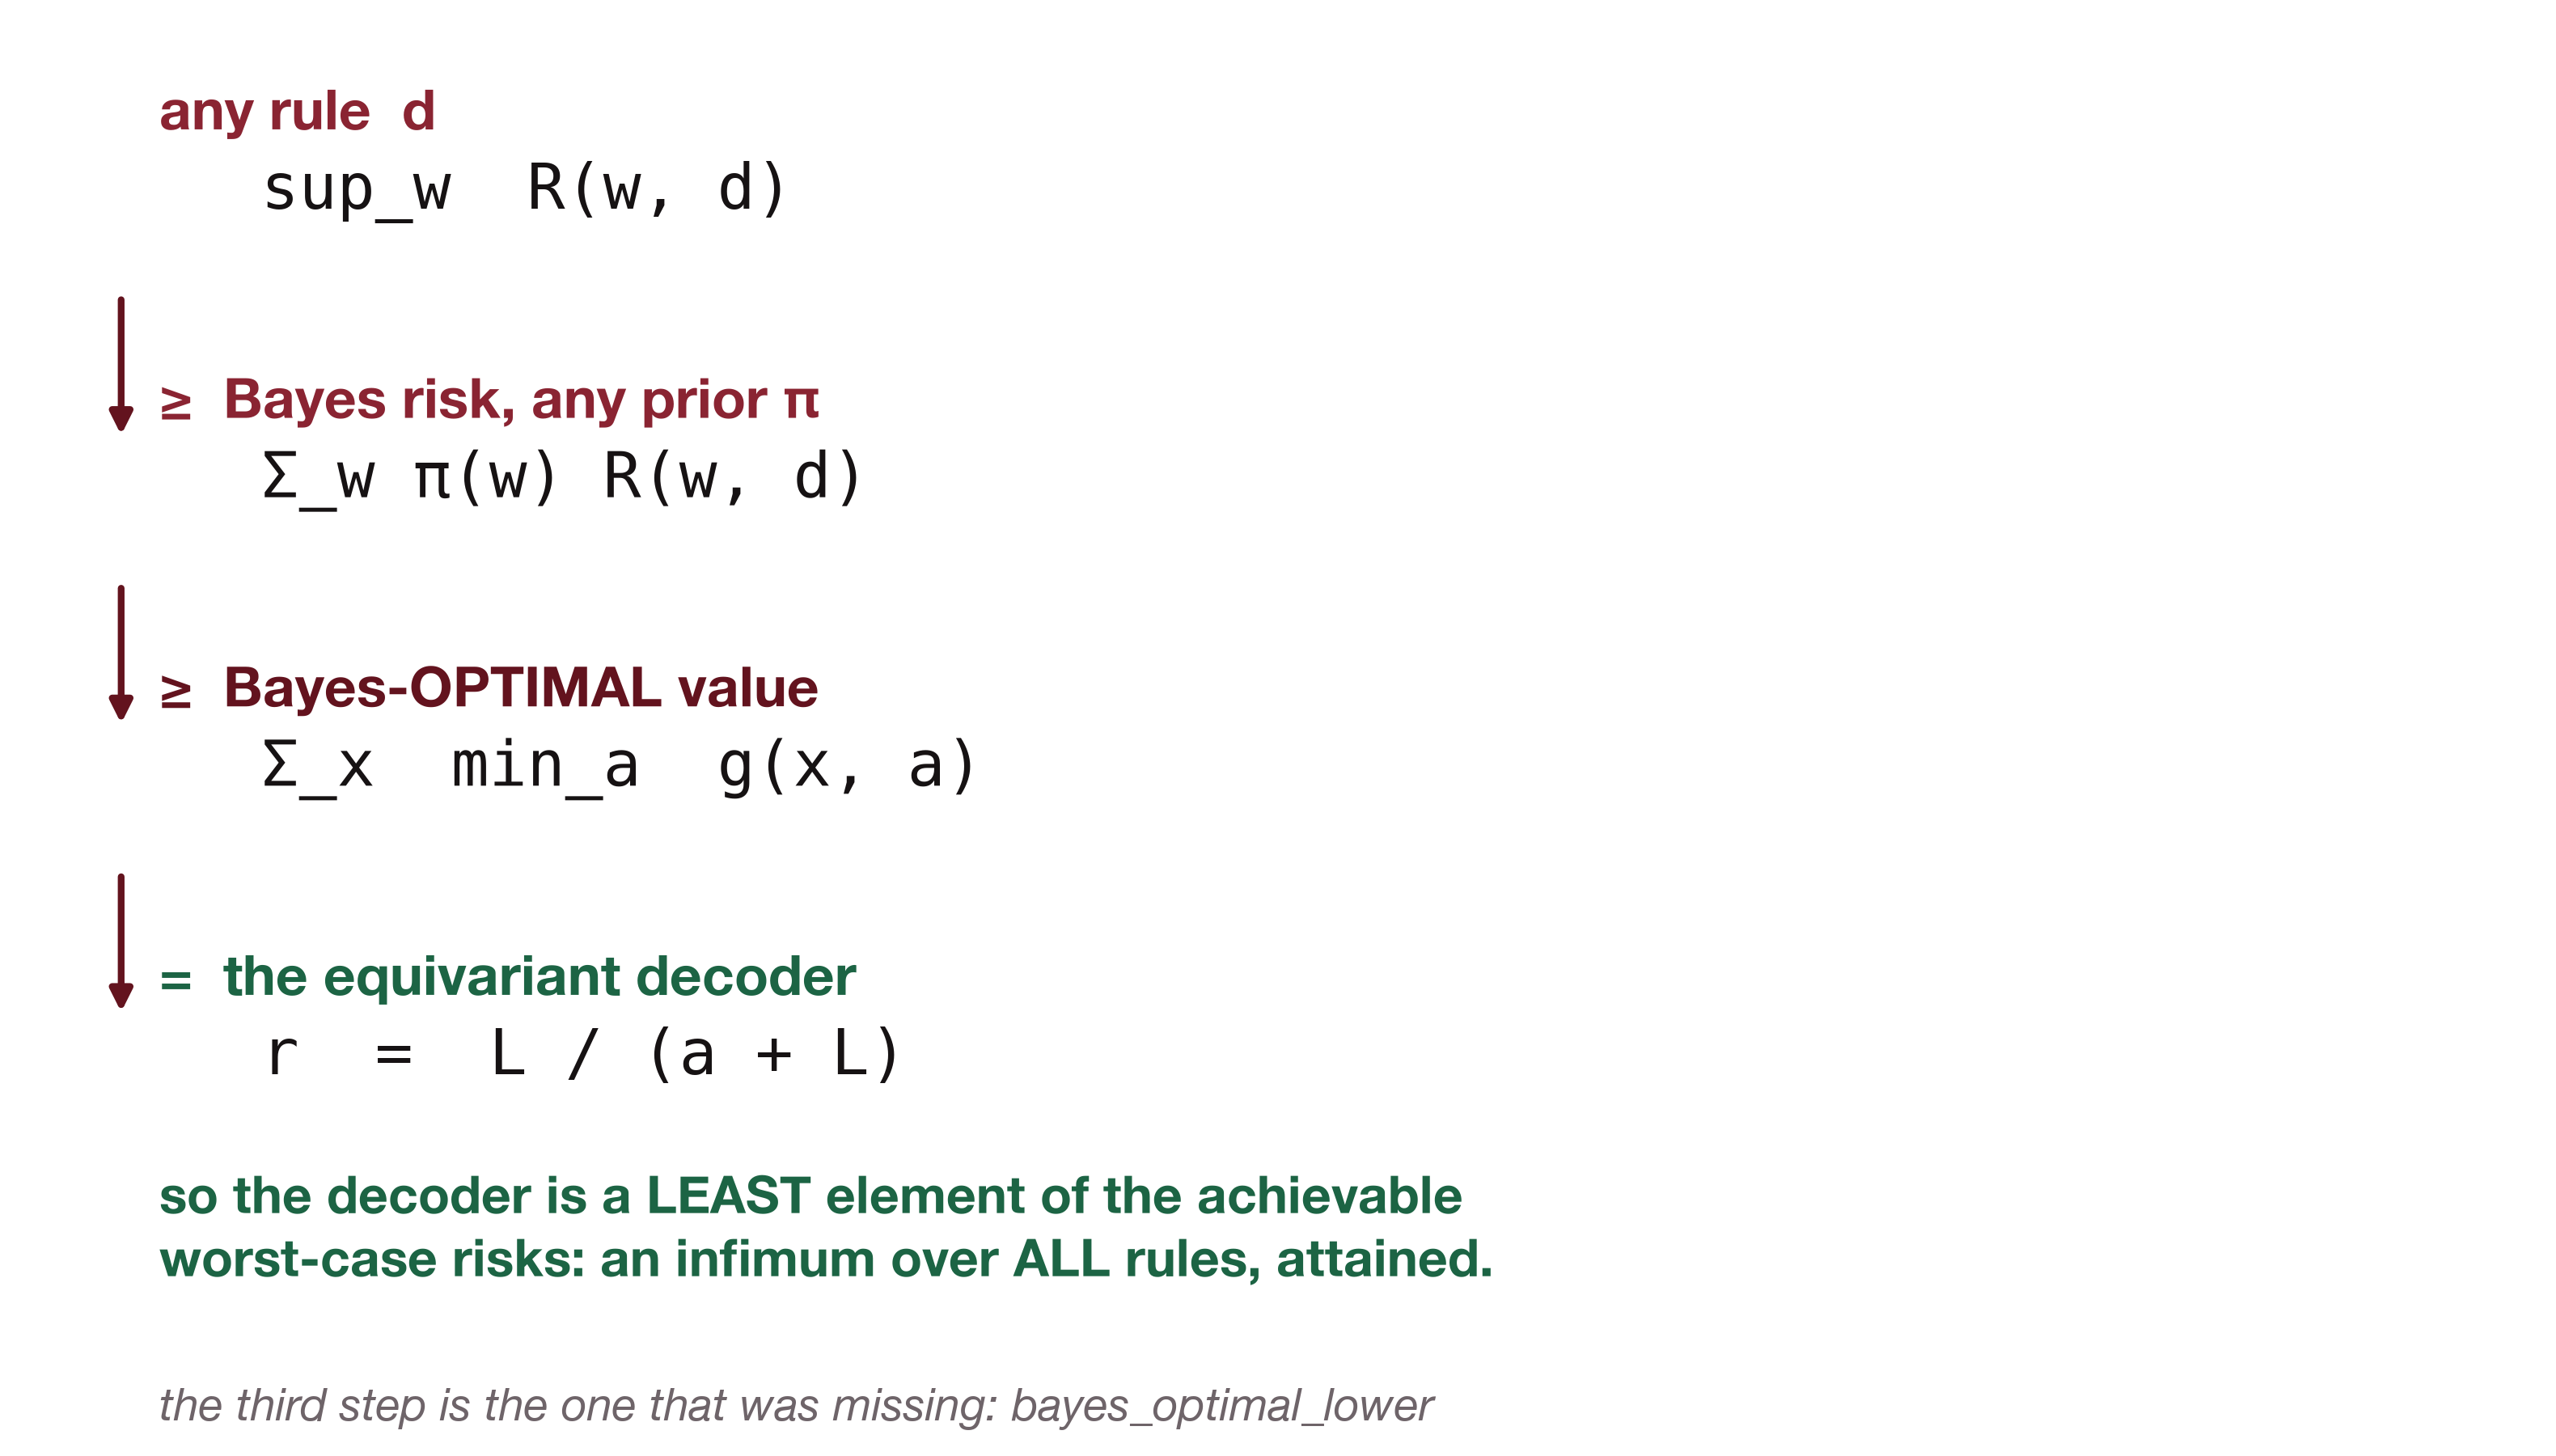
\includegraphics[width=\columnwidth]{support_fig2_minimax.png}
\caption{The minimax chain. Bayes risk factors through the posterior loss; the pointwise
minimum lower-bounds every rule and is attained; the worst case dominates the Bayes risk; and
the equivariant decoder's constant risk meets the resulting bound. The third step---optimality
over \emph{all} rules---is the one that was missing.}
\label{fig:sp-minimax}
\end{figure}

\subsection{Why the Decoder Is the Natural One}
\label{sec:sp-natural}

Theorem~\ref{thm:sp-minimax} says the equivariant decoder is optimal. It does not explain why
that decoder, of all rules, meets the bound, and the explanation is short.

Fix a relabelling-invariant prior. The posterior at a transcript $R$ is uniform over the
compatible worlds by symmetry, and by Lemma~\ref{lem:sp-hidden} each compatible world has exactly
$L$ unsafe tips among the $a+L$ unexplored ones. Summing over compatible worlds, each
unexplored tip is unsafe in the same number of them, so the posterior probability that a given
unexplored tip is unsafe is $L/(a+L)$, identically for every unexplored tip. The posterior
loss $g(x,a)$ is therefore constant across unexplored tips and strictly larger for explored
ones, which are known to be unsafe.

An immediate consequence is that the decoder is not \emph{uniquely} optimal: every rule naming
some unexplored tip is Bayes-optimal at that transcript. What all optimal rules share is the
constraint---never name an explored tip---and the freedom is in which unexplored one. This
identifies what the result actually rules out. It does not say randomisation helps or that the
uniform choice is special; it says the information in the transcript is exhausted by the set of
explored tips, so a rule weighting unexplored tips by some heuristic cannot do better, because
there is nothing left to be clever about.

The argument uses relabelling invariance twice, and with an asymmetric prior neither step
survives: the posterior loss varies across unexplored tips and the argmin is no longer the
uniform rule. Theorems~\ref{thm:sp-factor} and \ref{thm:sp-optimal} still hold, since they assume
nothing about the prior; what fails is the identification of the argmin with \emph{this}
decoder.

\begin{figure}[htbp]
\centering
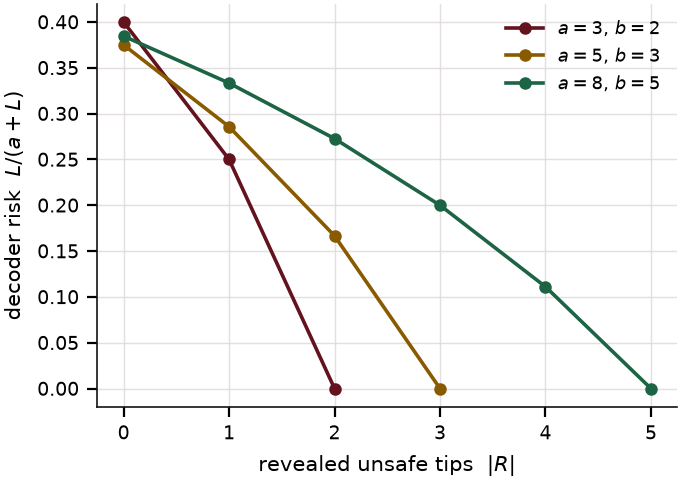
\includegraphics[width=\columnwidth]{support_fig3_risk.png}
\caption{What one revealed tip is worth. The decoder's risk is $L/(a+L)$ where $L$ is the
number of unsafe tips still unresolved, so revealing tips does not reduce risk linearly: each
one removes a term from the numerator and the denominator at once, and the curve is therefore
convex and steepest at the end. The three series are the safe/unsafe counts $(a,b)$ marked.
The practical reading is that the last few revelations carry most of the risk reduction,
which is the opposite of what a linear accounting of ``fraction revealed'' would suggest.
Exact evaluation of the decoder risk of Theorem~\ref{thm:sp-optimal}.}
\label{fig:sp-risk}
\end{figure}

\subsection{Pairwise Safety Does Not Suffice, in the Real Geometry}
\label{sec:sp-threeworld}

The minimax chain above concerns a single class. Across classes a second question arises, and
it is the one the decision-region literature identifies: a decision safe for every \emph{pair}
of surviving worlds need not be safe for all of them at once \cite{javdani2014}. That
phenomenon is easy to exhibit against an abstract regret function, which establishes only that
the abstract API permits it. We realise it inside the support-radius model the rest of the
development uses.

Take three relations and three worlds, each world having support $\{\text{anchor},\,
\mathrm{tip}(w)\}$ with anchor $(0,0,0)$, and let component $j$ read coordinate $j$. Set
\begin{align}
\mathrm{tip}(0)&=(\phantom{-}1,\phantom{-}1,-1), \notag\\
\mathrm{tip}(1)&=(-1,\phantom{-}1,\phantom{-}1), \notag\\
\mathrm{tip}(2)&=(\phantom{-}1,-1,\phantom{-}1).
\label{eq:sp-tips}
\end{align}

\begin{proposition}[Radius of a retained singleton]
\label{prop:sp-radius}
For every world $w$ and relation $j$,
\begin{equation}
\mathrm{selectedRadius}\bigl(F_{w},\{j\}\bigr)
\;=\;\frac{\bigl|\sum_{l\neq j}\mathrm{tip}(w)_{l}\bigr|}{2}.
\label{eq:sp-radius}
\end{equation}
\end{proposition}

\leanbox{\lean{radius\_formula}, \lean{zeroRegret\_spec} in
\lean{LeanSupportThreeWorldWitnessV1}}

Equation \eqref{eq:sp-radius} is what ties the construction to the corpus rather than to a toy:
the regret of keeping relation $j$ is half the oscillation of the sum of the omitted
relations, which is the quantity the rest of the development uses. Evaluating it on
\eqref{eq:sp-tips} gives radii $(0,0,1)$, $(1,0,0)$ and $(0,1,0)$ for the three worlds, so the
zero-regret decision sets are $\{0,1\}$, $\{1,2\}$ and $\{0,2\}$.

\begin{theorem}[Pairwise safety is not whole-fibre safety]
\label{thm:sp-threeworld}
On the construction \eqref{eq:sp-tips},
\begin{multline}
\bigl(\forall w,w'\;\exists j:\;
 \mathrm{selectedRadius}(F_{w},\{j\})=0 \\ \wedge\;
 \mathrm{selectedRadius}(F_{w'},\{j\})=0\bigr)
\;\wedge\;\\
\neg\,\exists j\;\forall w:\;\mathrm{selectedRadius}(F_{w},\{j\})=0 .
\label{eq:sp-threeworld}
\end{multline}
\end{theorem}

\begin{proof}
The three zero-regret sets pairwise intersect---$\{0,1\}\cap\{1,2\}=\{1\}$,
$\{1,2\}\cap\{0,2\}=\{2\}$, $\{0,1\}\cap\{0,2\}=\{0\}$---but their triple intersection is
empty.
\end{proof}

\leanbox{\lean{pairwise\_common\_decision}, \lean{no\_common\_decision},
\lean{pairwise\_not\_sufficient\_in\_support\_model} in
\lean{LeanSupportThreeWorldWitnessV1}}

Three points about this statement are worth making. It uses no \texttt{native\_decide} and no
decision procedure over the reals; the two \texttt{decide} calls are over a three-element
\lean{Finset (Fin 3)}. It is stated on \lean{selectedRadius} rather than on an abstract
regret, so it establishes the obstruction in the model rather than merely in the API. And it
bounds what a pairwise test can certify: a procedure verifying safety two worlds at a time
will pass this instance and be wrong, which is exactly the failure the Hyperedge Cutting
construction is designed to handle \cite{javdani2014}.

What the witness does \emph{not} give is a law. It exhibits a minimal unsafe triple; it does
not bound the size of the smallest such group as a function of the geometry, and
Section~\ref{sec:sp-discussion} lists that as the open problem it is.

\begin{figure}[htbp]
\centering
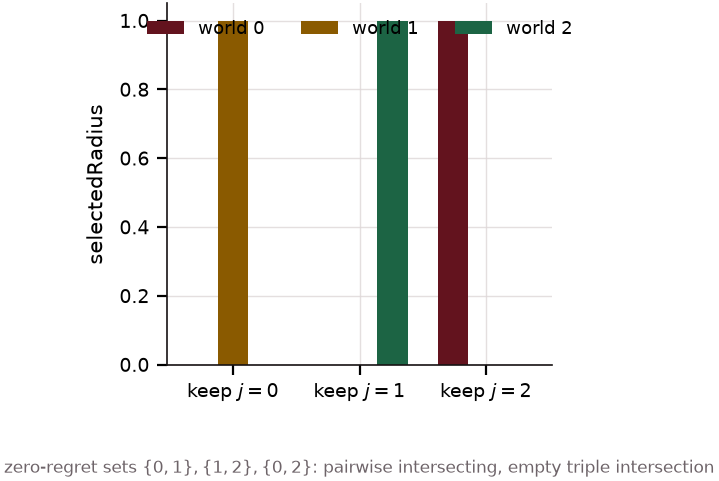
\includegraphics[width=\columnwidth]{support_fig5_threeworld.png}
\caption{The obstruction that pairwise reasoning cannot see, in the three-world model of
\lean{pairwise\_not\_sufficient\_in\_support\_model}. Each group of bars is one choice of the
coordinate kept; each bar within it is one world's selected radius. Every \emph{pair} of
worlds admits a kept coordinate at which both have zero radius---the three zero-regret sets
$\{0,1\}$, $\{1,2\}$ and $\{0,2\}$---so a procedure that checks safety two worlds at a time
finds nothing wrong. No coordinate works for all three at once: the three sets intersect
pairwise and their triple intersection is empty. The failure is a Helly-type one and is
invisible to any pairwise certificate, which is why the sufficiency argument has to be made
on the whole fibre.}
\label{fig:sp-threeworld}
\end{figure}

\subsection{The Decide--Recover Separation}
\label{sec:sp-separation}

Before the numbers, the two costs must be tied to an error criterion, since ``deciding'' and
``recovering'' are informal until they are.

\emph{Deciding} means: after $N$ observations, name one tip and be wrong with probability at
most $\varepsilon$, where wrong means the named tip is unsafe. \emph{Recovering} means: report
the full unsafe set across all classes and be wrong with probability at most $\varepsilon$.
Both costs are the least $N$ meeting the same $\varepsilon$, so the comparison is between two
thresholds computed the same way rather than between an exact quantity and an asymptotic rate.

\begin{theorem}[Exact separation]
\label{thm:sp-separation}
In the symmetric model the decide risk is
\begin{equation}
R_{\mathrm{dec}}\;=\;\frac{1}{2}(1-P)^{N}
\quad\text{exactly, flat in } K,
\label{eq:sp-decide}
\end{equation}
while the recovery cost grows with $K$.
\end{theorem}

\begin{proof}[Proof outline]
The decide risk collapses to \eqref{eq:sp-decide} by Theorem~\ref{thm:sp-sampling} and the
equivariant form \eqref{eq:sp-decoder}. The expression does not mention $K$ because a decision is
correct as soon as the named tip is safe, and that event's probability is settled inside a
single class; the other $K-1$ classes contribute nothing. The recovery cost is computed from
an inclusion--exclusion identity over the classes and is bounded below by a coupon-collector
argument.
\end{proof}

\leanbox{\lean{binary\_decide\_value}, \lean{decide\_upper\_expect},
\lean{growing\_K\_recover} in \lean{LeanSupportDecideRecoverV1}}

\noindent\emph{Supporting results in \lean{LeanSupportDecideRecoverV1}.}~These are the separation. The decide value is computed exactly and the monotonicity and factor bounds are what keep it independent of the number of classes; the recovery side is bounded pointwise and then in expectation, so the comparison is between an identity and a growth rate rather than between two estimates. They are reproduced as the prover has them; a further $5$ audited declarations in this module are positivity checks and measurability side conditions and are not displayed.

\noindent\textbf{S\,19}\quad\lean{binary\_decide\_value}
{\footnotesize\[ \begin{aligned}[t]
&[\mathit{Nonempty} \iota ],\; (\mathit{L} : \iota \to \mathbb{N} ),\; (\mathit{hL} : \forall \mathit{i}, \mathit{L} \mathit{i} \leq 1)\\
\vdash\;&(\mathit{univ}.\mathit{inf'} \mathit{univ\_nonempty} (\mathbf{fun} \mathit{i} => (\mathit{L} \mathit{i} : \mathbb{R} ) / (1 + \mathit{L} \mathit{i})))\\
&\quad = \mathbf{if} (\forall \mathit{i}, \mathit{L} \mathit{i} = 1) \mathbf{then} (1 : \mathbb{R} ) / 2 \mathbf{else} 0
\end{aligned} \]}

\noindent\textbf{S\,20}\quad\lean{cfac\_le\_one}
{\footnotesize\[ (\mathit{a} \mathit{L} : \iota \to \mathbb{N} ),\; (\mathit{i} : \iota ) \;\vdash\; \mathit{cfac} \mathit{a} \mathit{L} \mathit{i} \leq 1 \]}

\noindent\textbf{S\,21}\quad\lean{growing\_K\_recover}
{\footnotesize\[ \begin{aligned}[t]
&(\mathit{L} : \iota \to \mathbb{N} ),\; (\mathit{hL} : \forall \mathit{i}, \mathit{L} \mathit{i} \leq 1)\\
\vdash\;&\textstyle\prod \mathit{i}, (1 / ((((1:\mathbb{N} ) + \mathit{L} \mathit{i}).\mathit{choose} (\mathit{L} \mathit{i}) : \mathbb{N} ) : \mathbb{R} )) =\\
&\quad (1 / 2 : \mathbb{R} ) ^{} (\mathit{univ}.\mathit{filter} (\mathbf{fun} \mathit{i} => \mathit{L} \mathit{i} = 1)).\mathit{card}
\end{aligned} \]}

\noindent\textbf{S\,22}\quad\lean{recover\_lower\_pointwise}
{\footnotesize\[ \begin{aligned}[t]
&(\mathit{a} \mathit{L} : \iota \to \mathbb{N} ),\; (\mathit{ha} : \forall \mathit{i}, 1 \leq \mathit{a} \mathit{i}),\; (\mathit{i₀} : \iota ),\; (\mathit{h} : 1 \leq \mathit{L} \mathit{i₀})\\
\vdash\;&(1:\mathbb{R} ) / 2 \leq 1 - \textstyle\prod \mathit{i}, \mathit{cfac} \mathit{a} \mathit{L} \mathit{i}
\end{aligned} \]}

\noindent\textbf{S\,23}\quad\lean{recover\_upper\_pointwise}
{\footnotesize\[ (\mathit{a} \mathit{L} : \iota \to \mathbb{N} ) \;\vdash\; 1 - \textstyle\prod \mathit{i}, \mathit{cfac} \mathit{a} \mathit{L} \mathit{i} \leq \textstyle\sum \mathit{i}, (\mathit{L} \mathit{i} : \mathbb{R} ) \]}

\noindent\textbf{S\,24}\quad\lean{two\_le\_choose}
{\footnotesize\[ (\mathit{a} \mathit{L} : \mathbb{N} ),\; (\mathit{ha} : 1 \leq \mathit{a}),\; (\mathit{hL} : 1 \leq \mathit{L}) \;\vdash\; 2 \leq (\mathit{a} + \mathit{L}).\mathit{choose} \mathit{L} \]}


The recovery side is computed as an identity rather than a bound, and this matters because an
independence assumption would weaken the comparison. The probability that recovery is
incomplete is
\begin{equation}
R_{\mathrm{rec}}
\;=\;1-\sum_{k}\binom{K}{k}\Bigl(-\tfrac12\Bigr)^{k}
     \Bigl(1-\tfrac{kP}{K}\Bigr)^{N},
\label{eq:sp-recover}
\end{equation}
which assumes nothing about how the classes interact. The same quantity is sandwiched between
$\tfrac12\Pr(U>0)$ and $\Pr(U>0)$, verified exactly at several $N$, which is what allows the
coupon-collector scale to be quoted for orientation without being relied on.


\section{Part II: The Admissible Query Sets the Leakage Order}

\label{sec:qy-setting}

\subsection{Framework Overview}

An \emph{admissible measurement} is a choice of the perturbation map $g$ together with the
index set and weights; two measurements of the same pair of worlds share $f_{0},f_{1}$ and
differ in $g$. A \emph{level} is a value taken by the response, and the level structure is
what \eqref{eq:qy-assembly} sums over.

A distinction is maintained throughout. The leakage order $r$ is a property of the
\emph{expansion} of \eqref{eq:qy-mixture}, not of any estimator; the sample counts of
Section~\ref{sec:qy-samples} are what that order implies for an optimal test, and no claim is
made that a particular procedure attains them.

\subsection{Simplifying Assumptions}

\begin{enumerate}
\item[1)] \textbf{Dropped normalisation.} The constants $1/(\sigma\sqrt{2\pi})$ and $1/j!$ are
omitted from the algebraic displays, which is harmless for order statements because they are
invariant under positive scaling; the displayed expressions must not be quoted as densities.
The factorial is \emph{not} dropped where a constant is asserted. Since $\Delta_{r}$ is the
$r$-th derivative and not the Taylor coefficient, the leading difference between the two
densities is $h^{r}\Delta_{r}/r!$, and the $1/(r!)^{2}$ this produces is carried explicitly in
Theorem~\ref{thm:qy-sandwich} and Theorem~\ref{thm:qy-limit}. It cancels in their ratio, which is
why the width of the window in Section~\ref{sec:qy-sandwich} is unaffected.

\item[2)] \textbf{Shared level set.} The two worlds take values in the same finite level
set. This is what lets the order-$j$ coefficients pair term by term in
Theorem~\ref{thm:qy-cancel}; worlds with disjoint level structure are outside every statement
here.

\item[3)] \textbf{The top level carries weight.} At order $r$ the largest level of the shared
level set has a non-zero coefficient. This is the hypothesis
Theorem~\ref{thm:qy-nonvanish} needs. It is worth stating in this form rather than as a
strictness condition: levels are distinct reals, so the largest is automatically strictly
largest and nothing is assumed by saying so. What is assumed is that the coefficient there
does not vanish, and Section~\ref{sec:qy-nonvanish} says what is and is not known when it does.

\item[4)] \textbf{Fixed pair, fixed query.} Every result concerns one pair of worlds and one
admissible measurement. Nothing is a statement about the worst case over a class.
\end{enumerate}

\subsection{The Gaussian Derivatives, Built}
\label{sec:qy-hermite}

The expansion in $h$ is an iterated derivative, so the first task is an explicit form for the
iterated derivatives of a Gaussian. We build them rather than cite them, because the
non-vanishing argument needs one specific fact---the value of the leading coefficient---and
that fact must be available as a checked statement about this object.

\begin{theorem}[Hermite-type sequence]
\label{thm:qy-hermite}
There is a sequence of polynomials $H_{n}$ with
\begin{equation}
\frac{d^{\,n}}{dy^{\,n}}\,e^{-y^{2}/2\sigma^{2}}
   \;=\;H_{n}(y)\,e^{-y^{2}/2\sigma^{2}},
\label{eq:qy-hermite}
\end{equation}
and the degree-$n$ coefficient of $H_{n}$ equals $(-1/\sigma^{2})^{n}\neq0$. In particular
$H_{n}\neq0$ for every $n$.
\end{theorem}

\begin{proof}
Induction on $n$, with $H_{0}=1$. Differentiating the product gives
$H_{n+1}=H_{n}'-\tfrac{y}{\sigma^{2}}H_{n}$. The first term lowers degree and the second
raises it by one, multiplying the leading coefficient by $-1/\sigma^{2}$; the claim follows
by induction, and a polynomial with a non-zero coefficient is non-zero.
\end{proof}

\leanbox{\lean{iteratedDeriv\_gauss}, \lean{hpoly\_coeff}, \lean{hpoly\_ne\_zero} in
\lean{LeanQueryGaussianLevelV1}}

The statement about the leading coefficient is not decoration. It is exactly what
Section~\ref{sec:qy-nonvanish} consumes: without a non-zero top coefficient the contradiction
there does not close, and the leakage order would remain undefined.

\subsection{Pushing the Derivative Through the Sum}
\label{sec:qy-assembly}

Theorem~\ref{thm:qy-hermite} differentiates one mixture component. The observation law is a
finite sum of components, so the derivative must be moved inside the sum. Mathlib provides
the multilinear version of this exchange but not the scalar one, so we prove it.

\begin{theorem}[Scalar iterated-derivative sum rule]
\label{thm:qy-sumswap}
For a finite family $(F_{x})$ of functions each $C^{\infty}$ near $0$,
\begin{equation}
\left.\partial_{h}^{\,j}\right|_{h=0}\sum_{x}F_{x}(h)
   \;=\;\sum_{x}\left.\partial_{h}^{\,j}\right|_{h=0}F_{x}(h).
\label{eq:qy-sumswap}
\end{equation}
\end{theorem}

\begin{proof}
Mathlib's \lean{iteratedFDeriv\_fun\_sum\_apply} gives the Fréchet iterated derivative of a
finite sum. The scalar iterated derivative is that object evaluated at the all-ones vector,
so \eqref{eq:qy-sumswap} follows once the smoothness hypothesis is discharged for each summand.
Smoothness of a mixture component is proved from smoothness of $\exp$ composed with a
polynomial in $h$, not assumed.
\end{proof}

\leanbox{\lean{iteratedDeriv\_fun\_sum}, \lean{contDiff\_component},
\lean{iteratedDeriv\_mixture} in \lean{LeanQueryMixtureDerivativeV1}}

Combining Theorems~\ref{thm:qy-hermite} and \ref{thm:qy-sumswap} and grouping the components by
the level $v=f_{W}(x)$ they sit at gives the assembly
\begin{equation}
\Delta_{j}(y)\;=\;\sum_{v}M_{j}(v)\;H_{j}(y-v)\,\varphi_{\sigma}(y-v),
\label{eq:qy-assembly}
\end{equation}
where $M_{j}(v)$ collects the mixture weights at level $v$. Equation~\eqref{eq:qy-assembly} is
the form the whole paper turns on: each term is shifted to its own level, so no term-by-term
comparison is available, and whether the sum vanishes is a genuine question rather than a
computation.

\begin{figure}[htbp]
\centering
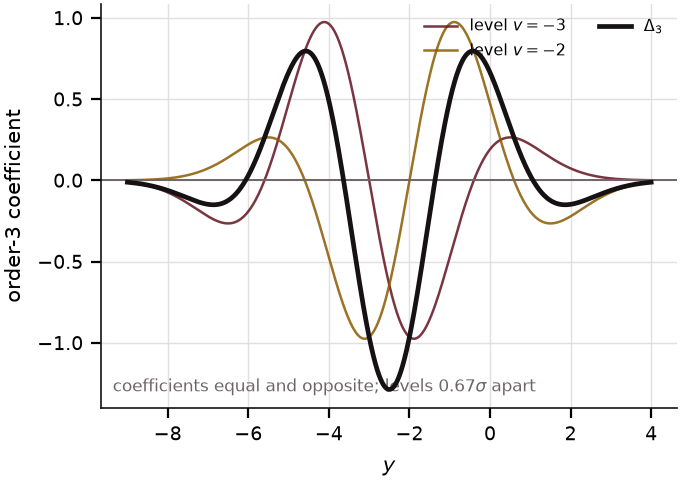
\includegraphics[width=\columnwidth]{query_fig8_assembly.png}
\caption{The assembly \eqref{eq:qy-assembly} at order three, evaluated exactly on a drawn
instance. Each thin curve is one level's term, a Hermite polynomial times a Gaussian shifted
to that level; the thick curve is their sum, which is $\Delta_{3}$. The two contributing
levels carry \emph{equal and opposite} coefficients---the exchange that defines the instance
moves the same weighted moment out of one level and into the other---so the two terms would
cancel identically if the levels coincided, and what survives is a consequence of their being
shifted apart. That is precisely why non-vanishing is the hard half of
Definition~\eqref{eq:qy-order}: no term-by-term comparison is available, and the sum's fate
depends on the geometry of the level set rather than on any individual coefficient. The
instance shown is the closest spacing the draw permits, $0.67\sigma$.}
\label{fig:qy-assembly}
\end{figure}

\subsection{Cancellation Below the Order}
\label{sec:qy-cancel}

Definition \eqref{eq:qy-order} has two halves. This subsection disposes of the easy one, both
for completeness and to make precise what ``the coefficients below order $r$ cancel'' means.

\begin{theorem}[Cancellation below the order]
\label{thm:qy-cancel}
Suppose the two worlds share a level set and that at order $j<r$ the level coefficients
satisfy $M^{(0)}_{j}(v)=M^{(1)}_{j}(v)$ for every level $v$. Then $\Delta_{j}\equiv0$.
\end{theorem}

\begin{proof}
By Theorem~\ref{thm:qy-sumswap} the order-$j$ coefficient of each world is the finite level sum
\eqref{eq:qy-assembly} with that world's coefficients. The shared level set makes the two sums
range over the same index set, so they pair term by term; corresponding coefficients agree,
so the difference is a sum of zero terms.
\end{proof}

\leanbox{\lean{mixture\_coeff\_diff\_eq\_zero} in \lean{LeanQueryMixtureDerivativeV1}}

The proof is short, and that is the point. Cancellation below the order is bookkeeping: the
terms agree, so their difference vanishes, and the hypotheses are checkable by inspecting
the mixture data. The converse situation---showing that a sum of terms which do \emph{not}
pair off is nonetheless non-zero as a function---has no such structure, which is why the next
subsection is the length it is.

\subsection{Non-Vanishing: the Hard Half}
\label{sec:qy-nonvanish}

Fix the order $r$ and let $v^{*}$ be the largest level carrying a non-zero coefficient.
Factoring the Gaussian at level $v^{*}$ out of $\Delta_{r}$ leaves
\begin{equation}
T(y)\;=\;c_{v^{*}}H_{r}(y-v^{*})\;+\;\sum_{v<v^{*}}c_{v}\,H_{r}(y-v).
\label{eq:qy-nonvanish}
\end{equation}
The expression is written this way because the factorisation is what separates the terms: it
converts a sum of equal-footing shifted Gaussians into one polynomial plus a remainder that
decays.

\begin{theorem}[The order-$r$ coefficient does not vanish]
\label{thm:qy-nonvanish}
If $c_{v^{*}}\neq0$ and $v^{*}$ is strictly the largest level, then $T\not\equiv0$;
consequently $\Delta_{r}\not\equiv0$ and the leakage order \eqref{eq:qy-order} is well defined.
\end{theorem}

\begin{proof}
After the factorisation, each term with $v<v^{*}$ carries the ratio
$\varphi_{\sigma}(y-v)/\varphi_{\sigma}(y-v^{*})
=\exp\bigl(-(v^{*}-v)(y-\tfrac{v+v^{*}}{2})/\sigma^{2}\bigr)$, which decays to $0$ as
$y\to+\infty$ because $v^{*}-v>0$. Each such term is therefore a polynomial against a
decaying exponential and tends to $0$.

Suppose $T\equiv0$. Then along $y\to+\infty$ the surviving term $c_{v^{*}}H_{r}(y-v^{*})$
must tend to $0$ as well. A polynomial tending to $0$ at $+\infty$ has vanishing leading
coefficient, so $c_{v^{*}}$ times the degree-$r$ coefficient of $H_{r}$ is zero. But
$c_{v^{*}}\neq0$ by hypothesis and that coefficient is $(-1/\sigma^{2})^{r}\neq0$ by
Theorem~\ref{thm:qy-hermite}---a contradiction.
\end{proof}

\leanbox{\lean{levelSum\_ne\_zero} in \lean{LeanQueryGaussianLevelV1};
\lean{mixture\_coeff\_ne\_zero} in \lean{LeanQueryMixtureDerivativeV1}}

\noindent\emph{Supporting results in \lean{LeanQueryGaussianLevelV1}.}~These build the Gaussian derivatives and prove the one fact the crux argument consumes. The first group establishes the product form \eqref{eq:qy-hermite} and the positivity and shift properties the factorisation in \eqref{eq:qy-nonvanish} needs. The degree bound and the leading coefficient are separate statements because the contradiction in Theorem~\ref{thm:qy-nonvanish} uses the coefficient specifically: a polynomial tending to zero at $+\infty$ must have it vanish, and here it cannot. They are reproduced as the prover has them; a further $2$ audited declarations in this module are positivity checks and measurability side conditions and are not displayed.
\TODOPAR{Formalisation gap worth closing, and it is small. \lean{levelSum\_ne\_zero}
takes $S:\mathsf{Finset}\ \mathbb{R}$ with $v^{*}$ strictly greatest and $c_{v^{*}}\neq0$.
Since a finite set of reals always has a unique maximum, the strictness hypothesis restricts
nothing; the only real hypothesis is $c_{v^{*}}\neq0$. The uncovered case is therefore a
vanishing top coefficient, and it is closed by restricting the sum to
$S.\mathrm{filter}\,(c\neq0)$ and applying the same theorem at the largest surviving level---a
few lines with \lean{Finset.max'} and \lean{Finset.filter\_nonempty\_iff}. Doing it would
strengthen Theorem~\ref{thm:qy-nonvanish} to ``$\Delta_{r}\not\equiv0$ iff the level-coefficient
vector is not identically zero'', remove the \textsc{undetermined} branch from
Algorithm~\ref{alg:qy-order}, and delete an open problem that does not exist.}

\noindent\textbf{S\,1}\quad\lean{gauss\_shift}
{\footnotesize\[ \begin{aligned}[t]
&(\sigma : \mathbb{R} ),\; (\mathit{hσ} : \sigma \neq 0),\; (\mathit{v} \mathit{y} : \mathbb{R} )\\
\vdash\;&\mathit{gauss} \sigma (\mathit{y} - \mathit{v}) = \mathit{gauss} \sigma \mathit{y} * \mathit{Real}.\mathit{exp} (\mathit{v} * \mathit{y} / \sigma ^{2} - \mathit{v} ^{2} / (2 * \sigma ^{2}))
\end{aligned} \]}

\noindent\textbf{S\,2}\quad\lean{hasDerivAt\_gauss}
{\footnotesize\[ \begin{aligned}[t]
&(\sigma : \mathbb{R} ),\; (\mathit{hσ} : \sigma \neq 0),\; (\mathit{y} : \mathbb{R} )\\
\vdash\;&\mathit{HasDerivAt} (\mathit{gauss} \sigma ) (-(\mathit{y} / \sigma ^{2}) * \mathit{gauss} \sigma \mathit{y}) \mathit{y}
\end{aligned} \]}

\noindent\textbf{S\,3}\quad\lean{hasDerivAt\_hgauss}
{\footnotesize\[ \begin{aligned}[t]
&(\sigma : \mathbb{R} ),\; (\mathit{hσ} : \sigma \neq 0),\; (\mathit{j} : \mathbb{N} ),\; (\mathit{z} : \mathbb{R} )\\
\vdash\;&\mathit{HasDerivAt} (\mathbf{fun} \mathit{w} => (\mathit{hpoly} \sigma \mathit{j}).\mathit{eval} \mathit{w} * \mathit{gauss} \sigma \mathit{w}) ((\mathit{hpoly} \sigma (\mathit{j}\\
&\quad + 1)).\mathit{eval} \mathit{z} * \mathit{gauss} \sigma \mathit{z}) \mathit{z}
\end{aligned} \]}

\noindent\textbf{S\,4}\quad\lean{hpoly\_coeff}
{\footnotesize\[ (\sigma : \mathbb{R} ) \;\vdash\; \forall \mathit{n} : \mathbb{N} , (\mathit{hpoly} \sigma \mathit{n}).\mathit{coeff} \mathit{n} = (-(1 / \sigma ^{2})) ^{\mathit{n}} \]}

\noindent\textbf{S\,5}\quad\lean{hpoly\_natDegree\_le}
{\footnotesize\[ (\sigma : \mathbb{R} ) \;\vdash\; \forall \mathit{n} : \mathbb{N} , (\mathit{hpoly} \sigma \mathit{n}).\mathit{natDegree} \leq \mathit{n} \]}

\noindent\textbf{S\,6}\quad\lean{hpoly\_ne\_zero}
{\footnotesize\[ (\sigma : \mathbb{R} ),\; (\mathit{hσ} : \sigma \neq 0),\; (\mathit{n} : \mathbb{N} ) \;\vdash\; \mathit{hpoly} \sigma \mathit{n} \neq 0 \]}

\noindent\textbf{S\,7}\quad\lean{iteratedDeriv\_gauss}
{\footnotesize\[ \begin{aligned}[t]
&(\sigma : \mathbb{R} ),\; (\mathit{hσ} : \sigma \neq 0)\\
\vdash\;&\forall (\mathit{n} : \mathbb{N} ) (\mathit{y} : \mathbb{R} ), \mathit{iteratedDeriv} \mathit{n} (\mathit{gauss} \sigma ) \mathit{y} = (\mathit{hpoly} \sigma \mathit{n}).\mathit{eval} \mathit{y}\\
&\quad * \mathit{gauss} \sigma \mathit{y}
\end{aligned} \]}

\noindent\textbf{S\,8}\quad\lean{iteratedDeriv\_shift}
{\footnotesize\[ \begin{aligned}[t]
&(\sigma : \mathbb{R} ),\; (\mathit{hσ} : \sigma \neq 0),\; (\mathit{g} \mathit{v} \mathit{y} : \mathbb{R} )\\
\vdash\;&\forall (\mathit{j} : \mathbb{N} ) (\mathit{h₀} : \mathbb{R} ), \mathit{iteratedDeriv} \mathit{j} (\mathbf{fun} \mathit{h} : \mathbb{R} => \mathit{gauss} \sigma (\mathit{y} - \mathit{v}\\
&\quad - \mathit{h} * \mathit{g})) \mathit{h₀} = (-\mathit{g}) ^{\mathit{j}} * ((\mathit{hpoly} \sigma \mathit{j}).\mathit{eval} (\mathit{y} - \mathit{v} - \mathit{h₀} * \mathit{g}) *\\
&\quad \mathit{gauss} \sigma (\mathit{y} - \mathit{v} - \mathit{h₀} * \mathit{g}))
\end{aligned} \]}

\noindent\textbf{S\,9}\quad\lean{levelSum\_eq\_zero\_of\_levels\_agree}
{\footnotesize\[ \begin{aligned}[t]
&(\sigma : \mathbb{R} ),\; (\mathit{r} : \mathbb{N} ),\; (\mathit{S} : \mathit{Finset} \mathbb{R} ),\; (\mathit{cA} \mathit{cB} : \mathbb{R} \to \mathbb{R} ),\\
&\quad \; (\mathit{hagree} : \forall \mathit{v} \in \mathit{S}, \mathit{cA} \mathit{v} = \mathit{cB} \mathit{v}),\; (\mathit{y} : \mathbb{R} )\\
\vdash\;&\mathit{levelSum} \sigma \mathit{r} \mathit{S} \mathit{cA} \mathit{y} - \mathit{levelSum} \sigma \mathit{r} \mathit{S} \mathit{cB} \mathit{y} = 0
\end{aligned} \]}

\noindent\textbf{S\,10}\quad\lean{levelSum\_ne\_zero}
{\footnotesize\[ \begin{aligned}[t]
&(\sigma : \mathbb{R} ),\; (\mathit{hσ} : \sigma \neq 0),\; (\mathit{r} : \mathbb{N} ),\; (\mathit{S} : \mathit{Finset} \mathbb{R} ),\\
&\quad \; (\mathit{c} : \mathbb{R} \to \mathbb{R} ),\; (\mathit{vstar} : \mathbb{R} ),\; (\mathit{hvs} : \mathit{vstar} \in \mathit{S}),\\
&\quad \; (\mathit{htop} : \forall \mathit{v} \in \mathit{S}, \mathit{v} \neq \mathit{vstar} \to \mathit{v} < \mathit{vstar}),\; (\mathit{hc} : \mathit{c} \mathit{vstar} \neq 0)\\
\vdash\;&\exists \mathit{y}, \mathit{levelSum} \sigma \mathit{r} \mathit{S} \mathit{c} \mathit{y} \neq 0
\end{aligned} \]}

\noindent\textbf{S\,11}\quad\lean{sum\_by\_level}
{\footnotesize\[ \begin{aligned}[t]
&\{ \mathit{X} : \mathit{Type}*\},\; [\mathit{Fintype} \mathit{X}],\; [\mathit{DecidableEq} \mathit{X}],\; (\mathit{pi} \mathit{f} \mathit{w} : \mathit{X} \to \mathbb{R} ),\\
&\quad \; (\mathit{Q} : \mathbb{R} \to \mathbb{R} )\\
\vdash\;&\textstyle\sum \mathit{x} : \mathit{X}, \mathit{pi} \mathit{x} * \mathit{w} \mathit{x} * \mathit{Q} (\mathit{f} \mathit{x}) = \textstyle\sum \mathit{v} \in \mathit{Finset}.\mathit{image} \mathit{f} \mathit{Finset}.\mathit{univ},\\
&\quad (\textstyle\sum \mathit{x} \in \mathit{Finset}.\mathit{univ}.\mathit{filter} (\mathbf{fun} \mathit{x} => \mathit{f} \mathit{x} = \mathit{v}), \mathit{pi} \mathit{x} * \mathit{w} \mathit{x}) *\\
&\quad \mathit{Q} \mathit{v}
\end{aligned} \]}


\noindent\emph{Supporting results in \lean{LeanQueryMixtureDerivativeV1}.}~These move the derivative through the finite mixture and state both halves of \eqref{eq:qy-order}. The smoothness of a component is proved rather than assumed, because mathlib's multilinear sum rule requires it and assuming it would leave the paper's own contribution resting on an unproved side condition. They are reproduced as the prover has them; a further $0$ audited declarations in this module are positivity checks and measurability side conditions and are not displayed.

\noindent\textbf{S\,12}\quad\lean{contDiff\_component}
{\footnotesize\[ \begin{aligned}[t]
&(\sigma : \mathbb{R} ),\; (\mathit{v} \mathit{g} \mathit{y} : \mathbb{R} ),\; (\mathit{n} : \mathbb{N} )\\
\vdash\;&\mathit{ContDiff} \mathbb{R} \mathit{n} (\mathbf{fun} \mathit{h} : \mathbb{R} => \mathit{gauss} \sigma (\mathit{y} - \mathit{v} - \mathit{h} * \mathit{g}))
\end{aligned} \]}

\noindent\textbf{S\,13}\quad\lean{iteratedDeriv\_fun\_sum}
{\footnotesize\[ \begin{aligned}[t]
&\{ \iota : \mathit{Type}*\},\; \{ \mathit{u} : \mathit{Finset} \iota \},\; \{ \mathit{n} : \mathbb{N} \},\; \{ \mathit{F} : \iota \to \mathbb{R} \to\\
&\quad \mathbb{R} \},\; \{ \mathit{x} : \mathbb{R} \},\; (\mathit{h} : \forall \mathit{i} \in \mathit{u}, \mathit{ContDiffAt} \mathbb{R} \mathit{n} (\mathit{F} \mathit{i}) \mathit{x})\\
\vdash\;&\mathit{iteratedDeriv} \mathit{n} (\mathbf{fun} \mathit{z} => \textstyle\sum \mathit{i} \in \mathit{u}, \mathit{F} \mathit{i} \mathit{z}) \mathit{x} = \textstyle\sum \mathit{i} \in \mathit{u},\\
&\quad \mathit{iteratedDeriv} \mathit{n} (\mathit{F} \mathit{i}) \mathit{x}
\end{aligned} \]}

\noindent\textbf{S\,14}\quad\lean{iteratedDeriv\_mixture}
{\footnotesize\[ \begin{aligned}[t]
&(\sigma : \mathbb{R} ),\; (\mathit{hσ} : \sigma \neq 0),\; (\mathit{pi} \mathit{f} \mathit{g} : \mathit{X} \to \mathbb{R} ),\; (\mathit{y} : \mathbb{R} ),\; (\mathit{j} : \mathbb{N} )\\
\vdash\;&\mathit{iteratedDeriv} \mathit{j} (\mathbf{fun} \mathit{h} : \mathbb{R} => \textstyle\sum \mathit{x} : \mathit{X}, \mathit{pi} \mathit{x} * \mathit{gauss} \sigma (\mathit{y} - \mathit{f} \mathit{x} - \mathit{h}\\
&\quad * \mathit{g} \mathit{x})) 0 = \mathit{levelSum} \sigma \mathit{j} (\mathit{Finset}.\mathit{image} \mathit{f} \mathit{Finset}.\mathit{univ}) (\\
&\quad \mathit{levelMoment} \mathit{pi} \mathit{f} \mathit{g} \mathit{j}) \mathit{y}
\end{aligned} \]}

\noindent\textbf{S\,15}\quad\lean{mixture\_coeff\_diff\_eq\_zero}
{\footnotesize\[ \begin{aligned}[t]
&(\sigma : \mathbb{R} ),\; (\mathit{hσ} : \sigma \neq 0),\; (\mathit{piA} \mathit{fA} \mathit{gA} \mathit{piB} \mathit{fB} \mathit{gB} : \mathit{X} \to \mathbb{R} ),\; (\mathit{j} : \mathbb{N} ),\\
&\quad \; (\mathit{y} : \mathbb{R} ),\; (\mathit{hS} : \mathit{Finset}.\mathit{image} \mathit{fB} \mathit{Finset}.\mathit{univ} = \mathit{Finset}.\mathit{image}\\
&\quad \mathit{fA} \mathit{Finset}.\mathit{univ}),\; (\mathit{hagree} : \forall \mathit{v} \in \mathit{Finset}.\mathit{image} \mathit{fA} \mathit{Finset}.\mathit{univ}\\
&\quad , \mathit{levelMoment} \mathit{piA} \mathit{fA} \mathit{gA} \mathit{j} \mathit{v} = \mathit{levelMoment} \mathit{piB} \mathit{fB} \mathit{gB} \mathit{j} \mathit{v})\\
\vdash\;&\mathit{iteratedDeriv} \mathit{j} (\mathbf{fun} \mathit{h} : \mathbb{R} => \textstyle\sum \mathit{x} : \mathit{X}, \mathit{piA} \mathit{x} * \mathit{gauss} \sigma (\mathit{y} - \mathit{fA} \mathit{x}\\
&\quad - \mathit{h} * \mathit{gA} \mathit{x})) 0 - \mathit{iteratedDeriv} \mathit{j} (\mathbf{fun} \mathit{h} : \mathbb{R} => \textstyle\sum \mathit{x} : \mathit{X},\\
&\quad \mathit{piB} \mathit{x} * \mathit{gauss} \sigma (\mathit{y} - \mathit{fB} \mathit{x} - \mathit{h} * \mathit{gB} \mathit{x})) 0 = 0
\end{aligned} \]}

\noindent\textbf{S\,16}\quad\lean{mixture\_coeff\_ne\_zero}
{\footnotesize\[ \begin{aligned}[t]
&(\sigma : \mathbb{R} ),\; (\mathit{hσ} : \sigma \neq 0),\; (\mathit{pi} \mathit{f} \mathit{g} : \mathit{X} \to \mathbb{R} ),\; (\mathit{r} : \mathbb{N} ),\\
&\quad \; (\mathit{vstar} : \mathbb{R} ),\; (\mathit{hvs} : \mathit{vstar} \in \mathit{Finset}.\mathit{image} \mathit{f} \mathit{Finset}.\mathit{univ}),\\
&\quad \; (\mathit{htop} : \forall \mathit{v} \in \mathit{Finset}.\mathit{image} \mathit{f} \mathit{Finset}.\mathit{univ}, \mathit{v} \neq \mathit{vstar} \to \mathit{v} <\\
&\quad \mathit{vstar}),\; (\mathit{hc} : \mathit{levelMoment} \mathit{pi} \mathit{f} \mathit{g} \mathit{r} \mathit{vstar} \neq 0)\\
\vdash\;&\exists \mathit{y}, \mathit{iteratedDeriv} \mathit{r} (\mathbf{fun} \mathit{h} : \mathbb{R} => \textstyle\sum \mathit{x} : \mathit{X}, \mathit{pi} \mathit{x} * \mathit{gauss} \sigma (\mathit{y} - \mathit{f} \mathit{x}\\
&\quad - \mathit{h} * \mathit{g} \mathit{x})) 0 \neq 0
\end{aligned} \]}


A word on what this hypothesis excludes, because it is easy to state it as more than it is.
The level set is a finite set of distinct reals, so it has a unique maximum and that maximum
is strictly greater than every other level; two \emph{distinct} levels cannot tie, and two
levels that coincide are one level whose coefficient is the sum of theirs. The hypothesis
therefore places no restriction on the level set at all. The single thing it asks is that
$c_{v^{*}}\neq0$ at the top level $v^{*}$.

The configuration it does exclude is the one where that coefficient vanishes while some lower
level still carries weight. That case is not hard---restricting the sum to the support of $c$
changes nothing, since a zero coefficient contributes nothing, and the theorem then applies
at the largest surviving level---but it is arithmetic done in prose here and not in Lean, so
Algorithm~\ref{alg:qy-order} reports \textsc{undetermined} rather than deciding it. The gap is
in the formalisation, not in the mathematics.

\subsection{The Hellinger Sandwich}
\label{sec:qy-sandwich}

\begin{theorem}[Two-sided sandwich with explicit constants]
\label{thm:qy-sandwich}
With $r$ the leakage order and constants $a_{E},J>0$ determined by the mixture,
\begin{equation}
\frac{a_{E}^{2}\,h^{2r}}{32\,(r!)^{2}}\;\leq\;H^{2}\;\leq\;\frac{J}{2\,(r!)^{2}}\,h^{2r}.
\label{eq:qy-sandwich}
\end{equation}
\end{theorem}

\begin{proof}[Proof outline]
\emph{Lower side.} Theorem~\ref{thm:qy-nonvanish} gives $\Delta_{r}\not\equiv0$, so by
continuity there is a bounded interval $E$ and $a_{E}>0$ with $|\Delta_{r}|\ge a_{E}$ on
$E$. On $E$ the two densities differ by $h^{r}\Delta_{r}/r!$ plus a uniform $O(h^{r+1})$
remainder---the factorial is the Taylor coefficient, and $\Delta_{r}$ is the derivative---so
for small $h$ the difference is at least $a_{E}h^{r}/(2\,r!)$ throughout $E$. The
Hellinger distance is bounded below through
$(\sqrt{p}-\sqrt{q})^{2}=(p-q)^{2}/(\sqrt{p}+\sqrt{q})^{2}$; bounding
$(\sqrt{p}+\sqrt{q})^{2}\le2(p+q)$ and applying Cauchy--Schwarz on $E$ gives, for every
$t>0$, a bound whose optimisation over $t$ yields the stated quadratic form. Tracking the
factors---two from the denominator bound, two from the remainder, two from the Hellinger
normalisation, four from the square---produces $32$.

\emph{Upper side.} Pointwise $(\sqrt{p}-\sqrt{q})^{2}\le(p-q)^{2}/q$, so the Hellinger
integrand is dominated by the $\chi^{2}$ integrand. Expanding $p-q$ to order $r$ with a
uniform Taylor remainder, and bounding the remainder by an integrable envelope that is
constructed and proved integrable rather than assumed, gives $H^{2}\le(J/2)h^{2r}$.
\end{proof}

\leanbox{\lean{hellinger\_lower\_from\_interval} in \lean{LeanQueryHellingerIntervalV1};
\lean{hellinger\_upper\_const} in \lean{LeanQueryTaylorRemainderV1}}

\noindent\emph{Supporting results in \lean{LeanQueryTaylorRemainderV1}.}~These supply the upper side of the sandwich. The envelope is constructed and its integrability proved; the $\chi^{2}$ comparison and the vanishing-derivative bound then convert a Taylor remainder into the constant $J/2$. The derivative-on-an-interval lemma appears because the remainder is controlled on a closed interval and the ambient derivative must be identified with the one-sided derivative there. They are reproduced as the prover has them; a further $2$ audited declarations in this module are positivity checks and measurability side conditions and are not displayed.

\noindent\textbf{S\,17}\quad\lean{bound\_of\_vanishing\_derivs}
{\footnotesize\[ \begin{aligned}[t]
&(\mathit{F} : \mathbb{R} \to \mathbb{R} ),\; (\mathit{n} : \mathbb{N} ),\; (\mathit{b} \mathit{C} : \mathbb{R} ),\; (\mathit{hb} : 0 < \mathit{b}),\\
&\quad \; (\mathit{hcd} : \mathit{ContDiffOn} \mathbb{R} (\mathit{n} + 1 : \mathbb{N} ) \mathit{F} (\mathit{Icc} 0 \mathit{b})),\; (\mathit{hv} : \forall \mathit{j} \leq \mathit{n},\\
&\quad \mathit{iteratedDerivWithin} \mathit{j} \mathit{F} (\mathit{Icc} 0 \mathit{b}) 0 = 0),\; (\mathit{hC} : \forall \mathit{y} \in \mathit{Icc} (0:\mathbb{R} ) \mathit{b},\\
&\quad |\mathit{iteratedDerivWithin} (\mathit{n} + 1) \mathit{F} (\mathit{Icc} 0 \mathit{b}) \mathit{y}| \leq \mathit{C})\\
\vdash\;&|\mathit{F} \mathit{b}| \leq \mathit{C} * \mathit{b} ^{} (\mathit{n} + 1) / \mathit{n} !
\end{aligned} \]}

\noindent\textbf{S\,18}\quad\lean{component\_deriv\_envelope}
{\footnotesize\[ \begin{aligned}[t]
&(\sigma \mathit{M} \mathit{g} \mathit{v} \mathit{y} \xi : \mathbb{R} ),\; (\mathit{r} : \mathbb{N} ),\; (\mathit{hσ} : 0 < \sigma ),\; (\mathit{hmv} : |\mathit{v} + \xi * \mathit{g}| \leq \mathit{M})\\
\vdash\;&|\mathit{iteratedDeriv} \mathit{r} (\mathbf{fun} \mathit{h} : \mathbb{R} => \mathit{gauss} \sigma (\mathit{y} - \mathit{v} - \mathit{h} * \mathit{g})) \xi | \leq\\
&\quad |\mathit{g}| ^{\mathit{r}} * |(\mathit{hpoly} \sigma \mathit{r}).\mathit{eval} (\mathit{y} - \mathit{v} - \xi * \mathit{g})| * \mathit{Real}.\mathit{exp} (-(\mathit{y} ^{2}) /\\
&\quad (2 * \sigma ^{2}) + \mathit{M} * |\mathit{y}| / \sigma ^{2})
\end{aligned} \]}

\noindent\textbf{S\,19}\quad\lean{derivWithin\_eq\_deriv\_on\_Icc}
{\footnotesize\[ \begin{aligned}[t]
&(\mathit{F} : \mathbb{R} \to \mathbb{R} ),\; (\mathit{n} : \mathbb{N} ),\; (\mathit{a} \mathit{b} \mathit{x} : \mathbb{R} ),\; (\mathit{hab} : \mathit{a} < \mathit{b}),\\
&\quad \; (\mathit{hF} : \mathit{ContDiff} \mathbb{R} (\mathit{n} : \mathbb{N} \infty ) \mathit{F}),\; (\mathit{hx} : \mathit{x} \in \mathit{Icc} \mathit{a} \mathit{b})\\
\vdash\;&\mathit{iteratedDerivWithin} \mathit{n} \mathit{F} (\mathit{Icc} \mathit{a} \mathit{b}) \mathit{x} = \mathit{iteratedDeriv} \mathit{n} \mathit{F} \mathit{x}
\end{aligned} \]}

\noindent\textbf{S\,20}\quad\lean{gaussComp\_contDiff}
{\footnotesize\[ \begin{aligned}[t]
&(\sigma \mathit{g} \mathit{v} \mathit{y} : \mathbb{R} )\\
\vdash\;&\mathit{ContDiff} \mathbb{R} (⊤ : \mathbb{N} \infty ) (\mathbf{fun} \mathit{h} : \mathbb{R} => \mathit{gauss} \sigma (\mathit{y} - \mathit{v} - \mathit{h} * \mathit{g}))
\end{aligned} \]}

\noindent\textbf{S\,21}\quad\lean{taylor\_vanishing\_zero}
{\footnotesize\[ \begin{aligned}[t]
&(\mathit{F} : \mathbb{R} \to \mathbb{R} ),\; (\mathit{s} : \mathit{Set} \mathbb{R} ),\; (\mathit{x} : \mathbb{R} ),\; (\mathit{n} : \mathbb{N} ),\\
&\quad \; (\mathit{hv} : \forall \mathit{j} \leq \mathit{n}, \mathit{iteratedDerivWithin} \mathit{j} \mathit{F} \mathit{s} 0 = 0)\\
\vdash\;&\mathit{taylorWithinEval} \mathit{F} \mathit{n} \mathit{s} 0 \mathit{x} = 0
\end{aligned} \]}


The constant $32$ is stated rather than absorbed because it is where a plausible error
lives. An argument that bounds $(\sqrt{p}+\sqrt{q})^{2}\le p+q$---which is false---produces
$16$ and an incorrect lower envelope, and no numerical check on an instance with slack would
reveal it.

Both sides of \eqref{eq:qy-sandwich} carry $h^{2r}$ with the same exponent. On a log-log plot
this is two parallel lines of slope $2r$ with $H^{2}$ trapped between them
(Fig.~\ref{fig:qy-sandwich}), which is what \emph{pinning} the order means: an upper bound
alone would leave open that the true decay is faster, that is, that the order is larger.

\begin{figure}[htbp]
\centering
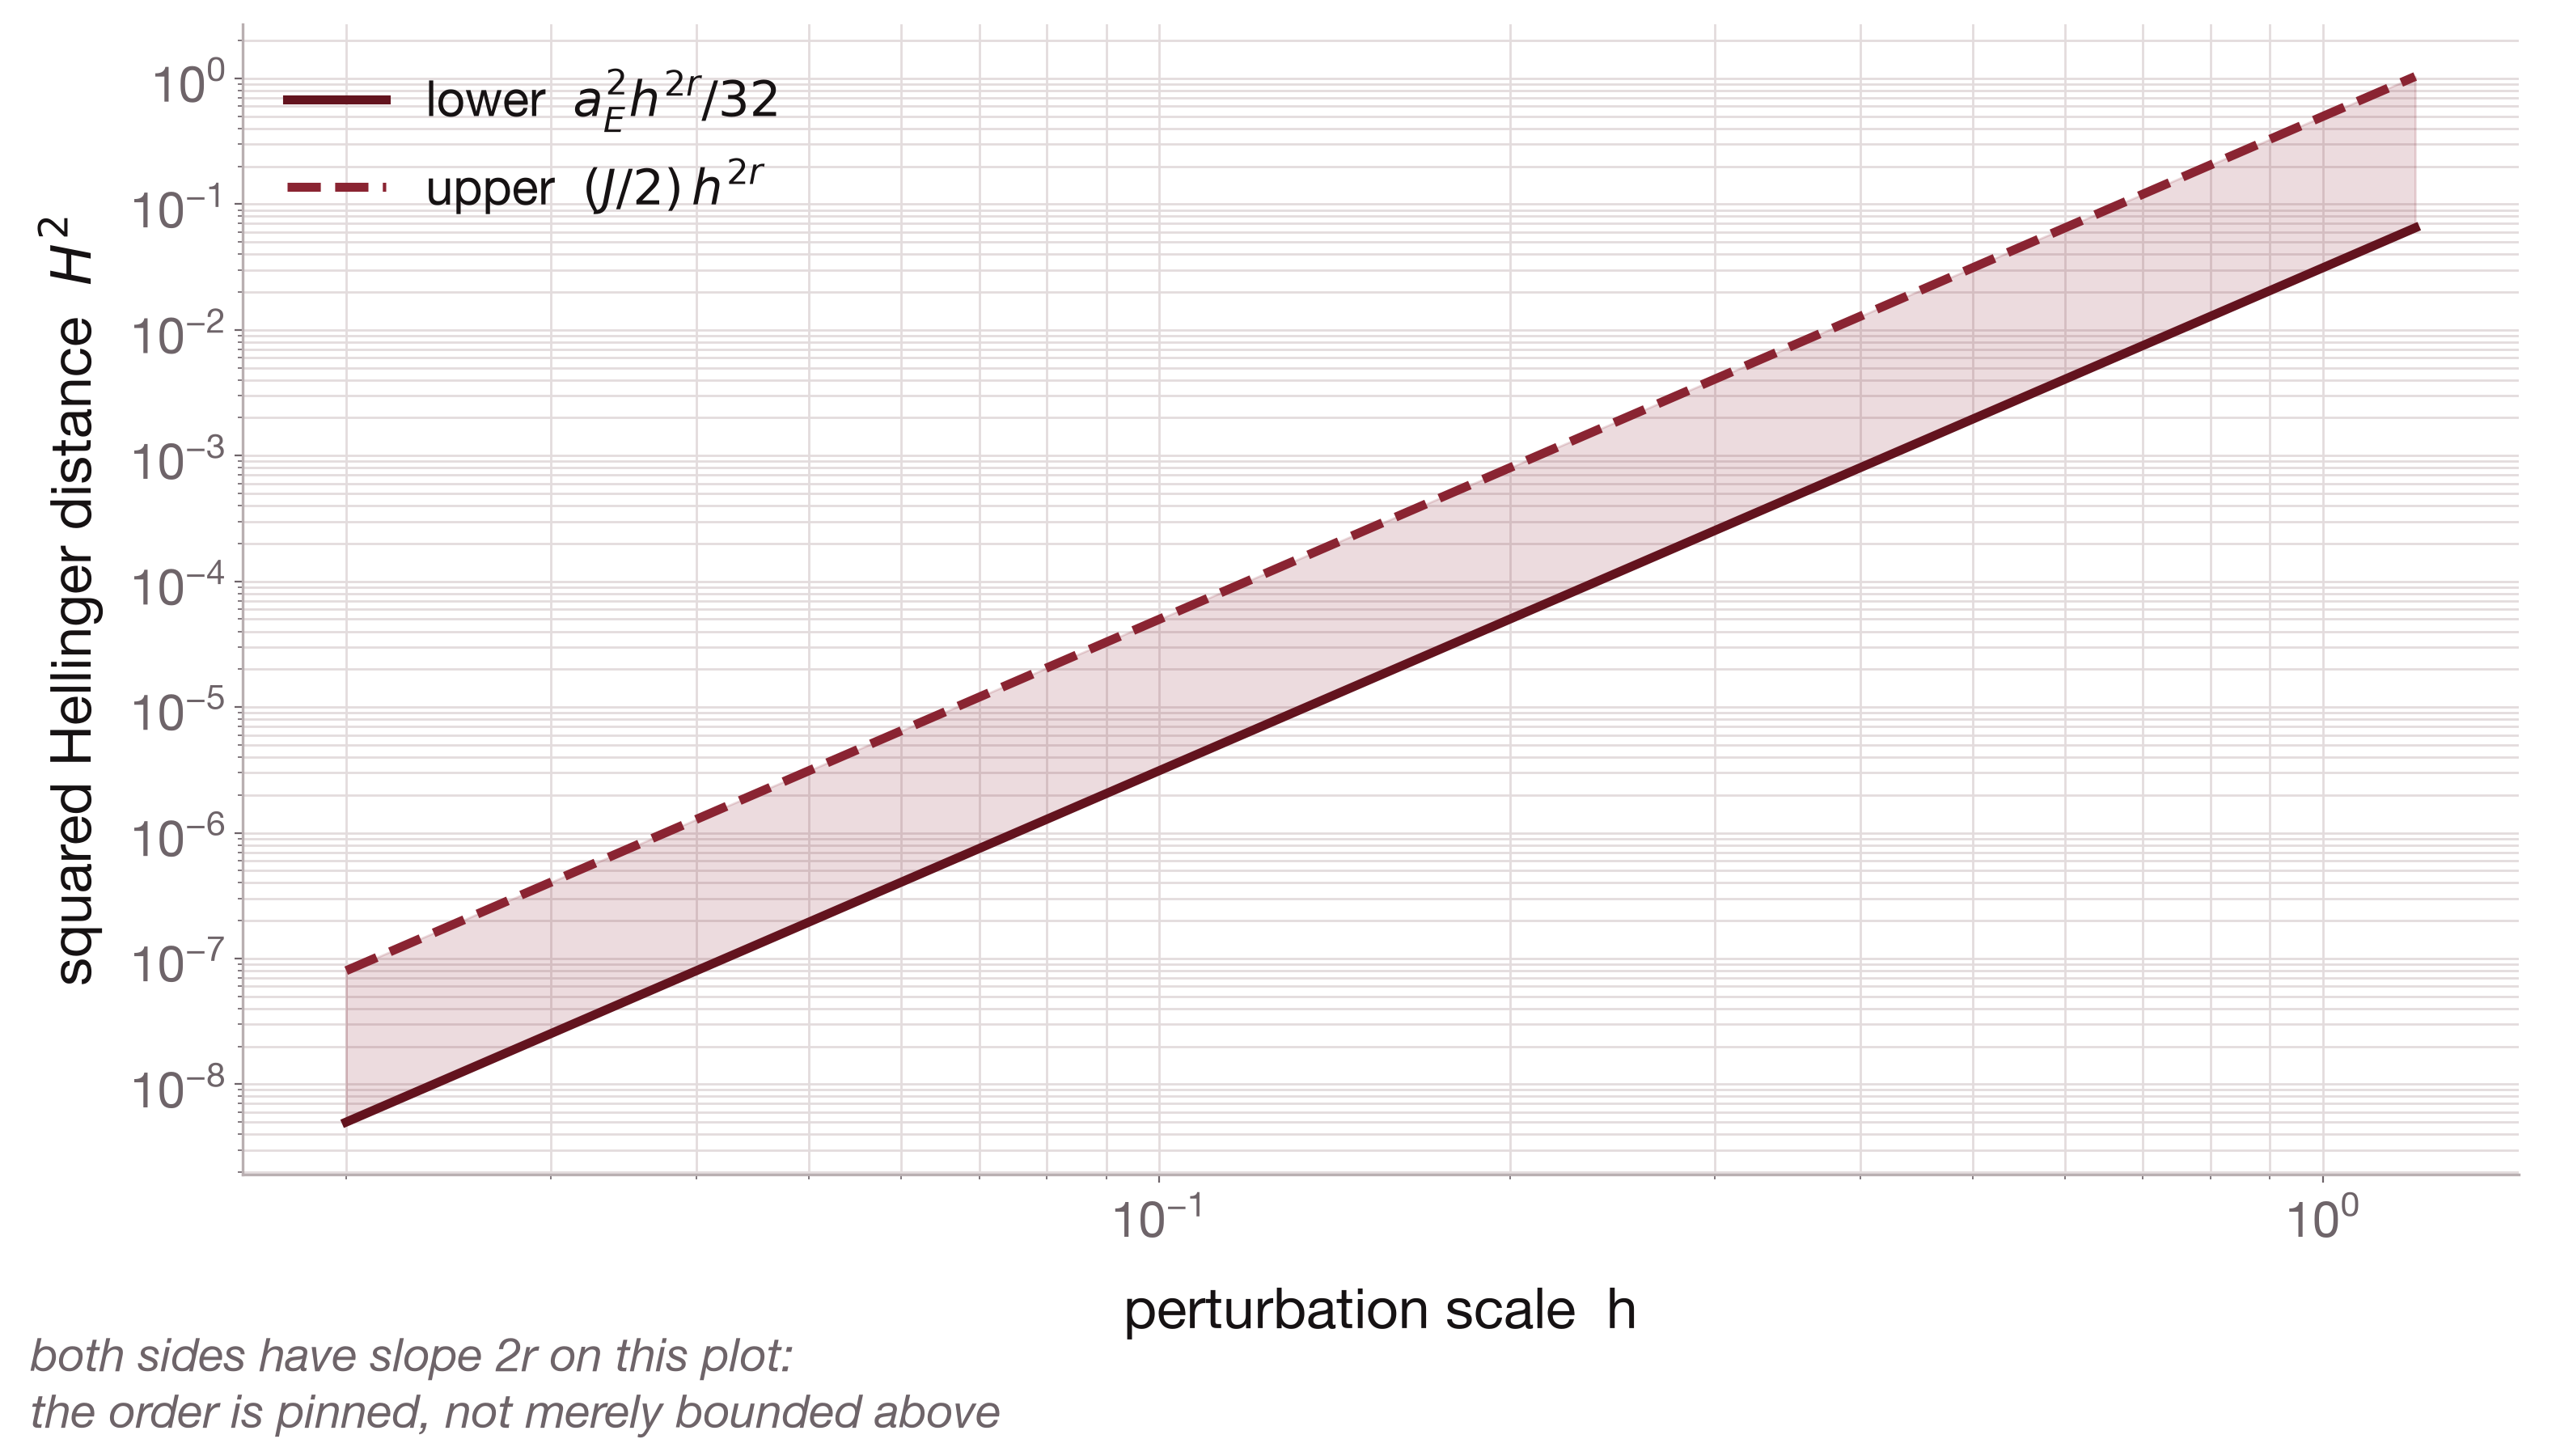
\includegraphics[width=\columnwidth]{query_fig2_sandwich.png}
\caption{The Hellinger sandwich of Theorem~\ref{thm:qy-sandwich}. Both envelopes have slope
$2r$ on this log-log plot, so the leakage order is pinned rather than merely bounded above.
The gap between them is the ratio of the two explicit constants and does not grow as
$h\downarrow0$.}
\label{fig:qy-sandwich}
\end{figure}

\subsection{From Divergence to Samples}
\label{sec:qy-samples}

\begin{lemma}[Per-sample information]
\label{lem:qy-logsandwich}
For $0\le H^{2}\le\tfrac12$,
\begin{equation}
H^{2}\;\leq\;-\log\bigl(1-H^{2}\bigr)\;\leq\;2H^{2}.
\label{eq:qy-logsandwich}
\end{equation}
\end{lemma}

\begin{proof}
The left inequality is $\log(1-u)\le-u$ on $[0,1)$. The right is $-\log(1-u)\le2u$ on
$[0,\tfrac12]$, since $u\mapsto2u+\log(1-u)$ vanishes at $0$ and has derivative
$2-1/(1-u)\ge0$ exactly there.
\end{proof}

\leanbox{\lean{log\_sandwich} in \lean{LeanQuerySampleComplexityV1}}

Lemma~\ref{lem:qy-logsandwich} transports \eqref{eq:qy-sandwich} from the Hellinger distance to the
per-sample log-affinity $L=-\log(1-H^{2})$ at the cost of a factor $2$. The factor is
tracked rather than absorbed because it is one of the two explicit constants separating
sufficiency from necessity below.

\begin{theorem}[Matching sample counts]
\label{thm:qy-samples}
Writing $\rho=1-H^{2}$ for the per-sample affinity and $\varepsilon$ for the target error,
\begin{equation}
\log\frac{1}{2\varepsilon}\;\leq\;N\,L
\qquad\Longrightarrow\qquad
\frac{\rho^{N}}{2}\;\leq\;\varepsilon .
\label{eq:qy-samples}
\end{equation}
The integer ceiling of the left-hand requirement suffices, and the corresponding necessity
count differs from it only by the factor $2$ of Lemma~\ref{lem:qy-logsandwich} and the ratio of
the two constants of Theorem~\ref{thm:qy-sandwich}.
\end{theorem}

\begin{proof}
The $N$-sample affinity between product measures tensorises to $\rho^{N}$, and the optimal
test's error probability is at most half the affinity. Requiring $\rho^{N}/2\le\varepsilon$
gives $N\log(1/\rho)\ge\log(1/2\varepsilon)$, which is the stated condition with
$L=\log(1/\rho)$. Since $N$ is an integer, its ceiling suffices; this is stated separately
because the passage from a real requirement to an integer count is exactly where an
off-by-one would hide. For necessity the same affinity bounds the error probability from
below up to a constant, so both counts scale as $h^{-2r}$ and their ratio is
$2\cdot(J/2)/(a_{E}^{2}/32)=16J/a_{E}^{2}$; the $1/(r!)^{2}$ carried by both sides of
Theorem~\ref{thm:qy-sandwich} cancels here, so the width of the window does not depend on it.
\end{proof}

\leanbox{\lean{sufficient\_count}, \lean{necessary\_count}, \lean{ceil\_suffices},
\lean{matching\_rate} in \lean{LeanQuerySampleComplexityV1}}

\noindent\emph{Supporting results in \lean{LeanQuerySampleComplexityV1}.}~These transport the sandwich to sample counts. The two logarithm bounds are what give Lemma~\ref{lem:qy-logsandwich} its factor of two, and \lean{ceil\_suffices} is stated separately because the passage from a real requirement to an integer count is exactly where an off-by-one would hide. They are reproduced as the prover has them; a further $7$ audited declarations in this module are positivity checks and measurability side conditions and are not displayed.

\noindent\textbf{S\,22}\quad\lean{matching\_rate}
{\footnotesize\[ \begin{aligned}[t]
&(\mathit{H2} \mathit{L} \mathit{cminus} \mathit{cplus} \mathit{h2r} \mathit{eps} : \mathbb{R} ),\; (\mathit{N} : \mathbb{N} ),\; (\mathit{hH0} : 0 \leq \mathit{H2}),\\
&\quad \; (\mathit{hH1} : \mathit{H2} \leq 1/2),\; (\mathit{hLdef} : \mathit{L} = -\mathit{Real}.\mathit{log} (1 - \mathit{H2})),\\
&\quad \; (\mathit{hlo} : \mathit{cminus} * \mathit{h2r} \leq \mathit{H2}),\; (\mathit{hhi} : \mathit{H2} \leq \mathit{cplus} * \mathit{h2r}),\\
&\quad \; (\mathit{heps} : 0 < \mathit{eps}),\; (\mathit{hcm} : 0 < \mathit{cminus}),\; (\mathit{hh} : 0 < \mathit{h2r}),\\
&\quad \; (\mathit{hsuff} : \mathit{Real}.\mathit{log} (1 / (2 * \mathit{eps})) \leq (\mathit{N} : \mathbb{R} ) * (\mathit{cminus} * \mathit{h2r})\\
&\quad )\\
\vdash\;&(\mathit{cminus} * \mathit{h2r} \leq \mathit{L} \wedge \mathit{L} \leq 2 * (\mathit{cplus} * \mathit{h2r})) \wedge\\
&\quad \mathit{Real}.\mathit{log} (1 / (2 * \mathit{eps})) \leq (\mathit{N} : \mathbb{R} ) * \mathit{L}
\end{aligned} \]}


``Matching'' here means matching \emph{in the exponent}, with the separating constant written
down. It does not mean the two counts coincide; a statement that the constants also match
would require sharpening both sides of Theorem~\ref{thm:qy-sandwich} and is not claimed.

\begin{theorem}[Regret window]
\label{thm:qy-regret}
With loss-geometry constants $\gamma$ and $L_{\max}$,
\begin{equation}
\frac{\gamma}{4}\,\rho^{2N}\;\leq\;R_{N}^{*}\;\leq\;\frac{L_{\max}}{2}\,\rho^{N}.
\label{eq:qy-regret}
\end{equation}
On the instance of Section~\ref{sec:qy-results}, $\gamma=\tfrac{13983}{32768}$ and
$L_{\max}=\tfrac{2401}{4096}$, both exact rationals read off the loss geometry.
\end{theorem}

\leanbox{\lean{regret\_ge\_gamma\_error}, \lean{lrt\_regret\_le},
\lean{bayes\_regret\_window} in \lean{LeanQueryRegretBridgeV1}}

\noindent\emph{Supporting results in \lean{LeanQueryRegretBridgeV1}.}~These convert an error probability into a regret window. The two loss-geometry constants enter through the inside and outside costs, and the likelihood-ratio bound supplies the upper end; the two ends carry different powers of the affinity, which is why the window widens rather than closes. They are reproduced as the prover has them; a further $3$ audited declarations in this module are positivity checks and measurability side conditions and are not displayed.

\noindent\textbf{S\,23}\quad\lean{lrt\_regret\_le}
{\footnotesize\[ \begin{aligned}[t]
&(\mathit{PA} \mathit{PB} : \mathit{H} \to \mathbb{R} ),\; (\mathit{dec} : \mathit{H} \to \mathit{Bool}),\; (\mathit{lA} \mathit{lB} : \mathit{Act} \to \mathbb{R} ),\\
&\quad \; (\mathit{aA} \mathit{aB} : \mathit{Act}),\; (\mathit{Lmax} : \mathbb{R} ),\; (\mathit{hPA} : \forall \mathit{h}, 0 \leq \mathit{PA} \mathit{h}),\\
&\quad \; (\mathit{hPB} : \forall \mathit{h}, 0 \leq \mathit{PB} \mathit{h}),\; (\mathit{hA0} : \mathit{lA} \mathit{aA} = 0),\; (\mathit{hB0} : \mathit{lB} \mathit{aB} = 0)\\
&\quad ,\; (\mathit{hAx} : \mathit{lA} \mathit{aB} \leq \mathit{Lmax}),\; (\mathit{hBx} : \mathit{lB} \mathit{aA} \leq \mathit{Lmax})\\
\vdash\;&(\textstyle\sum \mathit{h}, \mathit{PA} \mathit{h} * \mathit{lA} (\mathbf{if} \mathit{dec} \mathit{h} \mathbf{then} \mathit{aA} \mathbf{else} \mathit{aB}) + \textstyle\sum \mathit{h}, \mathit{PB} \mathit{h} * \mathit{lB} (\mathbf{if} \mathit{dec} \mathit{h}\\
&\quad \mathbf{then} \mathit{aA} \mathbf{else} \mathit{aB})) / 2 \leq \mathit{Lmax} * ((\textstyle\sum \mathit{h}, \mathit{PA} \mathit{h} * (\mathbf{if} \mathit{dec} \mathit{h} \mathbf{then} (0:\\
&\quad \mathbb{R} ) \mathbf{else} 1) + \textstyle\sum \mathit{h}, \mathit{PB} \mathit{h} * (\mathbf{if} \mathit{dec} \mathit{h} \mathbf{then} (1:\mathbb{R} ) \mathbf{else} 0)) / 2)
\end{aligned} \]}

\noindent\textbf{S\,24}\quad\lean{regret\_ge\_gamma\_error}
{\footnotesize\[ \begin{aligned}[t]
&(\mathit{PA} \mathit{PB} : \mathit{H} \to \mathbb{R} ),\; (\mathit{D} : \mathit{H} \to \mathit{Act} \to \mathbb{R} ),\; (\mathit{lA} \mathit{lB} : \mathit{Act} \to \mathbb{R}\\
&\quad ),\; (\mathit{GA} \mathit{GB} : \mathit{Finset} \mathit{Act}),\; (\mathit{gamma} : \mathbb{R} ),\; (\mathit{hPA} : \forall \mathit{h}, 0 \leq\\
&\quad \mathit{PA} \mathit{h}),\; (\mathit{hPB} : \forall \mathit{h}, 0 \leq \mathit{PB} \mathit{h}),\; (\mathit{hD} : \forall \mathit{h} \mathit{a}, 0 \leq \mathit{D} \mathit{h} \mathit{a}),\\
&\quad \; (\mathit{hDsum} : \forall \mathit{h}, \textstyle\sum \mathit{a}, \mathit{D} \mathit{h} \mathit{a} = 1),\; (\mathit{hlA} : \forall \mathit{a}, 0 \leq \mathit{lA} \mathit{a}),\\
&\quad \; (\mathit{hlB} : \forall \mathit{a}, 0 \leq \mathit{lB} \mathit{a}),\; (\mathit{hA} : \forall \mathit{a} \notin \mathit{GA}, \mathit{gamma} \leq \mathit{lA} \mathit{a}),\\
&\quad \; (\mathit{hB} : \forall \mathit{a} \notin \mathit{GB}, \mathit{gamma} \leq \mathit{lB} \mathit{a}),\; (\mathit{hdis} : \mathit{Disjoint} \mathit{GA} \mathit{GB})\\
\vdash\;&\mathit{gamma} * ((\textstyle\sum \mathit{h}, \mathit{PA} \mathit{h} * (\textstyle\sum \mathit{a} \in \mathit{GAᶜ}, \mathit{D} \mathit{h} \mathit{a}) + \textstyle\sum \mathit{h}, \mathit{PB} \mathit{h} * (1 - \textstyle\sum \mathit{a}\\
&\quad \in \mathit{GAᶜ}, \mathit{D} \mathit{h} \mathit{a})) / 2) \leq (\textstyle\sum \mathit{h}, \mathit{PA} \mathit{h} * (\textstyle\sum \mathit{a}, \mathit{D} \mathit{h} \mathit{a} * \mathit{lA} \mathit{a}) + \textstyle\sum \mathit{h},\\
&\quad \mathit{PB} \mathit{h} * (\textstyle\sum \mathit{a}, \mathit{D} \mathit{h} \mathit{a} * \mathit{lB} \mathit{a})) / 2
\end{aligned} \]}


\begin{proof}[Proof outline]
The lower side bounds regret below by the error probability times the smallest loss gap
$\gamma$, and the error probability below by a function of the affinity. The upper side uses
the likelihood-ratio test, whose error probability is at most $\rho^{N}/2$ and whose regret
is at most $L_{\max}$ times that.
\end{proof}

The two ends of \eqref{eq:qy-regret} carry $\rho^{2N}$ and $\rho^{N}$, so the window widens on a
log scale as $N$ grows. It localises regret; it does not determine it. This is stated plainly
because Section~\ref{sec:qy-results} plots measurements against a band, and a band that widens
is a weaker claim than one that closes.

\subsection{The Analytic Limit}
\label{sec:qy-limit}

A sandwich localises the normalised ratio inside an interval. It does not say the ratio
converges, and it does not identify a limit. Both are proved, and the second closes the loop
back to the crux.

\begin{theorem}[Convergence with positive limit]
\label{thm:qy-limit}
As $h\downarrow0$,
\begin{equation}
\frac{H^{2}}{h^{2r}}\;\longrightarrow\;\frac{1}{8\,(r!)^{2}}\int\frac{\Delta_{r}^{2}}{p_{0}}
\;>\;0 .
\label{eq:qy-limit}
\end{equation}
\end{theorem}

\begin{proof}[Proof outline]
Convergence is dominated convergence along $h\downarrow0$, with the integrable envelope
already constructed for the upper side of Theorem~\ref{thm:qy-sandwich} as the dominating
function. For strict positivity, the integrand $\Delta_{r}^{2}/p_{0}$ is non-negative and
integrable; a non-negative integrable function with zero integral is almost everywhere zero,
which would force $\Delta_{r}\equiv0$ almost everywhere, contradicting
Theorem~\ref{thm:qy-nonvanish}.
\end{proof}

\leanbox{\lean{ratio\_tendsto\_of\_dominated}, \lean{hellinger\_ratio\_tendsto},
\lean{limit\_pos\_of\_ae\_ne\_zero}, \lean{eventually\_pos\_of\_limit\_pos} in
\lean{LeanQueryAnalyticLimitV1}}
\TODOPAR{Where this module stops. \lean{hellinger\_ratio\_tendsto} takes five
hypotheses---\lean{hmeas}, \lean{hdom} ($\lVert F_{h}\rVert\le\mathit{bound}$), \lean{hint}
($\mathit{bound}$ integrable), \lean{hptw} (the pointwise limit
$F_{h}\to\Delta_{r}^{2}/4p_{0}$), and \lean{hH2} (the Hellinger identity
$H^{2}(h)=\tfrac12\int F_{h}$)---and concludes the limit. It is therefore a dominated
-convergence wrapper: it says the interchange is legitimate \emph{given} domination, the
pointwise limit and the identity, and none of those three is established here for the
normalised observation laws this paper is actually about. \lean{ratio\_tendsto\_of\_dominated}
is the same shape one level down. What is missing is an instantiation: exhibit the envelope,
prove the pointwise convergence from the mixture, and derive the identity from the
normalisation, so that Theorem~\ref{thm:qy-limit} rests on the model rather than on three
assumptions about it. Until then the paper should say the limit is proved \emph{modulo} those
three inputs, which is weaker than it currently reads.}

Theorem~\ref{thm:qy-limit} upgrades the result from ``the rate is $h^{2r}$ up to constants'' to
``the leading constant exists and is positive''. Positivity of the limit is \emph{equivalent}
to non-vanishing of $\Delta_{r}$, so the crux step is used twice: once to obtain a lower
envelope, and once to certify that the envelope is not vacuous.

\subsection{Determining the Order of a Candidate Query}
\label{sec:qy-procedure}

The results are worth little to a designer who cannot tell, given a candidate measurement,
what order it has. The proofs supply a finite procedure.

\begin{algorithm}[htbp]
\caption{Leakage order of a candidate measurement}
\label{alg:qy-order}
\begin{algorithmic}[1]
\STATE Collect the distinct levels $v$ taken by $f_{W}$, with the aggregate weight at each.
\STATE $j\leftarrow0$.
\REPEAT
  \STATE Form the level coefficients $M_{j}(v)$ by grouping the order-$j$ terms of the
         expansion of \eqref{eq:qy-mixture}; by Theorem~\ref{thm:qy-sumswap} this is a finite
         exact sum.
  \IF{the $M_{j}(v)$ cancel across levels}
    \STATE $j\leftarrow j+1$.
  \ENDIF
\UNTIL{cancellation fails}
\STATE Let $v^{*}$ be the largest level with $M_{j}(v^{*})\neq0$.
\IF{$v^{*}$ is strictly largest}
  \STATE \textbf{return} $r=j$ \COMMENT{certified by Theorem~\ref{thm:qy-nonvanish}}
\ELSE
  \STATE \textbf{return} \textsc{undetermined} \COMMENT{ties are outside the theorem}
\ENDIF
\end{algorithmic}
\end{algorithm}

Two properties matter. The procedure never simulates the measurement: steps 1--8 are exact
arithmetic on the mixture data, so candidate queries can be compared before any data are
collected. And step~11 has an explicit failure mode rather than a silent one, which is the
honest output given that Theorem~\ref{thm:qy-nonvanish} does not cover ties.


\section{Experimental Design}

\subsection{Deciding Without Identifying: An Exact Minimax Law}
\label{sec:sp-expdesign}

\subsection{Experimental Objectives}

Theorem~\ref{thm:sp-separation} states the decide side exactly, so no experiment bears on it. The
computation has three objectives. The first is to evaluate both thresholds on a grid so that
the ratio, which the theorem does not compute, can be read off. The second is scope: twelve
cells at one value of $P$ cannot distinguish a law from a coincidence, and the grid below is
widened until the growth in $K$ can be fitted rather than asserted. The third is the one that
can actually fail. Equation~\eqref{eq:sp-recover} is an inclusion--exclusion identity over events
that are \emph{not} independent---the classes compete for the same $N$ observations---and it
is derived rather than measured. Experiment~E2 simulates the process it is derived for and
compares.

\subsection{Setup}

The grid is
\begin{align*}
K &\in \{1,2,3,4,6,8,12,16,24,32,48,\\
  &\qquad 64,96,128,192,256,384,512,768,1024\},\\
P &\in \{\tfrac1{20},\tfrac1{10},\tfrac15,\tfrac14,\tfrac13,\tfrac12,\tfrac23,\tfrac34,\tfrac9{10}\},
\end{align*}
and $\varepsilon$ runs from $\tfrac1{10}$ down to $10^{-6}$, giving $1{,}080$ cells on the
model $a_{i}=b_{i}=1$, $p_{i}=P/K$.

The recovery sum alternates in sign with binomial weights, so it loses roughly $K$ bits to
cancellation and cannot be evaluated in double precision anywhere near the top of this grid:
at $K=128$ the largest term already exceeds the answer by about eighteen orders of magnitude.
The working precision is therefore set from $K$ itself, at
$120+\lceil K\log_{10}2\rceil+40$ significant digits---$469$ at $K=1024$---and checked
against exact rational arithmetic wherever the exact computation is affordable. A fixed
precision would have returned noise at the largest sizes rather than an answer.

\begin{algorithm}[htbp]
\caption{The two thresholds, at a precision set from $K$}
\label{alg:sp-threshold}
\begin{algorithmic}[1]
\REQUIRE class count $K$, per-class resolution probability $P$, tolerance $\varepsilon$
\ENSURE the least $N$ meeting $\varepsilon$ for deciding and for recovering
\STATE working precision $\leftarrow 120+\lceil K\log_{10}2\rceil+40$ significant digits
       \COMMENT{the recovery sum alternates with binomial weights and loses about $K$ bits;
       a fixed precision returns noise at the top of the grid}
\STATE $R_{\mathrm{dec}}(N)\leftarrow\tfrac12(1-P)^{N}$ \COMMENT{exact rationals; $K$ does
       not appear}
\STATE $R_{\mathrm{rec}}(N)\leftarrow1-\sum_{k=0}^{K}\binom{K}{k}\bigl(-\tfrac12\bigr)^{k}
       \bigl(1-\tfrac{kP}{K}\bigr)^{N}$
\FOR{each of the two risks}
  \STATE double $N$ from $1$ until the risk falls below $\varepsilon$, then bisect
         \COMMENT{a true threshold, not a rounded logarithm}
\ENDFOR
\STATE \textbf{self-check:} $R_{\mathrm{rec}}$ at $K=1$ must equal $R_{\mathrm{dec}}$ in
       rational arithmetic; the high-precision and exact evaluations must agree; and
       $\tfrac12\Pr(U>0)\le R_{\mathrm{rec}}\le\Pr(U>0)$ must hold
\end{algorithmic}
\end{algorithm}

\subsection{E2: The Recovery Identity Against the Process}
\label{sec:sp-e2}

Each observation picks a class uniformly and resolves it with probability $P$; after $N$ of
them, every class still unresolved is guessed with a fair coin. The quantity to measure is
therefore $\mathbb{E}[2^{-U}]$, where $U$ counts the unresolved classes---not
$\Pr(U=0)$, because a report can be correct by luck---and that expectation is exactly
$1-R_{\mathrm{rec}}$. Two hundred cells are simulated at the recovery threshold itself, with up to
$400{,}000$ replications each---traded against the horizon, since a long horizon costs
proportionally more per replication---and the standard error is retained per cell.

\subsection{Metrics}

For each cell: the least $N$ with $\tfrac12(1-P)^{N}\le\varepsilon$; the least $N$ with
\eqref{eq:sp-recover} at most $\varepsilon$; their ratio; and both risks evaluated at the
\emph{decide} count, which shows what a recovery-based procedure would still be carrying at
the moment a decision is already safe. Across cells: whether the recovery threshold is
monotone in $K$, and the constant in the coupon-collector reading
$N_{\mathrm{rec}}\approx c\,(K/P)(\ln K+\ln\tfrac1\varepsilon)$ fitted per $(P,\varepsilon)$.
For E2: the measured $\mathbb{E}[2^{-U}]$ against the identity, as a $z$-score in units of its
own standard error.

\subsection{Statistical Reporting}

The threshold counts are obtained by bisection over exact evaluations rather than by taking a
logarithm and rounding, so the integers are true thresholds rather than approximations. Three
self-checks run before any sweep result is reported, and the run refuses to report if any
fails: the recovery risk at $K=1$ must equal the decide risk \emph{exactly} in rational
arithmetic, which it does at every cell tested; the high-precision and exact-rational
evaluations must agree, and they agree to the last digit; and the sandwich
$\tfrac12\Pr(U>0)\le R_{\mathrm{rec}}\le\Pr(U>0)$ must hold, which it does everywhere. Only
E2 involves sampling, and it is reported with its standard error; no difference below twice
that error is described as an effect.

One thing recorded here must not be read as a finding. The decide threshold's independence of
$K$ is structural, not measured: the proved expression \eqref{eq:sp-decide} contains no $K$, so
the flat lines in Figure~\ref{fig:sp-counts} restate the theorem rather than confirm it. What is
measured is the growth of the recovery threshold beside it.


\subsection{The Admissible Query Sets the Leakage Order}
\label{sec:qy-expdesign}

\subsection{Experimental Objectives}

The theorems are proved, so the simulation cannot strengthen them. It has three objectives.
The first is to check that the chain from Theorem~\ref{thm:qy-sandwich} through
Theorem~\ref{thm:qy-regret} is arithmetically consistent, which a slip in any constant would
break. The second is to measure the quantity the theorems predict but do not compute: how
much the sample requirement changes when only the admissible measurement changes. The third
is generalisation. Theorem~\ref{thm:qy-sandwich} pins the exponent at $2r$ for every instance in
its hypotheses, and a single pair of worlds cannot distinguish a law from a coincidence;
Experiment~E2 therefore asks whether the exponent is $2r$ on two hundred independently drawn
instances, at three different orders.

\subsection{Setup}

Two admissible measurements of the \emph{same} pair of worlds were simulated at $h=0.6$ with
$4000$ repetitions per world: a normalised measurement of leakage order $2$ and a normalised
measurement of leakage order $1$. The worlds $f_{0},f_{1}$, the noise scale $\sigma$ and the
perturbation scale $h$ are identical across the two runs; only $g$ differs.

\subsection{E2: The Exponent Across Instances and Orders}
\label{sec:qy-e2}

\emph{Why the instance must carry two worlds.} An earlier version of this experiment drew $g$
at random around a single world and obtained leakage order $1$ on every instance, which tests
nothing. A second version tried to force higher orders by requiring the weighted level moments
$\sum_{x\in\text{level}}\pi_{x}g(x)^{j}$ to vanish below the order. That is impossible for
$j=2$: the weights are positive, so the moment is a sum of non-negative terms and vanishes
only when $g$ does. Both failures came from modelling one world and a perturbation, whereas
Theorem~\ref{thm:qy-cancel} is a statement about \emph{two} worlds sharing a level set---the
quantities that must agree below the order are $M^{(0)}_{j}(v)$ and $M^{(1)}_{j}(v)$, and
their equality is a difference of two positive sums rather than the vanishing of one. Order
three is unreachable in the first model and routine in the second, and recording this is the
difference between an experiment that can fail and one that cannot.

\emph{Instances.} Two hundred instances are drawn from declared ranges: two to four levels,
four to six indices per level, level values drawn without replacement from
$\{-3,\dots,3\}$, $\sigma\sim\mathrm{Unif}[0.7,1.5]$ and weights Dirichlet. World~$1$ is
world~$0$ with a block of indices exchanged between two levels at equal weight, which
preserves every level's mass exactly, so the two worlds are identical at $h=0$ and the
leakage order is well posed.

\emph{Designing the order.} On the exchanged block, $g$ takes the values of a
Prouhet--Thue--Morse pair: splitting $\{0,\dots,2^{r}-1\}$ by the parity of the binary digit
sum yields two sets whose $j$-th power sums agree for every $j<r$ and differ at $j=r$. The
construction is invariant under the affine maps $u\mapsto\alpha u+\beta$, so scale and offset
are randomised per instance without disturbing the order. Off the block, $g$ is drawn at
random and cancels identically, because those indices sit in the same level in both worlds.
Designed orders $r=1,2,3$ are used.

\begin{algorithm}[htbp]
\caption{An instance with a designed leakage order $r$}
\label{alg:qy-instance}
\begin{algorithmic}[1]
\REQUIRE order $r$, level count, level size, noise scale $\sigma$
\ENSURE two worlds sharing a level set with equal level masses, and a perturbation $g$ whose
        leakage order is $r$
\STATE $A\leftarrow\{k<2^{r}:\text{binary digit sum of }k\text{ even}\}$,
       $B\leftarrow\{k<2^{r}:\text{odd}\}$
       \COMMENT{Prouhet: $\sum_{A}k^{\,\ell}=\sum_{B}k^{\,\ell}$ for every $\ell<r$, and
       they differ at $\ell=r$}
\STATE normalise $A,B$ to $[0,1]$ \COMMENT{the identity is affine-invariant; the raw values
       reach $2^{r}-1$ and would push mixture components out of any fixed quadrature window}
\STATE choose two levels and a block of $|A|$ indices in each; give every block index the
       same weight, so exchanging the blocks preserves each level's mass exactly
\STATE $g\leftarrow\alpha A+\beta$ on the first block, $\alpha B+\beta$ on the second, with
       $\alpha,\beta$ drawn; draw $g$ at random off the block
       \COMMENT{off-block indices sit in the same level in both worlds and cancel}
\STATE world~$1$ is world~$0$ with the two blocks exchanged
\STATE \textbf{verify:} recompute $M^{(0)}_{\ell}(v)-M^{(1)}_{\ell}(v)$ for
       $\ell=1,2,\dots$ and report the least $\ell$ at which it is non-zero; a tie at the top
       level is reported as undetermined rather than counted
\end{algorithmic}
\end{algorithm}

\emph{Verification, not assumption.} The order is then recomputed from the level coefficients
by the procedure of Section~\ref{sec:qy-procedure} and compared with the designed one; a cell
whose top level is tied is reported as undetermined rather than counted. A self-check runs
before the sweep and must pass for it to be reported at all: level masses must agree to
machine precision, the verified order must equal the designed order on every check instance,
and $H^{2}$ must be stable between the working quadrature grid and one twice as fine and
twice as wide.

\emph{Measurement.} $H^{2}$ between the two worlds is computed by quadrature on a
fourteen-point grid $h=0.5\cdot0.6^{i}$ reaching $6.5\times10^{-4}$. The exponent is
estimated by least squares on the asymptotic tail only, $h\le0.023$; the full-grid fit is
reported next to it rather than the pre-asymptotic points being dropped silently, because the
difference between the two is itself informative about where the asymptotic regime begins.

\subsection{E3: Orders Four and Five, and the Arithmetic Floor}
\label{sec:qy-e3}

Theorem~\ref{thm:qy-sandwich} is stated for every $r$, so the sweep should not stop at three. It
cannot simply continue on the same grid, for a reason worth stating rather than discovering.
$H^{2}$ falls like $h^{2r}$, so at order five and $h=6.5\times10^{-4}$ the true value is
about $10^{-32}$, while it is computed as an integral of
$(\sqrt{p}-\sqrt{q})^{2}$ with $p$ and $q$ both of order one. Double precision resolves their
difference to about $10^{-16}$ in absolute terms, so everything below roughly $10^{-24}$ in
$H^{2}$ is rounding, and a slope fitted through it would be a fit to arithmetic noise.

The grid is therefore chosen per order: it runs from $h=0.5$ down to where the predicted
$H^{2}$ reaches $10^{-18}$, which keeps every evaluated value inside the range double
precision represents while still spanning enough decades to fit a slope. The floor is
declared in advance, not tuned after seeing the answer, and each cell carries a reliability
flag---the coefficient of determination of its tail fit---so a cell that drifts into the
noise is visible rather than averaged in.

Two adjustments to the construction were needed. The Prouhet block has $2^{r-1}$ cells on
each side, so orders four and five need eight and sixteen cells per level rather than the
main sweep's four to six. And the raw Prouhet values run up to $2^{r}-1$, which is $31$ at
order five; scaled by $h$ and by the random $\alpha$, they would push mixture components
outside any fixed quadrature window, which a first run duly did---the quadrature self-check
reported an eighteen per cent disagreement. The identity is invariant under affine maps, so
the block is normalised to $[0,1]$ and $\alpha,\beta$ supply the randomisation; the
disagreement fell to $3\times10^{-11}$.

\subsection{Baselines and Comparison}

The comparison is between the two measurements, not against an external baseline: the point
is to isolate the effect of the measurement while holding everything else fixed. The
per-sample $H^{2}$ is computed directly from \eqref{eq:qy-mixture} in both cases rather than
through the sandwich, so the reported divergences are properties of the measurements and not
consequences of Theorem~\ref{thm:qy-sandwich}.

\subsection{Metrics}

The reported quantities are the per-sample $H^{2}$ and $L$, the required sample count $N$
from Theorem~\ref{thm:qy-samples}, the measured Bayes regret under an equal prior, a percentile
bootstrap interval, and the two ends of the window \eqref{eq:qy-regret}.

\subsection{Statistical Reporting}

Uncertainty is a percentile bootstrap over the $8000$ per-repetition regrets with $2000$
resamples. Experiment~E2 contains no sampling in its main measurement---$H^{2}$ is a
quadrature of a density, not an average over draws---so it carries no confidence interval;
what it carries instead is the quadrature self-check, which bounds the only error it can have.
Where E2 does simulate, to confirm that the sample count derived from $H^{2}$ achieves the
target error, three independent seeds of $2000$ repetitions per world are used and the
seed-to-seed spread is retained. The window endpoints are computed in exact rational arithmetic where the loss
geometry permits ($\gamma=13983/32768$, $L_{\max}=2401/4096$) and in double precision
otherwise. Evidence classes are kept apart: \PROVED{}, \CERT{} and \NUM{} are distinguished
throughout and no \NUM{} result supports a \PROVED{} one.


\section{Formal Verification}

\subsection{Deciding Without Identifying: An Exact Minimax Law}
\label{sec:sp-verification}

\subsection{Acceptance Contract}

A module counts as accepted only when all six of the following hold: the compiler exits zero
with no errors; the source hash is unchanged \emph{across} the compile, so the file checked is
the file on disk; the compiled artifact is newer than its source; at least one
\texttt{\#print axioms} directive is present; the axiom set of every audited declaration lies
within $\{\textsf{propext},\textsf{Classical.choice},\textsf{Quot.sound}\}$; and no
\texttt{sorry} appears anywhere in the file.

This contract is shared with the other papers of the programme and is reproduced verbatim in
each, so that no paper's evidence claim has to be read against a different standard; the
wording is common and the counts in this section are not. The contract is stated in full
because each clause excludes a specific way of appearing verified without being so. The hash check across the compile excludes editing a file after
checking it; the artifact-newer check excludes a stale \texttt{.olean}; and the axiom audit is
a \emph{whitelist} rather than a blacklist, so an axiom introduced by a decision procedure
outside the kernel is rejected by name mismatch rather than needing to be anticipated.

\subsection{Evidence per Step}

\begin{table}[htbp]
\caption{Evidence per step. All cited declarations are axiom-audited.}
\label{tab:sp-inventory}
\centering\footnotesize\setlength{\tabcolsep}{3pt}
\begin{tabular}{@{}llr@{}}
\toprule
Step & Module & Aud. \\
\midrule
Sampling, Thm~\ref{thm:sp-sampling}      & \lean{LeanSupportSamplingLawV1}        & 9 \\
Decoder, Thm~\ref{thm:sp-equivariant}    & \lean{LeanSupportEquivariantDecoderV1} & 4 \\
Factorisation, Thm~\ref{thm:sp-factor}   & \lean{LeanSupportMinimaxLowerV1}       & 6 \\
Optimality, Thm~\ref{thm:sp-optimal}     & \lean{LeanSupportMinimaxLowerV1}       & 6 \\
Minimax, Thm~\ref{thm:sp-minimax}        & \lean{LeanSupportMinimaxLowerV1}       & 6 \\
Three worlds, Thm~\ref{thm:sp-threeworld}& \lean{LeanSupportThreeWorldWitnessV1}  & 5 \\
Separation, Thm~\ref{thm:sp-separation}  & \lean{LeanSupportDecideRecoverV1}      & 11 \\
\bottomrule
\end{tabular}
\end{table}

\subsection{Scope of the Formalisation}

The Support strand contains $50$ Lean source files with $870$ theorem and lemma statements,
of which $21$ modules carry an acceptance receipt covering $183$ audited declarations. Across
the programme: $762$ files, $7{,}199$ statements, $111$ accepted modules, $857$ audited
declarations.

Two formulations were withdrawn under the prover. The original minimax statement took constant
risk as a premise and contained no quantifier over rules anywhere in its statement; written out
formally, the gap was unmissable, since the conclusion mentions one rule and one prior and
there is no second rule to compare against. And the sampling law initially assumed independence
between classes in order to factor an expectation, which is unnecessary---linearity suffices
for the sum actually needed---and removing it also removed a hypothesis from the recovery law.
Every audited statement of every module this paper cites is displayed in Section~\ref{sec:sp-setting}, attached to the step that uses it; only positivity checks and measurability side conditions are omitted, and their count is given at each block. The strand contains a further $17$ accepted modules carrying $153$ audited declarations that no step of this paper uses; they belong to other results of the programme. Appendix~\ref{app:sp-inventory} reproduces the complete chain: all $183$ audited statements of the strand across its $21$ accepted modules, grouped by module.


\subsection{The Admissible Query Sets the Leakage Order}
\label{sec:qy-verification}

\subsection{Acceptance Contract}

A module counts as accepted only when all six of the following hold: the compiler exits zero
with no errors; the source hash is unchanged \emph{across} the compile, so the file checked is
the file on disk; the compiled artifact is newer than its source; at least one
\texttt{\#print axioms} directive is present; the axiom set of every audited declaration lies
within $\{\textsf{propext},\textsf{Classical.choice},\textsf{Quot.sound}\}$; and no
\texttt{sorry} appears anywhere in the file.

This contract is shared with the other papers of the programme and is reproduced verbatim in
each, so that no paper's evidence claim has to be read against a different standard; the
wording is common and the counts in this section are not. The contract is stated in full
because each clause excludes a specific way of appearing verified without being so. The hash check across the compile excludes editing a file after
checking it; the artifact-newer check excludes a stale \texttt{.olean}; and the axiom audit is
a \emph{whitelist} rather than a blacklist, so an axiom introduced by a decision procedure
outside the kernel is rejected by name mismatch rather than needing to be anticipated.

\subsection{Evidence per Step}

\begin{table}[htbp]
\caption{Evidence per step. All cited declarations are axiom-audited.}
\label{tab:qy-inventory}
\centering\footnotesize\setlength{\tabcolsep}{3pt}
\begin{tabular}{@{}llr@{}}
\toprule
Step & Module & Aud. \\
\midrule
Derivatives, Thm~\ref{thm:qy-hermite}     & \lean{LeanQueryGaussianLevelV1}     & 13 \\
Sum rule, Thm~\ref{thm:qy-sumswap}        & \lean{LeanQueryMixtureDerivativeV1} &  5 \\
Cancellation, Thm~\ref{thm:qy-cancel}     & \lean{LeanQueryMixtureDerivativeV1} &  5 \\
Non-vanishing, Thm~\ref{thm:qy-nonvanish} & \lean{LeanQueryGaussianLevelV1}     & 18 \\
Sandwich, Thm~\ref{thm:qy-sandwich}       & \lean{LeanQueryHellingerIntervalV1} & 14 \\
Samples, Thm~\ref{thm:qy-samples}         & \lean{LeanQuerySampleComplexityV1}  &  8 \\
Regret, Thm~\ref{thm:qy-regret}           & \lean{LeanQueryRegretBridgeV1}      &  5 \\
Limit, Thm~\ref{thm:qy-limit}             & \lean{LeanQueryAnalyticLimitV1}     &  4 \\
\bottomrule
\end{tabular}
\end{table}

\subsection{Scope of the Formalisation}

The Query strand contains $27$ Lean source files with $167$ theorem and lemma statements,
of which $13$ modules carry an acceptance receipt covering $87$ audited declarations. Across
the programme: $762$ files, $7{,}199$ statements, $111$ accepted modules, $857$ audited
declarations.

Two defects in earlier drafts were found by the prover rather than by reading. The lower
constant in Theorem~\ref{thm:qy-sandwich} was initially $16$, produced by bounding
$(\sqrt{p}+\sqrt{q})^{2}$ by $p+q$, which is false; the error is invisible in a numerical
check because the resulting envelope is still valid wherever slack absorbs the factor. And the
smoothness hypothesis in Theorem~\ref{thm:qy-sumswap} was initially assumed rather than derived,
which would have left the paper's main technical contribution resting on an unproved side
condition. Every audited statement of every module this paper cites is displayed in Section~\ref{sec:qy-setting}, attached to the step that uses it; only positivity checks and measurability side conditions are omitted, and their count is given at each block. The strand contains a further $8$ accepted modules carrying $49$ audited declarations that no step of this paper uses; they belong to other results of the programme. Appendix~\ref{app:qy-inventory} reproduces the complete chain: all $87$ audited statements of the strand across its $13$ accepted modules, grouped by module.


\section{Results}

\subsection{Deciding Without Identifying: An Exact Minimax Law}
\label{sec:sp-results}

\subsection{Reporting Protocol}

All twelve cells are reported with no exclusions.

\subsection{Deciding Is Flat in $K$; Recovering Is Not}

At $P=\tfrac12$ and $\varepsilon=\tfrac{1}{100}$, deciding takes $6$ samples whether there is
one class or thirty-two. Recovering takes $6$ at $K=1$, $17$ at $K=2$, and more as $K$ grows.
Both columns are exact integers obtained by inverting closed forms.

The risk columns say the same thing from the other side. At the moment the decide risk has
reached $\tfrac{1}{128}$, the recovery risk is still $\tfrac{713}{4096}$ at $K=2$---about
twenty-two times larger---and the gap widens with $K$. An experimenter who stops when they can
decide is done; one who stops when they can identify is still far from it.

\begin{table*}[t]
\caption{Exact sample counts for deciding and for recovering, on the model
$a_{i}=b_{i}=1$, $p_{i}=P/K$ with total unsafe mass $P$ held fixed. Every entry is exact
rational arithmetic; nothing is simulated. The decide column does not move with $K$---the
same count serves $K=1$ and $K=64$ at a given $(P,\varepsilon)$, which is
\eqref{eq:sp-decide}---while the recover column grows, and with it the ratio. The last two
columns are the two risks evaluated at the \emph{decide} count, so they show directly what a
recovery-based procedure would still be carrying at the moment a decision is already safe.
The recovery law is an inclusion--exclusion identity and assumes no independence between
classes.}
\label{tab:sp-separation}
\centering
\footnotesize
\setlength{\tabcolsep}{6pt}
\begin{tabular}{@{}rrrrrrrr@{}}
\toprule
$K$ & $P$ & $\varepsilon$ & $N_{\mathrm{decide}}$ & $N_{\mathrm{recover}}$ &
ratio & $R_{\mathrm{dec}}$ at $N_{\mathrm{decide}}$ & $R_{\mathrm{rec}}$ at $N_{\mathrm{decide}}$ \\
\midrule
1 & $\frac{1}{2}$ & $\frac{1}{10}$ & 3 & 3 & 1.000 & $\frac{1}{16}$ & $\frac{1}{16}$ \\
1 & $\frac{1}{2}$ & $\frac{1}{100}$ & 6 & 6 & 1.000 & $\frac{1}{128}$ & $\frac{1}{128}$ \\
2 & $\frac{1}{2}$ & $\frac{1}{10}$ & 3 & 8 & 2.667 & $\frac{1}{16}$ & $\frac{25}{64}$ \\
2 & $\frac{1}{2}$ & $\frac{1}{100}$ & 6 & 17 & 2.833 & $\frac{1}{128}$ & $\frac{713}{4096}$ \\
4 & $\frac{1}{2}$ & $\frac{1}{10}$ & 3 & 23 & 7.667 & $\frac{1}{16}$ & $\frac{841}{1024}$ \\
4 & $\frac{1}{2}$ & $\frac{1}{100}$ & 6 & 40 & 6.667 & $\frac{1}{128}$ & $\frac{345741}{524288}$ \\
8 & $\frac{1}{2}$ & $\frac{1}{10}$ & 3 & 57 & 19.000 & $\frac{1}{16}$ & $\frac{64741}{65536}$ \\
8 & $\frac{1}{2}$ & $\frac{1}{100}$ & 6 & 93 & 15.500 & $\frac{1}{128}$ & $\frac{260394461}{268435456}$ \\
16 & $\frac{1}{2}$ & $\frac{1}{10}$ & 3 & 137 & 45.667 & $\frac{1}{16}$ & $\frac{67105549}{67108864}$ \\
16 & $\frac{1}{2}$ & $\frac{1}{100}$ & 6 & 211 & 35.167 & $\frac{1}{128}$ & $\frac{2198711433501}{2199023255552}$ \\
32 & $\frac{1}{2}$ & $\frac{1}{10}$ & 3 & 320 & 106.667 & $\frac{1}{16}$ & $\frac{17592186030877}{17592186044416}$ \\
32 & $\frac{1}{2}$ & $\frac{1}{100}$ & 6 & 469 & 78.167 & $\frac{1}{128}$ & $\frac{4611686007394094621}{4611686018427387904}$ \\
\bottomrule
\end{tabular}
\end{table*}


The reason the decide count does not move is visible in \eqref{eq:sp-decide}: $K$ does not appear.
A decision is correct as soon as the named tip is safe, and whether it is safe is settled
inside a single class. A recovery must resolve every class.

\subsection{The Separation Over the Whole Grid}

Figure~\ref{fig:sp-counts} puts the two thresholds on one pair of axes over ten doublings of
$K$ and four values of $P$. The decide lines are flat by construction---$K$ does not appear in
\eqref{eq:sp-decide}---while the recover curves climb steadily on a logarithmic $K$ axis. The
ratio is what an experimenter feels: at $P=\tfrac12$ and $\varepsilon=\tfrac1{100}$ recovery
costs the same $6$ samples as deciding when there is one class, $17$ at two classes, and
$22{,}192$ at a thousand and twenty-four---a factor of $3{,}699$. At $P=\tfrac1{10}$ the same
comparison runs from $38$ to $110{,}981$. The separation is not a constant overhead that a
larger budget absorbs; it widens without bound. \NUM{}

The growth has a shape, and it is the coupon-collector one. Fitting
$N_{\mathrm{rec}}\approx c\,(K/P)(\ln K+\ln\tfrac1\varepsilon)$ over each of the $54$
$(P,\varepsilon)$ slices gives $c$ between $0.916$ and $0.966$ with $R^{2}$ at least
$0.99996$ in every slice. The scale quoted for orientation in Section~\ref{sec:sp-separation} is
therefore the right one, with a constant slightly below one; the largest relative departure,
$0.53$, is at the smallest $K$, where an asymptotic form has no reason to hold. \NUM{}

\subsection{The Recovery Identity Against the Process It Describes}

Equation~\eqref{eq:sp-recover} is the part of the separation that could be wrong without anyone
noticing, because it is an inclusion--exclusion over dependent events and is derived rather
than measured. Experiment~E2 simulates the process and compares. Over $200$ cells at the
recovery threshold itself, the measured $\mathbb{E}[2^{-U}]$ differs from the identity by at
most $0.0043$ in absolute terms and by at most $2.98$ standard errors, which over two hundred
cells is what the null predicts---about half a cell beyond $2.98$ is expected, and one is
seen.
Figure~\ref{fig:sp-identity} shows every cell against the diagonal. \NUM{}

Two exact checks sit behind that. The identity at $K=1$ reduces to the decide risk, in
rational arithmetic, at every cell tested---which is the only point where the two sides of the
separation must agree, and they do. And the $240$-digit evaluation agrees with exact rational
arithmetic to the last digit wherever the exact computation is affordable, which is what
licenses the cells at $K=128$ where double precision would return noise.

\begin{figure}[htbp]
\centering
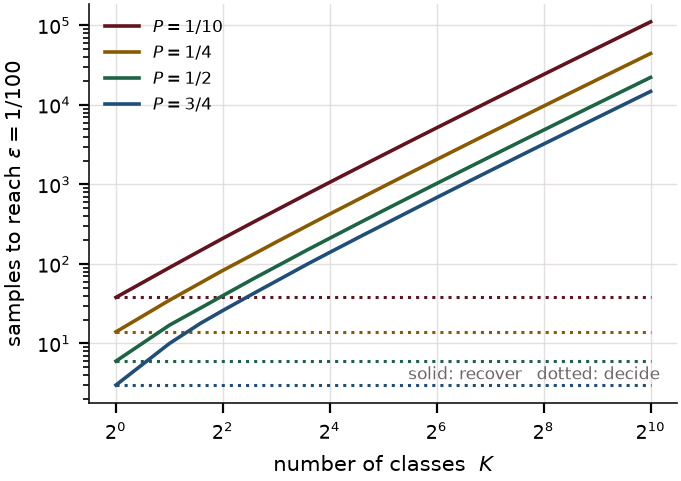
\includegraphics[width=\columnwidth]{support_fig4_counts.png}
\caption{Samples required to reach $\varepsilon=1/100$, for deciding (dotted) and for
recovering (solid), against the number of classes, at four values of $P$. Every point is an
exact integer obtained by inverting the closed forms \eqref{eq:sp-decide} and \eqref{eq:sp-recover},
not simulated: it is the least $N$ at which the exact risk falls below the tolerance. The
decide lines are horizontal because $K$ does not enter \eqref{eq:sp-decide}---that restates the
theorem rather than confirming it---while the recovery cost grows without bound beside them.
\NUM{}}
\label{fig:sp-counts}
\end{figure}

\begin{figure}[htbp]
\centering
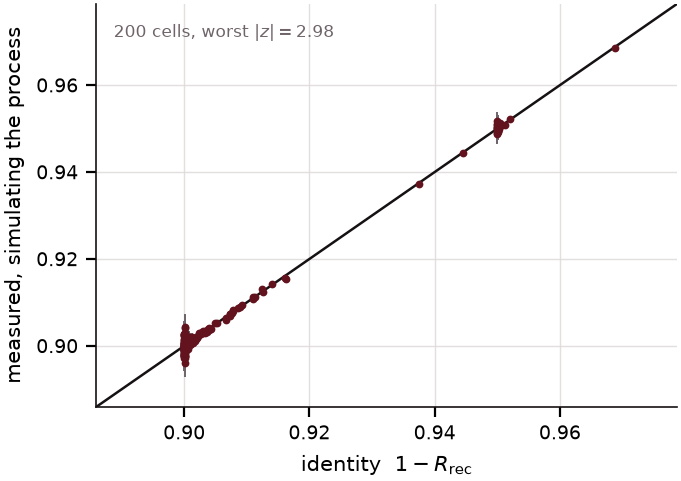
\includegraphics[width=\columnwidth]{support_fig6_identity.png}
\caption{The recovery identity against the process it is derived for. Each point is one cell
at its own recovery threshold: the horizontal coordinate is $1-R_{\mathrm{rec}}$ from
\eqref{eq:sp-recover}, the vertical is the frequency measured by simulating the sampling and the
coin flips, and the bars are two standard errors. The line is equality, not a fit. The
identity assumes nothing about how the classes interact, and the classes in the simulation do
interact---they compete for the same $N$ observations---so agreement here is a check on the
identity rather than on the arithmetic. \NUM{}}
\label{fig:sp-identity}
\end{figure}

\begin{figure}[htbp]
\centering
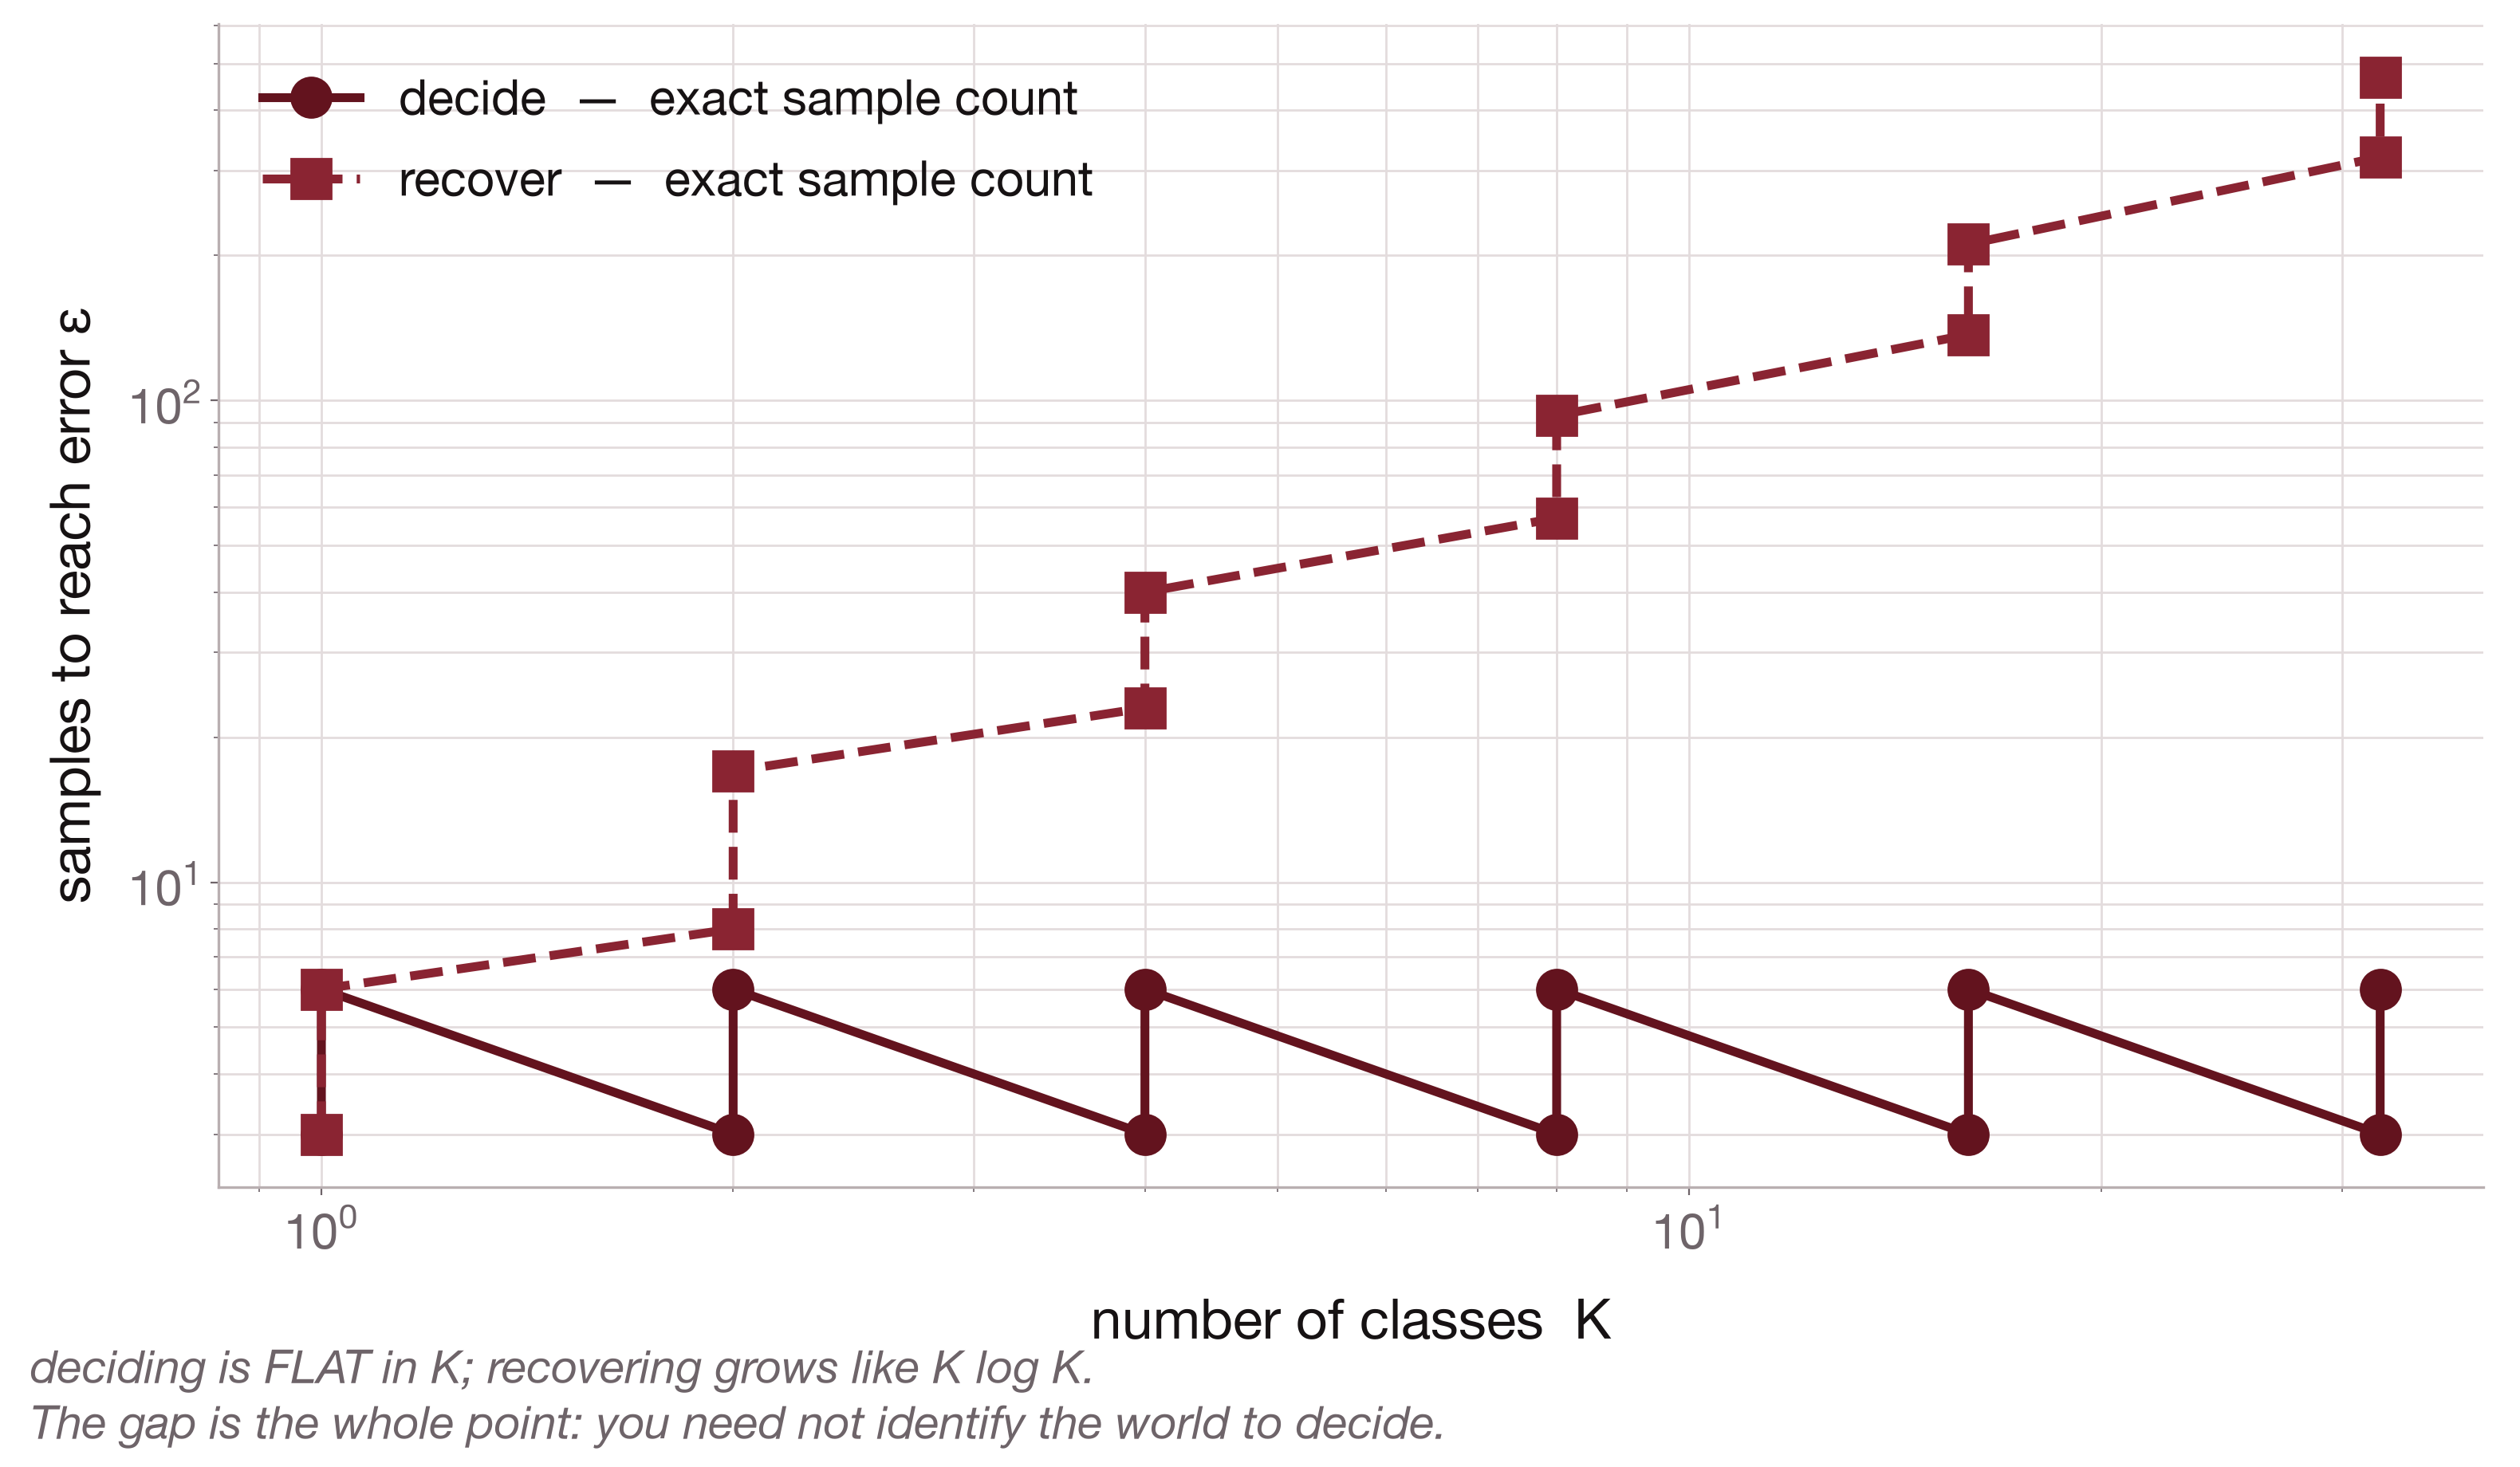
\includegraphics[width=\columnwidth]{support_fig1_separation.png}
\caption{Exact sample counts. Deciding is flat in the number of classes; recovering grows.
Both counts are exact integers computed from the closed forms rather than simulated, so the
widening gap is an identity against a growth rate.}
\label{fig:sp-separation}
\end{figure}

\subsection{The Comparison Is Between Two Thresholds}

Because both costs are defined as the least $N$ meeting the same $\varepsilon$, the ratio is a
quotient of integers and not a comparison against a rate with a hidden constant. It is also
not scale-free: at $\varepsilon=\tfrac{1}{10}$ and $K=2$ the ratio is $8/3\approx2.67$, at
$\varepsilon=\tfrac{1}{100}$ it is $17/6\approx2.83$. The ratio grows with $K$, which is the
claim, and moves slightly with $\varepsilon$, which is neither claimed nor surprising.

\subsection{The Decoder Is Optimal, Not Merely Flat}

With Theorem~\ref{thm:sp-minimax} the equivariant decoder is a least element of the achievable
worst-case risks, so no decision rule---randomised or not, adaptive or not---achieves a
smaller worst case on this problem. The quantifier is over all maps from observations to
actions, which in a finite setting is every rule there is.


\subsection{The Admissible Query Sets the Leakage Order}
\label{sec:qy-results}

\subsection{Reporting Protocol}

Both measurements are reported, with per-world rows, the equal-prior combination, the
bootstrap interval and the proved window. No run is excluded.

\subsection{The Measured Regret Lands Inside the Proved Window}

The order-$2$ measurement has per-sample $H^{2}=4.92\times10^{-4}$, requires $N=4{,}678$,
and shows equal-prior mean regret $0.008353$ with bootstrap interval
$[0.006888,0.009892]$ against the window $[0.001066,0.029298]$. The order-$1$ measurement
has $H^{2}=5.62\times10^{-5}$, requires $N=41{,}006$, and shows mean regret $0.009159$. Both
fall strictly inside their windows, and neither bootstrap interval crosses either end.

This is a consistency check on the chain rather than an independent confirmation of it---the
theorems are proved---but a chain with an arithmetic slip in any constant would fail it.

\begin{table}[htbp]
\caption{Two admissible measurements of one pair of worlds, $h=0.6$, $4000$ repetitions per
world. The worlds are identical across the two columns.}
\label{tab:qy-query}
\centering
\footnotesize
\begin{tabular}{@{}lrr@{}}
\toprule
Quantity & order $2$ & order $1$ \\
\midrule
Per-sample $H^{2}$      & $4.92\times10^{-4}$ & $5.62\times10^{-5}$ \\
Per-sample $L$          & $4.92\times10^{-4}$ & $5.62\times10^{-5}$ \\
Required $N$            & $4{,}678$           & $41{,}006$ \\
Measured regret         & $0.008353$          & $0.009159$ \\
Inside the window       & yes                 & yes \\
\bottomrule
\end{tabular}
\end{table}

\begin{table*}[t]
\caption{Full simulation record for the two admissible measurements of
Section~\ref{sec:qy-results}. The two worlds are identical across both measurements; only
$g$ differs. Regret is measured per world and then combined under an equal prior, and the
percentile bootstrap uses 2000 resamples. The proved window is
$[\frac{\gamma}{4}\rho^{2N},\,\frac{L_{\max}}{2}\rho^{N}]$ from Theorem~\ref{thm:qy-regret}
with $\gamma=13983/32768$ and $L_{\max}=2401/4096$, both exact rationals. Every measured value lies strictly
inside its window, and no bootstrap interval crosses either end.}
\label{tab:qy-fullquery}
\centering
\footnotesize
\setlength{\tabcolsep}{5pt}
\begin{tabular}{@{}llrrrrlr@{}}
\toprule
Measurement & World & $h$ & per-sample $H^{2}$ & $N$ & error rate & mean regret & s.e. \\
\midrule
\lean{g0\_normalised\_order2} & 0 & 0.6 & 4.922e-04 & 4,678 & 0.0150 & 0.008793 & 0.001127 \\
\lean{g0\_normalised\_order2} & 1 & 0.6 & 4.922e-04 & 4,678 & 0.0135 & 0.007913 & 0.001070 \\
\multicolumn{2}{@{}l}{\emph{equal prior}} & & & & & 0.008353 & \\
\multicolumn{2}{@{}l}{\emph{bootstrap CI95}} & & & & & [0.006888,\,0.009892] & \\
\multicolumn{2}{@{}l}{\emph{proved window}} & & & & & [0.001066,\,0.029298] & inside \\
\midrule
\lean{u\_normalised\_order1} & 0 & 0.6 & 5.615e-05 & 41,006 & 0.0155 & 0.009086 & 0.001145 \\
\lean{u\_normalised\_order1} & 1 & 0.6 & 5.615e-05 & 41,006 & 0.0158 & 0.009232 & 0.001154 \\
\multicolumn{2}{@{}l}{\emph{equal prior}} & & & & & 0.009159 & \\
\multicolumn{2}{@{}l}{\emph{bootstrap CI95}} & & & & & [0.007620,\,0.010844] & \\
\multicolumn{2}{@{}l}{\emph{proved window}} & & & & & [0.001067,\,0.029308] & inside \\
\bottomrule
\end{tabular}
\end{table*}


\begin{figure}[htbp]
\centering
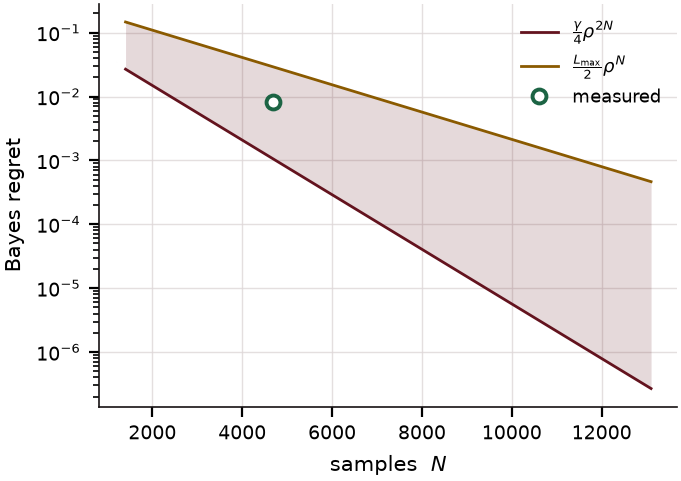
\includegraphics[width=\columnwidth]{query_fig5_window.png}
\caption{The proved regret window and the measurement inside it. The two envelopes are
\eqref{eq:qy-regret} evaluated with the exact constants $\gamma=13983/32768$ and
$L_{\max}=2401/4096$; they close at different rates in $N$---the lower like $\rho^{2N}$ and
the upper like $\rho^{N}$---so the window is wide on a logarithmic axis and narrows as the
sample count grows. The marker is the measured equal-prior regret of the order-$2$
measurement at its required $N$. A window this wide is a weak prediction and the figure is
drawn to make that visible rather than to hide it: what the measurement rules out is an
arithmetic slip in the constants, not a competing theory. \NUM{}}
\label{fig:qy-window}
\end{figure}

\subsection{The Same Worlds, a Different Legal Query, an Order of Magnitude}

The ratio $41{,}006/4{,}678\approx8.8$ is not a property of the worlds. They are identical
in both runs: same $f_{0}$, same $f_{1}$, same noise. The entire factor is attributable to
which measurement was admissible.

\begin{figure}[htbp]
\centering
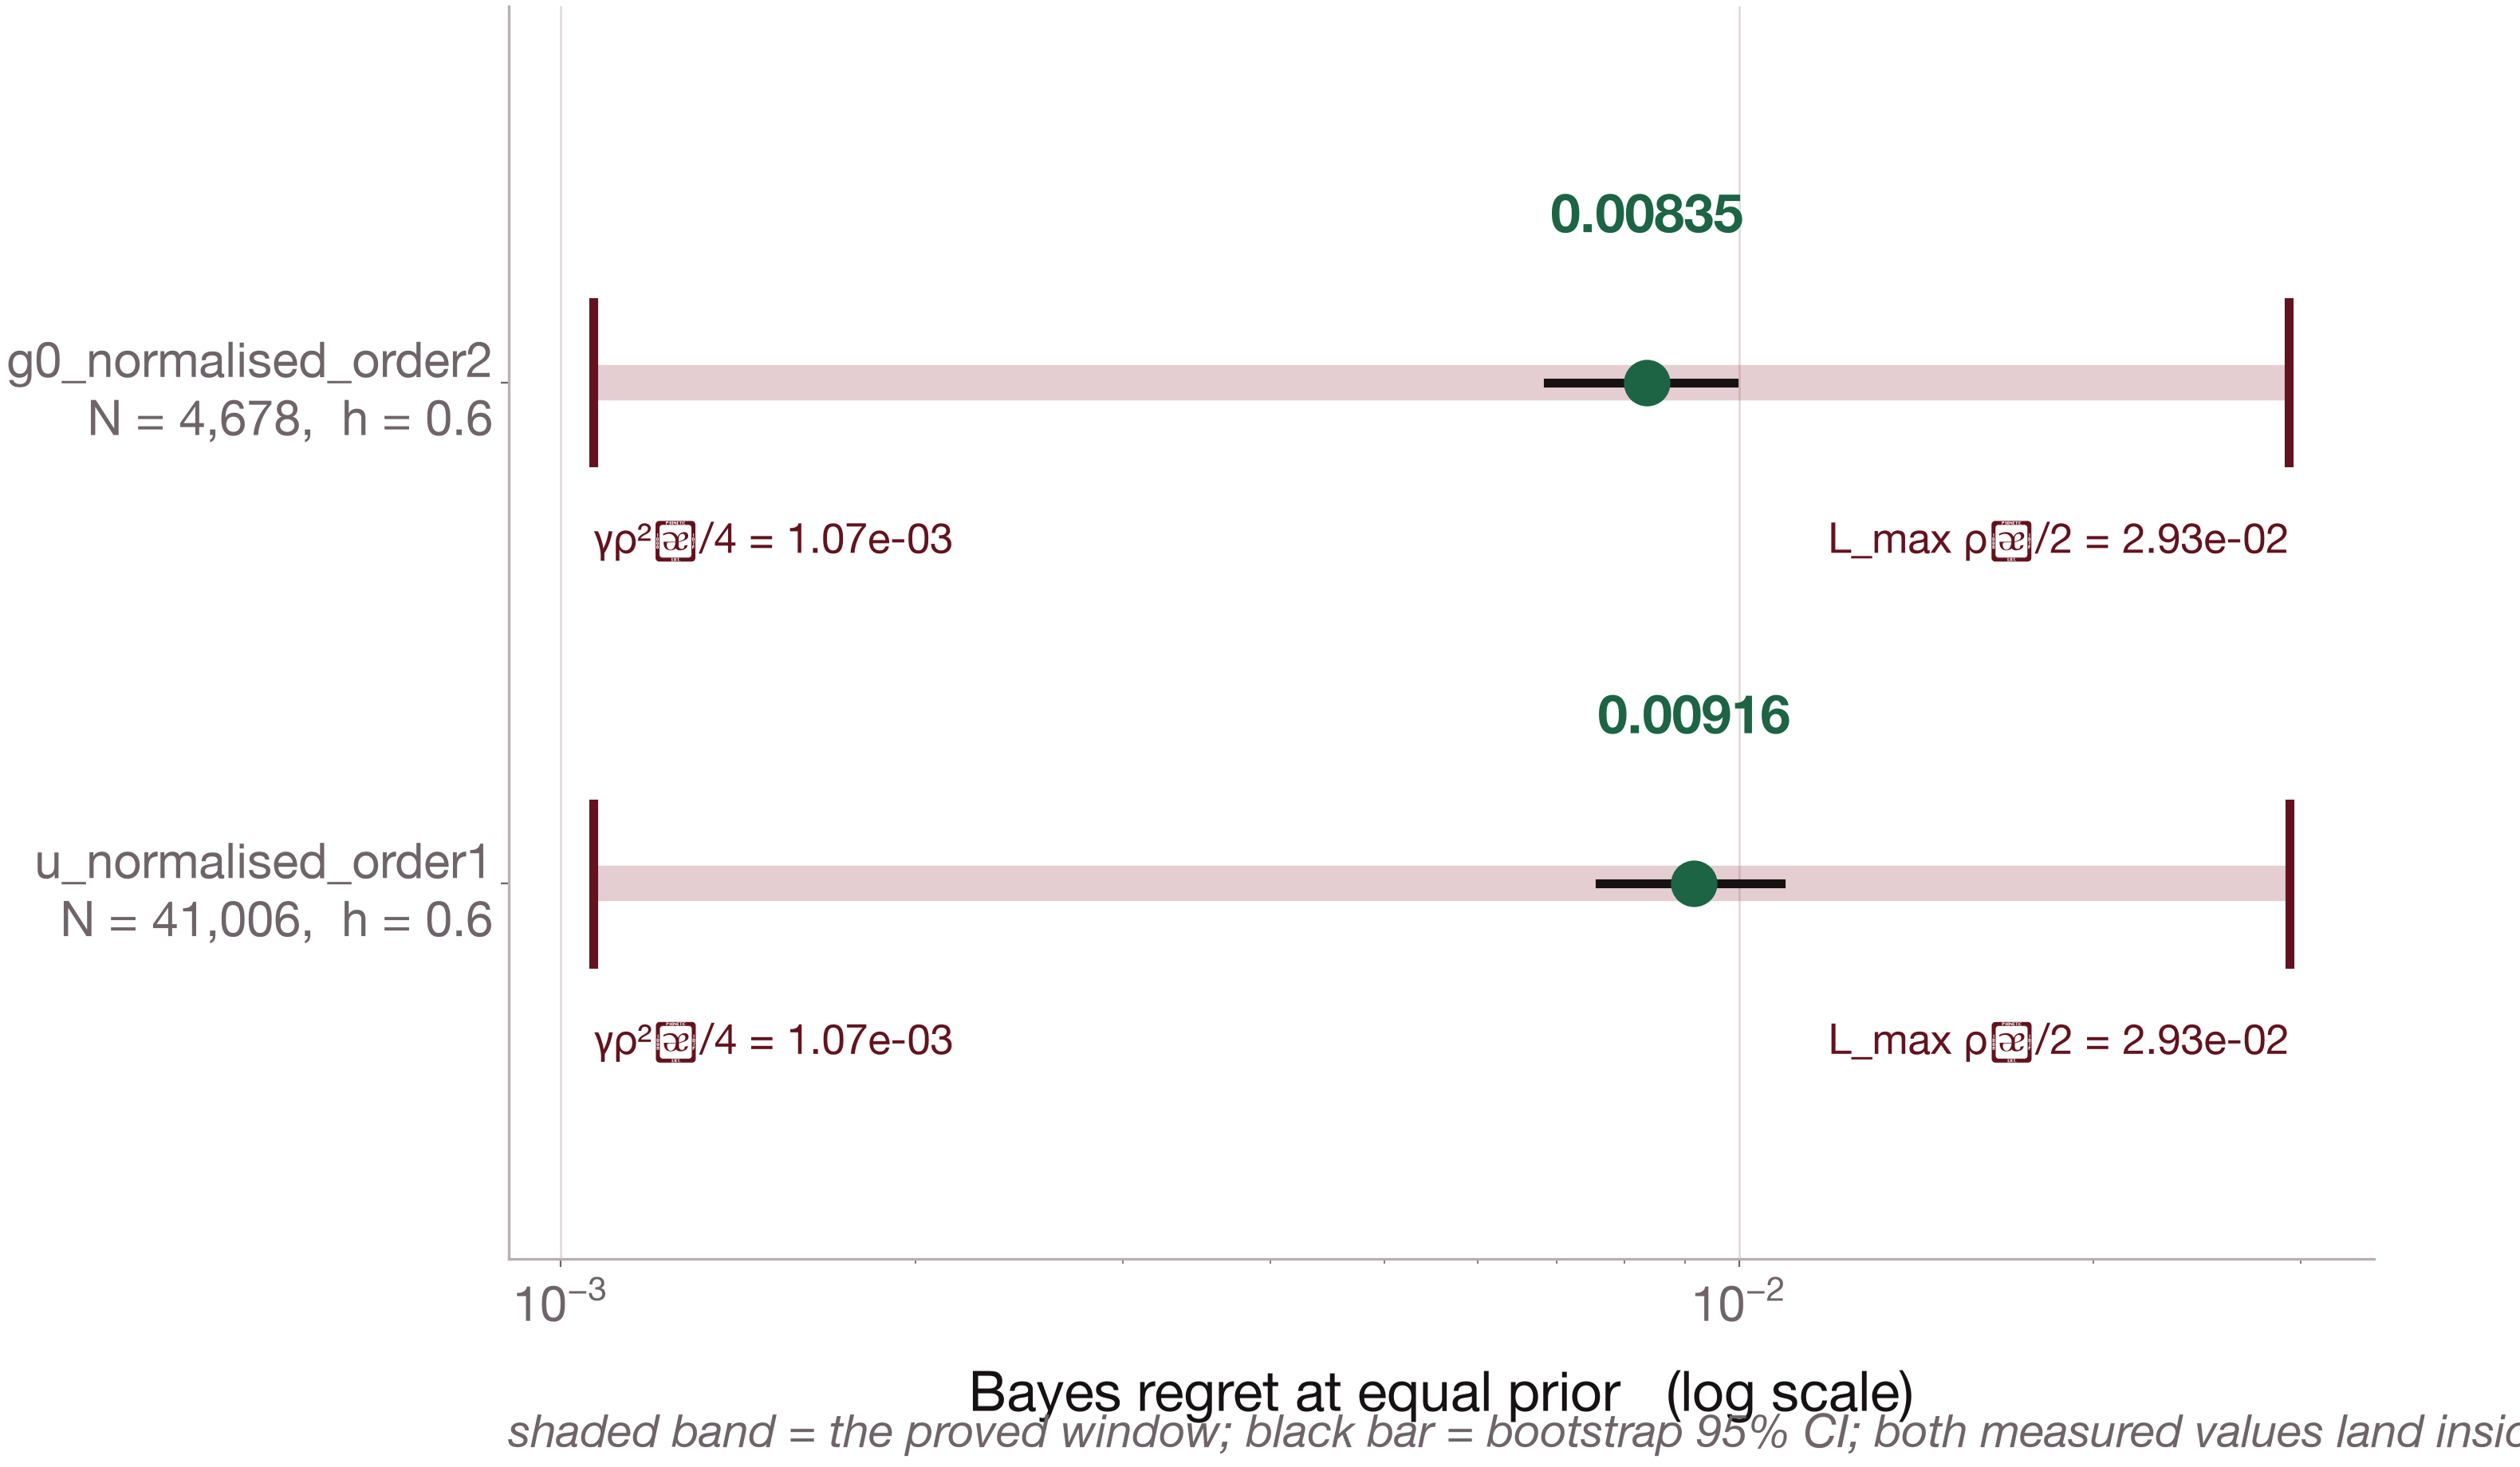
\includegraphics[width=\columnwidth]{query_fig1_regret.png}
\caption{Measured Bayes regret against the proved window of Theorem~\ref{thm:qy-regret} for two
admissible measurements of the same worlds. The shaded band is the window; the black bar is
a percentile bootstrap $95\%$ interval over $2000$ resamples.}
\label{fig:qy-regret}
\end{figure}

\subsection{Reading the Factor}

The factor is not a constant of the problem; it is $h^{-2(r_{1}-r_{2})}$ up to the explicit
constants of Theorem~\ref{thm:qy-sandwich}, with $r_{1}-r_{2}=1$ and $h=0.6$ here. Halving $h$
would roughly quadruple it. This is the operational content of ``the order is a property of
the query'': the penalty for the wrong measurement is not additive and does not wash out
with more data---it is an exponent, and it compounds as the regime gets harder.

\subsection{The Exponent Is $2r$ on Every Instance Drawn}
\label{sec:qy-e2results}

Experiment~E2 of Section~\ref{sec:qy-e2} draws two hundred instances and builds, on each, a
perturbation of designed leakage order $1$, $2$ and $3$. Three facts are reported in the order
in which they must be established.

First, the construction does what it claims. The self-check, which the run requires to pass
before it will report anything, finds the two worlds' level masses agreeing to
$1.1\times10^{-16}$---so they are identical at $h=0$ and the order is well posed---and the
independently recomputed order equal to the designed one on every check instance. Across the
sweep proper, the order recovered from the level coefficients equals the designed order in all
$600$ cells, with no cell falling into the tied-top-level case that Section~\ref{sec:qy-procedure}
sets aside. \NUM{}

Second, the exponent. Figure~\ref{fig:qy-order} plots $H^{2}$ against $h$ for the first three
instances drawn at each order---an arbitrary selection, not a chosen one, with the whole
population in Figure~\ref{fig:qy-slopes}; the three groups separate into fans of slope $2$, $4$ and $6$ and do
not cross. Fitted on the asymptotic tail, the slope deviates from $2r$ by $0.0052$ in
root-mean-square and by at most $0.0336$ over all $600$ cells, and the mean deviation is
$-0.0002$, $-0.0001$ and $-0.0020$ at the three orders---no bias at any of them. This is what
Theorem~\ref{thm:qy-sandwich} predicts, and the instances were drawn rather than chosen.
\NUM{}

Third, and least comfortable: the fit window is not a detail. Figure~\ref{fig:qy-slopes} shows the
same fits performed on the whole $h$ grid instead of its tail. They are biased low, and the
bias grows with the order---$-0.007$ at $r=1$, $-0.037$ at $r=2$, $-0.188$ at $r=3$, reaching
$-0.53$ on the worst cell. The reason is visible in Figure~\ref{fig:qy-order}: every curve bends
near $h\approx0.3$, where the next term of the expansion is not yet negligible, and a
higher-order curve spends more of the grid in that regime because its leading term is smaller.
An analyst who fits the whole range will conclude that a high-order query is better than it is,
by a margin that grows exactly where the effect being claimed is largest. The tail window is
declared in Section~\ref{sec:qy-e2} for that reason, and both fits are reported here rather than
only the favourable one.

One thing the experiment does \emph{not} show should be stated plainly, because a reader could
reasonably expect it. At the fixed scale $h=0.5$, the sample counts derived from
Theorem~\ref{thm:qy-samples} do not order by leakage order: the medians are $527$, $1{,}095$ and
$883$ at orders $1$, $2$ and $3$, so order $3$ sits below order $2$. There is no contradiction.
The order governs the \emph{rate} at which $H^{2}$ vanishes as $h\to0$, not its value at any
particular $h$, and at $h=0.5$ the constant in front still dominates. The instances behind the
three medians are independent draws rather than the same worlds measured three ways, so the
comparison is distributional and not paired; the paired statement is the one in
Table~\ref{tab:qy-query}, where the worlds are held fixed and only the measurement changes.
Where E2 does check the sample count against a realised error---$90$ cells simulated at the $N$
the theorem derives---all $90$ come in at or below the target, at mean error $0.016$ against a
target of $0.05$, so the derived count is conservative rather than tight. \NUM{}

\begin{figure}[htbp]
\centering
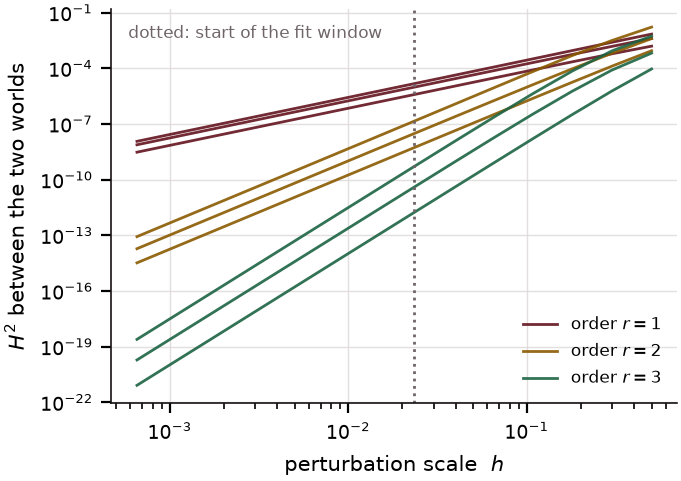
\includegraphics[width=\columnwidth]{query_fig3_order.png}
\caption{$H^{2}$ between two worlds sharing a level set, against the perturbation scale. Three
instances are drawn at each designed leakage order, and they are the first three the run
produced rather than three selected for the picture; the aggregate over all $600$ cells is
Figure~\ref{fig:qy-slopes}, and this figure is here to show the shape of a curve, not to carry
the claim. The three groups are fans of slope $2r$ and do not cross. Every curve bends near $h\approx0.3$, where the next term of the
expansion is still contributing; the dotted line marks where the fit window begins, chosen
before the fits were performed. Quadrature on the exact mixtures, verified stable to
$3\times10^{-13}$ against a grid twice as fine and twice as wide. \NUM{}}
\label{fig:qy-order}
\end{figure}

\begin{figure}[htbp]
\centering
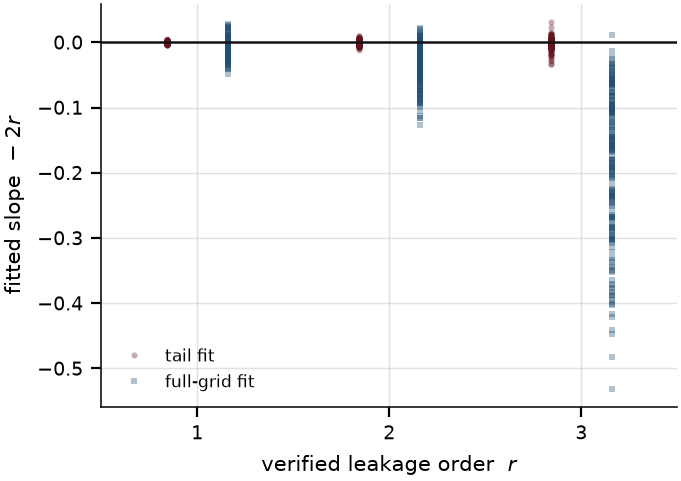
\includegraphics[width=\columnwidth]{query_fig6_slopes.png}
\caption{Fitted exponent minus the predicted $2r$, for all $600$ cells, under the two fit
windows. On the asymptotic tail (circles) the deviation is centred on zero at every order and
never exceeds $0.034$. On the full grid (squares) it is biased low, and the bias grows with the
order, because a higher-order curve spends more of the grid in the pre-asymptotic regime. The
figure is included to show what the choice of window costs, not to hide it. \NUM{}}
\label{fig:qy-slopes}
\end{figure}

\begin{figure}[htbp]
\centering
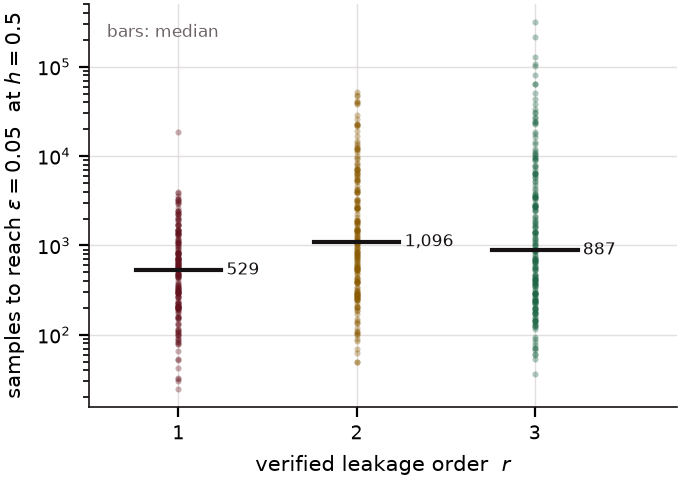
\includegraphics[width=\columnwidth]{query_fig4_samples.png}
\caption{Samples required to reach error $0.05$ at $h=0.5$, by verified leakage order; one
point per instance, bars at the medians. The distributions overlap heavily and their medians do
not increase with the order, which is the expected behaviour rather than an anomaly: the order
controls the rate at which $H^{2}$ vanishes as $h\to0$, and at a fixed moderate $h$ the leading
constant still dominates. Instances differ across the three columns, so this is a
distributional comparison and not a paired one. \NUM{}}
\label{fig:qy-samples}
\end{figure}

\subsection{The Exponent at Orders Four and Five}
\label{sec:qy-e3results}

Six hundred further cells, one hundred and twenty instances at each of five orders, with the
order verified from the level coefficients in every one. Orders one through three are
reproduced exactly as before---mean deviation $0.0000$, $-0.0000$ and $-0.0002$ from the
predicted $2r$. Order four is as clean: mean $-0.0003$, with every one of its
$120$ cells inside the reliability criterion. \NUM{}

Order five is where the measurement, not the law, gives out. The mean deviation is $-0.0136$
and the worst cell reaches $-0.21$. Figure~\ref{fig:qy-highorder} shows why that is a statement
about arithmetic: the flagged cells are almost all at order five, and they are flagged by a
criterion fixed before the run---a tail fit whose $R^{2}$ falls below $0.999$---rather than
by their disagreement with the prediction. At order five the usable window in $h$ is barely
one and a half decades wide, because $H^{2}$ must stay above the floor where double precision
still resolves it, and a slope fitted over that span with any curvature left in it is biased
low. Raising the floor from $10^{-22}$ to $10^{-18}$ between two runs of this experiment
moved order five's mean deviation from $-0.061$ to $-0.014$ and its reliable count from
$62$ of $120$ cells to $118$, which is the signature of a numerical limit rather than a
failing law.
\NUM{}

The honest summary is that the exponent $2r$ is confirmed on drawn instances for
$r\le4$, and that order five is consistent with it but measured at the edge of what
double-precision quadrature supports. Confirming order five properly needs extended-precision
quadrature, which is a different experiment and is not claimed here.

\begin{figure}[htbp]
\centering
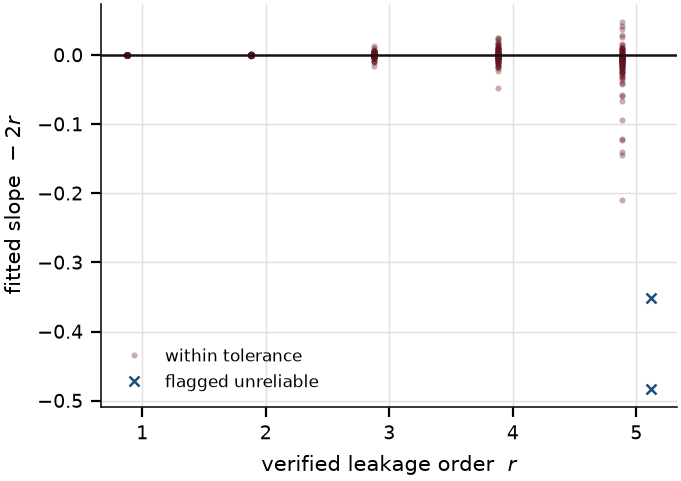
\includegraphics[width=\columnwidth]{query_fig7_highorder.png}
\caption{Fitted exponent minus the predicted $2r$ at five leakage orders, one hundred and
twenty instances each. Circles are cells whose tail fit meets the reliability criterion;
crosses are cells the criterion rejects, and they concentrate at order five, where the window
in $h$ left by double precision is narrowest. The rejection criterion is the quality of the
fit, fixed before the run, not the size of the disagreement---so the flagged cells were not
chosen for being inconvenient. \NUM{}}
\label{fig:qy-highorder}
\end{figure}

\subsection{How Near to Vanishing the Coefficient Gets}
\label{sec:qy-e4results}

Section~\ref{sec:qy-limits} calls the tied top level the most likely place for
Theorem~\ref{thm:qy-nonvanish} to fail in practice, and the proof shows why: the factorisation
that separates the terms needs the gap $v^{*}-v$ to be strictly positive, and at a tie the
argument returns $0=0$. What the proof cannot say is whether the \emph{conclusion} survives.
That has a measurable form. Experiment~E4 drives the top-level gap from $2\sigma$ down to
$10^{-3}\sigma$ by construction and measures $\|\Delta_{r}\|$ against the single largest term
it is assembled from. Two findings, and they point in opposite directions.

\emph{The hypothesis is essential.} The ratio falls, and it falls at slope $1.000$, $1.000$
and $1.000$ at orders one, two and three on a log-log axis---linearly in the gap, over three
decades, with no departure at either end. So the strict-largest hypothesis is not an artefact
of the proof technique that a cleverer argument could remove: the quantity the theorem is
about really does go to zero as the gap closes, and any statement covering the tied case would
have to say something different rather than something stronger.

\emph{Nothing pathological happens on the way.} Across all $2{,}160$ cells, not one had
$\Delta_{r}$ vanish. The approach to zero is smooth and it is exactly first order, which is
what the construction predicts and what Figure~\ref{fig:qy-tiedtop} shows: the two contributing
levels carry equal and opposite coefficients, so at separation $\delta$ they differ to first
order by $\delta$ times the derivative of a single term. There is no gap, no threshold and no
oscillation---the tie is a limit point, not a boundary. \NUM{}

For anyone attempting the tied case, that is the useful part. The difficulty is not that
$\Delta_{r}$ might vanish at some positive gap and has to be excluded; it is that the quantity
being bounded below degenerates continuously, so a bound covering the tie must carry the gap
explicitly rather than be uniform in it.

\begin{figure}[htbp]
\centering
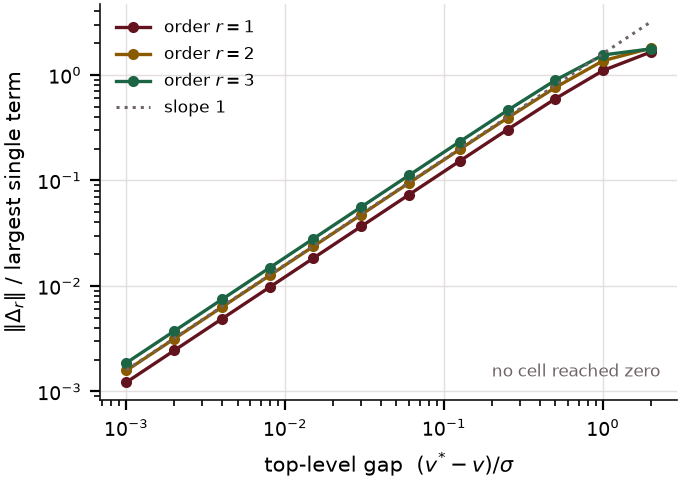
\includegraphics[width=\columnwidth]{query_fig9_tiedtop.png}
\caption{The assembled order-$r$ coefficient as the top-level gap closes, relative to the
largest single term it is built from. Medians over sixty instances per point, at three
orders, with the gap set by construction rather than by chance. All three fall at slope one
over three decades---linearly in the gap---so the strict-largest hypothesis of
Theorem~\ref{thm:qy-nonvanish} is essential, and the degeneration is smooth: no cell in the
sweep reached zero at any positive gap. \NUM{}}
\label{fig:qy-tiedtop}
\end{figure}


\section{Discussion}

\subsection{Deciding Without Identifying: An Exact Minimax Law}
\label{sec:sp-discussion}

\subsection{What the Results Establish}

The gap closed here is small to state and large in consequence. A constant-risk decoder is not
automatically a good one: constancy is a property of the decoder, optimality a property of the
problem, and without an infimum over rules the earlier statement was compatible with every
rule being bad, including this one.

The practical reading of the separation is that an experimenter facing many classes should not
pay for identification. The corollary for system design is that the question ``what do I need
to know?'' should be asked before ``how do I learn it?''. If the downstream decision is a
choice among actions rather than a report of the parameter, the identification cost may be
entirely avoidable, and Theorem~\ref{thm:sp-minimax} says the avoidance is not a heuristic.

\subsection{Shortcomings and Limitations}
\TODOPAR{Three things a reviewer will press, in order of severity. (i) The decoder is
not \emph{uniquely} optimal---any rule naming an unexplored tip attains the bound---so the
result constrains rather than selects, and the prose should say so where the optimality is
claimed. (ii) $R_{\mathrm{dec}}$'s independence of $K$ is an identity in the symmetric model
($a_{i}=b_{i}=1$, $p_{i}=P/K$, $P$ held fixed), not a discovered fact; Section~V-E says
``structural, not measured'' and that caveat belongs in the abstract. (iii) The decide side is
a closed form and the recovery side is an inclusion--exclusion identity inverted by bisection,
so the ``separation'' compares objects of different kinds. The coupon-collector fit
($c\in[0.916,0.966]$, $R^{2}\ge0.99996$) is strong evidence that an asymptotic closed form
exists; \emph{deriving it would close the comparison} and is probably a week's work.}

\emph{One prior, not a minimax theorem.} The prior is arbitrary but fixed: this is minimaxity
through one Bayes prior, and no saddle point is claimed. What is obtained is a value
lower-bounding the worst-case risk of every rule and achieved by one, which is the definition
of a minimax-optimal rule; what is not obtained is a least-favourable prior.

\emph{Everything is finite.} Attainment of the pointwise minimum is immediate in a finite
action set; with an infinite one the conclusion weakens to an infimum that may not be achieved.
The ease is in the proof rather than the statement---the earlier treatment had the same finite
setting and not the result---but the limitation is real for any extension.

\emph{The decoder is not uniquely optimal.} As Section~\ref{sec:sp-natural} shows, every rule
naming some unexplored tip attains the bound. The result constrains rather than selects.

\emph{Symmetry is doing work.} With an asymmetric prior the identification of the argmin with
the uniform decoder fails, so Theorem~\ref{thm:sp-minimax}'s conclusion about \emph{that} decoder
no longer follows.

\emph{The separation is model-specific.} Theorem~\ref{thm:sp-separation} holds on
$a_{i}=b_{i}=1$ with total unsafe mass fixed. It does not extend the fixed-$K$ constants,
which depend on $K$, and it says nothing about problems where the transcript is used for
something other than naming one safe tip.

\emph{The observation process is given.} Nothing here designs the sampling, which is exactly
what the decision-region literature does; the two are complementary rather than competing.

\subsection{Open Problems}

Whether the least-element conclusion survives an infinite action set, with attainment recovered
under a compactness hypothesis, is the first question. Whether the flatness of
\eqref{eq:sp-decide} in $K$ survives asymmetric classes---where the relabelling group is no longer
transitive and Proposition~\ref{prop:sp-symmetry} fails---is the second. Third, the separation
compares an exact decide cost against an inclusion--exclusion recovery threshold; a closed form
for the latter would make the comparison an identity on both sides. Finally, Theorem~\ref{thm:sp-threeworld} exhibits a
minimal unsafe triple but not a law: bounding the size of the smallest group of worlds
admitting no common safe decision, as a function of the support geometry, would connect this
analysis to the decision-region framework at the level of complexity rather than of
instances.


\subsection{The Admissible Query Sets the Leakage Order}
\label{sec:qy-discussion}

\subsection{What the Results Establish}

The result reframes what an experimenter controls. Where the parameter space is fixed by
nature, the measurement class is often a design choice, and the leakage order---hence the
exponent of the rate---moves with it. Theorem~\ref{thm:qy-nonvanish} is what licenses the
reframing: without it a vanishing order-$r$ coefficient would leave the order undefined and
the comparison between queries meaningless. Theorem~\ref{thm:qy-limit} then certifies that the
constant in front of the rate is real, so the comparison is between two genuine leading
terms.

\subsection{Shortcomings and Limitations}
\NOTEPAR{An earlier draft listed ``ties at the top'' as the most likely place for the
result to fail. That configuration does not exist: levels are distinct reals, and two that
coincide are one level carrying the sum of their coefficients. E4 (Fig.~\ref{fig:qy-tiedtop}) was
therefore measuring the approach to a \emph{vanishing} top coefficient---the exchanged levels
carry equal and opposite coefficients, so closing their separation drives the merged
coefficient to zero---which is a different and more useful thing to have measured.}
\label{sec:qy-limits}

\emph{A vanishing top coefficient is not formalised.} Theorem~\ref{thm:qy-nonvanish} asks that
the top level of the shared level set carry a non-zero coefficient. When it does not, the
mathematics is routine---restrict to the support of $c$ and apply the theorem at the largest
surviving level---but that step is not in Lean, so Algorithm~\ref{alg:qy-order} returns
\textsc{undetermined} there. This is a formalisation gap and not an open problem, and closing
it would remove the branch. An earlier version of this section described the uncovered case as
a tie between two top levels; that case does not arise, because levels are distinct reals and
two that coincide are one level carrying the sum of their coefficients.

What Section~\ref{sec:qy-e4results} measures is the approach to a vanishing top coefficient, not
to a tie. In the two-world construction the exchanged levels carry equal and opposite
coefficients, so driving their separation to zero drives the merged coefficient to zero as
well. The measurement is that the assembled coefficient degenerates \emph{linearly} in the
separation and never vanishes at a positive one: the hypothesis is therefore not removable,
and nothing discontinuous happens in the limit.

\emph{The window does not close.} The ends of \eqref{eq:qy-regret} separate as $N$ grows, so the
result localises regret without determining it. On the order-$2$ row the two ends differ by
roughly a factor of $27$, which reflects the $\rho^{2N}$ against $\rho^{N}$ gap rather than
any looseness in the measurement.

\emph{The paired comparison still uses two measurements, not a family.} Experiment~E2 supplies
the family for the \emph{rate}---six hundred cells at three orders, with the exponent fitted
rather than assumed---but its instances are independent draws, so it cannot pair. The factor
$8.8$ in Table~\ref{tab:qy-query} remains a single paired observation and should be read as one
instance of the prediction $h^{-2(r_{1}-r_{2})}$ rather than as a fitted exponent. What E2
adds, and what Section~\ref{sec:qy-e2results} reports, is that the sample counts do not order by
leakage order at a fixed $h$ at all: the paired factor is a statement about one pair of
measurements at one scale, and generalising it to ``higher order costs more samples'' is not
supported.

\emph{Small $h$ is reached only in the exact computation.} The asymptotic statements hold as
$h\downarrow0$, and at the simulated scale $h=0.6$ the remainder terms suppressed in
Theorem~\ref{thm:qy-sandwich} are not negligible---which is why the per-sample $H^{2}$ is computed
exactly there rather than from the envelope. Experiment~E2 does reach $h=6.5\times10^{-4}$, and
its curves show the remainder terms mattering out to about $h\approx0.3$; but it reaches that
regime by quadrature on the exact mixtures, not by sampling, and no simulated error rate is
reported below $h=0.5$. The asymptotic regime is therefore computed, never observed.

\emph{Nothing here is minimax.} Every result concerns a fixed pair and a fixed query, and
the dropped normalisation means the displayed expressions are not densities.

\subsection{Open Problems}

Closing the regret window---replacing \eqref{eq:qy-regret} by a two-sided bound whose ends agree
to a constant factor uniformly in $N$---is the first question, and it appears to need a
sharper handle on the likelihood-ratio test's error than the affinity supplies. The tied top
level is the second. Third, the map from a measurement to its leakage order is currently
computed case by case; a criterion reading $r$ off $g$ and the level structure directly would
turn the design question into a calculation. Finally, the limit in
Theorem~\ref{thm:qy-limit} is identified as an integral but not evaluated in closed form for any
non-trivial family.


\section{Conclusion}

\subsection{Deciding Without Identifying: An Exact Minimax Law}

The natural decoder---name a tip uniformly from the unexplored set---is not merely convenient.
Its risk is a function of the transcript alone, and it is a least element of the worst-case
risks achievable by \emph{any} decision rule. Deciding costs a number that does not grow with
the number of classes, while identifying the world does, so the two problems are separated
exactly rather than asymptotically. The general lesson is about what to prove rather than what
to build: the decoder was never in doubt as a practical choice, and what was in doubt was
whether implementing it was a compromise. Answering that took a quantifier over all rules
rather than a better decoder, and where a practical choice is obvious the useful theoretical
work is often to establish that it cannot be improved.



\subsection{The Admissible Query Sets the Leakage Order}

The leakage order is a property of the query, not of the parameter space, and the chain
establishing this is closed end to end: Gaussian derivatives built explicitly, the derivative
pushed through the finite sum, the order-$r$ coefficient proved not to vanish, $H^{2}$
sandwiched with explicit constants of matching exponent, converted into matching sample
counts, bracketed as regret, and shown to converge with a strictly positive limit. On an
instance where the worlds are held fixed, changing which measurement is legal changes the
sample requirement by a factor of $8.8$, and that factor is an exponent in $h$ rather than a
constant. For a practitioner the summary is a procedure rather than a theorem: enumerate the
levels of a candidate measurement, find the first order at which the coefficients fail to
cancel, check that the top level carrying weight there is strictly largest, and read the
sample requirement off $r$.



\section*{Acknowledgment}

\begin{thebibliography}{00}

\bibitem{javdani2014} S. Javdani, Y. Chen, A. Karbasi, A. Krause, J. A. Bagnell, and
S. Srinivasa, ``Near-optimal Bayesian active learning for decision making,'' in
\emph{Proc. 17th Int. Conf. Artificial Intelligence and Statistics (AISTATS)}, 2014.

\bibitem{golovin2011} D. Golovin and A. Krause, ``Adaptive submodularity: Theory and
applications in active learning and stochastic optimization,'' \emph{J. Artif. Intell. Res.},
vol.~42, pp.~427--486, 2011.

\bibitem{lehmann1998} E. L. Lehmann and G. Casella, \emph{Theory of Point Estimation},
2nd ed. New York, NY: Springer, 1998.

\bibitem{wald1950} A. Wald, \emph{Statistical Decision Functions}. New York, NY: Wiley, 1950.

\bibitem{motwani1995} R. Motwani and P. Raghavan, \emph{Randomized Algorithms}. Cambridge,
U.K.: Cambridge Univ. Press, 1995.

\bibitem{bennouna2026} A. Bennouna, O. Bennouna, S. Amin, and A. Ozdaglar, ``Data
informativeness in linear optimization under uncertainty,'' 2026.

\bibitem{mathlib2020} The mathlib Community, ``The Lean mathematical library,'' in
\emph{Proc. 9th ACM SIGPLAN Int. Conf. Certified Programs and Proofs (CPP)}, 2020,
pp.~367--381.

\bibitem{demoura2021} L. de Moura and S. Ullrich, ``The Lean 4 theorem prover and
programming language,'' in \emph{Proc. 28th Int. Conf. Automated Deduction (CADE)}, 2021,
pp.~625--635.

\bibitem{lecam1973} L. Le Cam, ``Convergence of estimates under dimensionality
restrictions,'' \emph{Ann. Statist.}, vol.~1, pp.~38--53, 1973.

\bibitem{ibragimov1981} I. A. Ibragimov and R. Z. Has'minskii, \emph{Statistical Estimation:
Asymptotic Theory}. New York, NY: Springer, 1981.

\bibitem{tsybakov2009} A. B. Tsybakov, \emph{Introduction to Nonparametric Estimation}.
New York, NY: Springer, 2009.

\bibitem{ho2015} N. Ho and X. Nguyen, ``Identifiability and optimal rates of convergence
for parameters of multiple types in finite mixtures,'' arXiv:1501.02497, 2015.

\bibitem{dwivedi2019} R. Dwivedi, N. Ho, K. Khamaru, M. J. Wainwright, M. I. Jordan, and
B. Yu, ``Sharp analysis of expectation-maximization for weakly identifiable models,'' in
\emph{Proc. 23rd Int. Conf. Artificial Intelligence and Statistics (AISTATS)}, 2020.

\bibitem{wei2020} Y. Wei and X. Nguyen, ``Convergence of de Finetti's mixing measure in
latent structure models for observed exchangeable sequences,'' arXiv:2004.05542, 2020.

\bibitem{chen1995} J. Chen, ``Optimal rate of convergence for finite mixture models,''
\emph{Ann. Statist.}, vol.~23, no.~1, pp.~221--233, 1995.

\bibitem{heinrich2018} P. Heinrich and J. Kahn, ``Strong identifiability and optimal minimax
rates for finite mixture estimation,'' \emph{Ann. Statist.}, vol.~46, no.~6A,
pp.~2844--2870, 2018.

\bibitem{szego1939} G. Szeg\H{o}, \emph{Orthogonal Polynomials}. Providence, RI: American
Mathematical Society, 1939.

\end{thebibliography}

\appendices
\section{Complete statement inventory}
\label{app:sp-inventory}

The Support strand contributes $183$ axiom-audited theorems and lemmas across its accepted modules. Those that any step of this paper uses are displayed in Section~\ref{sec:sp-setting}, beside the step that consumes them. This appendix reproduces the \emph{complete} chain---every audited statement of the strand, grouped by module, including the ones already shown---so that the development can be read end to end without reassembling it from the body.

Each entry is a symbol-level transliteration of the Lean statement: Unicode maps to the corresponding \LaTeX{} symbol and identifiers are set upright, but no structure is rewritten and no hypothesis is dropped. Binders are listed as the prover has them and the turnstile $\vdash$ separates them from the conclusion. Every entry carries an acceptance receipt and an axiom audit confining it to $\{\textsf{propext},\textsf{Classical.choice},\textsf{Quot.sound}\}$; none contains \texttt{sorry}.

\vspace{4pt}\noindent\rule{\columnwidth}{0.4pt}\par\vspace{2pt}
\noindent\textbf{Module \lean{LeanSupportBayesMinimaxV1}}\par\vspace{3pt}

\noindent\textbf{A\,1}\quad\lean{adm\_eq\_empty\_of\_lt}
{\footnotesize\[ (\mathit{b} : \mathbb{N} ),\; (\mathit{S} : \mathit{Finset} (\mathit{Fin} \mathit{m})),\; (\mathit{hlt} : \mathit{b} < \mathit{S}.\mathit{card}) \;\vdash\; \mathit{adm} \mathit{b} \mathit{S} = \emptyset \]}

\noindent\textbf{A\,2}\quad\lean{bayes\_minimax}
{\footnotesize\[ \begin{aligned}[t]
&(\mathit{b} : \mathbb{N} ),\; (\mathit{p} : \mathbb{R} ),\; (\mathit{hp} : 0 \leq \mathit{p}),\; (\mathit{hbp} : (\mathit{b} : \mathbb{R} ) * \mathit{p} \leq 1),\\
&\quad \; (\mathit{hbm} : \mathit{b} < \mathit{m}),\; (\mathit{j0} : \mathit{Fin} \mathit{m})\\
\vdash\;&\mathit{IsLeast} \{ \mathit{r} : \mathbb{R} | \exists \mathit{D} : \mathit{Decoder} \mathit{m} \mathit{N}, \mathit{r} = \mathit{risk} \mathit{b} \mathit{p} \mathit{D}\} (\mathit{bayesValue} \mathit{m} \mathit{b} \mathit{N} \mathit{p})
\end{aligned} \]}

\noindent\textbf{A\,3}\quad\lean{count\_add}
{\footnotesize\[ (\mathit{h} : \mathit{Transcript} \mathit{m} \mathit{N}) \;\vdash\; \mathit{emptyCount} \mathit{h} + \mathit{tipCount} \mathit{h} = \mathit{N} \]}

\noindent\textbf{A\,4}\quad\lean{floorAt\_eq\_sFrac}
{\footnotesize\[ \begin{aligned}[t]
&(\mathit{m} \mathit{b} : \mathbb{N} ),\; (\mathit{hbm} : \mathit{b} \leq \mathit{m}),\; (\mathit{h} : \mathit{Transcript} \mathit{m} \mathit{N})\\
\vdash\;&\mathit{floorAt} \mathit{m} \mathit{b} \mathit{h} = \mathit{sFrac} \mathit{m} \mathit{b} \mathit{h}
\end{aligned} \]}

\noindent\textbf{A\,5}\quad\lean{image\_transport}
{\footnotesize\[ \begin{aligned}[t]
&(\mathit{W} \mathit{W'} : \mathit{Finset} (\mathit{Fin} \mathit{m})),\; (\mathit{hc} : \mathit{W}.\mathit{card} = \mathit{W'}.\mathit{card})\\
\vdash\;&\mathit{W}.\mathit{image} (\mathit{transport} \mathit{W} \mathit{W'} \mathit{hc}) = \mathit{W'}
\end{aligned} \]}

\noindent\textbf{A\,6}\quad\lean{joint\_eq\_mass\_of\_seen}
{\footnotesize\[ \begin{aligned}[t]
&(\mathit{b} : \mathbb{N} ),\; (\mathit{p} : \mathbb{R} ),\; (\mathit{h} : \mathit{Transcript} \mathit{m} \mathit{N}),\; (\mathit{j} : \mathit{Fin} \mathit{m}),\\
&\quad \; (\mathit{hj} : \mathit{j} \in \mathit{seen} \mathit{h})\\
\vdash\;&\mathit{joint} \mathit{b} \mathit{p} \mathit{h} \mathit{j} = \mathit{mass} \mathit{b} \mathit{p} \mathit{h}
\end{aligned} \]}

\noindent\textbf{A\,7}\quad\lean{joint\_ge}
{\footnotesize\[ \begin{aligned}[t]
&(\mathit{b} : \mathbb{N} ),\; (\mathit{p} : \mathbb{R} ),\; (\mathit{hp} : 0 \leq \mathit{p}),\; (\mathit{hbp} : (\mathit{b} : \mathbb{R} ) * \mathit{p} \leq 1),\\
&\quad \; (\mathit{hbm} : \mathit{b} \leq \mathit{m}),\; (\mathit{h} : \mathit{Transcript} \mathit{m} \mathit{N}),\; (\mathit{j} : \mathit{Fin} \mathit{m})\\
\vdash\;&\mathit{mass} \mathit{b} \mathit{p} \mathit{h} * \mathit{sFrac} \mathit{m} \mathit{b} \mathit{h} \leq \mathit{joint} \mathit{b} \mathit{p} \mathit{h} \mathit{j}
\end{aligned} \]}

\noindent\textbf{A\,8}\quad\lean{joint\_mul\_unseen}
{\footnotesize\[ \begin{aligned}[t]
&(\mathit{b} : \mathbb{N} ),\; (\mathit{p} : \mathbb{R} ),\; (\mathit{h} : \mathit{Transcript} \mathit{m} \mathit{N}),\; (\mathit{j} : \mathit{Fin} \mathit{m}),\\
&\quad \; (\mathit{hj} : \mathit{j} \notin \mathit{seen} \mathit{h})\\
\vdash\;&\mathit{joint} \mathit{b} \mathit{p} \mathit{h} \mathit{j} * ((\mathit{m} - (\mathit{seen} \mathit{h}).\mathit{card} : \mathbb{N} ) : \mathbb{R} ) =\\
&\quad \mathit{mass} \mathit{b} \mathit{p} \mathit{h} * ((\mathit{b} - (\mathit{seen} \mathit{h}).\mathit{card} : \mathbb{N} ) : \mathbb{R} )
\end{aligned} \]}

\noindent\textbf{A\,9}\quad\lean{lik\_eq}
{\footnotesize\[ \begin{aligned}[t]
&(\mathit{b} : \mathbb{N} ),\; (\mathit{p} : \mathbb{R} ),\; (\mathit{W} : \mathit{Finset} (\mathit{Fin} \mathit{m})),\; (\mathit{h} : \mathit{Transcript} \mathit{m} \mathit{N})\\
\vdash\;&\mathit{lik} \mathit{b} \mathit{p} \mathit{W} \mathit{h} = \mathbf{if} \mathit{seen} \mathit{h} \subseteq \mathit{W} \mathbf{then} \mathit{likC} \mathit{b} \mathit{p} \mathit{h} \mathbf{else} 0
\end{aligned} \]}

\noindent\textbf{A\,10}\quad\lean{lik\_nonneg}
{\footnotesize\[ \begin{aligned}[t]
&(\mathit{b} : \mathbb{N} ),\; (\mathit{p} : \mathbb{R} ),\; (\mathit{hp} : 0 \leq \mathit{p}),\; (\mathit{hbp} : (\mathit{b} : \mathbb{R} ) * \mathit{p} \leq 1),\\
&\quad \; (\mathit{W} : \mathit{Finset} (\mathit{Fin} \mathit{m})),\; (\mathit{h} : \mathit{Transcript} \mathit{m} \mathit{N})\\
\vdash\;&0 \leq \mathit{lik} \mathit{b} \mathit{p} \mathit{W} \mathit{h}
\end{aligned} \]}

\noindent\textbf{A\,11}\quad\lean{lik\_relabel}
{\footnotesize\[ \begin{aligned}[t]
&(\mathit{b} : \mathbb{N} ),\; (\mathit{p} : \mathbb{R} ),\; (\sigma : \mathit{Equiv}.\mathit{Perm} (\mathit{Fin} \mathit{m})),\; (\mathit{W} : \mathit{Finset} (\mathit{Fin} \mathit{m}))\\
&\quad ,\; (\mathit{h} : \mathit{Transcript} \mathit{m} \mathit{N})\\
\vdash\;&\mathit{lik} \mathit{b} \mathit{p} (\mathit{W}.\mathit{image} \sigma ) (\mathit{relabel} \sigma \mathit{h}) = \mathit{lik} \mathit{b} \mathit{p} \mathit{W} \mathit{h}
\end{aligned} \]}

\noindent\textbf{A\,12}\quad\lean{mass\_eq\_zero\_of\_lt}
{\footnotesize\[ \begin{aligned}[t]
&(\mathit{b} : \mathbb{N} ),\; (\mathit{p} : \mathbb{R} ),\; (\mathit{h} : \mathit{Transcript} \mathit{m} \mathit{N}),\; (\mathit{hlt} : \mathit{b} < (\mathit{seen} \mathit{h}).\\
&\quad \mathit{card})\\
\vdash\;&\mathit{mass} \mathit{b} \mathit{p} \mathit{h} = 0
\end{aligned} \]}

\noindent\textbf{A\,13}\quad\lean{mem\_seen}
{\footnotesize\[ \begin{aligned}[t]
&\{ \mathit{h} : \mathit{Transcript} \mathit{m} \mathit{N}\},\; \{ \mathit{j} : \mathit{Fin} \mathit{m}\}\\
\vdash\;&\mathit{j} \in \mathit{seen} \mathit{h} \leftrightarrow \exists \mathit{i}, \mathit{h} \mathit{i} = \mathit{some} \mathit{j}
\end{aligned} \]}

\noindent\textbf{A\,14}\quad\lean{passive\_minimax}
{\footnotesize\[ \begin{aligned}[t]
&(\mathit{b} : \mathbb{N} ),\; (\mathit{p} : \mathbb{R} ),\; (\mathit{hp} : 0 \leq \mathit{p}),\; (\mathit{hbp} : (\mathit{b} : \mathbb{R} ) * \mathit{p} \leq 1),\\
&\quad \; (\mathit{hbm} : \mathit{b} < \mathit{m}),\; (\mathit{j0} : \mathit{Fin} \mathit{m}),\; (\mathit{hne} : (\mathit{worlds} \mathit{m} \mathit{b}).\mathit{Nonempty})\\
\vdash\;&\mathit{IsLeast} \{ \mathit{r} : \mathbb{R} | \exists \mathit{D} : \mathit{Decoder} \mathit{m} \mathit{N}, \mathit{r} = (\mathit{worlds} \mathit{m} \mathit{b}).\mathit{sup'} \mathit{hne} (\mathbf{fun} \mathit{W}\\
&\quad => \mathit{worldRisk} \mathit{b} \mathit{p} \mathit{W} \mathit{D})\} (\mathit{bayesValue} \mathit{m} \mathit{b} \mathit{N} \mathit{p})
\end{aligned} \]}

\noindent\textbf{A\,15}\quad\lean{risk\_ge}
{\footnotesize\[ \begin{aligned}[t]
&(\mathit{b} : \mathbb{N} ),\; (\mathit{p} : \mathbb{R} ),\; (\mathit{hp} : 0 \leq \mathit{p}),\; (\mathit{hbp} : (\mathit{b} : \mathbb{R} ) * \mathit{p} \leq 1),\\
&\quad \; (\mathit{hbm} : \mathit{b} \leq \mathit{m}),\; (\mathit{D} : \mathit{Decoder} \mathit{m} \mathit{N})\\
\vdash\;&\mathit{bayesValue} \mathit{m} \mathit{b} \mathit{N} \mathit{p} \leq \mathit{risk} \mathit{b} \mathit{p} \mathit{D}
\end{aligned} \]}

\noindent\textbf{A\,16}\quad\lean{risk\_mul\_choose}
{\footnotesize\[ \begin{aligned}[t]
&(\mathit{b} : \mathbb{N} ),\; (\mathit{p} : \mathbb{R} ),\; (\mathit{hbm} : \mathit{b} \leq \mathit{m}),\; (\mathit{D} : \mathit{Decoder} \mathit{m} \mathit{N})\\
\vdash\;&\mathit{risk} \mathit{b} \mathit{p} \mathit{D} * (\mathit{m}.\mathit{choose} \mathit{b} : \mathbb{R} ) = \textstyle\sum \mathit{W} \in \mathit{worlds} \mathit{m} \mathit{b},\\
&\quad \mathit{worldRisk} \mathit{b} \mathit{p} \mathit{W} \mathit{D}
\end{aligned} \]}

\noindent\textbf{A\,17}\quad\lean{risk\_uniformUnseen}
{\footnotesize\[ \begin{aligned}[t]
&(\mathit{b} : \mathbb{N} ),\; (\mathit{p} : \mathbb{R} ),\; (\mathit{hp} : 0 \leq \mathit{p}),\; (\mathit{hbp} : (\mathit{b} : \mathbb{R} ) * \mathit{p} \leq 1),\\
&\quad \; (\mathit{hbm} : \mathit{b} < \mathit{m}),\; (\mathit{j0} : \mathit{Fin} \mathit{m})\\
\vdash\;&\mathit{risk} \mathit{b} \mathit{p} (\mathit{uniformUnseen} \mathit{N} \mathit{j0}) = \mathit{bayesValue} \mathit{m} \mathit{b} \mathit{N} \mathit{p}
\end{aligned} \]}

\noindent\textbf{A\,18}\quad\lean{seen\_relabel}
{\footnotesize\[ \begin{aligned}[t]
&(\sigma : \mathit{Equiv}.\mathit{Perm} (\mathit{Fin} \mathit{m})),\; (\mathit{h} : \mathit{Transcript} \mathit{m} \mathit{N})\\
\vdash\;&\mathit{seen} (\mathit{relabel} \sigma \mathit{h}) = (\mathit{seen} \mathit{h}).\mathit{image} \sigma
\end{aligned} \]}

\noindent\textbf{A\,19}\quad\lean{sum\_draw}
{\footnotesize\[ \begin{aligned}[t]
&(\mathit{b} : \mathbb{N} ),\; (\mathit{p} : \mathbb{R} ),\; (\mathit{W} : \mathit{Finset} (\mathit{Fin} \mathit{m})),\; (\mathit{hW} : \mathit{W}.\mathit{card} = \mathit{b})\\
\vdash\;&\textstyle\sum \mathit{o} : \mathit{Obs} \mathit{m}, \mathit{draw} \mathit{b} \mathit{p} \mathit{W} \mathit{o} = 1
\end{aligned} \]}

\noindent\textbf{A\,20}\quad\lean{sum\_lik}
{\footnotesize\[ \begin{aligned}[t]
&(\mathit{b} : \mathbb{N} ),\; (\mathit{p} : \mathbb{R} ),\; (\mathit{h} : \mathit{Transcript} \mathit{m} \mathit{N})\\
\vdash\;&\textstyle\sum \mathit{W} \in \mathit{worlds} \mathit{m} \mathit{b}, \mathit{lik} \mathit{b} \mathit{p} \mathit{W} \mathit{h} = \mathit{likC} \mathit{b} \mathit{p} \mathit{h} * ((\mathit{adm} \mathit{b} (\mathit{seen} \mathit{h})).\mathit{card} :\\
&\quad \mathbb{R} )
\end{aligned} \]}

\noindent\textbf{A\,21}\quad\lean{sum\_lik\_mem}
{\footnotesize\[ \begin{aligned}[t]
&(\mathit{b} : \mathbb{N} ),\; (\mathit{p} : \mathbb{R} ),\; (\mathit{h} : \mathit{Transcript} \mathit{m} \mathit{N}),\; (\mathit{j} : \mathit{Fin} \mathit{m})\\
\vdash\;&\textstyle\sum \mathit{W} \in \mathit{worlds} \mathit{m} \mathit{b}, (\mathbf{if} \mathit{j} \in \mathit{W} \mathbf{then} \mathit{lik} \mathit{b} \mathit{p} \mathit{W} \mathit{h} \mathbf{else} 0) =\\
&\quad \mathit{likC} \mathit{b} \mathit{p} \mathit{h} * ((\mathit{admWith} \mathit{b} (\mathit{seen} \mathit{h}) \mathit{j}).\mathit{card} : \mathbb{R} )
\end{aligned} \]}

\noindent\textbf{A\,22}\quad\lean{sum\_lik\_transcripts}
{\footnotesize\[ \begin{aligned}[t]
&(\mathit{b} : \mathbb{N} ),\; (\mathit{p} : \mathbb{R} ),\; (\mathit{W} : \mathit{Finset} (\mathit{Fin} \mathit{m})),\; (\mathit{hW} : \mathit{W}.\mathit{card} = \mathit{b})\\
\vdash\;&\textstyle\sum \mathit{h} : \mathit{Transcript} \mathit{m} \mathit{N}, \mathit{lik} \mathit{b} \mathit{p} \mathit{W} \mathit{h} = 1
\end{aligned} \]}

\noindent\textbf{A\,23}\quad\lean{sum\_mass\_eq\_one}
{\footnotesize\[ \begin{aligned}[t]
&(\mathit{b} : \mathbb{N} ),\; (\mathit{p} : \mathbb{R} ),\; (\mathit{hbm} : \mathit{b} \leq \mathit{m})\\
\vdash\;&\textstyle\sum \mathit{h} : \mathit{Transcript} \mathit{m} \mathit{N}, \mathit{mass} \mathit{b} \mathit{p} \mathit{h} = 1
\end{aligned} \]}

\noindent\textbf{A\,24}\quad\lean{transport\_mem}
{\footnotesize\[ \begin{aligned}[t]
&(\mathit{W} \mathit{W'} : \mathit{Finset} (\mathit{Fin} \mathit{m})),\; (\mathit{hc} : \mathit{W}.\mathit{card} = \mathit{W'}.\mathit{card}),\; (\mathit{x} : \mathit{Fin} \mathit{m})\\
\vdash\;&(\mathit{x} \in \mathit{W} \leftrightarrow \mathit{transport} \mathit{W} \mathit{W'} \mathit{hc} \mathit{x} \in \mathit{W'})
\end{aligned} \]}

\noindent\textbf{A\,25}\quad\lean{uuAlpha\_relabel}
{\footnotesize\[ \begin{aligned}[t]
&(\mathit{j0} : \mathit{Fin} \mathit{m}),\; (\sigma : \mathit{Equiv}.\mathit{Perm} (\mathit{Fin} \mathit{m})),\; (\mathit{h} : \mathit{Transcript} \mathit{m} \mathit{N}),\\
&\quad \; (\mathit{hne} : \mathit{seen} \mathit{h} \neq \mathit{univ}),\; (\mathit{j} : \mathit{Fin} \mathit{m})\\
\vdash\;&\mathit{uuAlpha} \mathit{j0} (\mathit{relabel} \sigma \mathit{h}) (\sigma \mathit{j}) = \mathit{uuAlpha} \mathit{j0} \mathit{h} \mathit{j}
\end{aligned} \]}

\noindent\textbf{A\,26}\quad\lean{uuAlpha\_sums}
{\footnotesize\[ (\mathit{j0} : \mathit{Fin} \mathit{m}),\; (\mathit{h} : \mathit{Transcript} \mathit{m} \mathit{N}) \;\vdash\; \textstyle\sum \mathit{j}, \mathit{uuAlpha} \mathit{j0} \mathit{h} \mathit{j} = 1 \]}

\noindent\textbf{A\,27}\quad\lean{worldRisk\_uu\_const}
{\footnotesize\[ \begin{aligned}[t]
&(\mathit{b} : \mathbb{N} ),\; (\mathit{p} : \mathbb{R} ),\; (\mathit{hbm} : \mathit{b} < \mathit{m}),\; (\mathit{j0} : \mathit{Fin} \mathit{m}),\\
&\quad \; (\mathit{W} \mathit{W'} : \mathit{Finset} (\mathit{Fin} \mathit{m})),\; (\mathit{hW} : \mathit{W}.\mathit{card} = \mathit{b}),\\
&\quad \; (\mathit{hW'} : \mathit{W'}.\mathit{card} = \mathit{b})\\
\vdash\;&\mathit{worldRisk} \mathit{b} \mathit{p} \mathit{W} (\mathit{uniformUnseen} \mathit{N} \mathit{j0}) = \mathit{worldRisk} \mathit{b} \mathit{p} \mathit{W'} (\\
&\quad \mathit{uniformUnseen} \mathit{N} \mathit{j0})
\end{aligned} \]}

\noindent\textbf{A\,28}\quad\lean{worldRisk\_uu\_image}
{\footnotesize\[ \begin{aligned}[t]
&(\mathit{b} : \mathbb{N} ),\; (\mathit{p} : \mathbb{R} ),\; (\mathit{hbm} : \mathit{b} < \mathit{m}),\; (\mathit{j0} : \mathit{Fin} \mathit{m}),\\
&\quad \; (\sigma : \mathit{Equiv}.\mathit{Perm} (\mathit{Fin} \mathit{m})),\; (\mathit{W} : \mathit{Finset} (\mathit{Fin} \mathit{m})),\\
&\quad \; (\mathit{hW} : \mathit{W}.\mathit{card} = \mathit{b})\\
\vdash\;&\mathit{worldRisk} \mathit{b} \mathit{p} (\mathit{W}.\mathit{image} \sigma ) (\mathit{uniformUnseen} \mathit{N} \mathit{j0}) =\\
&\quad \mathit{worldRisk} \mathit{b} \mathit{p} \mathit{W} (\mathit{uniformUnseen} \mathit{N} \mathit{j0})
\end{aligned} \]}

\noindent\textbf{A\,29}\quad\lean{worlds\_card}
{\footnotesize\[ (\mathit{m} \mathit{b} : \mathbb{N} ) \;\vdash\; (\mathit{worlds} \mathit{m} \mathit{b}).\mathit{card} = \mathit{m}.\mathit{choose} \mathit{b} \]}

\vspace{4pt}\noindent\rule{\columnwidth}{0.4pt}\par\vspace{2pt}
\noindent\textbf{Module \lean{LeanSupportCyclicWindowV1}}\par\vspace{3pt}

\noindent\textbf{A\,30}\quad\lean{incidence\_bound}
{\footnotesize\[ \begin{aligned}[t]
&(\mathit{L} : \mathbb{N} ),\; (\mathit{x} : \mathit{ZMod} \mathit{m})\\
\vdash\;&(\mathit{univ}.\mathit{filter} (\mathbf{fun} \mathit{a} => \mathit{x} \in \mathit{window} \mathit{L} \mathit{a})).\mathit{card} \leq \mathit{L}
\end{aligned} \]}

\noindent\textbf{A\,31}\quad\lean{no\_wrap}
{\footnotesize\[ \begin{aligned}[t]
&(\mathit{L} : \mathbb{N} ),\; (\mathit{hL} : 0<\mathit{L}),\; (\mathit{a} : \mathit{ZMod} \mathit{m}),\; (\mathit{h} : 0 \notin \mathit{window} \mathit{L} \mathit{a})\\
\vdash\;&\mathit{a}.\mathit{val}+\mathit{L} \leq \mathit{m}
\end{aligned} \]}

\noindent\textbf{A\,32}\quad\lean{nonwrapping\_mem}
{\footnotesize\[ \begin{aligned}[t]
&(\mathit{L} : \mathbb{N} ),\; (\mathit{a} \mathit{x} : \mathit{ZMod} \mathit{m}),\; (\mathit{ha} : \mathit{a}.\mathit{val}+\mathit{L} \leq \mathit{m})\\
\vdash\;&\mathit{x} \in \mathit{window} \mathit{L} \mathit{a} \leftrightarrow \mathit{x}.\mathit{val} \in \mathit{interval} \mathit{a}.\mathit{val} \mathit{L}
\end{aligned} \]}

\noindent\textbf{A\,33}\quad\lean{translate\_window}
{\footnotesize\[ \begin{aligned}[t]
&(\mathit{L} : \mathbb{N} ),\; (\mathit{a} \mathit{c} : \mathit{ZMod} \mathit{m})\\
\vdash\;&(\mathit{window} \mathit{L} \mathit{a}).\mathit{image} (\mathbf{fun} \mathit{x} => \mathit{x}-\mathit{c})=\mathit{window} \mathit{L} (\mathit{a}-\mathit{c})
\end{aligned} \]}

\noindent\textbf{A\,34}\quad\lean{zero\_cut\_hitting}
{\footnotesize\[ \begin{aligned}[t]
&(\mathit{L} : \mathbb{N} ),\; (\mathit{hL} : 0<\mathit{L}),\; (\mathit{Q} : \mathit{Finset} (\mathit{ZMod} \mathit{m})),\; (\mathit{hzero} : 0 \notin \mathit{Q})\\
\vdash\;&\exists \mathit{Y} : \mathit{Finset} (\mathit{ZMod} \mathit{m}),\mathit{Y} \subseteq \mathit{Q} \wedge \mathit{Y}.\mathit{card}*\mathit{L} \leq \mathit{Q}.\mathit{card} \wedge \forall \mathit{a},\\
&\quad \mathit{window} \mathit{L} \mathit{a} \subseteq \mathit{Q} \to (\mathit{Y} \cap \mathit{window} \mathit{L} \mathit{a}).\mathit{Nonempty}
\end{aligned} \]}

\vspace{4pt}\noindent\rule{\columnwidth}{0.4pt}\par\vspace{2pt}
\noindent\textbf{Module \lean{LeanSupportDecideExponentV1}}\par\vspace{3pt}

\noindent\textbf{A\,35}\quad\lean{decide\_bracket\_pointwise}
{\footnotesize\[ \begin{aligned}[t]
&\{ \iota : \mathit{Type}*\},\; [\mathit{Fintype} \iota ],\; [\mathit{Nonempty} \iota ],\; (\mathit{a} \mathit{L} : \iota \to \mathbb{R} ),\\
&\quad \; (\mathit{ha} : \forall \mathit{i}, 1 \leq \mathit{a} \mathit{i}),\; (\mathit{hL} : \forall \mathit{i}, 1 \leq \mathit{L} \mathit{i})\\
\vdash\;&((\mathit{univ} : \mathit{Finset} \iota ).\mathit{inf'} \mathit{univ\_nonempty} (\mathbf{fun} \mathit{i} => 1/(\mathit{a} \mathit{i} + 1)))\\
&\quad \leq (\mathit{univ} : \mathit{Finset} \iota ).\mathit{inf'} \mathit{univ\_nonempty} (\mathbf{fun} \mathit{i} => \mathit{L} \mathit{i}/(\mathit{a} \mathit{i}\\
&\quad + \mathit{L} \mathit{i})) \wedge (\mathit{univ} : \mathit{Finset} \iota ).\mathit{inf'} \mathit{univ\_nonempty} (\mathbf{fun} \mathit{i} =>\\
&\quad \mathit{L} \mathit{i}/(\mathit{a} \mathit{i} + \mathit{L} \mathit{i})) \leq (\mathit{univ} : \mathit{Finset} \iota ).\mathit{inf'} \mathit{univ\_nonempty} \mathit{L}
\end{aligned} \]}

\noindent\textbf{A\,36}\quad\lean{frac\_le\_self}
{\footnotesize\[ (\mathit{a} \mathit{L} : \mathbb{R} ),\; (\mathit{ha} : 1 \leq \mathit{a}),\; (\mathit{hL} : 0 \leq \mathit{L}) \;\vdash\; \mathit{L}/(\mathit{a} + \mathit{L}) \leq \mathit{L} \]}

\noindent\textbf{A\,37}\quad\lean{min\_le\_prod}
{\footnotesize\[ \begin{aligned}[t]
&\{ \iota : \mathit{Type}*\},\; [\mathit{Fintype} \iota ],\; [\mathit{Nonempty} \iota ],\; (\mathit{L} : \iota \to \mathbb{N} )\\
\vdash\;&((\mathit{univ} : \mathit{Finset} \iota ).\mathit{inf'} \mathit{univ\_nonempty} \mathit{L}) \leq \textstyle\prod \mathit{i}, \mathit{L} \mathit{i}
\end{aligned} \]}

\noindent\textbf{A\,38}\quad\lean{one\_le\_frac\_lower}
{\footnotesize\[ \begin{aligned}[t]
&(\mathit{a} \mathit{L} : \mathbb{R} ),\; (\mathit{ha} : 0 \leq \mathit{a}),\; (\mathit{hL} : 1 \leq \mathit{L})\\
\vdash\;&1/(\mathit{a} + 1) \leq \mathit{L}/(\mathit{a} + \mathit{L})
\end{aligned} \]}

\vspace{4pt}\noindent\rule{\columnwidth}{0.4pt}\par\vspace{2pt}
\noindent\textbf{Module \lean{LeanSupportDecideRecoverV1}}\par\vspace{3pt}

\noindent\textbf{A\,39}\quad\lean{binary\_decide\_value}
{\footnotesize\[ \begin{aligned}[t]
&[\mathit{Nonempty} \iota ],\; (\mathit{L} : \iota \to \mathbb{N} ),\; (\mathit{hL} : \forall \mathit{i}, \mathit{L} \mathit{i} \leq 1)\\
\vdash\;&(\mathit{univ}.\mathit{inf'} \mathit{univ\_nonempty} (\mathbf{fun} \mathit{i} => (\mathit{L} \mathit{i} : \mathbb{R} ) / (1 + \mathit{L} \mathit{i})))\\
&\quad = \mathbf{if} (\forall \mathit{i}, \mathit{L} \mathit{i} = 1) \mathbf{then} (1 : \mathbb{R} ) / 2 \mathbf{else} 0
\end{aligned} \]}

\noindent\textbf{A\,40}\quad\lean{cfac\_le\_one}
{\footnotesize\[ (\mathit{a} \mathit{L} : \iota \to \mathbb{N} ),\; (\mathit{i} : \iota ) \;\vdash\; \mathit{cfac} \mathit{a} \mathit{L} \mathit{i} \leq 1 \]}

\noindent\textbf{A\,41}\quad\lean{cfac\_pos}
{\footnotesize\[ (\mathit{a} \mathit{L} : \iota \to \mathbb{N} ),\; (\mathit{i} : \iota ) \;\vdash\; 0 < \mathit{cfac} \mathit{a} \mathit{L} \mathit{i} \]}

\noindent\textbf{A\,42}\quad\lean{decide\_lower\_expect}
{\footnotesize\[ \begin{aligned}[t]
&(\mathit{w} \mathit{R} \mathit{ind} : \mathit{Hist} \to \mathbb{R} ),\; (\mathit{k0} \mathit{Pgood} : \mathbb{R} ),\; (\mathit{hw} : \forall \mathit{h}, 0 \leq \mathit{w} \mathit{h}),\\
&\quad \; (\mathit{hk0} : 0 \leq \mathit{k0}),\; (\mathit{hpt} : \forall \mathit{h}, \mathit{k0} * \mathit{ind} \mathit{h} \leq \mathit{R} \mathit{h}),\; (\mathit{hP} : \textstyle\sum \mathit{h}, \mathit{w} \mathit{h} *\\
&\quad \mathit{ind} \mathit{h} = \mathit{Pgood})\\
\vdash\;&\mathit{k0} * \mathit{Pgood} \leq \textstyle\sum \mathit{h}, \mathit{w} \mathit{h} * \mathit{R} \mathit{h}
\end{aligned} \]}

\noindent\textbf{A\,43}\quad\lean{decide\_upper\_expect}
{\footnotesize\[ \begin{aligned}[t]
&(\mathit{w} \mathit{R} \mathit{prodL} : \mathit{Hist} \to \mathbb{R} ),\; (\mathit{Bval} \mathit{rho} : \mathbb{R} ),\; (\mathit{hw} : \forall \mathit{h}, 0 \leq \mathit{w} \mathit{h}),\\
&\quad \; (\mathit{hpt} : \forall \mathit{h}, \mathit{R} \mathit{h} \leq \mathit{prodL} \mathit{h}),\; (\mathit{hE} : \textstyle\sum \mathit{h}, \mathit{w} \mathit{h} * \mathit{prodL} \mathit{h} = \mathit{Bval} *\\
&\quad \mathit{rho})\\
\vdash\;&\textstyle\sum \mathit{h}, \mathit{w} \mathit{h} * \mathit{R} \mathit{h} \leq \mathit{Bval} * \mathit{rho}
\end{aligned} \]}

\noindent\textbf{A\,44}\quad\lean{expect\_mono}
{\footnotesize\[ \begin{aligned}[t]
&(\mathit{w} \mathit{f} \mathit{g} : \mathit{Hist} \to \mathbb{R} ),\; (\mathit{hw} : \forall \mathit{h}, 0 \leq \mathit{w} \mathit{h}),\; (\mathit{hfg} : \forall \mathit{h}, \mathit{f} \mathit{h} \leq \mathit{g} \mathit{h})\\
\vdash\;&\textstyle\sum \mathit{h}, \mathit{w} \mathit{h} * \mathit{f} \mathit{h} \leq \textstyle\sum \mathit{h}, \mathit{w} \mathit{h} * \mathit{g} \mathit{h}
\end{aligned} \]}

\noindent\textbf{A\,45}\quad\lean{growing\_K\_recover}
{\footnotesize\[ \begin{aligned}[t]
&(\mathit{L} : \iota \to \mathbb{N} ),\; (\mathit{hL} : \forall \mathit{i}, \mathit{L} \mathit{i} \leq 1)\\
\vdash\;&\textstyle\prod \mathit{i}, (1 / ((((1:\mathbb{N} ) + \mathit{L} \mathit{i}).\mathit{choose} (\mathit{L} \mathit{i}) : \mathbb{N} ) : \mathbb{R} )) =\\
&\quad (1 / 2 : \mathbb{R} ) ^{} (\mathit{univ}.\mathit{filter} (\mathbf{fun} \mathit{i} => \mathit{L} \mathit{i} = 1)).\mathit{card}
\end{aligned} \]}

\noindent\textbf{A\,46}\quad\lean{prod\_ge\_one\_sub\_sum}
{\footnotesize\[ \begin{aligned}[t]
&\{ \iota : \mathit{Type}*\},\; [\mathit{DecidableEq} \iota ],\; (\mathit{s} : \mathit{Finset} \iota ),\; (\mathit{c} : \iota \to \mathbb{R} ),\\
&\quad \; (\mathit{h0} : \forall \mathit{i}, 0 \leq \mathit{c} \mathit{i}),\; (\mathit{h1} : \forall \mathit{i}, \mathit{c} \mathit{i} \leq 1)\\
\vdash\;&1 - \textstyle\sum \mathit{i} \in \mathit{s}, (1 - \mathit{c} \mathit{i}) \leq \textstyle\prod \mathit{i} \in \mathit{s}, \mathit{c} \mathit{i}
\end{aligned} \]}

\noindent\textbf{A\,47}\quad\lean{recover\_lower\_pointwise}
{\footnotesize\[ \begin{aligned}[t]
&(\mathit{a} \mathit{L} : \iota \to \mathbb{N} ),\; (\mathit{ha} : \forall \mathit{i}, 1 \leq \mathit{a} \mathit{i}),\; (\mathit{i₀} : \iota ),\; (\mathit{h} : 1 \leq \mathit{L} \mathit{i₀})\\
\vdash\;&(1:\mathbb{R} ) / 2 \leq 1 - \textstyle\prod \mathit{i}, \mathit{cfac} \mathit{a} \mathit{L} \mathit{i}
\end{aligned} \]}

\noindent\textbf{A\,48}\quad\lean{recover\_upper\_pointwise}
{\footnotesize\[ (\mathit{a} \mathit{L} : \iota \to \mathbb{N} ) \;\vdash\; 1 - \textstyle\prod \mathit{i}, \mathit{cfac} \mathit{a} \mathit{L} \mathit{i} \leq \textstyle\sum \mathit{i}, (\mathit{L} \mathit{i} : \mathbb{R} ) \]}

\noindent\textbf{A\,49}\quad\lean{two\_le\_choose}
{\footnotesize\[ (\mathit{a} \mathit{L} : \mathbb{N} ),\; (\mathit{ha} : 1 \leq \mathit{a}),\; (\mathit{hL} : 1 \leq \mathit{L}) \;\vdash\; 2 \leq (\mathit{a} + \mathit{L}).\mathit{choose} \mathit{L} \]}

\vspace{4pt}\noindent\rule{\columnwidth}{0.4pt}\par\vspace{2pt}
\noindent\textbf{Module \lean{LeanSupportEquivariantDecoderV1}}\par\vspace{3pt}

\noindent\textbf{A\,50}\quad\lean{bayes\_is\_minimax}
{\footnotesize\[ \begin{aligned}[t]
&\{ \mathit{World} : \mathit{Type}*\},\; [\mathit{Fintype} \mathit{World}],\; [\mathit{Nonempty} \mathit{World}],\\
&\quad \; (\mathit{pri} \mathit{R} : \mathit{World} \to \mathbb{R} ),\; (\mathit{r} : \mathbb{R} ),\; (\mathit{hpi} : \forall \mathit{w}, 0 \leq \mathit{pri} \mathit{w}),\\
&\quad \; (\mathit{hsum} : \textstyle\sum \mathit{w}, \mathit{pri} \mathit{w} = 1),\; (\mathit{hconst} : \forall \mathit{w}, \mathit{R} \mathit{w} = \mathit{r})\\
\vdash\;&(\textstyle\sum \mathit{w}, \mathit{pri} \mathit{w} * \mathit{R} \mathit{w}) = \mathit{r} \wedge (\mathit{univ} : \mathit{Finset} \mathit{World}).\mathit{sup'}\\
&\quad \mathit{univ\_nonempty} \mathit{R} = \mathit{r}
\end{aligned} \]}

\noindent\textbf{A\,51}\quad\lean{decoder\_risk\_eq\_L\_over\_aL}
{\footnotesize\[ \begin{aligned}[t]
&(\mathit{W} \mathit{R} : \mathit{Finset} \mathit{T}),\; (\mathit{a} \mathit{b} : \mathbb{N} ),\; (\mathit{hW} : \mathit{W}.\mathit{card} = \mathit{b}),\\
&\quad \; (\mathit{hRW} : \mathit{R} \subseteq \mathit{W}),\; (\mathit{hT} : \mathit{Fintype}.\mathit{card} \mathit{T} = \mathit{a} + \mathit{b}),\\
&\quad \; (\mathit{hle} : \mathit{R}.\mathit{card} \leq \mathit{b})\\
\vdash\;&(((\mathit{W} \ \mathit{R}).\mathit{card} : \mathbb{R} )) / ((\mathit{univ} \ \mathit{R}).\mathit{card} : \mathbb{R} ) =\\
&\quad ((\mathit{b} - \mathit{R}.\mathit{card} : \mathbb{N} ) : \mathbb{R} ) / ((\mathit{a} : \mathbb{R} ) + ((\mathit{b} - \mathit{R}.\mathit{card} : \mathbb{N} ) : \mathbb{R}\\
&\quad ))
\end{aligned} \]}

\noindent\textbf{A\,52}\quad\lean{decoder\_risk\_world\_free}
{\footnotesize\[ \begin{aligned}[t]
&(\mathit{W₁} \mathit{W₂} \mathit{R} : \mathit{Finset} \mathit{T}),\; (\mathit{b} : \mathbb{N} ),\; (\mathit{hW₁} : \mathit{W₁}.\mathit{card} = \mathit{b}),\\
&\quad \; (\mathit{hW₂} : \mathit{W₂}.\mathit{card} = \mathit{b}),\; (\mathit{h₁} : \mathit{R} \subseteq \mathit{W₁}),\; (\mathit{h₂} : \mathit{R} \subseteq \mathit{W₂}),\\
&\quad \; (\mathit{U} : \mathit{Finset} \mathit{T})\\
\vdash\;&((\mathit{W₁} \ \mathit{R}).\mathit{card} : \mathbb{R} ) / \mathit{U}.\mathit{card} = ((\mathit{W₂} \ \mathit{R}).\mathit{card} : \mathbb{R} ) / \mathit{U}.\mathit{card}
\end{aligned} \]}

\noindent\textbf{A\,53}\quad\lean{hidden\_count\_world\_free}
{\footnotesize\[ \begin{aligned}[t]
&(\mathit{W} \mathit{R} : \mathit{Finset} \mathit{T}),\; (\mathit{b} : \mathbb{N} ),\; (\mathit{hW} : \mathit{W}.\mathit{card} = \mathit{b}),\; (\mathit{hRW} : \mathit{R} \subseteq \mathit{W})\\
\vdash\;&(\mathit{W} \ \mathit{R}).\mathit{card} = \mathit{b} - \mathit{R}.\mathit{card}
\end{aligned} \]}

\vspace{4pt}\noindent\rule{\columnwidth}{0.4pt}\par\vspace{2pt}
\noindent\textbf{Module \lean{LeanSupportGeometryReductionV1}}\par\vspace{3pt}

\noindent\textbf{A\,54}\quad\lean{correct\_iff}
{\footnotesize\[ \begin{aligned}[t]
&(\mathit{hm} : 2 \leq \mathit{nD} + \mathit{nE}),\; (\mathit{P} : \mathit{DRProblem} \mathit{nW} \mathit{nD} \mathit{nE}),\\
&\quad \; (\mathit{t} : \mathit{DTree} \mathit{nD} \mathit{nE})\\
\vdash\;&\mathit{DCorrect} \mathit{P} \mathit{t} \leftrightarrow \mathit{GeomCorrect} \mathit{P} (\mathit{embed} \mathit{t})
\end{aligned} \]}

\noindent\textbf{A\,55}\quad\lean{cost\_preserving}
{\footnotesize\[ \begin{aligned}[t]
&(\mathit{hm} : 2 \leq \mathit{nD} + \mathit{nE}),\; (\mathit{P} : \mathit{DRProblem} \mathit{nW} \mathit{nD} \mathit{nE})\\
\vdash\;&\mathit{dCost} \mathit{P} = \{ \mathit{k} | \exists \mathit{t} : \mathit{Tree} (\mathit{nD} + \mathit{nE}), \mathit{IsRestricted} \mathit{t} \wedge \mathit{depth} \mathit{t} =\\
&\quad \mathit{k} \wedge \mathit{GeomCorrect} \mathit{P} \mathit{t}\}
\end{aligned} \]}

\noindent\textbf{A\,56}\quad\lean{dDepth\_zero}
{\footnotesize\[ (\mathit{t} : \mathit{DTree} \mathit{nD} \mathit{nE}),\; (\mathit{h} : \mathit{dDepth} \mathit{t} = 0) \;\vdash\; \exists \mathit{d}, \mathit{t} = \mathit{DTree}.\mathit{leaf} \mathit{d} \]}

\noindent\textbf{A\,57}\quad\lean{decision\_restriction\_necessary}
{\footnotesize\[ \begin{aligned}[t]
\vdash\;&(0 \notin \mathit{dCost} \mathit{badDecision}) \wedge (\exists \mathit{t} : \mathit{CIGAMF}.\mathit{P13}.\\
&\quad \mathit{SupportAdaptiveQuerySeparation}.\mathit{Tree} (2 + 2), \mathit{depth} \mathit{t} = 0 \wedge\\
&\quad \mathit{GeomCorrect} \mathit{badDecision} \mathit{t})
\end{aligned} \]}

\noindent\textbf{A\,58}\quad\lean{dense\_counting\_bound}
{\footnotesize\[ \begin{aligned}[t]
&(\mathit{hm} : 2 \leq \mathit{m}),\; (\mathit{t} : \mathit{Tree} \mathit{m}),\; (\mathit{hsound} : \forall \mathit{w} : \mathit{Fin} \mathit{m},\\
&\quad \mathit{selectedRadius} (\mathit{components} (\mathit{univ}.\mathit{erase} \mathit{w})) \{ \mathit{run} (\mathit{memQuery} (\\
&\quad \mathit{univ}.\mathit{erase} \mathit{w})) \mathit{t}\} = 0)\\
\vdash\;&\mathit{m} \leq 2 ^{\mathit{depth}} \mathit{t}
\end{aligned} \]}

\noindent\textbf{A\,59}\quad\lean{depth\_embed}
{\footnotesize\[ (\mathit{t} : \mathit{DTree} \mathit{nD} \mathit{nE}) \;\vdash\; \mathit{depth} (\mathit{embed} \mathit{t}) = \mathit{dDepth} \mathit{t} \]}

\noindent\textbf{A\,60}\quad\lean{embed\_restricted}
{\footnotesize\[ (\mathit{t} : \mathit{DTree} \mathit{nD} \mathit{nE}) \;\vdash\; \mathit{IsRestricted} (\mathit{embed} \mathit{t}) \]}

\noindent\textbf{A\,61}\quad\lean{exists\_embed\_of\_restricted}
{\footnotesize\[ \begin{aligned}[t]
\vdash\;&\forall \mathit{t} : \mathit{Tree} (\mathit{nD} + \mathit{nE}), \mathit{IsRestricted} \mathit{t} \to \exists \mathit{s} : \mathit{DTree} \mathit{nD} \mathit{nE},\\
&\quad \mathit{embed} \mathit{s} = \mathit{t}
\end{aligned} \]}

\noindent\textbf{A\,62}\quad\lean{incompatible\_worlds\_lower}
{\footnotesize\[ \begin{aligned}[t]
&(\mathit{hm} : 2 \leq \mathit{m}),\; (\mathit{fam} : \mathit{Finset} (\mathit{Finset} (\mathit{Fin} \mathit{m}))),\\
&\quad \; (\mathit{hpair} : \forall \mathit{W} \in \mathit{fam}, \forall \mathit{V} \in \mathit{fam}, \mathit{W} \neq \mathit{V} \to \mathit{W} \cup \mathit{V} = \mathit{univ}),\\
&\quad \; (\mathit{t} : \mathit{Tree} \mathit{m}),\; (\mathit{hsound} : \forall \mathit{W} \in \mathit{fam}, \mathit{selectedRadius} (\\
&\quad \mathit{components} \mathit{W}) \{ \mathit{run} (\mathit{memQuery} \mathit{W}) \mathit{t}\} = 0)\\
\vdash\;&\mathit{fam}.\mathit{card} \leq 2 ^{\mathit{depth}} \mathit{t}
\end{aligned} \]}

\noindent\textbf{A\,63}\quad\lean{memQuery\_formula}
{\footnotesize\[ \begin{aligned}[t]
&\{ \mathit{m} : \mathbb{N} \},\; (\mathit{hm} : 2 \leq \mathit{m}),\; (\mathit{W} : \mathit{Finset} (\mathit{Fin} \mathit{m})),\; (\mathit{a} : \mathit{Fin} \mathit{m})\\
\vdash\;&\mathit{memQuery} \mathit{W} \mathit{a} = \mathit{decide} (\mathit{a} \in \mathit{W})
\end{aligned} \]}

\noindent\textbf{A\,64}\quad\lean{mem\_encode\_castAdd}
{\footnotesize\[ \begin{aligned}[t]
&(\mathit{P} : \mathit{DRProblem} \mathit{nW} \mathit{nD} \mathit{nE}),\; (\theta : \mathit{Fin} \mathit{nW}),\; (\mathit{d} : \mathit{Fin} \mathit{nD})\\
\vdash\;&\mathit{Fin}.\mathit{castAdd} \mathit{nE} \mathit{d} \in \mathit{encode} \mathit{P} \theta \leftrightarrow \mathit{P}.\mathit{unsafeAt} \theta \mathit{d} = \mathit{true}
\end{aligned} \]}

\noindent\textbf{A\,65}\quad\lean{mem\_encode\_natAdd}
{\footnotesize\[ \begin{aligned}[t]
&(\mathit{P} : \mathit{DRProblem} \mathit{nW} \mathit{nD} \mathit{nE}),\; (\theta : \mathit{Fin} \mathit{nW}),\; (\mathit{e} : \mathit{Fin} \mathit{nE})\\
\vdash\;&\mathit{Fin}.\mathit{natAdd} \mathit{nD} \mathit{e} \in \mathit{encode} \mathit{P} \theta \leftrightarrow \mathit{P}.\mathit{testAt} \theta \mathit{e} = \mathit{true}
\end{aligned} \]}

\noindent\textbf{A\,66}\quad\lean{outputs\_card\_le}
{\footnotesize\[ (\mathit{t} : \mathit{Tree} \mathit{m}) \;\vdash\; (\mathit{outputs} \mathit{t}).\mathit{card} \leq 2 ^{\mathit{depth}} \mathit{t} \]}

\noindent\textbf{A\,67}\quad\lean{query\_faithful}
{\footnotesize\[ \begin{aligned}[t]
&(\mathit{hm} : 2 \leq \mathit{nD} + \mathit{nE}),\; (\mathit{P} : \mathit{DRProblem} \mathit{nW} \mathit{nD} \mathit{nE}),\; (\theta : \mathit{Fin} \mathit{nW}),\\
&\quad \; (\mathit{e} : \mathit{Fin} \mathit{nE})\\
\vdash\;&\mathit{memQuery} (\mathit{encode} \mathit{P} \theta ) (\mathit{Fin}.\mathit{natAdd} \mathit{nD} \mathit{e}) = \mathit{P}.\mathit{testAt} \theta \mathit{e}
\end{aligned} \]}

\noindent\textbf{A\,68}\quad\lean{query\_restriction\_necessary}
{\footnotesize\[ \begin{aligned}[t]
\vdash\;&(\forall \mathit{k}, \mathit{k} \notin \mathit{dCost} \mathit{noTest}) \wedge (\exists \mathit{t} : \mathit{CIGAMF}.\mathit{P13}.\\
&\quad \mathit{SupportAdaptiveQuerySeparation}.\mathit{Tree} (2 + 0), \mathit{depth} \mathit{t} = 1 \wedge\\
&\quad \mathit{GeomCorrect} \mathit{noTest} \mathit{t})
\end{aligned} \]}

\noindent\textbf{A\,69}\quad\lean{run\_embed}
{\footnotesize\[ \begin{aligned}[t]
&(\mathit{hm} : 2 \leq \mathit{nD} + \mathit{nE}),\; (\mathit{P} : \mathit{DRProblem} \mathit{nW} \mathit{nD} \mathit{nE}),\; (\theta : \mathit{Fin} \mathit{nW}),\\
&\quad \; (\mathit{t} : \mathit{DTree} \mathit{nD} \mathit{nE})\\
\vdash\;&\mathit{run} (\mathit{memQuery} (\mathit{encode} \mathit{P} \theta )) (\mathit{embed} \mathit{t}) = \mathit{Fin}.\mathit{castAdd} \mathit{nE} (\mathit{dRun} (\\
&\quad \mathit{P}.\mathit{testAt} \theta ) \mathit{t})
\end{aligned} \]}

\noindent\textbf{A\,70}\quad\lean{run\_mem\_outputs}
{\footnotesize\[ (\mathit{o} : \mathit{Fin} \mathit{m} \to \mathit{Bool}),\; (\mathit{t} : \mathit{Tree} \mathit{m}) \;\vdash\; \mathit{run} \mathit{o} \mathit{t} \in \mathit{outputs} \mathit{t} \]}

\noindent\textbf{A\,71}\quad\lean{safety\_faithful}
{\footnotesize\[ \begin{aligned}[t]
&(\mathit{hm} : 2 \leq \mathit{nD} + \mathit{nE}),\; (\mathit{P} : \mathit{DRProblem} \mathit{nW} \mathit{nD} \mathit{nE}),\; (\theta : \mathit{Fin} \mathit{nW}),\\
&\quad \; (\mathit{d} : \mathit{Fin} \mathit{nD})\\
\vdash\;&\mathit{selectedRadius} (\mathit{components} (\mathit{encode} \mathit{P} \theta )) \{ \mathit{Fin}.\mathit{castAdd} \mathit{nE} \mathit{d}\} = 0\\
&\quad \leftrightarrow \mathit{P}.\mathit{unsafeAt} \theta \mathit{d} = \mathit{false}
\end{aligned} \]}

\noindent\textbf{A\,72}\quad\lean{unrestricted\_exact\_cost}
{\footnotesize\[ \begin{aligned}[t]
&(\mathit{hm} : 2 \leq \mathit{m}),\; (\mathit{s} : \mathbb{N} ),\; (\mathit{hs} : \mathit{s} < \mathit{m}),\; (\mathit{fallback} : \mathit{Fin} \mathit{m})\\
\vdash\;&(\exists \mathit{t} : \mathit{Tree} \mathit{m}, \mathit{depth} \mathit{t} = \mathit{s} \wedge \forall \mathit{W} : \mathit{Finset} (\mathit{Fin} \mathit{m}), \mathit{W}.\mathit{card} \leq \mathit{s}\\
&\quad \to \mathit{selectedRadius} (\mathit{components} \mathit{W}) \{ \mathit{run} (\mathit{CIGAMF}.\mathit{P13}.\\
&\quad \mathit{SupportCardinalityQueryLaw}.\mathit{oracle} \mathit{W}) \mathit{t}\} = 0) \wedge\\
&\quad (\forall \mathit{t} : \mathit{Tree} \mathit{m}, (\forall \mathit{W} : \mathit{Finset} (\mathit{Fin} \mathit{m}), \mathit{W}.\mathit{card} = \mathit{s} \to\\
&\quad \mathit{selectedRadius} (\mathit{components} \mathit{W}) \{ \mathit{run} (\mathit{CIGAMF}.\mathit{P13}.\\
&\quad \mathit{SupportCardinalityQueryLaw}.\mathit{oracle} \mathit{W}) \mathit{t}\} = 0) \to \mathit{s} \leq\\
&\quad \mathit{depth} \mathit{t})
\end{aligned} \]}

\vspace{4pt}\noindent\rule{\columnwidth}{0.4pt}\par\vspace{2pt}
\noindent\textbf{Module \lean{LeanSupportIntervalHittingV1}}\par\vspace{3pt}

\noindent\textbf{A\,73}\quad\lean{greedy\_hitting}
{\footnotesize\[ \begin{aligned}[t]
&(\mathit{L} : \mathbb{N} ),\; (\mathit{hL} : 0 < \mathit{L}),\; (\mathit{S} \mathit{Q} : \mathit{Finset} \mathbb{N} ),\; (\mathit{hQ} : \forall \mathit{a} \in \mathit{S},\\
&\quad \mathit{interval} \mathit{a} \mathit{L} \subseteq \mathit{Q})\\
\vdash\;&\exists \mathit{Y} : \mathit{Finset} \mathbb{N} ,\mathit{Y} \subseteq \mathit{Q} \wedge \mathit{Y}.\mathit{card}*\mathit{L} \leq \mathit{Q}.\mathit{card} \wedge \forall \mathit{a} \in \mathit{S},\\
&\quad (\mathit{Y} \cap \mathit{interval} \mathit{a} \mathit{L}).\mathit{Nonempty}
\end{aligned} \]}

\noindent\textbf{A\,74}\quad\lean{interval\_card}
{\footnotesize\[ (\mathit{a} \mathit{L} : \mathbb{N} ) \;\vdash\; (\mathit{interval} \mathit{a} \mathit{L}).\mathit{card}=\mathit{L} \]}

\vspace{4pt}\noindent\rule{\columnwidth}{0.4pt}\par\vspace{2pt}
\noindent\textbf{Module \lean{LeanSupportMinimaxCountingV1}}\par\vspace{3pt}

\noindent\textbf{A\,75}\quad\lean{active\_error\_card}
{\footnotesize\[ \begin{aligned}[t]
&(\mathit{W} : \mathit{Finset} (\mathit{Fin} \mathit{m})),\; (\mathit{k} : \mathbb{N} )\\
\vdash\;&(((\mathit{univ} : \mathit{Finset} (\mathit{Fin} \mathit{m})).\mathit{powersetCard} (\mathit{k}+1)).\mathit{filter} (\mathbf{fun} \mathit{U} =\\
&\quad > \mathit{U} \subseteq \mathit{W})).\mathit{card} = \mathit{W}.\mathit{card}.\mathit{choose} (\mathit{k}+1)
\end{aligned} \]}

\noindent\textbf{A\,76}\quad\lean{active\_total\_card}
{\footnotesize\[ \begin{aligned}[t]
&(\mathit{k} : \mathbb{N} )\\
\vdash\;&((\mathit{univ} : \mathit{Finset} (\mathit{Fin} \mathit{m})).\mathit{powersetCard} (\mathit{k}+1)).\mathit{card} =\\
&\quad \mathit{m}.\mathit{choose} (\mathit{k}+1)
\end{aligned} \]}

\noindent\textbf{A\,77}\quad\lean{count\_indep\_of\_unseen}
{\footnotesize\[ \begin{aligned}[t]
&(\mathit{b} : \mathbb{N} ),\; (\mathit{S} : \mathit{Finset} (\mathit{Fin} \mathit{m})),\; (\mathit{i} \mathit{i'} : \mathit{Fin} \mathit{m}),\; (\mathit{hi} : \mathit{i} \notin \mathit{S}),\\
&\quad \; (\mathit{hi'} : \mathit{i'} \notin \mathit{S})\\
\vdash\;&((\mathit{univ} : \mathit{Finset} (\mathit{Finset} (\mathit{Fin} \mathit{m}))).\mathit{filter} (\mathbf{fun} \mathit{W} => \mathit{W}.\mathit{card} =\\
&\quad \mathit{b} \wedge \mathit{S} \subseteq \mathit{W} \wedge \mathit{i} \in \mathit{W})).\mathit{card} = ((\mathit{univ} : \mathit{Finset} (\mathit{Finset} (\mathit{Fin} \mathit{m})))\\
&\quad .\mathit{filter} (\mathbf{fun} \mathit{W} => \mathit{W}.\mathit{card} = \mathit{b} \wedge \mathit{S} \subseteq \mathit{W} \wedge \mathit{i'} \in \mathit{W})).\mathit{card}
\end{aligned} \]}

\noindent\textbf{A\,78}\quad\lean{posterior\_double\_count}
{\footnotesize\[ \begin{aligned}[t]
&(\mathit{b} : \mathbb{N} ),\; (\mathit{S} : \mathit{Finset} (\mathit{Fin} \mathit{m}))\\
\vdash\;&(\textstyle\sum \mathit{j} \in \mathit{Sᶜ}, ((\mathit{univ} : \mathit{Finset} (\mathit{Finset} (\mathit{Fin} \mathit{m}))).\mathit{filter} (\mathbf{fun} \mathit{W} => \mathit{W}\\
&\quad .\mathit{card} = \mathit{b} \wedge \mathit{S} \subseteq \mathit{W} \wedge \mathit{j} \in \mathit{W})).\mathit{card}) = (\textstyle\sum \mathit{W} \in (\mathit{univ} : \mathit{Finset}\\
&\quad (\mathit{Finset} (\mathit{Fin} \mathit{m}))).\mathit{filter} (\mathbf{fun} \mathit{W} => \mathit{W}.\mathit{card} = \mathit{b} \wedge \mathit{S} \subseteq \mathit{W}),\\
&\quad (\mathit{W} \ \mathit{S}).\mathit{card})
\end{aligned} \]}

\noindent\textbf{A\,79}\quad\lean{posterior\_ratio}
{\footnotesize\[ \begin{aligned}[t]
&(\mathit{b} : \mathbb{N} ),\; (\mathit{S} : \mathit{Finset} (\mathit{Fin} \mathit{m})),\; (\mathit{j} : \mathit{Fin} \mathit{m}),\; (\mathit{hj} : \mathit{j} \notin \mathit{S})\\
\vdash\;&\mathit{Sᶜ}.\mathit{card} * ((\mathit{univ} : \mathit{Finset} (\mathit{Finset} (\mathit{Fin} \mathit{m}))).\mathit{filter} (\mathbf{fun} \mathit{W} =>\\
&\quad \mathit{W}.\mathit{card} = \mathit{b} \wedge \mathit{S} \subseteq \mathit{W} \wedge \mathit{j} \in \mathit{W})).\mathit{card} = ((\mathit{univ} : \mathit{Finset} (\\
&\quad \mathit{Finset} (\mathit{Fin} \mathit{m}))).\mathit{filter} (\mathbf{fun} \mathit{W} => \mathit{W}.\mathit{card} = \mathit{b} \wedge\\
&\quad \mathit{S} \subseteq \mathit{W})).\mathit{card} * (\mathit{b} - \mathit{S}.\mathit{card})
\end{aligned} \]}

\noindent\textbf{A\,80}\quad\lean{posterior\_ratio\_cleared}
{\footnotesize\[ \begin{aligned}[t]
&(\mathit{b} : \mathbb{N} ),\; (\mathit{S} : \mathit{Finset} (\mathit{Fin} \mathit{m})),\; (\mathit{N} : \mathbb{N} ),\; (\mathit{hsym} : \forall \mathit{i} \in \mathit{Sᶜ}, ((\\
&\quad \mathit{univ} : \mathit{Finset} (\mathit{Finset} (\mathit{Fin} \mathit{m}))).\mathit{filter} (\mathbf{fun} \mathit{W} => \mathit{W}.\mathit{card} =\\
&\quad \mathit{b} \wedge \mathit{S} \subseteq \mathit{W} \wedge \mathit{i} \in \mathit{W})).\mathit{card} = \mathit{N})\\
\vdash\;&\mathit{Sᶜ}.\mathit{card} * \mathit{N} = ((\mathit{univ} : \mathit{Finset} (\mathit{Finset} (\mathit{Fin} \mathit{m}))).\mathit{filter} (\mathbf{fun} \mathit{W}\\
&\quad => \mathit{W}.\mathit{card} = \mathit{b} \wedge \mathit{S} \subseteq \mathit{W})).\mathit{card} * (\mathit{b} - \mathit{S}.\mathit{card})
\end{aligned} \]}

\noindent\textbf{A\,81}\quad\lean{sdiff\_card\_of\_superset}
{\footnotesize\[ \begin{aligned}[t]
&(\mathit{b} : \mathbb{N} ),\; (\mathit{S} \mathit{W} : \mathit{Finset} (\mathit{Fin} \mathit{m})),\; (\mathit{hcard} : \mathit{W}.\mathit{card} = \mathit{b}),\\
&\quad \; (\mathit{hsub} : \mathit{S} \subseteq \mathit{W})\\
\vdash\;&(\mathit{W} \ \mathit{S}).\mathit{card} = \mathit{b} - \mathit{S}.\mathit{card}
\end{aligned} \]}

\vspace{4pt}\noindent\rule{\columnwidth}{0.4pt}\par\vspace{2pt}
\noindent\textbf{Module \lean{LeanSupportMinimaxLowerV1}}\par\vspace{3pt}

\noindent\textbf{A\,82}\quad\lean{bayesRisk\_eq\_sum\_postLoss}
{\footnotesize\[ \begin{aligned}[t]
&(\mathit{pri} : \mathit{World} \to \mathbb{R} ),\; (\mathit{P} : \mathit{World} \to \mathit{Obs} \to \mathbb{R} ),\\
&\quad \; (\mathit{L} : \mathit{World} \to \mathit{Act} \to \mathbb{R} ),\; (\mathit{d} : \mathit{Obs} \to \mathit{Act})\\
\vdash\;&\mathit{bayesRisk} \mathit{pri} \mathit{P} \mathit{L} \mathit{d} = \textstyle\sum \mathit{x}, \mathit{postLoss} \mathit{pri} \mathit{P} \mathit{L} \mathit{x} (\mathit{d} \mathit{x})
\end{aligned} \]}

\noindent\textbf{A\,83}\quad\lean{bayes\_optimal\_attained}
{\footnotesize\[ \begin{aligned}[t]
&(\mathit{pri} : \mathit{World} \to \mathbb{R} ),\; (\mathit{P} : \mathit{World} \to \mathit{Obs} \to \mathbb{R} ),\\
&\quad \; (\mathit{L} : \mathit{World} \to \mathit{Act} \to \mathbb{R} )\\
\vdash\;&\exists \mathit{d} : \mathit{Obs} \to \mathit{Act}, \mathit{bayesRisk} \mathit{pri} \mathit{P} \mathit{L} \mathit{d} = \mathit{bayesOptValue} \mathit{pri} \mathit{P} \mathit{L}
\end{aligned} \]}

\noindent\textbf{A\,84}\quad\lean{bayes\_optimal\_lower}
{\footnotesize\[ \begin{aligned}[t]
&(\mathit{pri} : \mathit{World} \to \mathbb{R} ),\; (\mathit{P} : \mathit{World} \to \mathit{Obs} \to \mathbb{R} ),\\
&\quad \; (\mathit{L} : \mathit{World} \to \mathit{Act} \to \mathbb{R} ),\; (\mathit{d} : \mathit{Obs} \to \mathit{Act})\\
\vdash\;&\mathit{bayesOptValue} \mathit{pri} \mathit{P} \mathit{L} \leq \mathit{bayesRisk} \mathit{pri} \mathit{P} \mathit{L} \mathit{d}
\end{aligned} \]}

\noindent\textbf{A\,85}\quad\lean{constant\_risk\_of\_symmetry}
{\footnotesize\[ \begin{aligned}[t]
&\{ \mathit{G} : \mathit{Type}*\},\; (\mathit{act} : \mathit{G} \to \mathit{World} \to \mathit{World}),\; (\mathit{R} : \mathit{World} \to \mathbb{R} )\\
&\quad ,\; (\mathit{hinv} : \forall \mathit{g} \mathit{w}, \mathit{R} (\mathit{act} \mathit{g} \mathit{w}) = \mathit{R} \mathit{w}),\; (\mathit{htrans} : \forall \mathit{w} \mathit{w'} : \mathit{World}, \exists \mathit{g},\\
&\quad \mathit{act} \mathit{g} \mathit{w} = \mathit{w'})\\
\vdash\;&\forall \mathit{w} \mathit{w'} : \mathit{World}, \mathit{R} \mathit{w} = \mathit{R} \mathit{w'}
\end{aligned} \]}

\noindent\textbf{A\,86}\quad\lean{equivariant\_is\_minimax}
{\footnotesize\[ \begin{aligned}[t]
&[\mathit{Nonempty} \mathit{World}],\; (\mathit{pri} : \mathit{World} \to \mathbb{R} ),\; (\mathit{P} : \mathit{World} \to \mathit{Obs} \to\\
&\quad \mathbb{R} ),\; (\mathit{L} : \mathit{World} \to \mathit{Act} \to \mathbb{R} ),\; (\mathit{hpi} : \forall \mathit{w}, 0 \leq \mathit{pri} \mathit{w}),\\
&\quad \; (\mathit{hsum} : \textstyle\sum \mathit{w}, \mathit{pri} \mathit{w} = 1),\; (\mathit{d₀} : \mathit{Obs} \to \mathit{Act}),\; (\mathit{r} : \mathbb{R} ),\\
&\quad \; (\mathit{hconst} : \forall \mathit{w}, \mathit{risk} \mathit{P} \mathit{L} \mathit{d₀} \mathit{w} = \mathit{r}),\; (\mathit{hopt} : \mathit{bayesOptValue} \mathit{pri} \mathit{P} \mathit{L}\\
&\quad = \mathit{r})\\
\vdash\;&\mathit{IsLeast} \{ \mathit{v} : \mathbb{R} | \exists \mathit{d} : \mathit{Obs} \to \mathit{Act}, (\mathit{univ} : \mathit{Finset} \mathit{World}).\mathit{sup'}\\
&\quad \mathit{univ\_nonempty} (\mathit{risk} \mathit{P} \mathit{L} \mathit{d}) = \mathit{v}\} \mathit{r}
\end{aligned} \]}

\noindent\textbf{A\,87}\quad\lean{minimax\_ge\_bayes\_optimal}
{\footnotesize\[ \begin{aligned}[t]
&[\mathit{Nonempty} \mathit{World}],\; (\mathit{pri} : \mathit{World} \to \mathbb{R} ),\; (\mathit{P} : \mathit{World} \to \mathit{Obs} \to\\
&\quad \mathbb{R} ),\; (\mathit{L} : \mathit{World} \to \mathit{Act} \to \mathbb{R} ),\; (\mathit{hpi} : \forall \mathit{w}, 0 \leq \mathit{pri} \mathit{w}),\\
&\quad \; (\mathit{hsum} : \textstyle\sum \mathit{w}, \mathit{pri} \mathit{w} = 1),\; (\mathit{d} : \mathit{Obs} \to \mathit{Act})\\
\vdash\;&\mathit{bayesOptValue} \mathit{pri} \mathit{P} \mathit{L} \leq (\mathit{univ} : \mathit{Finset} \mathit{World}).\mathit{sup'}\\
&\quad \mathit{univ\_nonempty} (\mathit{risk} \mathit{P} \mathit{L} \mathit{d})
\end{aligned} \]}

\vspace{4pt}\noindent\rule{\columnwidth}{0.4pt}\par\vspace{2pt}
\noindent\textbf{Module \lean{LeanSupportNonadaptiveExactV1}}\par\vspace{3pt}

\noindent\textbf{A\,88}\quad\lean{all\_blocks\_hit\_identifies}
{\footnotesize\[ \begin{aligned}[t]
&(\mathit{s} \mathit{L} : \mathbb{N} ),\; (\mathit{hlarge} : \mathit{s}*\mathit{L}< \mathit{m}),\; (\mathit{W} : \mathit{Finset} (\mathit{ZMod} \mathit{m})),\\
&\quad \; (\mathit{hW} : \mathit{W}.\mathit{card}=\mathit{s}),\; (\mathit{hit} : \forall \mathit{i} : \mathit{Fin} \mathit{s},(\mathit{W} \cap \mathit{window} \mathit{L} ((\mathit{i}.\mathit{val}*\\
&\quad \mathit{L} : \mathbb{N} ) : \mathit{ZMod} \mathit{m})).\mathit{Nonempty})\\
\vdash\;&\mathit{W} \subseteq \mathit{blockQueries} \mathit{s} \mathit{L}
\end{aligned} \]}

\noindent\textbf{A\,89}\quad\lean{blocks\_disjoint}
{\footnotesize\[ \begin{aligned}[t]
&(\mathit{s} \mathit{L} : \mathbb{N} ),\; (\mathit{hlarge} : \mathit{s}*\mathit{L}< \mathit{m}),\; (\mathit{i} \mathit{j} : \mathit{Fin} \mathit{s}),\; (\mathit{hij} : \mathit{i} \neq \mathit{j})\\
\vdash\;&\mathit{Disjoint} (\mathit{window} \mathit{L} ((\mathit{i}.\mathit{val}*\mathit{L} : \mathbb{N} ) : \mathit{ZMod} \mathit{m})) (\mathit{window} \mathit{L} ((\mathit{j}.\mathit{val}\\
&\quad *\mathit{L} : \mathbb{N} ) : \mathit{ZMod} \mathit{m}))
\end{aligned} \]}

\noindent\textbf{A\,90}\quad\lean{nonadaptive\_exact}
{\footnotesize\[ \begin{aligned}[t]
&(\mathit{s} \mathit{L} : \mathbb{N} ),\; (\mathit{hL} : 0<\mathit{L}),\; (\mathit{hlarge} : \mathit{s}*\mathit{L}< \mathit{m})\\
\vdash\;&\mathit{IsLeast} (\mathit{depths} (\mathit{m}
\end{aligned} \]}

\noindent\textbf{A\,91}\quad\lean{nonadaptive\_upper}
{\footnotesize\[ \begin{aligned}[t]
&(\mathit{s} \mathit{L} : \mathbb{N} ),\; (\mathit{hlarge} : \mathit{s}*\mathit{L}< \mathit{m})\\
\vdash\;&\mathit{Sufficient} \mathit{s} \mathit{L} (\mathit{blockQueries} \mathit{s} \mathit{L} : \mathit{Finset} (\mathit{ZMod} \mathit{m}))
\end{aligned} \]}

\noindent\textbf{A\,92}\quad\lean{safe\_window\_exists}
{\footnotesize\[ \begin{aligned}[t]
&(\mathit{s} \mathit{L} : \mathbb{N} ),\; (\mathit{hlarge} : \mathit{s}*\mathit{L}< \mathit{m}),\; (\mathit{W} : \mathit{Finset} (\mathit{ZMod} \mathit{m})),\\
&\quad \; (\mathit{hW} : \mathit{W}.\mathit{card}=\mathit{s})\\
\vdash\;&\exists \mathit{a},\mathit{Disjoint} (\mathit{window} \mathit{L} \mathit{a}) \mathit{W}
\end{aligned} \]}

\vspace{4pt}\noindent\rule{\columnwidth}{0.4pt}\par\vspace{2pt}
\noindent\textbf{Module \lean{LeanSupportNonadaptiveLowerV1}}\par\vspace{3pt}

\noindent\textbf{A\,93}\quad\lean{cyclic\_hitting}
{\footnotesize\[ \begin{aligned}[t]
&(\mathit{L} : \mathbb{N} ),\; (\mathit{hL} : 0<\mathit{L}),\; (\mathit{Q} : \mathit{Finset} (\mathit{ZMod} \mathit{m})),\; (\mathit{hQ} : \mathit{Q}.\mathit{card}< \mathit{m}\\
&\quad )\\
\vdash\;&\exists \mathit{Y} : \mathit{Finset} (\mathit{ZMod} \mathit{m}),\mathit{Y} \subseteq \mathit{Q} \wedge \mathit{Y}.\mathit{card}*\mathit{L} \leq \mathit{Q}.\mathit{card} \wedge \forall \mathit{a},\\
&\quad \mathit{window} \mathit{L} \mathit{a} \subseteq \mathit{Q} \to (\mathit{Y} \cap \mathit{window} \mathit{L} \mathit{a}).\mathit{Nonempty}
\end{aligned} \]}

\noindent\textbf{A\,94}\quad\lean{nonadaptive\_lower}
{\footnotesize\[ \begin{aligned}[t]
&(\mathit{s} \mathit{L} : \mathbb{N} ),\; (\mathit{hL} : 0<\mathit{L}),\; (\mathit{hlarge} : \mathit{s}*\mathit{L}< \mathit{m}),\\
&\quad \; (\mathit{Q} : \mathit{Finset} (\mathit{ZMod} \mathit{m})),\; (\mathit{hQ} : \mathit{Q}.\mathit{card}<\mathit{s}*\mathit{L})\\
\vdash\;&\neg \mathit{Sufficient} \mathit{s} \mathit{L} \mathit{Q}
\end{aligned} \]}

\vspace{4pt}\noindent\rule{\columnwidth}{0.4pt}\par\vspace{2pt}
\noindent\textbf{Module \lean{LeanSupportNormalizedToleranceV1}}\par\vspace{3pt}

\noindent\textbf{A\,95}\quad\lean{component\_value}
{\footnotesize\[ \begin{aligned}[t]
&(\mathit{W} : \mathit{Finset} (\mathit{Fin} \mathit{m})),\; (\mathit{j} : \mathit{Fin} \mathit{m}),\; (\mathit{x} : \mathit{Points} \mathit{W})\\
\vdash\;&\mathit{components} \mathit{W} \mathit{j} \mathit{x} = \mathbf{if} \mathit{h} : \mathit{x}.\mathit{isSome} \mathbf{then} (\mathbf{if} \mathit{j} = ((\mathit{x}.\mathit{get} \mathit{h}).\mathit{val})\\
&\quad \mathbf{then} 2-(\mathit{m}:\mathbb{R} ) \mathbf{else} 1) \mathbf{else} 0
\end{aligned} \]}

\noindent\textbf{A\,96}\quad\lean{modular\_span\_eq}
{\footnotesize\[ \begin{aligned}[t]
&(\mathit{hm} : 2 \leq \mathit{m}),\; (\mathit{W} : \mathit{Finset} (\mathit{Fin} \mathit{m})),\; (\mathit{hb} : 2 \leq \mathit{W}.\mathit{card})\\
\vdash\;&(\textstyle\sum \mathit{j} : \mathit{Fin} \mathit{m}, \mathit{osc} (\mathit{components} \mathit{W} \mathit{j})) = (\mathit{W}.\mathit{card} : \mathbb{R} )*((\mathit{m}:\mathbb{R} )\\
&\quad -1) + ((\mathit{m}:\mathbb{R} ) - \mathit{W}.\mathit{card})
\end{aligned} \]}

\noindent\textbf{A\,97}\quad\lean{no\_query\_needed}
{\footnotesize\[ \begin{aligned}[t]
&(\mathit{hm} : 2 \leq \mathit{m}),\; (\mathit{W} : \mathit{Finset} (\mathit{Fin} \mathit{m})),\; (\mathit{hb} : 2 \leq \mathit{W}.\mathit{card}),\\
&\quad \; (\mathit{eps} : \mathbb{R} ),\; (\mathit{hEps} : ((\mathit{m}:\mathbb{R} )-1)/((\mathit{W}.\mathit{card}:\mathbb{R} )*((\mathit{m}\\
&\quad :\mathbb{R} )-1) + ((\mathit{m}:\mathbb{R} ) - \mathit{W}.\mathit{card})) \leq \mathit{eps}),\; (\mathit{j} : \mathit{Fin} \mathit{m})\\
\vdash\;&\mathit{selectedRadius} (\mathit{components} \mathit{W}) \{ \mathit{j}\} / ((\textstyle\sum \mathit{i} : \mathit{Fin} \mathit{m}, \mathit{osc} (\\
&\quad \mathit{components} \mathit{W} \mathit{i}))/2) \leq \mathit{eps}
\end{aligned} \]}

\noindent\textbf{A\,98}\quad\lean{normalized\_radius\_eq}
{\footnotesize\[ \begin{aligned}[t]
&(\mathit{hm} : 2 \leq \mathit{m}),\; (\mathit{W} : \mathit{Finset} (\mathit{Fin} \mathit{m})),\; (\mathit{hb} : 2 \leq \mathit{W}.\mathit{card}),\\
&\quad \; (\mathit{j} : \mathit{Fin} \mathit{m})\\
\vdash\;&\mathit{selectedRadius} (\mathit{components} \mathit{W}) \{ \mathit{j}\} / ((\textstyle\sum \mathit{i} : \mathit{Fin} \mathit{m}, \mathit{osc} (\\
&\quad \mathit{components} \mathit{W} \mathit{i}))/2) = \mathbf{if} \mathit{j} \in \mathit{W} \mathbf{then} ((\mathit{m}:\mathbb{R} )-1)/((\mathit{W}.\\
&\quad \mathit{card}:\mathbb{R} )*((\mathit{m}:\mathbb{R} )-1) + ((\mathit{m}:\mathbb{R} ) - \mathit{W}.\mathit{card})) \mathbf{else} 0
\end{aligned} \]}

\noindent\textbf{A\,99}\quad\lean{osc\_component}
{\footnotesize\[ \begin{aligned}[t]
&(\mathit{hm} : 2 \leq \mathit{m}),\; (\mathit{W} : \mathit{Finset} (\mathit{Fin} \mathit{m})),\; (\mathit{hb} : 2 \leq \mathit{W}.\mathit{card}),\\
&\quad \; (\mathit{j} : \mathit{Fin} \mathit{m})\\
\vdash\;&\mathit{osc} (\mathit{components} \mathit{W} \mathit{j}) = \mathbf{if} \mathit{j} \in \mathit{W} \mathbf{then} (\mathit{m}:\mathbb{R} )-1 \mathbf{else} 1
\end{aligned} \]}

\noindent\textbf{A\,100}\quad\lean{query\_needed\_below}
{\footnotesize\[ \begin{aligned}[t]
&(\mathit{hm} : 2 \leq \mathit{m}),\; (\mathit{W} : \mathit{Finset} (\mathit{Fin} \mathit{m})),\; (\mathit{hb} : 2 \leq \mathit{W}.\mathit{card}),\\
&\quad \; (\mathit{eps} : \mathbb{R} ),\; (\mathit{hEps0} : 0 \leq \mathit{eps}),\; (\mathit{hEps} : \mathit{eps} < ((\mathit{m}:\mathbb{R} )\\
&\quad -1)/((\mathit{W}.\mathit{card}:\mathbb{R} )*((\mathit{m}:\mathbb{R} )-1) + ((\mathit{m}:\mathbb{R} ) - \mathit{W}.\\
&\quad \mathit{card}))),\; (\mathit{j} : \mathit{Fin} \mathit{m})\\
\vdash\;&\mathit{selectedRadius} (\mathit{components} \mathit{W}) \{ \mathit{j}\} / ((\textstyle\sum \mathit{i} : \mathit{Fin} \mathit{m}, \mathit{osc} (\\
&\quad \mathit{components} \mathit{W} \mathit{i}))/2) \leq \mathit{eps} \leftrightarrow \mathit{j} \notin \mathit{W}
\end{aligned} \]}

\vspace{4pt}\noindent\rule{\columnwidth}{0.4pt}\par\vspace{2pt}
\noindent\textbf{Module \lean{LeanSupportOccupancyMomentsV1}}\par\vspace{3pt}

\noindent\textbf{A\,101}\quad\lean{expected\_unseen}
{\footnotesize\[ \begin{aligned}[t]
&(\mathit{W} : \mathit{Finset} (\mathit{Fin} \mathit{m})),\; (\mathit{p} : \mathit{PMF} (\mathit{Points} \mathit{W})),\; (\mathit{N} : \mathbb{N} )\\
\vdash\;&\int^{-} \mathit{x}, (\mathit{unseenCount} \mathit{W} \mathit{x} : \mathbb{R}_{\geq0}^{\infty} ) ∂(\mathit{iid} \mathit{W} \mathit{p} \mathit{N}) = \textstyle\sum \mathit{w} : \{ \mathit{w} // \mathit{w} \in \mathit{W}\} ,\\
&\quad (1 - \mathit{p} (\mathit{some} \mathit{w}))^{\mathit{N}}
\end{aligned} \]}

\noindent\textbf{A\,102}\quad\lean{expected\_unseen\_uniform}
{\footnotesize\[ \begin{aligned}[t]
&(\mathit{W} : \mathit{Finset} (\mathit{Fin} \mathit{m})),\; (\mathit{p} : \mathit{PMF} (\mathit{Points} \mathit{W})),\; (\mathit{N} : \mathbb{N} ),\\
&\quad \; (\mathit{gamma} : \mathbb{R}_{\geq0}^{\infty} ),\; (\mathit{hunif} : \forall \mathit{w} : \{ \mathit{w} // \mathit{w} \in \mathit{W}\} , \mathit{p} (\mathit{some} \mathit{w}) =\\
&\quad \mathit{gamma})\\
\vdash\;&\int^{-} \mathit{x}, (\mathit{unseenCount} \mathit{W} \mathit{x} : \mathbb{R}_{\geq0}^{\infty} ) ∂(\mathit{iid} \mathit{W} \mathit{p} \mathit{N}) = (\mathit{W}.\mathit{card} : \mathbb{R}_{\geq0}^{\infty} ) *\\
&\quad (1 - \mathit{gamma})^{\mathit{N}}
\end{aligned} \]}

\noindent\textbf{A\,103}\quad\lean{expected\_unseen\_uniform\_real}
{\footnotesize\[ \begin{aligned}[t]
&(\mathit{W} : \mathit{Finset} (\mathit{Fin} \mathit{m})),\; (\mathit{p} : \mathit{PMF} (\mathit{Points} \mathit{W})),\; (\mathit{N} : \mathbb{N} ),\; (\mathit{g} : \mathbb{R} ),\\
&\quad \; (\mathit{hg0} : 0 \leq \mathit{g}),\; (\mathit{hg1} : \mathit{g} \leq 1),\; (\mathit{hunif} : \forall \mathit{w} : \{ \mathit{w} // \mathit{w} \in \mathit{W}\} , \mathit{p} (\\
&\quad \mathit{some} \mathit{w}) = \mathit{ENNReal}.\mathit{ofReal} \mathit{g})\\
\vdash\;&(\int^{-} \mathit{x}, (\mathit{unseenCount} \mathit{W} \mathit{x} : \mathbb{R}_{\geq0}^{\infty} ) ∂(\mathit{iid} \mathit{W} \mathit{p} \mathit{N})).\mathit{toReal} =\\
&\quad (\mathit{W}.\mathit{card} : \mathbb{R} ) * (1 - \mathit{g})^{\mathit{N}}
\end{aligned} \]}

\noindent\textbf{A\,104}\quad\lean{missedPair\_eq\_inter}
{\footnotesize\[ \begin{aligned}[t]
&(\mathit{W} : \mathit{Finset} (\mathit{Fin} \mathit{m})),\; (\mathit{w} \mathit{w'} : \{ \mathit{w} // \mathit{w} \in \mathit{W}\} ),\; (\mathit{N} : \mathbb{N} )\\
\vdash\;&\mathit{missedPair} \mathit{W} \mathit{w} \mathit{w'} \mathit{N} = \mathit{missed} \mathit{W} \mathit{w} \mathit{N} \cap \mathit{missed} \mathit{W} \mathit{w'} \mathit{N}
\end{aligned} \]}

\noindent\textbf{A\,105}\quad\lean{missedPair\_eq\_pi}
{\footnotesize\[ \begin{aligned}[t]
&(\mathit{W} : \mathit{Finset} (\mathit{Fin} \mathit{m})),\; (\mathit{w} \mathit{w'} : \{ \mathit{w} // \mathit{w} \in \mathit{W}\} ),\; (\mathit{N} : \mathbb{N} )\\
\vdash\;&\mathit{missedPair} \mathit{W} \mathit{w} \mathit{w'} \mathit{N} = \mathit{Set}.\mathit{univ}.\mathit{pi} (\mathbf{fun} \mathit{\_} : \mathit{Fin} \mathit{N} => ((\{ \mathit{some} \mathit{w},\\
&\quad \mathit{some} \mathit{w'}\} : \mathit{Set} (\mathit{Points} \mathit{W}))ᶜ))
\end{aligned} \]}

\noindent\textbf{A\,106}\quad\lean{missedPair\_measurable}
{\footnotesize\[ \begin{aligned}[t]
&(\mathit{W} : \mathit{Finset} (\mathit{Fin} \mathit{m})),\; (\mathit{w} \mathit{w'} : \{ \mathit{w} // \mathit{w} \in \mathit{W}\} ),\; (\mathit{N} : \mathbb{N} )\\
\vdash\;&\mathit{MeasurableSet} (\mathit{missedPair} \mathit{W} \mathit{w} \mathit{w'} \mathit{N})
\end{aligned} \]}

\noindent\textbf{A\,107}\quad\lean{pair\_miss\_probability}
{\footnotesize\[ \begin{aligned}[t]
&(\mathit{W} : \mathit{Finset} (\mathit{Fin} \mathit{m})),\; (\mathit{p} : \mathit{PMF} (\mathit{Points} \mathit{W})),\; (\mathit{N} : \mathbb{N} ),\\
&\quad \; (\mathit{w} \mathit{w'} : \{ \mathit{w} // \mathit{w} \in \mathit{W}\} ),\; (\mathit{hne} : \mathit{w} \neq \mathit{w'})\\
\vdash\;&\mathit{iid} \mathit{W} \mathit{p} \mathit{N} (\mathit{missedPair} \mathit{W} \mathit{w} \mathit{w'} \mathit{N}) = (1 - \mathit{p} (\mathit{some} \mathit{w}) - \mathit{p} (\mathit{some} \mathit{w'}))^{\mathit{N}}
\end{aligned} \]}

\noindent\textbf{A\,108}\quad\lean{second\_moment}
{\footnotesize\[ \begin{aligned}[t]
&(\mathit{W} : \mathit{Finset} (\mathit{Fin} \mathit{m})),\; (\mathit{p} : \mathit{PMF} (\mathit{Points} \mathit{W})),\; (\mathit{N} : \mathbb{N} )\\
\vdash\;&\int^{-} \mathit{x}, ((\mathit{unseenCount} \mathit{W} \mathit{x} : \mathbb{R}_{\geq0}^{\infty} ))^{2} ∂(\mathit{iid} \mathit{W} \mathit{p} \mathit{N}) =\\
&\quad \textstyle\sum \mathit{w} : \{ \mathit{w} // \mathit{w} \in \mathit{W}\} , \textstyle\sum \mathit{w'} : \{ \mathit{w} // \mathit{w} \in \mathit{W}\} , \mathit{iid} \mathit{W} \mathit{p} \mathit{N} (\mathit{missed} \mathit{W}\\
&\quad \mathit{w} \mathit{N} \cap \mathit{missed} \mathit{W} \mathit{w'} \mathit{N})
\end{aligned} \]}

\noindent\textbf{A\,109}\quad\lean{second\_moment\_le\_lambda\_add\_sq}
{\footnotesize\[ \begin{aligned}[t]
&(\mathit{W} : \mathit{Finset} (\mathit{Fin} \mathit{m})),\; (\mathit{p} : \mathit{PMF} (\mathit{Points} \mathit{W})),\; (\mathit{N} : \mathbb{N} ),\; (\mathit{g} : \mathbb{R} ),\\
&\quad \; (\mathit{hg0} : 0 \leq \mathit{g}),\; (\mathit{hg2} : \mathit{g} \leq 1/2),\; (\mathit{hunif} : \forall \mathit{w} : \{ \mathit{w} // \mathit{w} \in \mathit{W}\} ,\\
&\quad \mathit{p} (\mathit{some} \mathit{w}) = \mathit{ENNReal}.\mathit{ofReal} \mathit{g})\\
\vdash\;&(\int^{-} \mathit{x}, ((\mathit{unseenCount} \mathit{W} \mathit{x} : \mathbb{R}_{\geq0}^{\infty} ))^{2} ∂(\mathit{iid} \mathit{W} \mathit{p} \mathit{N})).\mathit{toReal} \leq\\
&\quad (\int^{-} \mathit{x}, (\mathit{unseenCount} \mathit{W} \mathit{x} : \mathbb{R}_{\geq0}^{\infty} ) ∂(\mathit{iid} \mathit{W} \mathit{p} \mathit{N})).\mathit{toReal} + ((\int^{-} \mathit{x}, (\\
&\quad \mathit{unseenCount} \mathit{W} \mathit{x} : \mathbb{R}_{\geq0}^{\infty} ) ∂(\mathit{iid} \mathit{W} \mathit{p} \mathit{N})).\mathit{toReal})^{2}
\end{aligned} \]}

\noindent\textbf{A\,110}\quad\lean{second\_moment\_uniform}
{\footnotesize\[ \begin{aligned}[t]
&(\mathit{W} : \mathit{Finset} (\mathit{Fin} \mathit{m})),\; (\mathit{p} : \mathit{PMF} (\mathit{Points} \mathit{W})),\; (\mathit{N} : \mathbb{N} ),\\
&\quad \; (\mathit{gamma} : \mathbb{R}_{\geq0}^{\infty} ),\; (\mathit{hunif} : \forall \mathit{w} : \{ \mathit{w} // \mathit{w} \in \mathit{W}\} , \mathit{p} (\mathit{some} \mathit{w}) =\\
&\quad \mathit{gamma})\\
\vdash\;&\int^{-} \mathit{x}, ((\mathit{unseenCount} \mathit{W} \mathit{x} : \mathbb{R}_{\geq0}^{\infty} ))^{2} ∂(\mathit{iid} \mathit{W} \mathit{p} \mathit{N}) =\\
&\quad (\mathit{W}.\mathit{card} : \mathbb{R}_{\geq0}^{\infty} ) * (1 - \mathit{gamma})^{\mathit{N}} + ((\mathit{W}.\mathit{card} * (\mathit{W}.\mathit{card}\\
&\quad - 1) : \mathbb{N} ) : \mathbb{R}_{\geq0}^{\infty} ) * (1 - 2 * \mathit{gamma})^{\mathit{N}}
\end{aligned} \]}

\noindent\textbf{A\,111}\quad\lean{second\_moment\_uniform\_real}
{\footnotesize\[ \begin{aligned}[t]
&(\mathit{W} : \mathit{Finset} (\mathit{Fin} \mathit{m})),\; (\mathit{p} : \mathit{PMF} (\mathit{Points} \mathit{W})),\; (\mathit{N} : \mathbb{N} ),\; (\mathit{g} : \mathbb{R} ),\\
&\quad \; (\mathit{hg0} : 0 \leq \mathit{g}),\; (\mathit{hg2} : \mathit{g} \leq 1/2),\; (\mathit{hunif} : \forall \mathit{w} : \{ \mathit{w} // \mathit{w} \in \mathit{W}\} ,\\
&\quad \mathit{p} (\mathit{some} \mathit{w}) = \mathit{ENNReal}.\mathit{ofReal} \mathit{g})\\
\vdash\;&(\int^{-} \mathit{x}, ((\mathit{unseenCount} \mathit{W} \mathit{x} : \mathbb{R}_{\geq0}^{\infty} ))^{2} ∂(\mathit{iid} \mathit{W} \mathit{p} \mathit{N})).\mathit{toReal} =\\
&\quad (\mathit{W}.\mathit{card} : \mathbb{R} ) * (1 - \mathit{g})^{\mathit{N}} + (\mathit{W}.\mathit{card} : \mathbb{R} ) * ((\mathit{W}.\mathit{card} : \mathbb{R} ) - 1\\
&\quad ) * (1 - 2*\mathit{g})^{\mathit{N}}
\end{aligned} \]}

\noindent\textbf{A\,112}\quad\lean{unseenCount\_eq\_sum}
{\footnotesize\[ \begin{aligned}[t]
&(\mathit{W} : \mathit{Finset} (\mathit{Fin} \mathit{m})),\; \{ \mathit{N} : \mathbb{N} \},\; (\mathit{x} : \mathit{Fin} \mathit{N} \to \mathit{Points} \mathit{W})\\
\vdash\;&(\mathit{unseenCount} \mathit{W} \mathit{x} : \mathbb{R}_{\geq0}^{\infty} ) = \textstyle\sum \mathit{w} : \{ \mathit{w} // \mathit{w} \in \mathit{W}\} , (\mathit{missed} \mathit{W} \mathit{w} \mathit{N}).\\
&\quad \mathit{indicator} (\mathbf{fun} \mathit{\_} => (1:\mathbb{R}_{\geq0}^{\infty} )) \mathit{x}
\end{aligned} \]}

\vspace{4pt}\noindent\rule{\columnwidth}{0.4pt}\par\vspace{2pt}
\noindent\textbf{Module \lean{LeanSupportParityBundleSizeV1}}\par\vspace{3pt}

\noindent\textbf{A\,113}\quad\lean{adaptive\_balanced}
{\footnotesize\[ \begin{aligned}[t]
&(\mathit{hd} : 0 < \mathit{d}),\; (\mathit{Q} : \mathit{World} \mathit{d} \to \mathit{Finset} (\mathit{Fin} \mathit{d})),\; (\mathit{g} : \mathit{World} \mathit{d} \to\\
&\quad \mathit{Bool}),\; (\mathit{htr} : \mathit{Transcript} \mathit{Q} \mathit{g}),\; (\mathit{hfree} : \forall \mathit{S}, ((\mathit{Q} \mathit{S})ᶜ : \mathit{Finset} (\mathit{Fin} \mathit{d}\\
&\quad )).\mathit{Nonempty})\\
\vdash\;&2 * (\mathit{univ}.\mathit{filter} (\mathbf{fun} \mathit{S} : \mathit{World} \mathit{d} => \mathit{g} \mathit{S} \neq \mathit{par} \mathit{S})).\mathit{card} = 2 ^{\mathit{d}}
\end{aligned} \]}

\noindent\textbf{A\,114}\quad\lean{adaptive\_risk\_half}
{\footnotesize\[ \begin{aligned}[t]
&(\mathit{hd} : 0 < \mathit{d}),\; (\mathit{Q} : \mathit{World} \mathit{d} \to \mathit{Finset} (\mathit{Fin} \mathit{d})),\; (\mathit{g} : \mathit{World} \mathit{d} \to\\
&\quad \mathit{Bool}),\; (\mathit{htr} : \mathit{Transcript} \mathit{Q} \mathit{g}),\; (\mathit{hfree} : \forall \mathit{S}, ((\mathit{Q} \mathit{S})ᶜ : \mathit{Finset} (\mathit{Fin} \mathit{d}\\
&\quad )).\mathit{Nonempty})\\
\vdash\;&2 * (\textstyle\sum \mathit{S} : \mathit{World} \mathit{d}, \mathit{loss} \mathit{S} (\mathit{g} \mathit{S})) = (2 : \mathbb{R} ) ^{\mathit{d}}
\end{aligned} \]}

\noindent\textbf{A\,115}\quad\lean{bundle\_risk\_half}
{\footnotesize\[ \begin{aligned}[t]
&(\mathit{hd} : 0 < \mathit{d}),\; (\mathit{Q} : \mathit{Finset} (\mathit{Fin} \mathit{d})),\; (\mathit{hQ} : \mathit{Q}.\mathit{card} < \mathit{d}),\\
&\quad \; (\mathit{g} : \mathit{World} \mathit{d} \to \mathit{Bool}),\; (\mathit{hg} : \forall \mathit{S} \mathit{S'}, (\forall \mathit{i} \in \mathit{Q}, (\mathit{i} \in \mathit{S} \leftrightarrow \mathit{i} \in \mathit{S'}))\\
&\quad \to \mathit{g} \mathit{S} = \mathit{g} \mathit{S'})\\
\vdash\;&2 * (\mathit{univ}.\mathit{filter} (\mathbf{fun} \mathit{S} : \mathit{World} \mathit{d} => \mathit{g} \mathit{S} \neq \mathit{par} \mathit{S})).\mathit{card} = 2 ^{\mathit{d}}
\end{aligned} \]}

\noindent\textbf{A\,116}\quad\lean{flipAt\_involutive}
{\footnotesize\[ (\mathit{S} : \mathit{World} \mathit{d}),\; (\mathit{i} : \mathit{Fin} \mathit{d}) \;\vdash\; \mathit{flipAt} (\mathit{flipAt} \mathit{S} \mathit{i}) \mathit{i} = \mathit{S} \]}

\noindent\textbf{A\,117}\quad\lean{greedy\_ratio\_unbounded}
{\footnotesize\[ \begin{aligned}[t]
&(\mathit{hd} : 0 < \mathit{d}),\; (\mathit{K} : \mathbb{R} )\\
\vdash\;&\exists \mathit{M} : \mathbb{N} , \mathit{d} \leq \mathit{M} \wedge \mathit{K} \leq (\mathit{M} : \mathbb{R} ) / (\mathit{d} : \mathbb{R} )
\end{aligned} \]}

\noindent\textbf{A\,118}\quad\lean{loss\_indicator}
{\footnotesize\[ (\mathit{S} : \mathit{World} \mathit{d}),\; (\mathit{b} : \mathit{Bool}) \;\vdash\; \mathit{loss} \mathit{S} \mathit{b} = \mathbf{if} \mathit{b} \neq \mathit{par} \mathit{S} \mathbf{then} 1 \mathbf{else} 0 \]}

\noindent\textbf{A\,119}\quad\lean{multitip\_single\_query\_certifies}
{\footnotesize\[ \begin{aligned}[t]
&(\mathit{hm} : 2 \leq \mathit{m}),\; (\mathit{W} : \mathit{Finset} (\mathit{Fin} \mathit{m})),\; (\mathit{j} : \mathit{Fin} \mathit{m}),\\
&\quad \; (\mathit{h} : \mathit{tip} \mathit{j} \notin \mathit{support} \mathit{W})\\
\vdash\;&\mathit{selectedRadius} (\mathit{components} \mathit{W}) \{ \mathit{j}\} = 0
\end{aligned} \]}

\noindent\textbf{A\,120}\quad\lean{multitip\_single\_query\_determines}
{\footnotesize\[ \begin{aligned}[t]
&(\mathit{hm} : 2 \leq \mathit{m}),\; (\mathit{j} : \mathit{Fin} \mathit{m}),\; (\mathit{W} \mathit{W'} : \mathit{Finset} (\mathit{Fin} \mathit{m})),\\
&\quad \; (\mathit{h} : \mathit{tip} \mathit{j} \in \mathit{support} \mathit{W} \leftrightarrow \mathit{tip} \mathit{j} \in \mathit{support} \mathit{W'})\\
\vdash\;&\mathit{selectedRadius} (\mathit{components} \mathit{W}) \{ \mathit{j}\} = 0 \leftrightarrow \mathit{selectedRadius} (\\
&\quad \mathit{components} \mathit{W'}) \{ \mathit{j}\} = 0
\end{aligned} \]}

\noindent\textbf{A\,121}\quad\lean{par\_flipAt}
{\footnotesize\[ (\mathit{S} : \mathit{World} \mathit{d}),\; (\mathit{i} : \mathit{Fin} \mathit{d}) \;\vdash\; \mathit{par} (\mathit{flipAt} \mathit{S} \mathit{i}) = !(\mathit{par} \mathit{S}) \]}

\noindent\textbf{A\,122}\quad\lean{parity\_bundle\_insufficient}
{\footnotesize\[ \begin{aligned}[t]
&(\mathit{Q} : \mathit{Finset} (\mathit{Fin} \mathit{d})),\; (\mathit{hQ} : \mathit{Q}.\mathit{card} < \mathit{d})\\
\vdash\;&\exists \mathit{S} \mathit{S'} : \mathit{World} \mathit{d}, (\forall \mathit{i} \in \mathit{Q}, (\mathit{i} \in \mathit{S} \leftrightarrow \mathit{i} \in \mathit{S'})) \wedge \mathit{par} \mathit{S} \neq \mathit{par} \mathit{S'}
\end{aligned} \]}

\noindent\textbf{A\,123}\quad\lean{parity\_decision\_zero\_loss}
{\footnotesize\[ (\mathit{S} : \mathit{World} \mathit{d}) \;\vdash\; \mathit{loss} \mathit{S} (\mathit{par} \mathit{S}) = 0 \]}

\noindent\textbf{A\,124}\quad\lean{parity\_determined\_by\_all}
{\footnotesize\[ \begin{aligned}[t]
&(\mathit{S} \mathit{S'} : \mathit{World} \mathit{d}),\; (\mathit{h} : \forall \mathit{i} \in (\mathit{univ} : \mathit{Finset} (\mathit{Fin} \mathit{d})), (\mathit{i} \in \mathit{S} \leftrightarrow \mathit{i}\\
&\quad \in \mathit{S'}))\\
\vdash\;&\mathit{par} \mathit{S} = \mathit{par} \mathit{S'}
\end{aligned} \]}

\noindent\textbf{A\,125}\quad\lean{radius\_indicator}
{\footnotesize\[ \begin{aligned}[t]
&(\mathit{S} : \mathit{World} \mathit{d}),\; (\mathit{b} : \mathit{Bool})\\
\vdash\;&\mathit{selectedRadius} (\mathit{components} (\mathit{Wof} \mathit{S})) \{ \mathit{decIdx} \mathit{b}\} = \mathbf{if} \mathit{b} =\\
&\quad \mathit{par} \mathit{S} \mathbf{then} 0 \mathbf{else} ((\mathit{d} : \mathbb{R} ) + 1) / 2
\end{aligned} \]}

\noindent\textbf{A\,126}\quad\lean{single\_bit\_gain\_zero}
{\footnotesize\[ \begin{aligned}[t]
&(\mathit{hd} : 1 < \mathit{d}),\; (\mathit{i} : \mathit{Fin} \mathit{d}),\; (\mathit{g} : \mathit{World} \mathit{d} \to \mathit{Bool}),\\
&\quad \; (\mathit{hg} : \forall \mathit{S} \mathit{S'}, (\mathit{i} \in \mathit{S} \leftrightarrow \mathit{i} \in \mathit{S'}) \to \mathit{g} \mathit{S} = \mathit{g} \mathit{S'})\\
\vdash\;&2 * (\mathit{univ}.\mathit{filter} (\mathbf{fun} \mathit{S} : \mathit{World} \mathit{d} => \mathit{g} \mathit{S} \neq \mathit{par} \mathit{S})).\mathit{card} = 2 ^{\mathit{d}}
\end{aligned} \]}

\vspace{4pt}\noindent\rule{\columnwidth}{0.4pt}\par\vspace{2pt}
\noindent\textbf{Module \lean{LeanSupportPassiveAnswerMultiplicityV1}}\par\vspace{3pt}

\noindent\textbf{A\,127}\quad\lean{missing\_second\_moment\_bound}
{\footnotesize\[ \begin{aligned}[t]
&(\mathit{b} \mathit{N} : \mathbb{N} ),\; (\mathit{gamma} : \mathbb{R} ),\; (\mathit{hg0} : 0\leq \mathit{gamma}),\; (\mathit{hg2} : \mathit{gamma}\leq 1\\
&\quad /2)\\
\vdash\;&\mathbf{let} \mathit{lambda}
\end{aligned} \]}

\noindent\textbf{A\,128}\quad\lean{remaining\_unsafe\_card}
{\footnotesize\[ \begin{aligned}[t]
&(\mathit{W} \mathit{S} : \mathit{Finset} (\mathit{Fin} \mathit{m})),\; (\mathit{hSW} : \mathit{S} \subseteq \mathit{W})\\
\vdash\;&(\mathit{remainingUnsafe} \mathit{W} \mathit{S}).\mathit{card}=\mathit{W}.\mathit{card}-\mathit{S}.\mathit{card}
\end{aligned} \]}

\noindent\textbf{A\,129}\quad\lean{safe\_unseen\_card}
{\footnotesize\[ \begin{aligned}[t]
&(\mathit{W} \mathit{S} : \mathit{Finset} (\mathit{Fin} \mathit{m})),\; (\mathit{hSW} : \mathit{S} \subseteq \mathit{W})\\
\vdash\;&((\mathit{unseen} \mathit{S}) \ \mathit{W}).\mathit{card}=\mathit{m}-\mathit{W}.\mathit{card}
\end{aligned} \]}

\noindent\textbf{A\,130}\quad\lean{symmetric\_posterior\_value}
{\footnotesize\[ \begin{aligned}[t]
&(\mathit{U} : \mathit{Finset} (\mathit{Fin} \mathit{m})),\; (\mathit{w} : \mathit{Fin} \mathit{m} \to \mathbb{R} ),\; (\mathit{r} : \mathbb{R} ),\\
&\quad \; (\mathit{hsum} : \textstyle\sum \mathit{j} \in \mathit{U},\mathit{w} \mathit{j}=1)\\
\vdash\;&\textstyle\sum \mathit{j} \in \mathit{U},\mathit{w} \mathit{j}*\mathit{r}=\mathit{r}
\end{aligned} \]}

\noindent\textbf{A\,131}\quad\lean{two\_tip\_miss\_le\_product}
{\footnotesize\[ \begin{aligned}[t]
&(\mathit{gamma} : \mathbb{R} ),\; (\mathit{hg0} : 0\leq \mathit{gamma}),\; (\mathit{hg2} : \mathit{gamma}\leq 1/2),\\
&\quad \; (\mathit{N} : \mathbb{N} )\\
\vdash\;&(1-2*\mathit{gamma})^{\mathit{N}} \leq ((1-\mathit{gamma})^{\mathit{N}})^{2}
\end{aligned} \]}

\noindent\textbf{A\,132}\quad\lean{uniform\_unseen\_error}
{\footnotesize\[ \begin{aligned}[t]
&(\mathit{W} \mathit{S} : \mathit{Finset} (\mathit{Fin} \mathit{m})),\; (\mathit{hSW} : \mathit{S} \subseteq \mathit{W}),\; (\mathit{a} \mathit{b} : \mathbb{N} ),\\
&\quad \; (\mathit{hW} : \mathit{W}.\mathit{card}=\mathit{b}),\; (\mathit{hab} : \mathit{m}=\mathit{a}+\mathit{b})\\
\vdash\;&((\mathit{remainingUnsafe} \mathit{W} \mathit{S}).\mathit{card} : \mathbb{R} )/(\mathit{unseen} \mathit{S}).\mathit{card} =\\
&\quad ((\mathit{b}-\mathit{S}.\mathit{card} : \mathbb{N} ):\mathbb{R} )/(\mathit{a}+(\mathit{b}-\mathit{S}.\mathit{card}))
\end{aligned} \]}

\noindent\textbf{A\,133}\quad\lean{unseen\_card}
{\footnotesize\[ (\mathit{S} : \mathit{Finset} (\mathit{Fin} \mathit{m})) \;\vdash\; (\mathit{unseen} \mathit{S}).\mathit{card}=\mathit{m}-\mathit{S}.\mathit{card} \]}

\noindent\textbf{A\,134}\quad\lean{unseen\_unsafe\_iff}
{\footnotesize\[ \begin{aligned}[t]
&(\mathit{hm} : 2 \leq \mathit{m}),\; (\mathit{W} \mathit{S} : \mathit{Finset} (\mathit{Fin} \mathit{m})),\; (\mathit{hSW} : \mathit{S} \subseteq \mathit{W}),\\
&\quad \; (\mathit{j} : \mathit{Fin} \mathit{m}),\; (\mathit{hj} : \mathit{j} \in \mathit{unseen} \mathit{S})\\
\vdash\;&\mathit{selectedRadius} (\mathit{components} \mathit{W}) \{ \mathit{j}\} \neq 0 \leftrightarrow \mathit{j} \in \mathit{remainingUnsafe}\\
&\quad \mathit{W} \mathit{S}
\end{aligned} \]}

\vspace{4pt}\noindent\rule{\columnwidth}{0.4pt}\par\vspace{2pt}
\noindent\textbf{Module \lean{LeanSupportPassiveDecisionMassV1}}\par\vspace{3pt}

\noindent\textbf{A\,135}\quad\lean{certification\_exact}
{\footnotesize\[ \begin{aligned}[t]
&(\mathit{hm} : 2 \leq \mathit{m}),\; (\mathit{W} \mathit{S} : \mathit{Finset} (\mathit{Fin} \mathit{m})),\; (\mathit{hSW} : \mathit{S} \subseteq \mathit{W}),\\
&\quad \; (\mathit{hcomplete} : \mathit{W} \subseteq \mathit{S}),\; (\mathit{j} : \mathit{Fin} \mathit{m})\\
\vdash\;&\mathit{selectedRadius} (\mathit{components} \mathit{W}) \{ \mathit{j}\} = 0 \leftrightarrow \mathit{j} \notin \mathit{S}
\end{aligned} \]}

\noindent\textbf{A\,136}\quad\lean{exists\_certified\_safe}
{\footnotesize\[ \begin{aligned}[t]
&(\mathit{hm} : 2 \leq \mathit{m}),\; (\mathit{W} \mathit{S} : \mathit{Finset} (\mathit{Fin} \mathit{m})),\; (\mathit{hcomplete} : \mathit{W} \subseteq \mathit{S}),\\
&\quad \; (\mathit{hne} : \mathit{S} \neq \mathit{univ})\\
\vdash\;&\exists \mathit{j}, \mathit{j} \notin \mathit{S} \wedge \mathit{selectedRadius} (\mathit{components} \mathit{W}) \{ \mathit{j}\} = 0
\end{aligned} \]}

\noindent\textbf{A\,137}\quad\lean{one\_minus\_le\_exp\_neg\_pow}
{\footnotesize\[ \begin{aligned}[t]
&(\mathit{gamma} : \mathbb{R} ),\; (\mathit{h0} : 0 \leq \mathit{gamma}),\; (\mathit{h1} : \mathit{gamma} \leq 1),\; (\mathit{N} : \mathbb{N} )\\
\vdash\;&(1-\mathit{gamma})^{\mathit{N}} \leq \mathit{Real}.\mathit{exp} (-(\mathit{gamma}*(\mathit{N}:\mathbb{R} )))
\end{aligned} \]}

\noindent\textbf{A\,138}\quad\lean{safe\_of\_unseen}
{\footnotesize\[ \begin{aligned}[t]
&(\mathit{hm} : 2 \leq \mathit{m}),\; (\mathit{W} \mathit{S} : \mathit{Finset} (\mathit{Fin} \mathit{m})),\; (\mathit{hcomplete} : \mathit{W} \subseteq \mathit{S}),\\
&\quad \; (\mathit{j} : \mathit{Fin} \mathit{m}),\; (\mathit{hj} : \mathit{j} \notin \mathit{S})\\
\vdash\;&\mathit{selectedRadius} (\mathit{components} \mathit{W}) \{ \mathit{j}\} = 0
\end{aligned} \]}

\noindent\textbf{A\,139}\quad\lean{sample\_size\_suffices}
{\footnotesize\[ \begin{aligned}[t]
&(\mathit{gamma} \mathit{delta} : \mathbb{R} ),\; (\mathit{M} \mathit{N} : \mathbb{N} ),\; (\mathit{hg} : 0 \leq \mathit{gamma}),\\
&\quad \; (\mathit{hg1} : \mathit{gamma} \leq 1),\; (\mathit{hd} : 0 < \mathit{delta}),\; (\mathit{hM} : 0 < \mathit{M}),\\
&\quad \; (\mathit{hN} : \mathit{Real}.\mathit{log} ((\mathit{M}:\mathbb{R} )/\mathit{delta}) \leq \mathit{gamma}*(\mathit{N}:\mathbb{R} ))\\
\vdash\;&(\mathit{M}:\mathbb{R} )*(1-\mathit{gamma})^{\mathit{N}} \leq \mathit{delta}
\end{aligned} \]}

\noindent\textbf{A\,140}\quad\lean{unsafe\_of\_seen}
{\footnotesize\[ \begin{aligned}[t]
&(\mathit{hm} : 2 \leq \mathit{m}),\; (\mathit{W} \mathit{S} : \mathit{Finset} (\mathit{Fin} \mathit{m})),\; (\mathit{hSW} : \mathit{S} \subseteq \mathit{W}),\\
&\quad \; (\mathit{j} : \mathit{Fin} \mathit{m}),\; (\mathit{hj} : \mathit{j} \in \mathit{S})\\
\vdash\;&\mathit{selectedRadius} (\mathit{components} \mathit{W}) \{ \mathit{j}\} \neq 0
\end{aligned} \]}

\vspace{4pt}\noindent\rule{\columnwidth}{0.4pt}\par\vspace{2pt}
\noindent\textbf{Module \lean{LeanSupportPassiveSamplingMassV1}}\par\vspace{3pt}

\noindent\textbf{A\,141}\quad\lean{certification\_exact\_whp}
{\footnotesize\[ \begin{aligned}[t]
&(\mathit{hm} : 2 \leq \mathit{m}),\; (\mathit{W} : \mathit{Finset} (\mathit{Fin} \mathit{m})),\; (\mathit{p} : \mathit{PMF} (\mathit{Points} \mathit{W})),\\
&\quad \; (\mathit{N} \mathit{M} : \mathbb{N} ),\; (\mathit{gamma} \mathit{delta} : \mathbb{R} ),\; (\mathit{hg0} : 0 \leq \mathit{gamma}),\\
&\quad \; (\mathit{hg1} : \mathit{gamma} \leq 1),\; (\mathit{hd} : 0 < \mathit{delta}),\; (\mathit{hM} : 0 < \mathit{M}),\\
&\quad \; (\mathit{hcard} : \mathit{W}.\mathit{card} \leq \mathit{M}),\; (\mathit{hmass} : \forall \mathit{w} : \{ \mathit{w} // \mathit{w} \in \mathit{W}\} ,\\
&\quad \mathit{ENNReal}.\mathit{ofReal} \mathit{gamma} \leq \mathit{p} (\mathit{some} \mathit{w})),\; (\mathit{hN} : \mathit{Real}.\mathit{log} ((\mathit{M}:\\
&\quad \mathbb{R} )/\mathit{delta}) \leq \mathit{gamma}*(\mathit{N}:\mathbb{R} ))\\
\vdash\;&\mathit{ENNReal}.\mathit{ofReal} (1-\mathit{delta}) \leq \mathit{iid} \mathit{W} \mathit{p} \mathit{N} \{ \mathit{x} | \forall \mathit{j} : \mathit{Fin} \mathit{m},\\
&\quad \mathit{selectedRadius} (\mathit{components} \mathit{W}) \{ \mathit{j}\} = 0 \leftrightarrow \mathit{j} \notin \mathit{seen} \mathit{W} \mathit{x}\}
\end{aligned} \]}

\noindent\textbf{A\,142}\quad\lean{compl\_iUnion\_missed\_subset\_complete}
{\footnotesize\[ \begin{aligned}[t]
&(\mathit{W} : \mathit{Finset} (\mathit{Fin} \mathit{m})),\; (\mathit{N} : \mathbb{N} )\\
\vdash\;&(⋃ \mathit{w} : \{ \mathit{w} // \mathit{w} \in \mathit{W}\} , \mathit{missed} \mathit{W} \mathit{w} \mathit{N})ᶜ \subseteq \mathit{complete} \mathit{W} \mathit{N}
\end{aligned} \]}

\noindent\textbf{A\,143}\quad\lean{complete\_prob\_ge}
{\footnotesize\[ \begin{aligned}[t]
&(\mathit{W} : \mathit{Finset} (\mathit{Fin} \mathit{m})),\; (\mathit{p} : \mathit{PMF} (\mathit{Points} \mathit{W})),\; (\mathit{N} \mathit{M} : \mathbb{N} ),\\
&\quad \; (\mathit{gamma} \mathit{delta} : \mathbb{R} ),\; (\mathit{hg0} : 0 \leq \mathit{gamma}),\; (\mathit{hg1} : \mathit{gamma} \leq 1\\
&\quad ),\; (\mathit{hd} : 0 < \mathit{delta}),\; (\mathit{hM} : 0 < \mathit{M}),\; (\mathit{hcard} : \mathit{W}.\mathit{card} \leq\\
&\quad \mathit{M}),\; (\mathit{hmass} : \forall \mathit{w} : \{ \mathit{w} // \mathit{w} \in \mathit{W}\} , \mathit{ENNReal}.\mathit{ofReal} \mathit{gamma} \leq\\
&\quad \mathit{p} (\mathit{some} \mathit{w})),\; (\mathit{hN} : \mathit{Real}.\mathit{log} ((\mathit{M}:\mathbb{R} )/\mathit{delta}) \leq\\
&\quad \mathit{gamma}*(\mathit{N}:\mathbb{R} ))\\
\vdash\;&\mathit{ENNReal}.\mathit{ofReal} (1-\mathit{delta}) \leq \mathit{iid} \mathit{W} \mathit{p} \mathit{N} (\mathit{complete} \mathit{W} \mathit{N})
\end{aligned} \]}

\noindent\textbf{A\,144}\quad\lean{gamma\_zero\_vacuous}
{\footnotesize\[ \begin{aligned}[t]
&(\mathit{M} \mathit{N} : \mathbb{N} ),\; (\mathit{delta} : \mathbb{R} ),\; (\mathit{hM} : 0 < \mathit{M}),\; (\mathit{hd} : 0 < \mathit{delta}),\\
&\quad \; (\mathit{hN} : \mathit{Real}.\mathit{log} ((\mathit{M}:\mathbb{R} )/\mathit{delta}) \leq 0*(\mathit{N}:\mathbb{R} ))\\
\vdash\;&1 - \mathit{delta} \leq 0
\end{aligned} \]}

\noindent\textbf{A\,145}\quad\lean{iUnion\_missed\_measurable}
{\footnotesize\[ \begin{aligned}[t]
&(\mathit{W} : \mathit{Finset} (\mathit{Fin} \mathit{m})),\; (\mathit{N} : \mathbb{N} )\\
\vdash\;&\mathit{MeasurableSet} (⋃ \mathit{w} : \{ \mathit{w} // \mathit{w} \in \mathit{W}\} , \mathit{missed} \mathit{W} \mathit{w} \mathit{N})
\end{aligned} \]}

\noindent\textbf{A\,146}\quad\lean{incomplete\_prob\_le}
{\footnotesize\[ \begin{aligned}[t]
&(\mathit{W} : \mathit{Finset} (\mathit{Fin} \mathit{m})),\; (\mathit{p} : \mathit{PMF} (\mathit{Points} \mathit{W})),\; (\mathit{N} \mathit{M} : \mathbb{N} ),\\
&\quad \; (\mathit{gamma} \mathit{delta} : \mathbb{R} ),\; (\mathit{hg0} : 0 \leq \mathit{gamma}),\; (\mathit{hg1} : \mathit{gamma} \leq 1\\
&\quad ),\; (\mathit{hd} : 0 < \mathit{delta}),\; (\mathit{hM} : 0 < \mathit{M}),\; (\mathit{hcard} : \mathit{W}.\mathit{card} \leq\\
&\quad \mathit{M}),\; (\mathit{hmass} : \forall \mathit{w} : \{ \mathit{w} // \mathit{w} \in \mathit{W}\} , \mathit{ENNReal}.\mathit{ofReal} \mathit{gamma} \leq\\
&\quad \mathit{p} (\mathit{some} \mathit{w})),\; (\mathit{hN} : \mathit{Real}.\mathit{log} ((\mathit{M}:\mathbb{R} )/\mathit{delta}) \leq\\
&\quad \mathit{gamma}*(\mathit{N}:\mathbb{R} ))\\
\vdash\;&\mathit{iid} \mathit{W} \mathit{p} \mathit{N} (⋃ \mathit{w} : \{ \mathit{w} // \mathit{w} \in \mathit{W}\} , \mathit{missed} \mathit{W} \mathit{w} \mathit{N}) \leq \mathit{ENNReal}.\mathit{ofReal}\\
&\quad \mathit{delta}
\end{aligned} \]}

\noindent\textbf{A\,147}\quad\lean{mem\_seen}
{\footnotesize\[ \begin{aligned}[t]
&\{ \mathit{W} : \mathit{Finset} (\mathit{Fin} \mathit{m})\},\; \{ \mathit{N} : \mathbb{N} \},\; \{ \mathit{x} : \mathit{Fin} \mathit{N} \to \mathit{Points} \mathit{W}\},\; \{ \mathit{j} :\\
&\quad \mathit{Fin} \mathit{m}\}\\
\vdash\;&\mathit{j} \in \mathit{seen} \mathit{W} \mathit{x} \leftrightarrow \exists \mathit{i}, \exists \mathit{w} : \{ \mathit{w} // \mathit{w} \in \mathit{W}\} , \mathit{x} \mathit{i} = \mathit{some} \mathit{w} \wedge\\
&\quad (\mathit{w} : \mathit{Fin} \mathit{m}) = \mathit{j}
\end{aligned} \]}

\noindent\textbf{A\,148}\quad\lean{mem\_seen\_iff\_point}
{\footnotesize\[ \begin{aligned}[t]
&(\mathit{hm} : 2 \leq \mathit{m}),\; (\mathit{W} : \mathit{Finset} (\mathit{Fin} \mathit{m})),\; \{ \mathit{N} : \mathbb{N} \},\; (\mathit{x} : \mathit{Fin} \mathit{N} \to\\
&\quad \mathit{Points} \mathit{W}),\; (\mathit{j} : \mathit{Fin} \mathit{m})\\
\vdash\;&\mathit{j} \in \mathit{seen} \mathit{W} \mathit{x} \leftrightarrow \exists \mathit{i}, \mathit{point} \mathit{W} (\mathit{x} \mathit{i}) = \mathit{tip} \mathit{j}
\end{aligned} \]}

\noindent\textbf{A\,149}\quad\lean{miss\_bound}
{\footnotesize\[ \begin{aligned}[t]
&(\mathit{W} : \mathit{Finset} (\mathit{Fin} \mathit{m})),\; (\mathit{p} : \mathit{PMF} (\mathit{Points} \mathit{W})),\; (\mathit{N} : \mathbb{N} ),\\
&\quad \; (\mathit{w} : \{ \mathit{w} // \mathit{w} \in \mathit{W}\} ),\; (\mathit{gamma} : \mathbb{R} ),\; (\mathit{hg0} : 0 \leq \mathit{gamma}),\\
&\quad \; (\mathit{hg1} : \mathit{gamma} \leq 1),\; (\mathit{hmass} : \mathit{ENNReal}.\mathit{ofReal} \mathit{gamma} \leq \mathit{p} (\\
&\quad \mathit{some} \mathit{w}))\\
\vdash\;&\mathit{iid} \mathit{W} \mathit{p} \mathit{N} (\mathit{missed} \mathit{W} \mathit{w} \mathit{N}) \leq \mathit{ENNReal}.\mathit{ofReal} ((1-\mathit{gamma})^{\mathit{N}})
\end{aligned} \]}

\noindent\textbf{A\,150}\quad\lean{miss\_bound\_exp}
{\footnotesize\[ \begin{aligned}[t]
&(\mathit{W} : \mathit{Finset} (\mathit{Fin} \mathit{m})),\; (\mathit{p} : \mathit{PMF} (\mathit{Points} \mathit{W})),\; (\mathit{N} : \mathbb{N} ),\\
&\quad \; (\mathit{w} : \{ \mathit{w} // \mathit{w} \in \mathit{W}\} ),\; (\mathit{gamma} : \mathbb{R} ),\; (\mathit{hg0} : 0 \leq \mathit{gamma}),\\
&\quad \; (\mathit{hg1} : \mathit{gamma} \leq 1),\; (\mathit{hmass} : \mathit{ENNReal}.\mathit{ofReal} \mathit{gamma} \leq \mathit{p} (\\
&\quad \mathit{some} \mathit{w}))\\
\vdash\;&\mathit{iid} \mathit{W} \mathit{p} \mathit{N} (\mathit{missed} \mathit{W} \mathit{w} \mathit{N}) \leq \mathit{ENNReal}.\mathit{ofReal} (\mathit{Real}.\mathit{exp} (-(\\
&\quad \mathit{gamma}*(\mathit{N}:\mathbb{R} ))))
\end{aligned} \]}

\noindent\textbf{A\,151}\quad\lean{miss\_probability}
{\footnotesize\[ \begin{aligned}[t]
&(\mathit{W} : \mathit{Finset} (\mathit{Fin} \mathit{m})),\; (\mathit{p} : \mathit{PMF} (\mathit{Points} \mathit{W})),\; (\mathit{N} : \mathbb{N} ),\\
&\quad \; (\mathit{w} : \{ \mathit{w} // \mathit{w} \in \mathit{W}\} )\\
\vdash\;&\mathit{iid} \mathit{W} \mathit{p} \mathit{N} (\mathit{missed} \mathit{W} \mathit{w} \mathit{N}) = (1 - \mathit{p} (\mathit{some} \mathit{w}))^{\mathit{N}}
\end{aligned} \]}

\noindent\textbf{A\,152}\quad\lean{missed\_eq\_pi}
{\footnotesize\[ \begin{aligned}[t]
&(\mathit{W} : \mathit{Finset} (\mathit{Fin} \mathit{m})),\; (\mathit{w} : \{ \mathit{w} // \mathit{w} \in \mathit{W}\} ),\; (\mathit{N} : \mathbb{N} )\\
\vdash\;&\mathit{missed} \mathit{W} \mathit{w} \mathit{N} = \mathit{Set}.\mathit{univ}.\mathit{pi} (\mathbf{fun} \mathit{\_} : \mathit{Fin} \mathit{N} => (\{ \mathit{some} \mathit{w}\} ᶜ : \mathit{Set} (\\
&\quad \mathit{Points} \mathit{W})))
\end{aligned} \]}

\noindent\textbf{A\,153}\quad\lean{missed\_measurable}
{\footnotesize\[ \begin{aligned}[t]
&(\mathit{W} : \mathit{Finset} (\mathit{Fin} \mathit{m})),\; (\mathit{w} : \{ \mathit{w} // \mathit{w} \in \mathit{W}\} ),\; (\mathit{N} : \mathbb{N} )\\
\vdash\;&\mathit{MeasurableSet} (\mathit{missed} \mathit{W} \mathit{w} \mathit{N})
\end{aligned} \]}

\noindent\textbf{A\,154}\quad\lean{passive\_certified\_safe\_exists\_whp}
{\footnotesize\[ \begin{aligned}[t]
&(\mathit{hm} : 2 \leq \mathit{m}),\; (\mathit{W} : \mathit{Finset} (\mathit{Fin} \mathit{m})),\; (\mathit{hne} : \mathit{W} \neq \mathit{univ}),\\
&\quad \; (\mathit{p} : \mathit{PMF} (\mathit{Points} \mathit{W})),\; (\mathit{N} \mathit{M} : \mathbb{N} ),\; (\mathit{gamma} \mathit{delta} : \mathbb{R} ),\\
&\quad \; (\mathit{hg0} : 0 \leq \mathit{gamma}),\; (\mathit{hg1} : \mathit{gamma} \leq 1),\; (\mathit{hd} : 0 < \mathit{delta})\\
&\quad ,\; (\mathit{hM} : 0 < \mathit{M}),\; (\mathit{hcard} : \mathit{W}.\mathit{card} \leq \mathit{M}),\; (\mathit{hmass} : \forall \mathit{w} : \{ \mathit{w} /\\
&\quad / \mathit{w} \in \mathit{W}\} , \mathit{ENNReal}.\mathit{ofReal} \mathit{gamma} \leq \mathit{p} (\mathit{some} \mathit{w})),\\
&\quad \; (\mathit{hN} : \mathit{Real}.\mathit{log} ((\mathit{M}:\mathbb{R} )/\mathit{delta}) \leq \mathit{gamma}*(\mathit{N}:\mathbb{R} ))\\
\vdash\;&\mathit{ENNReal}.\mathit{ofReal} (1-\mathit{delta}) \leq \mathit{iid} \mathit{W} \mathit{p} \mathit{N} \{ \mathit{x} | \exists \mathit{j} : \mathit{Fin} \mathit{m},\\
&\quad \mathit{j} \notin \mathit{seen} \mathit{W} \mathit{x} \wedge \mathit{selectedRadius} (\mathit{components} \mathit{W}) \{ \mathit{j}\} = 0\}
\end{aligned} \]}

\noindent\textbf{A\,155}\quad\lean{passive\_certified\_safe\_whp}
{\footnotesize\[ \begin{aligned}[t]
&(\mathit{hm} : 2 \leq \mathit{m}),\; (\mathit{W} : \mathit{Finset} (\mathit{Fin} \mathit{m})),\; (\mathit{p} : \mathit{PMF} (\mathit{Points} \mathit{W})),\\
&\quad \; (\mathit{N} \mathit{M} : \mathbb{N} ),\; (\mathit{gamma} \mathit{delta} : \mathbb{R} ),\; (\mathit{hg0} : 0 \leq \mathit{gamma}),\\
&\quad \; (\mathit{hg1} : \mathit{gamma} \leq 1),\; (\mathit{hd} : 0 < \mathit{delta}),\; (\mathit{hM} : 0 < \mathit{M}),\\
&\quad \; (\mathit{hcard} : \mathit{W}.\mathit{card} \leq \mathit{M}),\; (\mathit{hmass} : \forall \mathit{w} : \{ \mathit{w} // \mathit{w} \in \mathit{W}\} ,\\
&\quad \mathit{ENNReal}.\mathit{ofReal} \mathit{gamma} \leq \mathit{p} (\mathit{some} \mathit{w})),\; (\mathit{hN} : \mathit{Real}.\mathit{log} ((\mathit{M}:\\
&\quad \mathbb{R} )/\mathit{delta}) \leq \mathit{gamma}*(\mathit{N}:\mathbb{R} ))\\
\vdash\;&\mathit{ENNReal}.\mathit{ofReal} (1-\mathit{delta}) \leq \mathit{iid} \mathit{W} \mathit{p} \mathit{N} \{ \mathit{x} | \forall \mathit{j} : \mathit{Fin} \mathit{m},\\
&\quad \mathit{j} \notin \mathit{seen} \mathit{W} \mathit{x} \to \mathit{selectedRadius} (\mathit{components} \mathit{W}) \{ \mathit{j}\} = 0\}
\end{aligned} \]}

\noindent\textbf{A\,156}\quad\lean{passive\_certified\_safe\_whp\_real}
{\footnotesize\[ \begin{aligned}[t]
&(\mathit{hm} : 2 \leq \mathit{m}),\; (\mathit{W} : \mathit{Finset} (\mathit{Fin} \mathit{m})),\; (\mathit{p} : \mathit{PMF} (\mathit{Points} \mathit{W})),\\
&\quad \; (\mathit{N} \mathit{M} : \mathbb{N} ),\; (\mathit{gamma} \mathit{delta} : \mathbb{R} ),\; (\mathit{hg0} : 0 \leq \mathit{gamma}),\\
&\quad \; (\mathit{hg1} : \mathit{gamma} \leq 1),\; (\mathit{hd} : 0 < \mathit{delta}),\; (\mathit{hM} : 0 < \mathit{M}),\\
&\quad \; (\mathit{hcard} : \mathit{W}.\mathit{card} \leq \mathit{M}),\; (\mathit{hmass} : \forall \mathit{w} : \{ \mathit{w} // \mathit{w} \in \mathit{W}\} ,\\
&\quad \mathit{ENNReal}.\mathit{ofReal} \mathit{gamma} \leq \mathit{p} (\mathit{some} \mathit{w})),\; (\mathit{hN} : \mathit{Real}.\mathit{log} ((\mathit{M}:\\
&\quad \mathbb{R} )/\mathit{delta}) \leq \mathit{gamma}*(\mathit{N}:\mathbb{R} ))\\
\vdash\;&1 - \mathit{delta} \leq (\mathit{iid} \mathit{W} \mathit{p} \mathit{N}).\mathit{real} \{ \mathit{x} | \forall \mathit{j} : \mathit{Fin} \mathit{m}, \mathit{j} \notin \mathit{seen} \mathit{W} \mathit{x} \to\\
&\quad \mathit{selectedRadius} (\mathit{components} \mathit{W}) \{ \mathit{j}\} = 0\}
\end{aligned} \]}

\noindent\textbf{A\,157}\quad\lean{seen\_subset}
{\footnotesize\[ \begin{aligned}[t]
&(\mathit{W} : \mathit{Finset} (\mathit{Fin} \mathit{m})),\; \{ \mathit{N} : \mathbb{N} \},\; (\mathit{x} : \mathit{Fin} \mathit{N} \to \mathit{Points} \mathit{W})\\
\vdash\;&\mathit{seen} \mathit{W} \mathit{x} \subseteq \mathit{W}
\end{aligned} \]}

\vspace{4pt}\noindent\rule{\columnwidth}{0.4pt}\par\vspace{2pt}
\noindent\textbf{Module \lean{LeanSupportQueryErrorTradeoffV1}}\par\vspace{3pt}

\noindent\textbf{A\,158}\quad\lean{dense\_correct\_subset}
{\footnotesize\[ \begin{aligned}[t]
&(\mathit{hm} : 2 \leq \mathit{m}),\; (\mathit{t} : \mathit{Tree} \mathit{m})\\
\vdash\;&\mathit{denseCorrect} \mathit{t} \subseteq \mathit{insert} (\mathit{positiveOutput} \mathit{t}) (\mathit{positiveQueries} \mathit{t})
\end{aligned} \]}

\noindent\textbf{A\,159}\quad\lean{dense\_error\_count}
{\footnotesize\[ \begin{aligned}[t]
&(\mathit{hm} : 2 \leq \mathit{m}),\; (\mathit{t} : \mathit{Tree} \mathit{m})\\
\vdash\;&\mathit{m} - (\mathit{depth} \mathit{t} + 1) \leq \mathit{m} - (\mathit{denseCorrect} \mathit{t}).\mathit{card}
\end{aligned} \]}

\noindent\textbf{A\,160}\quad\lean{dense\_success\_count}
{\footnotesize\[ \begin{aligned}[t]
&(\mathit{hm} : 2 \leq \mathit{m}),\; (\mathit{t} : \mathit{Tree} \mathit{m})\\
\vdash\;&(\mathit{denseCorrect} \mathit{t}).\mathit{card} \leq \mathit{depth} \mathit{t} + 1
\end{aligned} \]}

\noindent\textbf{A\,161}\quad\lean{sparse\_one\_query\_zero\_error}
{\footnotesize\[ \begin{aligned}[t]
&(\mathit{hm} : 2 \leq \mathit{m}),\; (\mathit{hm1} : 1 < \mathit{m}),\; (\mathit{fallback} : \mathit{Fin} \mathit{m})\\
\vdash\;&\exists \mathit{t} : \mathit{Tree} \mathit{m}, \mathit{depth} \mathit{t} = 1 \wedge \forall \mathit{w} : \mathit{Fin} \mathit{m}, \mathit{CIGAMF}.\mathit{V4}.\\
&\quad \mathit{SupportGeometry}.\mathit{selectedRadius} (\mathit{CIGAMF}.\mathit{P13}.\\
&\quad \mathit{SupportMultiTipGeometry}.\mathit{components} (\mathit{sparseSup} \mathit{w})) \{ \mathit{run}\\
&\quad (\mathit{CIGAMF}.\mathit{P13}.\mathit{SupportCardinalityQueryLaw}.\mathit{oracle} (\\
&\quad \mathit{sparseSup} \mathit{w})) \mathit{t}\} = 0
\end{aligned} \]}

\noindent\textbf{A\,162}\quad\lean{sparse\_zero\_query\_error\_count}
{\footnotesize\[ \begin{aligned}[t]
&(\mathit{w} : \mathit{Fin} \mathit{m})\\
\vdash\;&((\mathit{univ}.\mathit{filter} (\mathbf{fun} \mathit{j} : \mathit{Fin} \mathit{m} => \mathit{j} = \mathit{w})).\mathit{card} : \mathbb{R} ) = 1
\end{aligned} \]}

\noindent\textbf{A\,163}\quad\lean{uniform\_dense\_attainment}
{\footnotesize\[ \begin{aligned}[t]
&(\mathit{hm} : 0 < \mathit{m}),\; (\mathit{b} : \mathbb{N} ),\; (\mathit{hb} : \mathit{b} < \mathit{m}),\; (\mathit{w} : \mathit{Fin} \mathit{m})\\
\vdash\;&((((\mathit{univ} : \mathit{Finset} (\mathit{Fin} \mathit{m})).\mathit{powersetCard} (\mathit{b}+1)).\mathit{filter} (\mathbf{fun} \mathit{T}\\
&\quad => \mathit{w} \in \mathit{T})).\mathit{card} : \mathbb{R} ) / ((\mathit{univ} : \mathit{Finset} (\mathit{Fin} \mathit{m})).\\
&\quad \mathit{powersetCard} (\mathit{b}+1)).\mathit{card} = (\mathit{b}+1 : \mathbb{R} )/\mathit{m}
\end{aligned} \]}

\vspace{4pt}\noindent\rule{\columnwidth}{0.4pt}\par\vspace{2pt}
\noindent\textbf{Module \lean{LeanSupportRecoverySandwichV1}}\par\vspace{3pt}

\noindent\textbf{A\,164}\quad\lean{inv\_choose\_le\_one}
{\footnotesize\[ (\mathit{a} \mathit{L} : \mathbb{N} ) \;\vdash\; ((\mathit{Nat}.\mathit{choose} (\mathit{a} + \mathit{L}) \mathit{L} : \mathbb{R} ))^{-1} \leq 1 \]}

\noindent\textbf{A\,165}\quad\lean{loss\_lower}
{\footnotesize\[ \begin{aligned}[t]
&(\mathit{a} \mathit{L} : \mathit{I} \to \mathbb{N} ),\; (\mathit{i₀} : \mathit{I}),\; (\mathit{hL} : 1 \leq \mathit{L} \mathit{i₀})\\
\vdash\;&(\mathit{a} \mathit{i₀} : \mathbb{R} ) / (\mathit{a} \mathit{i₀} + 1) \leq \mathit{loss} \mathit{a} \mathit{L}
\end{aligned} \]}

\noindent\textbf{A\,166}\quad\lean{loss\_upper}
{\footnotesize\[ \begin{aligned}[t]
&(\mathit{a} \mathit{L} : \mathit{I} \to \mathbb{N} )\\
\vdash\;&\mathit{loss} \mathit{a} \mathit{L} \leq \textstyle\sum \mathit{i}, (1 - ((\mathit{Nat}.\mathit{choose} (\mathit{a} \mathit{i} + \mathit{L} \mathit{i}) (\mathit{L} \mathit{i}) : \mathbb{R} ))^{-1} )
\end{aligned} \]}

\noindent\textbf{A\,167}\quad\lean{one\_sub\_inv\_choose\_ge}
{\footnotesize\[ \begin{aligned}[t]
&(\mathit{a} \mathit{L} : \mathbb{N} ),\; (\mathit{hL} : 1 \leq \mathit{L})\\
\vdash\;&(\mathit{a} : \mathbb{R} ) / (\mathit{a} + 1) \leq 1 - ((\mathit{Nat}.\mathit{choose} (\mathit{a} + \mathit{L}) \mathit{L} : \mathbb{R} ))^{-1}
\end{aligned} \]}

\noindent\textbf{A\,168}\quad\lean{one\_sub\_prod\_le\_sum}
{\footnotesize\[ \begin{aligned}[t]
&(\mathit{s} : \mathit{Finset} \mathit{I}),\; (\mathit{x} : \mathit{I} \to \mathbb{R} ),\; (\mathit{h0} : \forall \mathit{i}, 0 \leq \mathit{x} \mathit{i}),\\
&\quad \; (\mathit{h1} : \forall \mathit{i}, \mathit{x} \mathit{i} \leq 1)\\
\vdash\;&1 - \textstyle\prod \mathit{i} \in \mathit{s}, \mathit{x} \mathit{i} \leq \textstyle\sum \mathit{i} \in \mathit{s}, (1 - \mathit{x} \mathit{i})
\end{aligned} \]}

\noindent\textbf{A\,169}\quad\lean{recovery\_sandwich}
{\footnotesize\[ \begin{aligned}[t]
&(\mathit{a} \mathit{L} : \mathit{I} \to \mathbb{N} ),\; (\mathit{i₀} : \mathit{I}),\; (\mathit{hL} : 1 \leq \mathit{L} \mathit{i₀})\\
\vdash\;&(\mathit{a} \mathit{i₀} : \mathbb{R} ) / (\mathit{a} \mathit{i₀} + 1) \leq \mathit{loss} \mathit{a} \mathit{L} \wedge \mathit{loss} \mathit{a} \mathit{L} \leq \textstyle\sum \mathit{i},\\
&\quad (1 - ((\mathit{Nat}.\mathit{choose} (\mathit{a} \mathit{i} + \mathit{L} \mathit{i}) (\mathit{L} \mathit{i}) : \mathbb{R} ))^{-1} )
\end{aligned} \]}

\noindent\textbf{A\,170}\quad\lean{single\_le\_one\_sub\_prod}
{\footnotesize\[ \begin{aligned}[t]
&(\mathit{s} : \mathit{Finset} \mathit{I}),\; (\mathit{x} : \mathit{I} \to \mathbb{R} ),\; (\mathit{i₀} : \mathit{I}),\; (\mathit{hi₀} : \mathit{i₀} \in \mathit{s}),\\
&\quad \; (\mathit{h0} : \forall \mathit{i}, 0 \leq \mathit{x} \mathit{i}),\; (\mathit{h1} : \forall \mathit{i}, \mathit{x} \mathit{i} \leq 1)\\
\vdash\;&1 - \mathit{x} \mathit{i₀} \leq 1 - \textstyle\prod \mathit{i} \in \mathit{s}, \mathit{x} \mathit{i}
\end{aligned} \]}

\noindent\textbf{A\,171}\quad\lean{succ\_le\_choose}
{\footnotesize\[ (\mathit{a} : \mathbb{N} ) \;\vdash\; \forall \mathit{L} : \mathbb{N} , 1 \leq \mathit{L} \to \mathit{a} + 1 \leq \mathit{Nat}.\mathit{choose} (\mathit{a} + \mathit{L}) \mathit{L} \]}

\vspace{4pt}\noindent\rule{\columnwidth}{0.4pt}\par\vspace{2pt}
\noindent\textbf{Module \lean{LeanSupportSamplingLawV1}}\par\vspace{3pt}

\noindent\textbf{A\,172}\quad\lean{avoid\_prob}
{\footnotesize\[ \begin{aligned}[t]
&(\mathit{p} : \Omega \to \mathbb{R} ),\; (\mathit{A} : \mathit{Finset} \Omega ),\; (\mathit{N} : \mathbb{N} )\\
\vdash\;&\textstyle\sum \mathit{h} : \mathit{Fin} \mathit{N} \to \Omega , (\textstyle\prod \mathit{k}, \mathit{p} (\mathit{h} \mathit{k})) * (\mathbf{if} \forall \mathit{k}, \mathit{h} \mathit{k} \in \mathit{A} \mathbf{then} (1:\mathbb{R} ) \mathbf{else} 0)\\
&\quad = (\textstyle\sum \mathit{x} \in \mathit{A}, \mathit{p} \mathit{x}) ^{\mathit{N}}
\end{aligned} \]}

\noindent\textbf{A\,173}\quad\lean{bayes\_le\_minimax}
{\footnotesize\[ \begin{aligned}[t]
&\{ \mathit{World} : \mathit{Type}*\},\; [\mathit{Fintype} \mathit{World}],\; [\mathit{Nonempty} \mathit{World}],\\
&\quad \; (\mathit{pri} \mathit{R} : \mathit{World} \to \mathbb{R} ),\; (\mathit{hpi} : \forall \mathit{w}, 0 \leq \mathit{pri} \mathit{w}),\\
&\quad \; (\mathit{hsum} : \textstyle\sum \mathit{w}, \mathit{pri} \mathit{w} = 1)\\
\vdash\;&(\textstyle\sum \mathit{w}, \mathit{pri} \mathit{w} * \mathit{R} \mathit{w}) \leq (\mathit{univ} : \mathit{Finset} \mathit{World}).\mathit{sup'}\\
&\quad \mathit{univ\_nonempty} \mathit{R}
\end{aligned} \]}

\noindent\textbf{A\,174}\quad\lean{expected\_prod\_unseen}
{\footnotesize\[ \begin{aligned}[t]
&(\mathit{p} : \Omega \to \mathbb{R} ),\; (\mathit{u} : (\mathit{i} : \iota ) \to \kappa \mathit{i} \to \Omega ),\; (\mathit{hinj} : \mathit{Function}.\\
&\quad \mathit{Injective} (\mathbf{fun} \mathit{x} : \Sigma \mathit{i}, \kappa \mathit{i} => \mathit{u} \mathit{x}.1 \mathit{x}.2)),\; (\mathit{pc} : \iota \to \mathbb{R} ),\\
&\quad \; (\mathit{hp} : \forall \mathit{i} \mathit{j}, \mathit{p} (\mathit{u} \mathit{i} \mathit{j}) = \mathit{pc} \mathit{i}),\; (\mathit{htot} : \textstyle\sum \mathit{x}, \mathit{p} \mathit{x} = 1),\; (\mathit{N} : \mathbb{N} )\\
\vdash\;&(\textstyle\sum \mathit{h} : \mathit{Fin} \mathit{N} \to \Omega , (\textstyle\prod \mathit{k}, \mathit{p} (\mathit{h} \mathit{k})) * (\textstyle\prod \mathit{i}, ((\mathit{unseenSet} \mathit{u} \mathit{h} \mathit{i}).\mathit{card} : \mathbb{R} )\\
&\quad )) = (\textstyle\prod \mathit{i}, (\mathit{Fintype}.\mathit{card} (\kappa \mathit{i}) : \mathbb{R} )) * (1 - \textstyle\sum \mathit{i}, \mathit{pc} \mathit{i}) ^{\mathit{N}}
\end{aligned} \]}

\noindent\textbf{A\,175}\quad\lean{fixed\_tip\_unsafe\_fraction}
{\footnotesize\[ \begin{aligned}[t]
&(\mathit{a} \mathit{L'} : \mathbb{N} )\\
\vdash\;&(((\mathit{a} + \mathit{L'}).\mathit{choose} \mathit{L'} : \mathbb{N} ) : \mathbb{R} ) / (((\mathit{a} + \mathit{L'} + 1).\mathit{choose} (\mathit{L'} +\\
&\quad 1) : \mathbb{N} ) : \mathbb{R} ) = ((\mathit{L'} : \mathbb{R} ) + 1) / ((\mathit{a} : \mathbb{R} ) + (\mathit{L'} : \mathbb{R} ) + 1)
\end{aligned} \]}

\noindent\textbf{A\,176}\quad\lean{good\_event\_lower}
{\footnotesize\[ \begin{aligned}[t]
&(\mathit{p} : \Omega \to \mathbb{R} ),\; (\mathit{u} : (\mathit{i} : \iota ) \to \kappa \mathit{i} \to \Omega ),\; (\mathit{hinj} : \mathit{Function}.\\
&\quad \mathit{Injective} (\mathbf{fun} \mathit{x} : \Sigma \mathit{i}, \kappa \mathit{i} => \mathit{u} \mathit{x}.1 \mathit{x}.2)),\; (\mathit{pc} : \iota \to \mathbb{R} ),\\
&\quad \; (\mathit{hp} : \forall \mathit{i} \mathit{j}, \mathit{p} (\mathit{u} \mathit{i} \mathit{j}) = \mathit{pc} \mathit{i}),\; (\mathit{htot} : \textstyle\sum \mathit{x}, \mathit{p} \mathit{x} = 1),\\
&\quad \; (\mathit{hpnn} : \forall \mathit{x}, 0 \leq \mathit{p} \mathit{x}),\; (\mathit{N} : \mathbb{N} ),\; (\tau : (\mathit{i} : \iota ) \to \kappa \mathit{i})\\
\vdash\;&(1 - \textstyle\sum \mathit{i}, \mathit{pc} \mathit{i}) ^{\mathit{N}} \leq \textstyle\sum \mathit{h} : \mathit{Fin} \mathit{N} \to \Omega , (\textstyle\prod \mathit{k}, \mathit{p} (\mathit{h} \mathit{k})) * (\mathbf{if} \forall \mathit{i}, 1 \leq (\\
&\quad \mathit{unseenSet} \mathit{u} \mathit{h} \mathit{i}).\mathit{card} \mathbf{then} (1:\mathbb{R} ) \mathbf{else} 0)
\end{aligned} \]}

\noindent\textbf{A\,177}\quad\lean{minimax\_eq\_of\_constant}
{\footnotesize\[ \begin{aligned}[t]
&\{ \mathit{World} : \mathit{Type}*\},\; [\mathit{Fintype} \mathit{World}],\; [\mathit{Nonempty} \mathit{World}],\\
&\quad \; (\mathit{R} : \mathit{World} \to \mathbb{R} ),\; (\mathit{r} : \mathbb{R} ),\; (\mathit{h} : \forall \mathit{w}, \mathit{R} \mathit{w} = \mathit{r})\\
\vdash\;&(\mathit{univ} : \mathit{Finset} \mathit{World}).\mathit{sup'} \mathit{univ\_nonempty} \mathit{R} = \mathit{r}
\end{aligned} \]}

\noindent\textbf{A\,178}\quad\lean{prod\_unseen\_as\_sum}
{\footnotesize\[ \begin{aligned}[t]
&(\mathit{u} : (\mathit{i} : \iota ) \to \kappa \mathit{i} \to \Omega ),\; (\mathit{h} : \mathit{Fin} \mathit{N} \to \Omega )\\
\vdash\;&(\textstyle\prod \mathit{i}, ((\mathit{unseenSet} \mathit{u} \mathit{h} \mathit{i}).\mathit{card} : \mathbb{R} )) = \textstyle\sum \tau : (\mathit{i} : \iota ) \to \kappa \mathit{i},\\
&\quad (\mathbf{if} \forall \mathit{i}, \tau \mathit{i} \in \mathit{unseenSet} \mathit{u} \mathit{h} \mathit{i} \mathbf{then} (1:\mathbb{R} ) \mathbf{else} 0)
\end{aligned} \]}

\noindent\textbf{A\,179}\quad\lean{prod\_unseen\_card}
{\footnotesize\[ \begin{aligned}[t]
&(\mathit{u} : (\mathit{i} : \iota ) \to \kappa \mathit{i} \to \Omega ),\; (\mathit{h} : \mathit{Fin} \mathit{N} \to \Omega )\\
\vdash\;&\textstyle\prod \mathit{i}, (\mathit{unseenSet} \mathit{u} \mathit{h} \mathit{i}).\mathit{card} = (\mathit{Fintype}.\mathit{piFinset} (\mathit{unseenSet} \mathit{u} \mathit{h}))\\
&\quad .\mathit{card}
\end{aligned} \]}

\noindent\textbf{A\,180}\quad\lean{transversal\_mass}
{\footnotesize\[ \begin{aligned}[t]
&(\mathit{p} : \Omega \to \mathbb{R} ),\; (\mathit{u} : (\mathit{i} : \iota ) \to \kappa \mathit{i} \to \Omega ),\; (\mathit{hinj} : \mathit{Function}.\\
&\quad \mathit{Injective} (\mathbf{fun} \mathit{x} : \Sigma \mathit{i}, \kappa \mathit{i} => \mathit{u} \mathit{x}.1 \mathit{x}.2)),\; (\mathit{pc} : \iota \to \mathbb{R} ),\\
&\quad \; (\mathit{hp} : \forall \mathit{i} \mathit{j}, \mathit{p} (\mathit{u} \mathit{i} \mathit{j}) = \mathit{pc} \mathit{i}),\; (\mathit{htot} : \textstyle\sum \mathit{x}, \mathit{p} \mathit{x} = 1),\\
&\quad \; (\tau : (\mathit{i} : \iota ) \to \kappa \mathit{i})\\
\vdash\;&\textstyle\sum \mathit{x} \in \mathit{univ} \ (\mathit{univ}.\mathit{image} (\mathbf{fun} \mathit{i} => \mathit{u} \mathit{i} (\tau \mathit{i}))), \mathit{p} \mathit{x} = 1 - \textstyle\sum \mathit{i}, \mathit{pc} \mathit{i}
\end{aligned} \]}

\vspace{4pt}\noindent\rule{\columnwidth}{0.4pt}\par\vspace{2pt}
\noindent\textbf{Module \lean{LeanSupportTupleCountV1}}\par\vspace{3pt}

\noindent\textbf{A\,181}\quad\lean{frac\_mono}
{\footnotesize\[ \begin{aligned}[t]
&(\mathit{a} \mathit{L₁} \mathit{L₂} : \mathbb{R} ),\; (\mathit{ha} : 0 \leq \mathit{a}),\; (\mathit{h1} : 0 < \mathit{a} + \mathit{L₁}),\; (\mathit{h} : \mathit{L₁} \leq \mathit{L₂})\\
\vdash\;&\mathit{L₁}/(\mathit{a} + \mathit{L₁}) \leq \mathit{L₂}/(\mathit{a} + \mathit{L₂})
\end{aligned} \]}

\noindent\textbf{A\,182}\quad\lean{min\_frac\_at\_ones}
{\footnotesize\[ \begin{aligned}[t]
&\{ \iota : \mathit{Type}*\},\; [\mathit{Fintype} \iota ],\; [\mathit{Nonempty} \iota ],\; (\mathit{a} : \iota \to \mathbb{R} )\\
\vdash\;&(\mathit{univ} : \mathit{Finset} \iota ).\mathit{inf'} \mathit{univ\_nonempty} (\mathbf{fun} \mathit{i} => (1:\mathbb{R} )/(\mathit{a} \mathit{i}\\
&\quad + 1)) = (\mathit{univ} : \mathit{Finset} \iota ).\mathit{inf'} \mathit{univ\_nonempty} (\mathbf{fun} \mathit{i} =>\\
&\quad 1/(\mathit{a} \mathit{i} + 1))
\end{aligned} \]}

\noindent\textbf{A\,183}\quad\lean{prod\_card\_eq\_tuples}
{\footnotesize\[ \begin{aligned}[t]
&\{ \iota : \mathit{Type}*\},\; [\mathit{Fintype} \iota ],\; [\mathit{DecidableEq} \iota ],\; \{ \alpha : \iota \to\\
&\quad \mathit{Type}*\},\; [\forall \mathit{i}, \mathit{DecidableEq} (\alpha \mathit{i})],\; (\mathit{U} : \forall \mathit{i}, \mathit{Finset} (\alpha \mathit{i}))\\
\vdash\;&(\mathit{Fintype}.\mathit{piFinset} \mathit{U}).\mathit{card} = \textstyle\prod \mathit{i}, (\mathit{U} \mathit{i}).\mathit{card}
\end{aligned} \]}

\section{Complete statement inventory}
\label{app:qy-inventory}

The Query strand contributes $87$ axiom-audited theorems and lemmas across its accepted modules. Those that any step of this paper uses are displayed in Section~\ref{sec:qy-setting}, beside the step that consumes them. This appendix reproduces the \emph{complete} chain---every audited statement of the strand, grouped by module, including the ones already shown---so that the development can be read end to end without reassembling it from the body.

Each entry is a symbol-level transliteration of the Lean statement: Unicode maps to the corresponding \LaTeX{} symbol and identifiers are set upright, but no structure is rewritten and no hypothesis is dropped. Binders are listed as the prover has them and the turnstile $\vdash$ separates them from the conclusion. Every entry carries an acceptance receipt and an axiom audit confining it to $\{\textsf{propext},\textsf{Classical.choice},\textsf{Quot.sound}\}$; none contains \texttt{sorry}.

\vspace{4pt}\noindent\rule{\columnwidth}{0.4pt}\par\vspace{2pt}
\noindent\textbf{Module \lean{LeanQueryAffinityTestingV1}}\par\vspace{3pt}

\noindent\textbf{A\,1}\quad\lean{affinity\_enclosure}
{\footnotesize\[ \begin{aligned}[t]
&(\mathit{rho} \mathit{hlo} \mathit{hhi} : \mathbb{R} ),\; (\mathit{hlo\_bound} : \mathit{hlo} \leq 1-\mathit{rho}),\\
&\quad \; (\mathit{hhi\_bound} : 1-\mathit{rho} \leq \mathit{hhi})\\
\vdash\;&1-\mathit{hhi} \leq \mathit{rho} \wedge \mathit{rho} \leq 1-\mathit{hlo}
\end{aligned} \]}

\noindent\textbf{A\,2}\quad\lean{every\_test\_lower}
{\footnotesize\[ \begin{aligned}[t]
&(\mu : \mathit{Measure} \Omega ),\; (\mathit{p} \mathit{q} \mathit{d} : \Omega \to \mathbb{R} ),\; (\mathit{hd0} : \forall \mathit{x}, 0 \leq \mathit{d} \mathit{x}),\\
&\quad \; (\mathit{hd1} : \forall \mathit{x}, \mathit{d} \mathit{x} \leq 1),\; (\mathit{imin} : \mathit{Integrable} (\mathbf{fun} \mathit{x} => \mathit{min} (\mathit{p} \mathit{x}) (\mathit{q} \mathit{x}\\
&\quad )) \mu ),\; (\mathit{iloss} : \mathit{Integrable} (\mathbf{fun} \mathit{x} => \mathit{p} \mathit{x}*\mathit{d} \mathit{x}+\mathit{q} \mathit{x}*(1-\mathit{d} \mathit{x}))\\
&\quad \mu )\\
\vdash\;&\mathit{overlap} \mu \mathit{p} \mathit{q}/2 \leq \mathit{testingError} \mu \mathit{p} \mathit{q} \mathit{d}
\end{aligned} \]}

\noindent\textbf{A\,3}\quad\lean{iid\_affinity}
{\footnotesize\[ \begin{aligned}[t]
&(\mu : \mathit{Measure} \Omega ),\; [\mathit{SigmaFinite} \mu ],\; (\mathit{p} \mathit{q} : \Omega \to \mathbb{R} ),\\
&\quad \; (\mathit{hp} : \forall \mathit{x}, 0 \leq \mathit{p} \mathit{x}),\; (\mathit{hq} : \forall \mathit{x}, 0 \leq \mathit{q} \mathit{x}),\; (\mathit{N} : \mathbb{N} )\\
\vdash\;&\mathit{affinity} (\mathit{Measure}.\mathit{pi} (\mathbf{fun} \mathit{\_} : \mathit{Fin} \mathit{N} => \mu )) (\mathit{iidDensity} \mathit{p} \mathit{N}) (\\
&\quad \mathit{iidDensity} \mathit{q} \mathit{N}) = (\mathit{affinity} \mu \mathit{p} \mathit{q})^{\mathit{N}}
\end{aligned} \]}

\noindent\textbf{A\,4}\quad\lean{iid\_normalized}
{\footnotesize\[ \begin{aligned}[t]
&(\mu : \mathit{Measure} \Omega ),\; [\mathit{SigmaFinite} \mu ],\; (\mathit{p} : \Omega \to \mathbb{R} ),\\
&\quad \; (\mathit{hp} : \int \mathit{x}, \mathit{p} \mathit{x} ∂\mu = 1),\; (\mathit{N} : \mathbb{N} )\\
\vdash\;&(\int \mathit{x}, \mathit{iidDensity} \mathit{p} \mathit{N} \mathit{x} ∂\mathit{Measure}.\mathit{pi} (\mathbf{fun} \mathit{\_} : \mathit{Fin} \mathit{N} => \mu )) = 1
\end{aligned} \]}

\noindent\textbf{A\,5}\quad\lean{iid\_testing\_bracket}
{\footnotesize\[ \begin{aligned}[t]
&(\mu : \mathit{Measure} \Omega ),\; [\mathit{SigmaFinite} \mu ],\; (\mathit{p} \mathit{q} : \Omega \to \mathbb{R} ),\\
&\quad \; (\mathit{hp} : \forall \mathit{x}, 0 \leq \mathit{p} \mathit{x}),\; (\mathit{hq} : \forall \mathit{x}, 0 \leq \mathit{q} \mathit{x}),\; (\mathit{np} : \int \mathit{x}, \mathit{p} \mathit{x} ∂\mu = 1),\\
&\quad \; (\mathit{nq} : \int \mathit{x}, \mathit{q} \mathit{x} ∂\mu = 1),\; (\mathit{N} : \mathbb{N} ),\; (\mathit{ip} : \mathit{Integrable} (\mathit{iidDensity} \mathit{p} \mathit{N})\\
&\quad (\mathit{Measure}.\mathit{pi} (\mathbf{fun} \mathit{\_} : \mathit{Fin} \mathit{N} => \mu ))),\; (\mathit{iq} : \mathit{Integrable} (\\
&\quad \mathit{iidDensity} \mathit{q} \mathit{N}) (\mathit{Measure}.\mathit{pi} (\mathbf{fun} \mathit{\_} : \mathit{Fin} \mathit{N} => \mu ))),\\
&\quad \; (\mathit{imin} : \mathit{Integrable} (\mathbf{fun} \mathit{x} => \mathit{min} (\mathit{iidDensity} \mathit{p} \mathit{N} \mathit{x}) (\\
&\quad \mathit{iidDensity} \mathit{q} \mathit{N} \mathit{x})) (\mathit{Measure}.\mathit{pi} (\mathbf{fun} \mathit{\_} : \mathit{Fin} \mathit{N} => \mu ))),\\
&\quad \; (\mathit{iroot} : \mathit{Integrable} (\mathbf{fun} \mathit{x} => \mathit{Real}.\mathit{sqrt} (\mathit{iidDensity} \mathit{p} \mathit{N} \mathit{x}*\\
&\quad \mathit{iidDensity} \mathit{q} \mathit{N} \mathit{x})) (\mathit{Measure}.\mathit{pi} (\mathbf{fun} \mathit{\_} : \mathit{Fin} \mathit{N} => \mu )))\\
\vdash\;&(\mathit{affinity} \mu \mathit{p} \mathit{q})^{}(2*\mathit{N})/4 \leq \mathit{testingError} (\mathit{Measure}.\mathit{pi} (\mathbf{fun} \mathit{\_} :\\
&\quad \mathit{Fin} \mathit{N} => \mu )) (\mathit{iidDensity} \mathit{p} \mathit{N}) (\mathit{iidDensity} \mathit{q} \mathit{N}) (\\
&\quad \mathit{likelihoodRatioTest} (\mathit{iidDensity} \mathit{p} \mathit{N}) (\mathit{iidDensity} \mathit{q} \mathit{N})) \wedge\\
&\quad \mathit{testingError} (\mathit{Measure}.\mathit{pi} (\mathbf{fun} \mathit{\_} : \mathit{Fin} \mathit{N} => \mu )) (\mathit{iidDensity} \mathit{p} \mathit{N})\\
&\quad (\mathit{iidDensity} \mathit{q} \mathit{N}) (\mathit{likelihoodRatioTest} (\mathit{iidDensity} \mathit{p} \mathit{N}) (\\
&\quad \mathit{iidDensity} \mathit{q} \mathit{N})) \leq (\mathit{affinity} \mu \mathit{p} \mathit{q})^{\mathit{N}}/2
\end{aligned} \]}

\noindent\textbf{A\,6}\quad\lean{likelihood\_ratio\_attains}
{\footnotesize\[ \begin{aligned}[t]
&(\mu : \mathit{Measure} \Omega ),\; (\mathit{p} \mathit{q} : \Omega \to \mathbb{R} )\\
\vdash\;&\mathit{testingError} \mu \mathit{p} \mathit{q} (\mathit{likelihoodRatioTest} \mathit{p} \mathit{q}) = \mathit{overlap} \mu \mathit{p} \mathit{q}/2
\end{aligned} \]}

\noindent\textbf{A\,7}\quad\lean{min\_le\_root}
{\footnotesize\[ \begin{aligned}[t]
&(\mathit{p} \mathit{q} : \mathbb{R} ),\; (\mathit{hp} : 0 \leq \mathit{p}),\; (\mathit{hq} : 0 \leq \mathit{q})\\
\vdash\;&\mathit{min} \mathit{p} \mathit{q} \leq \mathit{Real}.\mathit{sqrt} (\mathit{p}*\mathit{q})
\end{aligned} \]}

\noindent\textbf{A\,8}\quad\lean{overlap\_bracket}
{\footnotesize\[ \begin{aligned}[t]
&(\mu : \mathit{Measure} \Omega ),\; (\mathit{p} \mathit{q} : \Omega \to \mathbb{R} ),\; (\mathit{hp} : \forall \mathit{x}, 0 \leq \mathit{p} \mathit{x}),\\
&\quad \; (\mathit{hq} : \forall \mathit{x}, 0 \leq \mathit{q} \mathit{x}),\; (\mathit{ip} : \mathit{Integrable} \mathit{p} \mu ),\; (\mathit{iq} : \mathit{Integrable} \mathit{q} \mu ),\\
&\quad \; (\mathit{imin} : \mathit{Integrable} (\mathbf{fun} \mathit{x} => \mathit{min} (\mathit{p} \mathit{x}) (\mathit{q} \mathit{x})) \mu ),\\
&\quad \; (\mathit{iroot} : \mathit{Integrable} (\mathbf{fun} \mathit{x} => \mathit{Real}.\mathit{sqrt} (\mathit{p} \mathit{x}*\mathit{q} \mathit{x})) \mu ),\\
&\quad \; (\mathit{np} : \int \mathit{x}, \mathit{p} \mathit{x} ∂\mu = 1),\; (\mathit{nq} : \int \mathit{x}, \mathit{q} \mathit{x} ∂\mu = 1)\\
\vdash\;&(\mathit{affinity} \mu \mathit{p} \mathit{q})^{2}/4 \leq \mathit{overlap} \mu \mathit{p} \mathit{q}/2 \wedge \mathit{overlap} \mu \mathit{p} \mathit{q}/2 \leq\\
&\quad \mathit{affinity} \mu \mathit{p} \mathit{q}/2
\end{aligned} \]}

\noindent\textbf{A\,9}\quad\lean{root\_young}
{\footnotesize\[ \begin{aligned}[t]
&(\mathit{p} \mathit{q} \mathit{t} : \mathbb{R} ),\; (\mathit{hp} : 0 \leq \mathit{p}),\; (\mathit{hq} : 0 \leq \mathit{q})\\
\vdash\;&2*\mathit{t}*\mathit{Real}.\mathit{sqrt} (\mathit{p}*\mathit{q}) \leq \mathit{min} \mathit{p} \mathit{q} + \mathit{t}^{2}*(\mathit{p}+\mathit{q})
\end{aligned} \]}

\vspace{4pt}\noindent\rule{\columnwidth}{0.4pt}\par\vspace{2pt}
\noindent\textbf{Module \lean{LeanQueryAnalyticLimitV1}}\par\vspace{3pt}

\noindent\textbf{A\,10}\quad\lean{eventually\_pos\_of\_limit\_pos}
{\footnotesize\[ \begin{aligned}[t]
&(\mathit{H2} : \mathbb{R} \to \mathbb{R} ),\; (\mathit{L} : \mathbb{R} ),\; (\mathit{hL} : 0 < \mathit{L}),\; (\mathit{hlim} : \mathit{Tendsto} \mathit{H2} (𝓝[\\
&\quad >] (0:\mathbb{R} )) (𝓝 \mathit{L}))\\
\vdash\;&\forall  ᶠ \mathit{h} \mathbf{in} 𝓝[>] (0:\mathbb{R} ), 0 < \mathit{H2} \mathit{h}
\end{aligned} \]}

\noindent\textbf{A\,11}\quad\lean{hellinger\_ratio\_tendsto}
{\footnotesize\[ \begin{aligned}[t]
&(\mu : \mathit{Measure} \Omega ),\; (\mathit{F} : \mathbb{R} \to \Omega \to \mathbb{R} ),\; (\mathit{Dr} \mathit{p0} \mathit{bound} : \Omega \to \mathbb{R} ),\\
&\quad \; (\mathit{H2} : \mathbb{R} \to \mathbb{R} ),\; (\mathit{hmeas} : \forall  ᶠ \mathit{h} \mathbf{in} 𝓝[>] (0:\mathbb{R} ),\\
&\quad \mathit{AEStronglyMeasurable} (\mathit{F} \mathit{h}) \mu ),\; (\mathit{hdom} : \forall  ᶠ \mathit{h} \mathbf{in} 𝓝[>] (0:\mathbb{R} ),\\
&\quad \forall  ᵐ \mathit{x} ∂\mu , \Vert \mathit{F} \mathit{h} \mathit{x}\Vert \leq \mathit{bound} \mathit{x}),\; (\mathit{hint} : \mathit{Integrable} \mathit{bound} \mu ),\\
&\quad \; (\mathit{hptw} : \forall  ᵐ \mathit{x} ∂\mu , \mathit{Tendsto} (\mathbf{fun} \mathit{h} => \mathit{F} \mathit{h} \mathit{x}) (𝓝[>] (0:\mathbb{R} )) (𝓝 (\mathit{Dr} \mathit{x} ^{2}\\
&\quad / (4 * \mathit{p0} \mathit{x})))),\; (\mathit{hH2} : \forall \mathit{h} : \mathbb{R} , \mathit{H2} \mathit{h} = (1/2) * \int \mathit{x}, \mathit{F} \mathit{h} \mathit{x} ∂\mu )\\
\vdash\;&\mathit{Tendsto} \mathit{H2} (𝓝[>] (0:\mathbb{R} )) (𝓝 ((1/2) * \int \mathit{x}, \mathit{Dr} \mathit{x} ^{2} / (4 * \mathit{p0} \mathit{x}) ∂\mu ))
\end{aligned} \]}

\noindent\textbf{A\,12}\quad\lean{limit\_pos\_of\_ae\_ne\_zero}
{\footnotesize\[ \begin{aligned}[t]
&(\mu : \mathit{Measure} \Omega ),\; (\mathit{g} : \Omega \to \mathbb{R} ),\; (\mathit{hnn} : 0 \leq  ᵐ[\mu ] \mathit{g}),\\
&\quad \; (\mathit{hint} : \mathit{Integrable} \mathit{g} \mu ),\; (\mathit{hne} : \neg (\mathit{g} =ᵐ[\mu ] 0))\\
\vdash\;&0 < \int \mathit{x}, \mathit{g} \mathit{x} ∂\mu
\end{aligned} \]}

\noindent\textbf{A\,13}\quad\lean{ratio\_tendsto\_of\_dominated}
{\footnotesize\[ \begin{aligned}[t]
&(\mu : \mathit{Measure} \Omega ),\; (\mathit{F} : \mathbb{R} \to \Omega \to \mathbb{R} ),\; (\mathit{lim} \mathit{bound} : \Omega \to \mathbb{R} ),\\
&\quad \; (\mathit{hmeas} : \forall  ᶠ \mathit{h} \mathbf{in} 𝓝[>] (0:\mathbb{R} ), \mathit{AEStronglyMeasurable} (\mathit{F} \mathit{h}) \mu ),\\
&\quad \; (\mathit{hdom} : \forall  ᶠ \mathit{h} \mathbf{in} 𝓝[>] (0:\mathbb{R} ), \forall  ᵐ \mathit{x} ∂\mu , \Vert \mathit{F} \mathit{h} \mathit{x}\Vert \leq \mathit{bound} \mathit{x}),\\
&\quad \; (\mathit{hint} : \mathit{Integrable} \mathit{bound} \mu ),\; (\mathit{hptw} : \forall  ᵐ \mathit{x} ∂\mu , \mathit{Tendsto} (\mathbf{fun} \mathit{h} =>\\
&\quad \mathit{F} \mathit{h} \mathit{x}) (𝓝[>] (0:\mathbb{R} )) (𝓝 (\mathit{lim} \mathit{x})))\\
\vdash\;&\mathit{Tendsto} (\mathbf{fun} \mathit{h} => \int \mathit{x}, \mathit{F} \mathit{h} \mathit{x} ∂\mu ) (𝓝[>] (0:\mathbb{R} )) (𝓝 (\int \mathit{x}, \mathit{lim} \mathit{x} ∂\mu ))
\end{aligned} \]}

\vspace{4pt}\noindent\rule{\columnwidth}{0.4pt}\par\vspace{2pt}
\noindent\textbf{Module \lean{LeanQueryCriticalResolutionV1}}\par\vspace{3pt}

\noindent\textbf{A\,14}\quad\lean{at\_critical\_fails}
{\footnotesize\[ \begin{aligned}[t]
&(\mathit{R} : \Theta \to \mathit{D} \to \mathbb{R} ),\; (\mathit{g} : \Theta \to \mathbb{R} ),\; (\mathit{eps} : \mathbb{R} ),\; (\mathit{hn} : (\mathit{badPairs} \mathit{g}\\
&\quad \mathit{eps}).\mathit{Nonempty})\\
\vdash\;&\mathit{eps} \notin \mathit{feasibleErrors} \mathit{R} \mathit{g} (\mathit{critical} \mathit{R} \mathit{g} \mathit{eps} \mathit{hn})
\end{aligned} \]}

\noindent\textbf{A\,15}\quad\lean{below\_critical\_sufficient}
{\footnotesize\[ \begin{aligned}[t]
&(\mathit{R} : \Theta \to \mathit{D} \to \mathbb{R} ),\; (\mathit{g} : \Theta \to \mathbb{R} ),\; (\mathit{eta} \mathit{eps} : \mathbb{R} ),\\
&\quad \; (\mathit{he} : 0 \leq \mathit{eta}),\; (\mathit{hn} : (\mathit{badPairs} \mathit{g} \mathit{eps}).\mathit{Nonempty}),\\
&\quad \; (\mathit{hlt} : \mathit{eta}<\mathit{critical} \mathit{R} \mathit{g} \mathit{eps} \mathit{hn})\\
\vdash\;&\mathit{eps} \in \mathit{feasibleErrors} \mathit{R} \mathit{g} \mathit{eta}
\end{aligned} \]}

\noindent\textbf{A\,16}\quad\lean{critical\_nonneg}
{\footnotesize\[ \begin{aligned}[t]
&(\mathit{R} : \Theta \to \mathit{D} \to \mathbb{R} ),\; (\mathit{g} : \Theta \to \mathbb{R} ),\; (\mathit{eps} : \mathbb{R} ),\; (\mathit{hn} : (\mathit{badPairs} \mathit{g}\\
&\quad \mathit{eps}).\mathit{Nonempty})\\
\vdash\;&0 \leq \mathit{critical} \mathit{R} \mathit{g} \mathit{eps} \mathit{hn}
\end{aligned} \]}

\noindent\textbf{A\,17}\quad\lean{feasible\_iff\_pair\_bound}
{\footnotesize\[ \begin{aligned}[t]
&(\mathit{R} : \Theta \to \mathit{D} \to \mathbb{R} ),\; (\mathit{g} : \Theta \to \mathbb{R} ),\; (\mathit{eta} \mathit{eps} : \mathbb{R} ),\; (\mathit{he} : 0 \leq \mathit{eta})\\
\vdash\;&\mathit{eps} \in \mathit{feasibleErrors} \mathit{R} \mathit{g} \mathit{eta} \leftrightarrow \forall \mathit{x} \mathit{z},\mathit{Close} \mathit{R} \mathit{eta} \mathit{x} \mathit{z} \to\\
&\quad |\mathit{g} \mathit{x}-\mathit{g} \mathit{z}| \leq 2*\mathit{eps}
\end{aligned} \]}

\noindent\textbf{A\,18}\quad\lean{no\_bad\_pairs\_sufficient}
{\footnotesize\[ \begin{aligned}[t]
&(\mathit{R} : \Theta \to \mathit{D} \to \mathbb{R} ),\; (\mathit{g} : \Theta \to \mathbb{R} ),\; (\mathit{eta} \mathit{eps} : \mathbb{R} ),\\
&\quad \; (\mathit{he} : 0 \leq \mathit{eta}),\; (\mathit{hn} : \mathit{badPairs} \mathit{g} \mathit{eps}=\emptyset )\\
\vdash\;&\mathit{eps} \in \mathit{feasibleErrors} \mathit{R} \mathit{g} \mathit{eta}
\end{aligned} \]}

\vspace{4pt}\noindent\rule{\columnwidth}{0.4pt}\par\vspace{2pt}
\noindent\textbf{Module \lean{LeanQueryGaussianLevelV1}}\par\vspace{3pt}

\noindent\textbf{A\,19}\quad\lean{gauss\_pos}
{\footnotesize\[ (\sigma \mathit{y} : \mathbb{R} ) \;\vdash\; 0 < \mathit{gauss} \sigma \mathit{y} \]}

\noindent\textbf{A\,20}\quad\lean{gauss\_shift}
{\footnotesize\[ \begin{aligned}[t]
&(\sigma : \mathbb{R} ),\; (\mathit{hσ} : \sigma \neq 0),\; (\mathit{v} \mathit{y} : \mathbb{R} )\\
\vdash\;&\mathit{gauss} \sigma (\mathit{y} - \mathit{v}) = \mathit{gauss} \sigma \mathit{y} * \mathit{Real}.\mathit{exp} (\mathit{v} * \mathit{y} / \sigma ^{2} - \mathit{v} ^{2} / (2 * \sigma ^{2}))
\end{aligned} \]}

\noindent\textbf{A\,21}\quad\lean{hasDerivAt\_gauss}
{\footnotesize\[ \begin{aligned}[t]
&(\sigma : \mathbb{R} ),\; (\mathit{hσ} : \sigma \neq 0),\; (\mathit{y} : \mathbb{R} )\\
\vdash\;&\mathit{HasDerivAt} (\mathit{gauss} \sigma ) (-(\mathit{y} / \sigma ^{2}) * \mathit{gauss} \sigma \mathit{y}) \mathit{y}
\end{aligned} \]}

\noindent\textbf{A\,22}\quad\lean{hasDerivAt\_hgauss}
{\footnotesize\[ \begin{aligned}[t]
&(\sigma : \mathbb{R} ),\; (\mathit{hσ} : \sigma \neq 0),\; (\mathit{j} : \mathbb{N} ),\; (\mathit{z} : \mathbb{R} )\\
\vdash\;&\mathit{HasDerivAt} (\mathbf{fun} \mathit{w} => (\mathit{hpoly} \sigma \mathit{j}).\mathit{eval} \mathit{w} * \mathit{gauss} \sigma \mathit{w}) ((\mathit{hpoly} \sigma (\mathit{j}\\
&\quad + 1)).\mathit{eval} \mathit{z} * \mathit{gauss} \sigma \mathit{z}) \mathit{z}
\end{aligned} \]}

\noindent\textbf{A\,23}\quad\lean{hpoly\_coeff}
{\footnotesize\[ (\sigma : \mathbb{R} ) \;\vdash\; \forall \mathit{n} : \mathbb{N} , (\mathit{hpoly} \sigma \mathit{n}).\mathit{coeff} \mathit{n} = (-(1 / \sigma ^{2})) ^{\mathit{n}} \]}

\noindent\textbf{A\,24}\quad\lean{hpoly\_natDegree\_le}
{\footnotesize\[ (\sigma : \mathbb{R} ) \;\vdash\; \forall \mathit{n} : \mathbb{N} , (\mathit{hpoly} \sigma \mathit{n}).\mathit{natDegree} \leq \mathit{n} \]}

\noindent\textbf{A\,25}\quad\lean{hpoly\_ne\_zero}
{\footnotesize\[ (\sigma : \mathbb{R} ),\; (\mathit{hσ} : \sigma \neq 0),\; (\mathit{n} : \mathbb{N} ) \;\vdash\; \mathit{hpoly} \sigma \mathit{n} \neq 0 \]}

\noindent\textbf{A\,26}\quad\lean{iteratedDeriv\_gauss}
{\footnotesize\[ \begin{aligned}[t]
&(\sigma : \mathbb{R} ),\; (\mathit{hσ} : \sigma \neq 0)\\
\vdash\;&\forall (\mathit{n} : \mathbb{N} ) (\mathit{y} : \mathbb{R} ), \mathit{iteratedDeriv} \mathit{n} (\mathit{gauss} \sigma ) \mathit{y} = (\mathit{hpoly} \sigma \mathit{n}).\mathit{eval} \mathit{y}\\
&\quad * \mathit{gauss} \sigma \mathit{y}
\end{aligned} \]}

\noindent\textbf{A\,27}\quad\lean{iteratedDeriv\_shift}
{\footnotesize\[ \begin{aligned}[t]
&(\sigma : \mathbb{R} ),\; (\mathit{hσ} : \sigma \neq 0),\; (\mathit{g} \mathit{v} \mathit{y} : \mathbb{R} )\\
\vdash\;&\forall (\mathit{j} : \mathbb{N} ) (\mathit{h₀} : \mathbb{R} ), \mathit{iteratedDeriv} \mathit{j} (\mathbf{fun} \mathit{h} : \mathbb{R} => \mathit{gauss} \sigma (\mathit{y} - \mathit{v}\\
&\quad - \mathit{h} * \mathit{g})) \mathit{h₀} = (-\mathit{g}) ^{\mathit{j}} * ((\mathit{hpoly} \sigma \mathit{j}).\mathit{eval} (\mathit{y} - \mathit{v} - \mathit{h₀} * \mathit{g}) *\\
&\quad \mathit{gauss} \sigma (\mathit{y} - \mathit{v} - \mathit{h₀} * \mathit{g}))
\end{aligned} \]}

\noindent\textbf{A\,28}\quad\lean{levelSum\_eq\_zero\_of\_levels\_agree}
{\footnotesize\[ \begin{aligned}[t]
&(\sigma : \mathbb{R} ),\; (\mathit{r} : \mathbb{N} ),\; (\mathit{S} : \mathit{Finset} \mathbb{R} ),\; (\mathit{cA} \mathit{cB} : \mathbb{R} \to \mathbb{R} ),\\
&\quad \; (\mathit{hagree} : \forall \mathit{v} \in \mathit{S}, \mathit{cA} \mathit{v} = \mathit{cB} \mathit{v}),\; (\mathit{y} : \mathbb{R} )\\
\vdash\;&\mathit{levelSum} \sigma \mathit{r} \mathit{S} \mathit{cA} \mathit{y} - \mathit{levelSum} \sigma \mathit{r} \mathit{S} \mathit{cB} \mathit{y} = 0
\end{aligned} \]}

\noindent\textbf{A\,29}\quad\lean{levelSum\_ne\_zero}
{\footnotesize\[ \begin{aligned}[t]
&(\sigma : \mathbb{R} ),\; (\mathit{hσ} : \sigma \neq 0),\; (\mathit{r} : \mathbb{N} ),\; (\mathit{S} : \mathit{Finset} \mathbb{R} ),\\
&\quad \; (\mathit{c} : \mathbb{R} \to \mathbb{R} ),\; (\mathit{vstar} : \mathbb{R} ),\; (\mathit{hvs} : \mathit{vstar} \in \mathit{S}),\\
&\quad \; (\mathit{htop} : \forall \mathit{v} \in \mathit{S}, \mathit{v} \neq \mathit{vstar} \to \mathit{v} < \mathit{vstar}),\; (\mathit{hc} : \mathit{c} \mathit{vstar} \neq 0)\\
\vdash\;&\exists \mathit{y}, \mathit{levelSum} \sigma \mathit{r} \mathit{S} \mathit{c} \mathit{y} \neq 0
\end{aligned} \]}

\noindent\textbf{A\,30}\quad\lean{poly\_exp\_decay}
{\footnotesize\[ \begin{aligned}[t]
&(\mathit{p} : \mathbb{R} [\mathit{X}]),\; (\mathit{v} \delta : \mathbb{R} ),\; (\mathit{hδ} : 0 < \delta )\\
\vdash\;&\mathit{Tendsto} (\mathbf{fun} \mathit{y} : \mathbb{R} => \mathit{p}.\mathit{eval} (\mathit{y} - \mathit{v}) * \mathit{Real}.\mathit{exp} (-(\delta * \mathit{y}))\\
&\quad ) \mathit{atTop} (𝓝 0)
\end{aligned} \]}

\noindent\textbf{A\,31}\quad\lean{sum\_by\_level}
{\footnotesize\[ \begin{aligned}[t]
&\{ \mathit{X} : \mathit{Type}*\},\; [\mathit{Fintype} \mathit{X}],\; [\mathit{DecidableEq} \mathit{X}],\; (\mathit{pi} \mathit{f} \mathit{w} : \mathit{X} \to \mathbb{R} ),\\
&\quad \; (\mathit{Q} : \mathbb{R} \to \mathbb{R} )\\
\vdash\;&\textstyle\sum \mathit{x} : \mathit{X}, \mathit{pi} \mathit{x} * \mathit{w} \mathit{x} * \mathit{Q} (\mathit{f} \mathit{x}) = \textstyle\sum \mathit{v} \in \mathit{Finset}.\mathit{image} \mathit{f} \mathit{Finset}.\mathit{univ},\\
&\quad (\textstyle\sum \mathit{x} \in \mathit{Finset}.\mathit{univ}.\mathit{filter} (\mathbf{fun} \mathit{x} => \mathit{f} \mathit{x} = \mathit{v}), \mathit{pi} \mathit{x} * \mathit{w} \mathit{x}) *\\
&\quad \mathit{Q} \mathit{v}
\end{aligned} \]}

\vspace{4pt}\noindent\rule{\columnwidth}{0.4pt}\par\vspace{2pt}
\noindent\textbf{Module \lean{LeanQueryHellingerEnvelopeV1}}\par\vspace{3pt}

\noindent\textbf{A\,32}\quad\lean{chi2\_pointwise}
{\footnotesize\[ \begin{aligned}[t]
&(\mathit{p} \mathit{q} : \mathbb{R} ),\; (\mathit{hp} : 0 \leq \mathit{p}),\; (\mathit{hq} : 0 < \mathit{q})\\
\vdash\;&(\mathit{Real}.\mathit{sqrt} \mathit{p} - \mathit{Real}.\mathit{sqrt} \mathit{q}) ^{2} \leq (\mathit{p} - \mathit{q}) ^{2} / \mathit{q}
\end{aligned} \]}

\noindent\textbf{A\,33}\quad\lean{envelope\_bound}
{\footnotesize\[ \begin{aligned}[t]
&(\mathit{C0} \mathit{C1} \mathit{b} : \mathbb{R} ),\; (\mathit{r} : \mathbb{N} ),\; (\mathit{y} : \mathbb{R} ),\; (\mathit{hb} : 0 < \mathit{b}),\\
&\quad \; (\mathit{hC0} : 0 \leq \mathit{C0}),\; (\mathit{hC1} : 0 \leq \mathit{C1})\\
\vdash\;&(\mathit{C0} + \mathit{C1} * (\mathit{y} ^{2}) ^{\mathit{r}}) * \mathit{Real}.\mathit{exp} (-(\mathit{b} * \mathit{y} ^{2})) \leq\\
&\quad \mathit{C0} * \mathit{Real}.\mathit{exp} (-(\mathit{b} / 2 * \mathit{y} ^{2})) + \mathit{C1} * (((2 * (\mathit{r} : \mathbb{R} )) / \mathit{b}) ^{\mathit{r}}\\
&\quad * \mathit{Real}.\mathit{exp} (-(\mathit{b} / 2 * \mathit{y} ^{2})))
\end{aligned} \]}

\noindent\textbf{A\,34}\quad\lean{envelope\_integrable}
{\footnotesize\[ \begin{aligned}[t]
&(\mathit{C0} \mathit{C1} \mathit{b} : \mathbb{R} ),\; (\mathit{r} : \mathbb{N} ),\; (\mathit{hb} : 0 < \mathit{b}),\; (\mathit{hC0} : 0 \leq \mathit{C0}),\\
&\quad \; (\mathit{hC1} : 0 \leq \mathit{C1})\\
\vdash\;&\mathit{Integrable} (\mathbf{fun} \mathit{y} : \mathbb{R} => (\mathit{C0} + \mathit{C1} * (\mathit{y} ^{2}) ^{\mathit{r}}) * \mathit{Real}.\mathit{exp} (-(\\
&\quad \mathit{b} * \mathit{y} ^{2})))
\end{aligned} \]}

\noindent\textbf{A\,35}\quad\lean{gauss\_lower\_envelope}
{\footnotesize\[ \begin{aligned}[t]
&(\sigma \mathit{M} \mathit{m} \mathit{y} : \mathbb{R} ),\; (\mathit{hσ} : 0 < \sigma ),\; (\mathit{hm} : |\mathit{m}| \leq \mathit{M})\\
\vdash\;&\mathit{Real}.\mathit{exp} (-(\mathit{y} ^{2}) / (2 * \sigma ^{2}) - \mathit{M} * |\mathit{y}| / \sigma ^{2} - \mathit{M} ^{2} / (2 * \sigma ^{2})) \leq\\
&\quad \mathit{Real}.\mathit{exp} (-((\mathit{y} - \mathit{m}) ^{2}) / (2 * \sigma ^{2}))
\end{aligned} \]}

\noindent\textbf{A\,36}\quad\lean{gauss\_upper\_envelope}
{\footnotesize\[ \begin{aligned}[t]
&(\sigma \mathit{M} \mathit{m} \mathit{y} : \mathbb{R} ),\; (\mathit{hσ} : 0 < \sigma ),\; (\mathit{hm} : |\mathit{m}| \leq \mathit{M})\\
\vdash\;&\mathit{Real}.\mathit{exp} (-((\mathit{y} - \mathit{m}) ^{2}) / (2 * \sigma ^{2})) \leq \mathit{Real}.\mathit{exp} (-(\mathit{y} ^{2}) / (2 *\\
&\quad \sigma ^{2}) + \mathit{M} * |\mathit{y}| / \sigma ^{2})
\end{aligned} \]}

\noindent\textbf{A\,37}\quad\lean{majorise}
{\footnotesize\[ (\mathit{M} \mathit{y} : \mathbb{R} ) \;\vdash\; 3 * \mathit{M} * |\mathit{y}| \leq \mathit{y} ^{2} / 4 + 9 * \mathit{M} ^{2} \]}

\noindent\textbf{A\,38}\quad\lean{mixture\_ge\_component}
{\footnotesize\[ \begin{aligned}[t]
&\{ \mathit{X} : \mathit{Type}*\},\; [\mathit{Fintype} \mathit{X}],\; [\mathit{DecidableEq} \mathit{X}],\; (\mathit{pi} \mathit{f} : \mathit{X} \to \mathbb{R} ),\\
&\quad \; (\mathit{hpi} : \forall \mathit{x}, 0 \leq \mathit{pi} \mathit{x}),\; (\mathit{hf} : \forall \mathit{x}, 0 \leq \mathit{f} \mathit{x}),\; (\mathit{x₀} : \mathit{X})\\
\vdash\;&\mathit{pi} \mathit{x₀} * \mathit{f} \mathit{x₀} \leq \textstyle\sum \mathit{x}, \mathit{pi} \mathit{x} * \mathit{f} \mathit{x}
\end{aligned} \]}

\noindent\textbf{A\,39}\quad\lean{pow\_le\_exp}
{\footnotesize\[ \begin{aligned}[t]
&(\mathit{n} : \mathbb{N} ),\; (\mathit{x} : \mathbb{R} ),\; (\mathit{hx} : 0 \leq \mathit{x})\\
\vdash\;&\mathit{x} ^{\mathit{n}} \leq (\mathit{n} : \mathbb{R} ) ^{\mathit{n}} * \mathit{Real}.\mathit{exp} \mathit{x}
\end{aligned} \]}

\noindent\textbf{A\,40}\quad\lean{sq\_pow\_le\_exp}
{\footnotesize\[ \begin{aligned}[t]
&(\mathit{r} : \mathbb{N} ),\; (\mathit{a} \mathit{y} : \mathbb{R} ),\; (\mathit{ha} : 0 < \mathit{a})\\
\vdash\;&(\mathit{y} ^{2}) ^{\mathit{r}} \leq ((\mathit{r} : \mathbb{R} ) / \mathit{a}) ^{\mathit{r}} * \mathit{Real}.\mathit{exp} (\mathit{a} * \mathit{y} ^{2})
\end{aligned} \]}

\vspace{4pt}\noindent\rule{\columnwidth}{0.4pt}\par\vspace{2pt}
\noindent\textbf{Module \lean{LeanQueryHellingerIntervalV1}}\par\vspace{3pt}

\noindent\textbf{A\,41}\quad\lean{factor\_pointwise}
{\footnotesize\[ \begin{aligned}[t]
&(\mathit{p} \mathit{q} : \mathbb{R} ),\; (\mathit{hp} : 0 \leq \mathit{p}),\; (\mathit{hq} : 0 \leq \mathit{q})\\
\vdash\;&\mathit{p} - \mathit{q} = (\mathit{Real}.\mathit{sqrt} \mathit{p} - \mathit{Real}.\mathit{sqrt} \mathit{q}) * (\mathit{Real}.\mathit{sqrt} \mathit{p} + \mathit{Real}.\\
&\quad \mathit{sqrt} \mathit{q})
\end{aligned} \]}

\noindent\textbf{A\,42}\quad\lean{gap\_le\_of\_integrals}
{\footnotesize\[ \begin{aligned}[t]
&(\mu : \mathit{Measure} \Omega ),\; (\mathit{p} \mathit{q} \mathit{chi} : \Omega \to \mathbb{R} ),\; (\mathit{t} \mathit{H2} : \mathbb{R} ),\; (\mathit{ht} : 0 < \mathit{t}),\\
&\quad \; (\mathit{hp} : \forall \mathit{x}, 0 \leq \mathit{p} \mathit{x}),\; (\mathit{hq} : \forall \mathit{x}, 0 \leq \mathit{q} \mathit{x}),\; (\mathit{hchi0} : \forall \mathit{x}, 0 \leq \mathit{chi} \mathit{x}),\\
&\quad \; (\mathit{hchi1} : \forall \mathit{x}, \mathit{chi} \mathit{x} \leq 1),\; (\mathit{hdiff} : \mathit{Integrable} (\mathbf{fun} \mathit{x} => \mathit{chi} \mathit{x}\\
&\quad * (\mathit{p} \mathit{x} - \mathit{q} \mathit{x})) \mu ),\; (\mathit{hsq} : \mathit{Integrable} (\mathbf{fun} \mathit{x} =>\\
&\quad (\mathit{Real}.\mathit{sqrt} (\mathit{p} \mathit{x}) - \mathit{Real}.\mathit{sqrt} (\mathit{q} \mathit{x})) ^{2}) \mu ),\; (\mathit{hsum} : \mathit{Integrable} (\mathbf{fun}\\
&\quad \mathit{x} => (\mathit{Real}.\mathit{sqrt} (\mathit{p} \mathit{x}) + \mathit{Real}.\mathit{sqrt} (\mathit{q} \mathit{x})) ^{2}) \mu ),\; (\mathit{hH2} : \int \mathit{x},\\
&\quad (\mathit{Real}.\mathit{sqrt} (\mathit{p} \mathit{x}) - \mathit{Real}.\mathit{sqrt} (\mathit{q} \mathit{x})) ^{2} ∂\mu = 2 * \mathit{H2}),\; (\mathit{hS} : \int \mathit{x},\\
&\quad (\mathit{Real}.\mathit{sqrt} (\mathit{p} \mathit{x}) + \mathit{Real}.\mathit{sqrt} (\mathit{q} \mathit{x})) ^{2} ∂\mu = 4 - 2 * \mathit{H2})\\
\vdash\;&|\int \mathit{x}, \mathit{chi} \mathit{x} * (\mathit{p} \mathit{x} - \mathit{q} \mathit{x}) ∂\mu | \leq \mathit{t} * \mathit{H2} + (4 - 2 * \mathit{H2}) / (2 * \mathit{t})
\end{aligned} \]}

\noindent\textbf{A\,43}\quad\lean{hellinger\_lower\_from\_interval}
{\footnotesize\[ \begin{aligned}[t]
&(\mathit{H2} \mathit{aE} \mathit{hr} : \mathbb{R} ),\; (\mathit{hH} : 0 \leq \mathit{H2}),\; (\mathit{hr0} : 0 \leq \mathit{hr}),\\
&\quad \; (\mathit{hDbound} : \forall \mathit{t} : \mathbb{R} , 0 < \mathit{t} \to |\mathit{aE}| * \mathit{hr} / 2 \leq \mathit{t} * \mathit{H2} + 2 / \mathit{t})\\
\vdash\;&\mathit{aE} ^{2} * \mathit{hr} ^{2} / 32 \leq \mathit{H2}
\end{aligned} \]}

\noindent\textbf{A\,44}\quad\lean{sq\_le\_of\_all\_t}
{\footnotesize\[ \begin{aligned}[t]
&(\mathit{D} \mathit{H2} : \mathbb{R} ),\; (\mathit{hD} : 0 \leq \mathit{D}),\; (\mathit{hH} : 0 \leq \mathit{H2}),\; (\mathit{hall} : \forall \mathit{t} : \mathbb{R} , 0 < \mathit{t}\\
&\quad \to \mathit{D} \leq \mathit{t} * \mathit{H2} + 2 / \mathit{t})\\
\vdash\;&\mathit{D} ^{2} \leq 8 * \mathit{H2}
\end{aligned} \]}

\noindent\textbf{A\,45}\quad\lean{sqrt\_sum\_sq\_identity}
{\footnotesize\[ \begin{aligned}[t]
&(\mathit{p} \mathit{q} : \mathbb{R} ),\; (\mathit{hp} : 0 \leq \mathit{p}),\; (\mathit{hq} : 0 \leq \mathit{q})\\
\vdash\;&(\mathit{Real}.\mathit{sqrt} \mathit{p} + \mathit{Real}.\mathit{sqrt} \mathit{q}) ^{2} = 2 * (\mathit{p} + \mathit{q}) - (\mathit{Real}.\mathit{sqrt} \mathit{p} -\\
&\quad \mathit{Real}.\mathit{sqrt} \mathit{q}) ^{2}
\end{aligned} \]}

\noindent\textbf{A\,46}\quad\lean{sum\_sq\_integral}
{\footnotesize\[ \begin{aligned}[t]
&(\mu : \mathit{Measure} \Omega ),\; (\mathit{p} \mathit{q} : \Omega \to \mathbb{R} ),\; (\mathit{H2} : \mathbb{R} ),\; (\mathit{hp} : \forall \mathit{x}, 0 \leq \mathit{p} \mathit{x}),\\
&\quad \; (\mathit{hq} : \forall \mathit{x}, 0 \leq \mathit{q} \mathit{x}),\; (\mathit{hpi} : \mathit{Integrable} \mathit{p} \mu ),\; (\mathit{hqi} : \mathit{Integrable} \mathit{q} \mu )\\
&\quad ,\; (\mathit{hsq} : \mathit{Integrable} (\mathbf{fun} \mathit{x} => (\mathit{Real}.\mathit{sqrt} (\mathit{p} \mathit{x}) - \mathit{Real}.\mathit{sqrt} (\\
&\quad \mathit{q} \mathit{x})) ^{2}) \mu ),\; (\mathit{hH2} : \int \mathit{x}, (\mathit{Real}.\mathit{sqrt} (\mathit{p} \mathit{x}) - \mathit{Real}.\mathit{sqrt} (\mathit{q} \mathit{x})) ^{2} ∂\mu =\\
&\quad 2 * \mathit{H2}),\; (\mathit{hpint} : \int \mathit{x}, \mathit{p} \mathit{x} ∂\mu = 1),\; (\mathit{hqint} : \int \mathit{x}, \mathit{q} \mathit{x} ∂\mu = 1)\\
\vdash\;&\int \mathit{x}, (\mathit{Real}.\mathit{sqrt} (\mathit{p} \mathit{x}) + \mathit{Real}.\mathit{sqrt} (\mathit{q} \mathit{x})) ^{2} ∂\mu = 4 - 2 * \mathit{H2}
\end{aligned} \]}

\noindent\textbf{A\,47}\quad\lean{young\_pointwise}
{\footnotesize\[ \begin{aligned}[t]
&(\mathit{u} \mathit{v} \mathit{t} : \mathbb{R} ),\; (\mathit{ht} : 0 < \mathit{t})\\
\vdash\;&|\mathit{u} * \mathit{v}| \leq \mathit{t} / 2 * \mathit{u} ^{2} + 1 / (2 * \mathit{t}) * \mathit{v} ^{2}
\end{aligned} \]}

\vspace{4pt}\noindent\rule{\columnwidth}{0.4pt}\par\vspace{2pt}
\noindent\textbf{Module \lean{LeanQueryInterventionFloorV1}}\par\vspace{3pt}

\noindent\textbf{A\,48}\quad\lean{blind\_procedure\_floor}
{\footnotesize\[ \begin{aligned}[t]
&\{ \Omega : \mathit{Type}*\},\; [\mathit{Fintype} \Omega ],\; (\mathit{mu} : \Omega \to \mathbb{R} ),\; (\mathit{hmu} : \forall \mathit{o}, 0 \leq \mathit{mu} \mathit{o}),\\
&\quad \; (\mathit{hmus} : \textstyle\sum \mathit{o}, \mathit{mu} \mathit{o} = 1),\; (\mathit{rule} : \Omega \to \mathit{Dec} \to \mathbb{R} ),\\
&\quad \; (\mathit{hr} : \forall \mathit{o} \mathit{S}, 0 \leq \mathit{rule} \mathit{o} \mathit{S}),\; (\mathit{hrs} : \forall \mathit{o}, \textstyle\sum \mathit{S}, \mathit{rule} \mathit{o} \mathit{S} = 1)\\
\vdash\;&2401/8192 \leq \mathit{max} (\mathit{regretA} (\mathbf{fun} \mathit{S} => \textstyle\sum \mathit{o}, \mathit{mu} \mathit{o}*\mathit{rule} \mathit{o} \mathit{S})) (\\
&\quad \mathit{regretB} (\mathbf{fun} \mathit{S} => \textstyle\sum \mathit{o}, \mathit{mu} \mathit{o}*\mathit{rule} \mathit{o} \mathit{S}))
\end{aligned} \]}

\noindent\textbf{A\,49}\quad\lean{deterministic\_minimax\_is\_larger}
{\footnotesize\[ \begin{aligned}[t]
\vdash\;&2401/8192 < (13983:\mathbb{R} )/32768 \wedge (\forall \mathit{S} : \mathit{Dec}, (13983:\mathbb{R} )/32768\\
&\quad \leq \mathit{max} (\mathit{lossA} \mathit{S} - \mathit{optval}) (\mathit{lossB} \mathit{S} - \mathit{optval}))
\end{aligned} \]}

\noindent\textbf{A\,50}\quad\lean{optA\_eq}
{\footnotesize\[ \vdash\; \mathit{IsLeast} (\mathit{Set}.\mathit{range} \mathit{lossA}) \mathit{optval} \]}

\noindent\textbf{A\,51}\quad\lean{optB\_eq}
{\footnotesize\[ \vdash\; \mathit{IsLeast} (\mathit{Set}.\mathit{range} \mathit{lossB}) \mathit{optval} \]}

\noindent\textbf{A\,52}\quad\lean{optima\_disagree}
{\footnotesize\[ \begin{aligned}[t]
\vdash\;&\mathit{lossA} 3 = \mathit{optval} \wedge \mathit{lossB} 2 = \mathit{optval} \wedge \mathit{optval} < \mathit{lossA} 2 \wedge\\
&\quad \mathit{optval} < \mathit{lossB} 3
\end{aligned} \]}

\noindent\textbf{A\,53}\quad\lean{regret\_floor}
{\footnotesize\[ \begin{aligned}[t]
&(\mathit{P} : \mathit{Dec} \to \mathbb{R} ),\; (\mathit{hP} : \forall \mathit{S}, 0 \leq \mathit{P} \mathit{S}),\; (\mathit{hsum} : \textstyle\sum \mathit{S}, \mathit{P} \mathit{S} = 1)\\
\vdash\;&2401/8192 \leq \mathit{max} (\mathit{regretA} \mathit{P}) (\mathit{regretB} \mathit{P})
\end{aligned} \]}

\noindent\textbf{A\,54}\quad\lean{regret\_floor\_attained}
{\footnotesize\[ \begin{aligned}[t]
\vdash\;&\exists \mathit{P} : \mathit{Dec} \to \mathbb{R} , (\forall \mathit{S}, 0 \leq \mathit{P} \mathit{S}) \wedge (\textstyle\sum \mathit{S}, \mathit{P} \mathit{S} = 1) \wedge \mathit{regretA} \mathit{P} =\\
&\quad 2401/8192 \wedge \mathit{regretB} \mathit{P} = 2401/8192
\end{aligned} \]}

\vspace{4pt}\noindent\rule{\columnwidth}{0.4pt}\par\vspace{2pt}
\noindent\textbf{Module \lean{LeanQueryMixtureDerivativeV1}}\par\vspace{3pt}

\noindent\textbf{A\,55}\quad\lean{contDiff\_component}
{\footnotesize\[ \begin{aligned}[t]
&(\sigma : \mathbb{R} ),\; (\mathit{v} \mathit{g} \mathit{y} : \mathbb{R} ),\; (\mathit{n} : \mathbb{N} )\\
\vdash\;&\mathit{ContDiff} \mathbb{R} \mathit{n} (\mathbf{fun} \mathit{h} : \mathbb{R} => \mathit{gauss} \sigma (\mathit{y} - \mathit{v} - \mathit{h} * \mathit{g}))
\end{aligned} \]}

\noindent\textbf{A\,56}\quad\lean{iteratedDeriv\_fun\_sum}
{\footnotesize\[ \begin{aligned}[t]
&\{ \iota : \mathit{Type}*\},\; \{ \mathit{u} : \mathit{Finset} \iota \},\; \{ \mathit{n} : \mathbb{N} \},\; \{ \mathit{F} : \iota \to \mathbb{R} \to\\
&\quad \mathbb{R} \},\; \{ \mathit{x} : \mathbb{R} \},\; (\mathit{h} : \forall \mathit{i} \in \mathit{u}, \mathit{ContDiffAt} \mathbb{R} \mathit{n} (\mathit{F} \mathit{i}) \mathit{x})\\
\vdash\;&\mathit{iteratedDeriv} \mathit{n} (\mathbf{fun} \mathit{z} => \textstyle\sum \mathit{i} \in \mathit{u}, \mathit{F} \mathit{i} \mathit{z}) \mathit{x} = \textstyle\sum \mathit{i} \in \mathit{u},\\
&\quad \mathit{iteratedDeriv} \mathit{n} (\mathit{F} \mathit{i}) \mathit{x}
\end{aligned} \]}

\noindent\textbf{A\,57}\quad\lean{iteratedDeriv\_mixture}
{\footnotesize\[ \begin{aligned}[t]
&(\sigma : \mathbb{R} ),\; (\mathit{hσ} : \sigma \neq 0),\; (\mathit{pi} \mathit{f} \mathit{g} : \mathit{X} \to \mathbb{R} ),\; (\mathit{y} : \mathbb{R} ),\; (\mathit{j} : \mathbb{N} )\\
\vdash\;&\mathit{iteratedDeriv} \mathit{j} (\mathbf{fun} \mathit{h} : \mathbb{R} => \textstyle\sum \mathit{x} : \mathit{X}, \mathit{pi} \mathit{x} * \mathit{gauss} \sigma (\mathit{y} - \mathit{f} \mathit{x} - \mathit{h}\\
&\quad * \mathit{g} \mathit{x})) 0 = \mathit{levelSum} \sigma \mathit{j} (\mathit{Finset}.\mathit{image} \mathit{f} \mathit{Finset}.\mathit{univ}) (\\
&\quad \mathit{levelMoment} \mathit{pi} \mathit{f} \mathit{g} \mathit{j}) \mathit{y}
\end{aligned} \]}

\noindent\textbf{A\,58}\quad\lean{mixture\_coeff\_diff\_eq\_zero}
{\footnotesize\[ \begin{aligned}[t]
&(\sigma : \mathbb{R} ),\; (\mathit{hσ} : \sigma \neq 0),\; (\mathit{piA} \mathit{fA} \mathit{gA} \mathit{piB} \mathit{fB} \mathit{gB} : \mathit{X} \to \mathbb{R} ),\; (\mathit{j} : \mathbb{N} ),\\
&\quad \; (\mathit{y} : \mathbb{R} ),\; (\mathit{hS} : \mathit{Finset}.\mathit{image} \mathit{fB} \mathit{Finset}.\mathit{univ} = \mathit{Finset}.\mathit{image}\\
&\quad \mathit{fA} \mathit{Finset}.\mathit{univ}),\; (\mathit{hagree} : \forall \mathit{v} \in \mathit{Finset}.\mathit{image} \mathit{fA} \mathit{Finset}.\mathit{univ}\\
&\quad , \mathit{levelMoment} \mathit{piA} \mathit{fA} \mathit{gA} \mathit{j} \mathit{v} = \mathit{levelMoment} \mathit{piB} \mathit{fB} \mathit{gB} \mathit{j} \mathit{v})\\
\vdash\;&\mathit{iteratedDeriv} \mathit{j} (\mathbf{fun} \mathit{h} : \mathbb{R} => \textstyle\sum \mathit{x} : \mathit{X}, \mathit{piA} \mathit{x} * \mathit{gauss} \sigma (\mathit{y} - \mathit{fA} \mathit{x}\\
&\quad - \mathit{h} * \mathit{gA} \mathit{x})) 0 - \mathit{iteratedDeriv} \mathit{j} (\mathbf{fun} \mathit{h} : \mathbb{R} => \textstyle\sum \mathit{x} : \mathit{X},\\
&\quad \mathit{piB} \mathit{x} * \mathit{gauss} \sigma (\mathit{y} - \mathit{fB} \mathit{x} - \mathit{h} * \mathit{gB} \mathit{x})) 0 = 0
\end{aligned} \]}

\noindent\textbf{A\,59}\quad\lean{mixture\_coeff\_ne\_zero}
{\footnotesize\[ \begin{aligned}[t]
&(\sigma : \mathbb{R} ),\; (\mathit{hσ} : \sigma \neq 0),\; (\mathit{pi} \mathit{f} \mathit{g} : \mathit{X} \to \mathbb{R} ),\; (\mathit{r} : \mathbb{N} ),\\
&\quad \; (\mathit{vstar} : \mathbb{R} ),\; (\mathit{hvs} : \mathit{vstar} \in \mathit{Finset}.\mathit{image} \mathit{f} \mathit{Finset}.\mathit{univ}),\\
&\quad \; (\mathit{htop} : \forall \mathit{v} \in \mathit{Finset}.\mathit{image} \mathit{f} \mathit{Finset}.\mathit{univ}, \mathit{v} \neq \mathit{vstar} \to \mathit{v} <\\
&\quad \mathit{vstar}),\; (\mathit{hc} : \mathit{levelMoment} \mathit{pi} \mathit{f} \mathit{g} \mathit{r} \mathit{vstar} \neq 0)\\
\vdash\;&\exists \mathit{y}, \mathit{iteratedDeriv} \mathit{r} (\mathbf{fun} \mathit{h} : \mathbb{R} => \textstyle\sum \mathit{x} : \mathit{X}, \mathit{pi} \mathit{x} * \mathit{gauss} \sigma (\mathit{y} - \mathit{f} \mathit{x}\\
&\quad - \mathit{h} * \mathit{g} \mathit{x})) 0 \neq 0
\end{aligned} \]}

\vspace{4pt}\noindent\rule{\columnwidth}{0.4pt}\par\vspace{2pt}
\noindent\textbf{Module \lean{LeanQueryRateAssemblyV1}}\par\vspace{3pt}

\noindent\textbf{A\,60}\quad\lean{log\_ge\_self}
{\footnotesize\[ \begin{aligned}[t]
&(\mathit{H2} : \mathbb{R} ),\; (\mathit{h0} : 0 \leq \mathit{H2}),\; (\mathit{h1} : \mathit{H2} < 1)\\
\vdash\;&\mathit{H2} \leq -\mathit{Real}.\mathit{log} (1 - \mathit{H2})
\end{aligned} \]}

\noindent\textbf{A\,61}\quad\lean{necessary\_bound}
{\footnotesize\[ \begin{aligned}[t]
&(\mathit{L} \mathit{eps} \mathit{N} : \mathbb{R} ),\; (\mathit{hL} : 0 < \mathit{L}),\; (\mathit{heps} : 0 < \mathit{eps}),\\
&\quad \; (\mathit{hbound} : \mathit{Real}.\mathit{log} (1/(4*\mathit{eps})) \leq 2*\mathit{L}*\mathit{N})\\
\vdash\;&\mathit{Real}.\mathit{log} (1/(4*\mathit{eps}))/(2*\mathit{L}) \leq \mathit{N}
\end{aligned} \]}

\noindent\textbf{A\,62}\quad\lean{rate\_two\_sided}
{\footnotesize\[ \begin{aligned}[t]
&(\mathit{H2} \mathit{L} \mathit{cminus} \mathit{cplus} \mathit{h2r} \mathit{eps} : \mathbb{R} ),\; (\mathit{hcm} : 0 < \mathit{cminus}),\\
&\quad \; (\mathit{hcp} : 0 < \mathit{cplus}),\; (\mathit{hh} : 0 < \mathit{h2r}),\; (\mathit{heps} : 0 < \mathit{eps}),\\
&\quad \; (\mathit{hlo} : \mathit{cminus} * \mathit{h2r} \leq \mathit{H2}),\; (\mathit{hhi} : \mathit{H2} \leq \mathit{cplus} * \mathit{h2r}),\\
&\quad \; (\mathit{hLlo} : \mathit{H2} \leq \mathit{L}),\; (\mathit{hLup} : \mathit{L} \leq 2*\mathit{H2}),\; (\mathit{hlog4} : 0 \leq \mathit{Real}.\mathit{log}\\
&\quad (1/(4*\mathit{eps}))),\; (\mathit{hlog2} : 0 \leq \mathit{Real}.\mathit{log} (1/(2*\mathit{eps})))\\
\vdash\;&\mathit{Real}.\mathit{log} (1/(4*\mathit{eps}))/(4*\mathit{cplus}*\mathit{h2r}) \leq\\
&\quad \mathit{Real}.\mathit{log} (1/(4*\mathit{eps}))/(2*\mathit{L}) \wedge \mathit{Real}.\mathit{log} (1/(2*\mathit{eps}))\\
&\quad /\mathit{L} \leq \mathit{Real}.\mathit{log} (1/(2*\mathit{eps}))/(\mathit{cminus}*\mathit{h2r})
\end{aligned} \]}

\noindent\textbf{A\,63}\quad\lean{sufficient\_bound}
{\footnotesize\[ \begin{aligned}[t]
&(\mathit{L} \mathit{eps} \mathit{N} : \mathbb{R} ),\; (\mathit{hL} : 0 < \mathit{L}),\; (\mathit{heps} : 0 < \mathit{eps}),\\
&\quad \; (\mathit{hN} : \mathit{Real}.\mathit{log} (1/(2*\mathit{eps}))/\mathit{L} \leq \mathit{N})\\
\vdash\;&\mathit{Real}.\mathit{log} (1/(2*\mathit{eps})) \leq \mathit{L}*\mathit{N}
\end{aligned} \]}

\vspace{4pt}\noindent\rule{\columnwidth}{0.4pt}\par\vspace{2pt}
\noindent\textbf{Module \lean{LeanQueryRegretBridgeV1}}\par\vspace{3pt}

\noindent\textbf{A\,64}\quad\lean{bayes\_regret\_window}
{\footnotesize\[ \begin{aligned}[t]
&(\mathit{gamma} \mathit{Lmax} \mathit{e} \mathit{R} \mathit{rhoN} \mathit{rho2N} : \mathbb{R} ),\; (\mathit{hg} : 0 \leq \mathit{gamma}),\\
&\quad \; (\mathit{hL} : 0 \leq \mathit{Lmax}),\; (\mathit{hlow} : \mathit{rho2N} / 4 \leq \mathit{e}),\; (\mathit{hup} : \mathit{e} \leq \mathit{rhoN} / 2\\
&\quad ),\; (\mathit{hR1} : \mathit{gamma} * \mathit{e} \leq \mathit{R}),\; (\mathit{hR2} : \mathit{R} \leq \mathit{Lmax} * \mathit{e})\\
\vdash\;&\mathit{gamma} * \mathit{rho2N} / 4 \leq \mathit{R} \wedge \mathit{R} \leq \mathit{Lmax} * \mathit{rhoN} / 2
\end{aligned} \]}

\noindent\textbf{A\,65}\quad\lean{inside\_cost}
{\footnotesize\[ \begin{aligned}[t]
&(\mathit{D} : \mathit{Act} \to \mathbb{R} ),\; (\mathit{lB} : \mathit{Act} \to \mathbb{R} ),\; (\mathit{GA} \mathit{GB} : \mathit{Finset} \mathit{Act}),\\
&\quad \; (\mathit{gamma} : \mathbb{R} ),\; (\mathit{hdis} : \mathit{Disjoint} \mathit{GA} \mathit{GB}),\; (\mathit{hD} : \forall \mathit{a}, 0 \leq \mathit{D} \mathit{a}),\\
&\quad \; (\mathit{hlB} : \forall \mathit{a}, 0 \leq \mathit{lB} \mathit{a}),\; (\mathit{hB} : \forall \mathit{a} \notin \mathit{GB}, \mathit{gamma} \leq \mathit{lB} \mathit{a})\\
\vdash\;&\mathit{gamma} * (\textstyle\sum \mathit{a} \in \mathit{GA}, \mathit{D} \mathit{a}) \leq \textstyle\sum \mathit{a}, \mathit{D} \mathit{a} * \mathit{lB} \mathit{a}
\end{aligned} \]}

\noindent\textbf{A\,66}\quad\lean{lrt\_regret\_le}
{\footnotesize\[ \begin{aligned}[t]
&(\mathit{PA} \mathit{PB} : \mathit{H} \to \mathbb{R} ),\; (\mathit{dec} : \mathit{H} \to \mathit{Bool}),\; (\mathit{lA} \mathit{lB} : \mathit{Act} \to \mathbb{R} ),\\
&\quad \; (\mathit{aA} \mathit{aB} : \mathit{Act}),\; (\mathit{Lmax} : \mathbb{R} ),\; (\mathit{hPA} : \forall \mathit{h}, 0 \leq \mathit{PA} \mathit{h}),\\
&\quad \; (\mathit{hPB} : \forall \mathit{h}, 0 \leq \mathit{PB} \mathit{h}),\; (\mathit{hA0} : \mathit{lA} \mathit{aA} = 0),\; (\mathit{hB0} : \mathit{lB} \mathit{aB} = 0)\\
&\quad ,\; (\mathit{hAx} : \mathit{lA} \mathit{aB} \leq \mathit{Lmax}),\; (\mathit{hBx} : \mathit{lB} \mathit{aA} \leq \mathit{Lmax})\\
\vdash\;&(\textstyle\sum \mathit{h}, \mathit{PA} \mathit{h} * \mathit{lA} (\mathbf{if} \mathit{dec} \mathit{h} \mathbf{then} \mathit{aA} \mathbf{else} \mathit{aB}) + \textstyle\sum \mathit{h}, \mathit{PB} \mathit{h} * \mathit{lB} (\mathbf{if} \mathit{dec} \mathit{h}\\
&\quad \mathbf{then} \mathit{aA} \mathbf{else} \mathit{aB})) / 2 \leq \mathit{Lmax} * ((\textstyle\sum \mathit{h}, \mathit{PA} \mathit{h} * (\mathbf{if} \mathit{dec} \mathit{h} \mathbf{then} (0:\\
&\quad \mathbb{R} ) \mathbf{else} 1) + \textstyle\sum \mathit{h}, \mathit{PB} \mathit{h} * (\mathbf{if} \mathit{dec} \mathit{h} \mathbf{then} (1:\mathbb{R} ) \mathbf{else} 0)) / 2)
\end{aligned} \]}

\noindent\textbf{A\,67}\quad\lean{outside\_cost}
{\footnotesize\[ \begin{aligned}[t]
&(\mathit{D} : \mathit{Act} \to \mathbb{R} ),\; (\mathit{lA} : \mathit{Act} \to \mathbb{R} ),\; (\mathit{GA} : \mathit{Finset} \mathit{Act}),\\
&\quad \; (\mathit{gamma} : \mathbb{R} ),\; (\mathit{hD} : \forall \mathit{a}, 0 \leq \mathit{D} \mathit{a}),\; (\mathit{hlA} : \forall \mathit{a}, 0 \leq \mathit{lA} \mathit{a}),\\
&\quad \; (\mathit{hA} : \forall \mathit{a} \notin \mathit{GA}, \mathit{gamma} \leq \mathit{lA} \mathit{a})\\
\vdash\;&\mathit{gamma} * (\textstyle\sum \mathit{a} \in \mathit{GAᶜ}, \mathit{D} \mathit{a}) \leq \textstyle\sum \mathit{a}, \mathit{D} \mathit{a} * \mathit{lA} \mathit{a}
\end{aligned} \]}

\noindent\textbf{A\,68}\quad\lean{regret\_ge\_gamma\_error}
{\footnotesize\[ \begin{aligned}[t]
&(\mathit{PA} \mathit{PB} : \mathit{H} \to \mathbb{R} ),\; (\mathit{D} : \mathit{H} \to \mathit{Act} \to \mathbb{R} ),\; (\mathit{lA} \mathit{lB} : \mathit{Act} \to \mathbb{R}\\
&\quad ),\; (\mathit{GA} \mathit{GB} : \mathit{Finset} \mathit{Act}),\; (\mathit{gamma} : \mathbb{R} ),\; (\mathit{hPA} : \forall \mathit{h}, 0 \leq\\
&\quad \mathit{PA} \mathit{h}),\; (\mathit{hPB} : \forall \mathit{h}, 0 \leq \mathit{PB} \mathit{h}),\; (\mathit{hD} : \forall \mathit{h} \mathit{a}, 0 \leq \mathit{D} \mathit{h} \mathit{a}),\\
&\quad \; (\mathit{hDsum} : \forall \mathit{h}, \textstyle\sum \mathit{a}, \mathit{D} \mathit{h} \mathit{a} = 1),\; (\mathit{hlA} : \forall \mathit{a}, 0 \leq \mathit{lA} \mathit{a}),\\
&\quad \; (\mathit{hlB} : \forall \mathit{a}, 0 \leq \mathit{lB} \mathit{a}),\; (\mathit{hA} : \forall \mathit{a} \notin \mathit{GA}, \mathit{gamma} \leq \mathit{lA} \mathit{a}),\\
&\quad \; (\mathit{hB} : \forall \mathit{a} \notin \mathit{GB}, \mathit{gamma} \leq \mathit{lB} \mathit{a}),\; (\mathit{hdis} : \mathit{Disjoint} \mathit{GA} \mathit{GB})\\
\vdash\;&\mathit{gamma} * ((\textstyle\sum \mathit{h}, \mathit{PA} \mathit{h} * (\textstyle\sum \mathit{a} \in \mathit{GAᶜ}, \mathit{D} \mathit{h} \mathit{a}) + \textstyle\sum \mathit{h}, \mathit{PB} \mathit{h} * (1 - \textstyle\sum \mathit{a}\\
&\quad \in \mathit{GAᶜ}, \mathit{D} \mathit{h} \mathit{a})) / 2) \leq (\textstyle\sum \mathit{h}, \mathit{PA} \mathit{h} * (\textstyle\sum \mathit{a}, \mathit{D} \mathit{h} \mathit{a} * \mathit{lA} \mathit{a}) + \textstyle\sum \mathit{h},\\
&\quad \mathit{PB} \mathit{h} * (\textstyle\sum \mathit{a}, \mathit{D} \mathit{h} \mathit{a} * \mathit{lB} \mathit{a})) / 2
\end{aligned} \]}

\vspace{4pt}\noindent\rule{\columnwidth}{0.4pt}\par\vspace{2pt}
\noindent\textbf{Module \lean{LeanQueryRegretChainV1}}\par\vspace{3pt}

\noindent\textbf{A\,69}\quad\lean{mislabel\_costs}
{\footnotesize\[ \begin{aligned}[t]
&(\mathit{lA} \mathit{lB} : \mathit{Act} \to \mathbb{R} ),\; (\mathit{GA} \mathit{GB} : \mathit{Set} \mathit{Act}),\; (\mathit{gamma} : \mathbb{R} ),\\
&\quad \; (\mathit{hA} : \forall \mathit{a}, \mathit{a} \notin \mathit{GA} \to \mathit{gamma} \leq \mathit{lA} \mathit{a}),\; (\mathit{hB} : \forall \mathit{a}, \mathit{a} \notin \mathit{GB} \to\\
&\quad \mathit{gamma} \leq \mathit{lB} \mathit{a}),\; (\mathit{hdis} : \forall \mathit{a}, \neg (\mathit{a} \in \mathit{GA} \wedge \mathit{a} \in \mathit{GB})),\\
&\quad \; (\mathit{a} : \mathit{Act})\\
\vdash\;&\mathit{gamma} \leq \mathit{lA} \mathit{a} \vee \mathit{gamma} \leq \mathit{lB} \mathit{a}
\end{aligned} \]}

\noindent\textbf{A\,70}\quad\lean{regret\_lower\_rate}
{\footnotesize\[ \begin{aligned}[t]
&(\mathit{gamma} \mathit{e} \mathit{R} \mathit{rho2N} : \mathbb{R} ),\; (\mathit{hg} : 0 \leq \mathit{gamma}),\; (\mathit{hlow} : \mathit{rho2N}/4 \leq \mathit{e})\\
&\quad ,\; (\mathit{hR} : \mathit{gamma} * \mathit{e} \leq \mathit{R})\\
\vdash\;&\mathit{gamma} * \mathit{rho2N} / 4 \leq \mathit{R}
\end{aligned} \]}

\noindent\textbf{A\,71}\quad\lean{regret\_upper\_rate}
{\footnotesize\[ \begin{aligned}[t]
&(\mathit{Lmax} \mathit{e} \mathit{R} \mathit{rhoN} : \mathbb{R} ),\; (\mathit{hL} : 0 \leq \mathit{Lmax}),\; (\mathit{hup} : \mathit{e} \leq \mathit{rhoN}/2),\\
&\quad \; (\mathit{hR} : \mathit{R} \leq \mathit{Lmax} * \mathit{e})\\
\vdash\;&\mathit{R} \leq \mathit{Lmax} * \mathit{rhoN} / 2
\end{aligned} \]}

\noindent\textbf{A\,72}\quad\lean{regret\_window}
{\footnotesize\[ \begin{aligned}[t]
&(\mathit{gamma} \mathit{Lmax} \mathit{e} \mathit{R} \mathit{rhoN} \mathit{rho2N} : \mathbb{R} ),\; (\mathit{hg} : 0 \leq \mathit{gamma}),\\
&\quad \; (\mathit{hL} : 0 \leq \mathit{Lmax}),\; (\mathit{hlow} : \mathit{rho2N}/4 \leq \mathit{e}),\; (\mathit{hup} : \mathit{e} \leq \mathit{rhoN}/2\\
&\quad ),\; (\mathit{hR1} : \mathit{gamma} * \mathit{e} \leq \mathit{R}),\; (\mathit{hR2} : \mathit{R} \leq \mathit{Lmax} * \mathit{e})\\
\vdash\;&\mathit{gamma} * \mathit{rho2N} / 4 \leq \mathit{R} \wedge \mathit{R} \leq \mathit{Lmax} * \mathit{rhoN} / 2
\end{aligned} \]}

\vspace{4pt}\noindent\rule{\columnwidth}{0.4pt}\par\vspace{2pt}
\noindent\textbf{Module \lean{LeanQuerySampleComplexityV1}}\par\vspace{3pt}

\noindent\textbf{A\,73}\quad\lean{ceil\_suffices}
{\footnotesize\[ \begin{aligned}[t]
&(\mathit{L} \mathit{eps} : \mathbb{R} ),\; (\mathit{hL} : 0 < \mathit{L}),\; (\mathit{heps} : 0 < \mathit{eps})\\
\vdash\;&\mathit{Real}.\mathit{log} (1 / (2 * \mathit{eps})) \leq ((\lceil \mathit{Real}.\mathit{log} (1 / (2 * \mathit{eps})) / \mathit{L}\rceil ₊ :\\
&\quad \mathbb{N} ) : \mathbb{R} ) * \mathit{L}
\end{aligned} \]}

\noindent\textbf{A\,74}\quad\lean{log\_ge\_self}
{\footnotesize\[ \begin{aligned}[t]
&(\mathit{x} : \mathbb{R} ),\; (\mathit{h0} : 0 \leq \mathit{x}),\; (\mathit{h1} : \mathit{x} < 1)\\
\vdash\;&\mathit{x} \leq -\mathit{Real}.\mathit{log} (1 - \mathit{x})
\end{aligned} \]}

\noindent\textbf{A\,75}\quad\lean{log\_sandwich}
{\footnotesize\[ \begin{aligned}[t]
&(\mathit{H2} : \mathbb{R} ),\; (\mathit{h0} : 0 \leq \mathit{H2}),\; (\mathit{h1} : \mathit{H2} \leq 1/2)\\
\vdash\;&\mathit{H2} \leq -\mathit{Real}.\mathit{log} (1 - \mathit{H2}) \wedge -\mathit{Real}.\mathit{log} (1 - \mathit{H2}) \leq 2 * \mathit{H2}
\end{aligned} \]}

\noindent\textbf{A\,76}\quad\lean{matching\_rate}
{\footnotesize\[ \begin{aligned}[t]
&(\mathit{H2} \mathit{L} \mathit{cminus} \mathit{cplus} \mathit{h2r} \mathit{eps} : \mathbb{R} ),\; (\mathit{N} : \mathbb{N} ),\; (\mathit{hH0} : 0 \leq \mathit{H2}),\\
&\quad \; (\mathit{hH1} : \mathit{H2} \leq 1/2),\; (\mathit{hLdef} : \mathit{L} = -\mathit{Real}.\mathit{log} (1 - \mathit{H2})),\\
&\quad \; (\mathit{hlo} : \mathit{cminus} * \mathit{h2r} \leq \mathit{H2}),\; (\mathit{hhi} : \mathit{H2} \leq \mathit{cplus} * \mathit{h2r}),\\
&\quad \; (\mathit{heps} : 0 < \mathit{eps}),\; (\mathit{hcm} : 0 < \mathit{cminus}),\; (\mathit{hh} : 0 < \mathit{h2r}),\\
&\quad \; (\mathit{hsuff} : \mathit{Real}.\mathit{log} (1 / (2 * \mathit{eps})) \leq (\mathit{N} : \mathbb{R} ) * (\mathit{cminus} * \mathit{h2r})\\
&\quad )\\
\vdash\;&(\mathit{cminus} * \mathit{h2r} \leq \mathit{L} \wedge \mathit{L} \leq 2 * (\mathit{cplus} * \mathit{h2r})) \wedge\\
&\quad \mathit{Real}.\mathit{log} (1 / (2 * \mathit{eps})) \leq (\mathit{N} : \mathbb{R} ) * \mathit{L}
\end{aligned} \]}

\noindent\textbf{A\,77}\quad\lean{necessary\_count}
{\footnotesize\[ \begin{aligned}[t]
&(\mathit{rho} \mathit{L} \mathit{eps} : \mathbb{R} ),\; (\mathit{N} : \mathbb{N} ),\; (\mathit{hr} : 0 < \mathit{rho}),\; (\mathit{heps} : 0 < \mathit{eps}),\\
&\quad \; (\mathit{hL} : \mathit{L} = -\mathit{Real}.\mathit{log} \mathit{rho}),\; (\mathit{hLpos} : 0 < \mathit{L}),\\
&\quad \; (\mathit{hgood} : \mathit{rho} ^{} (2 * \mathit{N}) / 4 \leq \mathit{eps})\\
\vdash\;&\mathit{Real}.\mathit{log} (1 / (4 * \mathit{eps})) / (2 * \mathit{L}) \leq (\mathit{N} : \mathbb{R} )
\end{aligned} \]}

\noindent\textbf{A\,78}\quad\lean{neg\_log\_le\_two}
{\footnotesize\[ \begin{aligned}[t]
&(\mathit{x} : \mathbb{R} ),\; (\mathit{h0} : 0 \leq \mathit{x}),\; (\mathit{h1} : \mathit{x} \leq 1/2)\\
\vdash\;&-\mathit{Real}.\mathit{log} (1 - \mathit{x}) \leq 2 * \mathit{x}
\end{aligned} \]}

\noindent\textbf{A\,79}\quad\lean{pow\_eq\_exp}
{\footnotesize\[ \begin{aligned}[t]
&(\mathit{rho} : \mathbb{R} ),\; (\mathit{hr} : 0 < \mathit{rho}),\; (\mathit{N} : \mathbb{N} )\\
\vdash\;&\mathit{rho} ^{\mathit{N}} = \mathit{Real}.\mathit{exp} (-((\mathit{N} : \mathbb{R} ) * (-\mathit{Real}.\mathit{log} \mathit{rho})))
\end{aligned} \]}

\noindent\textbf{A\,80}\quad\lean{sufficient\_count}
{\footnotesize\[ \begin{aligned}[t]
&(\mathit{rho} \mathit{L} \mathit{eps} : \mathbb{R} ),\; (\mathit{N} : \mathbb{N} ),\; (\mathit{hr} : 0 < \mathit{rho}),\; (\mathit{heps} : 0 < \mathit{eps}),\\
&\quad \; (\mathit{hL} : \mathit{L} = -\mathit{Real}.\mathit{log} \mathit{rho}),\; (\mathit{hN} : \mathit{Real}.\mathit{log} (1 / (2 * \mathit{eps}))\\
&\quad \leq (\mathit{N} : \mathbb{R} ) * \mathit{L})\\
\vdash\;&\mathit{rho} ^{\mathit{N}} / 2 \leq \mathit{eps}
\end{aligned} \]}

\vspace{4pt}\noindent\rule{\columnwidth}{0.4pt}\par\vspace{2pt}
\noindent\textbf{Module \lean{LeanQueryTaylorRemainderV1}}\par\vspace{3pt}

\noindent\textbf{A\,81}\quad\lean{bound\_of\_vanishing\_derivs}
{\footnotesize\[ \begin{aligned}[t]
&(\mathit{F} : \mathbb{R} \to \mathbb{R} ),\; (\mathit{n} : \mathbb{N} ),\; (\mathit{b} \mathit{C} : \mathbb{R} ),\; (\mathit{hb} : 0 < \mathit{b}),\\
&\quad \; (\mathit{hcd} : \mathit{ContDiffOn} \mathbb{R} (\mathit{n} + 1 : \mathbb{N} ) \mathit{F} (\mathit{Icc} 0 \mathit{b})),\; (\mathit{hv} : \forall \mathit{j} \leq \mathit{n},\\
&\quad \mathit{iteratedDerivWithin} \mathit{j} \mathit{F} (\mathit{Icc} 0 \mathit{b}) 0 = 0),\; (\mathit{hC} : \forall \mathit{y} \in \mathit{Icc} (0:\mathbb{R} ) \mathit{b},\\
&\quad |\mathit{iteratedDerivWithin} (\mathit{n} + 1) \mathit{F} (\mathit{Icc} 0 \mathit{b}) \mathit{y}| \leq \mathit{C})\\
\vdash\;&|\mathit{F} \mathit{b}| \leq \mathit{C} * \mathit{b} ^{} (\mathit{n} + 1) / \mathit{n} !
\end{aligned} \]}

\noindent\textbf{A\,82}\quad\lean{chi2\_upper\_of\_envelope}
{\footnotesize\[ \begin{aligned}[t]
&(\mu : \mathit{Measure} \Omega ),\; (\mathit{d} \mathit{q} \mathit{G} : \Omega \to \mathbb{R} ),\; (\mathit{hr} : \mathbb{R} ),\; (\mathit{hq} : \forall \mathit{x}, 0 < \mathit{q} \mathit{x}),\\
&\quad \; (\mathit{hG} : \forall \mathit{x}, 0 \leq \mathit{G} \mathit{x}),\; (\mathit{hhr} : 0 \leq \mathit{hr}),\; (\mathit{hbound} : \forall \mathit{x}, |\mathit{d} \mathit{x}| \leq \mathit{hr} *\\
&\quad \mathit{G} \mathit{x}),\; (\mathit{hintd} : \mathit{Integrable} (\mathbf{fun} \mathit{x} => (\mathit{d} \mathit{x}) ^{2} / \mathit{q} \mathit{x}) \mu ),\\
&\quad \; (\mathit{hintG} : \mathit{Integrable} (\mathbf{fun} \mathit{x} => \mathit{hr} ^{2} * ((\mathit{G} \mathit{x}) ^{2} / \mathit{q} \mathit{x})) \mu )\\
\vdash\;&\int \mathit{x}, (\mathit{d} \mathit{x}) ^{2} / \mathit{q} \mathit{x} ∂\mu \leq \mathit{hr} ^{2} * \int \mathit{x}, (\mathit{G} \mathit{x}) ^{2} / \mathit{q} \mathit{x} ∂\mu
\end{aligned} \]}

\noindent\textbf{A\,83}\quad\lean{component\_deriv\_envelope}
{\footnotesize\[ \begin{aligned}[t]
&(\sigma \mathit{M} \mathit{g} \mathit{v} \mathit{y} \xi : \mathbb{R} ),\; (\mathit{r} : \mathbb{N} ),\; (\mathit{hσ} : 0 < \sigma ),\; (\mathit{hmv} : |\mathit{v} + \xi * \mathit{g}| \leq \mathit{M})\\
\vdash\;&|\mathit{iteratedDeriv} \mathit{r} (\mathbf{fun} \mathit{h} : \mathbb{R} => \mathit{gauss} \sigma (\mathit{y} - \mathit{v} - \mathit{h} * \mathit{g})) \xi | \leq\\
&\quad |\mathit{g}| ^{\mathit{r}} * |(\mathit{hpoly} \sigma \mathit{r}).\mathit{eval} (\mathit{y} - \mathit{v} - \xi * \mathit{g})| * \mathit{Real}.\mathit{exp} (-(\mathit{y} ^{2}) /\\
&\quad (2 * \sigma ^{2}) + \mathit{M} * |\mathit{y}| / \sigma ^{2})
\end{aligned} \]}

\noindent\textbf{A\,84}\quad\lean{derivWithin\_eq\_deriv\_on\_Icc}
{\footnotesize\[ \begin{aligned}[t]
&(\mathit{F} : \mathbb{R} \to \mathbb{R} ),\; (\mathit{n} : \mathbb{N} ),\; (\mathit{a} \mathit{b} \mathit{x} : \mathbb{R} ),\; (\mathit{hab} : \mathit{a} < \mathit{b}),\\
&\quad \; (\mathit{hF} : \mathit{ContDiff} \mathbb{R} (\mathit{n} : \mathbb{N} \infty ) \mathit{F}),\; (\mathit{hx} : \mathit{x} \in \mathit{Icc} \mathit{a} \mathit{b})\\
\vdash\;&\mathit{iteratedDerivWithin} \mathit{n} \mathit{F} (\mathit{Icc} \mathit{a} \mathit{b}) \mathit{x} = \mathit{iteratedDeriv} \mathit{n} \mathit{F} \mathit{x}
\end{aligned} \]}

\noindent\textbf{A\,85}\quad\lean{gaussComp\_contDiff}
{\footnotesize\[ \begin{aligned}[t]
&(\sigma \mathit{g} \mathit{v} \mathit{y} : \mathbb{R} )\\
\vdash\;&\mathit{ContDiff} \mathbb{R} (⊤ : \mathbb{N} \infty ) (\mathbf{fun} \mathit{h} : \mathbb{R} => \mathit{gauss} \sigma (\mathit{y} - \mathit{v} - \mathit{h} * \mathit{g}))
\end{aligned} \]}

\noindent\textbf{A\,86}\quad\lean{hellinger\_upper\_const}
{\footnotesize\[ \begin{aligned}[t]
&(\mu : \mathit{Measure} \Omega ),\; (\mathit{pA} \mathit{pB} \mathit{G} : \Omega \to \mathbb{R} ),\; (\mathit{hr} \mathit{J} : \mathbb{R} ),\\
&\quad \; (\mathit{hpA} : \forall \mathit{x}, 0 \leq \mathit{pA} \mathit{x}),\; (\mathit{hpB} : \forall \mathit{x}, 0 < \mathit{pB} \mathit{x}),\; (\mathit{hG} : \forall \mathit{x}, 0 \leq \mathit{G} \mathit{x}),\\
&\quad \; (\mathit{hhr} : 0 \leq \mathit{hr}),\; (\mathit{hbound} : \forall \mathit{x}, |\mathit{pA} \mathit{x} - \mathit{pB} \mathit{x}| \leq \mathit{hr} * \mathit{G} \mathit{x}),\\
&\quad \; (\mathit{hintH} : \mathit{Integrable} (\mathbf{fun} \mathit{x} => (\mathit{Real}.\mathit{sqrt} (\mathit{pA} \mathit{x}) - \mathit{Real}.\\
&\quad \mathit{sqrt} (\mathit{pB} \mathit{x})) ^{2}) \mu ),\; (\mathit{hintd} : \mathit{Integrable} (\mathbf{fun} \mathit{x} =>\\
&\quad (\mathit{pA} \mathit{x} - \mathit{pB} \mathit{x}) ^{2} / \mathit{pB} \mathit{x}) \mu ),\; (\mathit{hintG} : \mathit{Integrable} (\mathbf{fun} \mathit{x} =>\\
&\quad \mathit{hr} ^{2} * ((\mathit{G} \mathit{x}) ^{2} / \mathit{pB} \mathit{x})) \mu ),\; (\mathit{hJ} : \int \mathit{x}, (\mathit{G} \mathit{x}) ^{2} / \mathit{pB} \mathit{x} ∂\mu = \mathit{J})\\
\vdash\;&(1 / 2) * \int \mathit{x}, (\mathit{Real}.\mathit{sqrt} (\mathit{pA} \mathit{x}) - \mathit{Real}.\mathit{sqrt} (\mathit{pB} \mathit{x})) ^{2} ∂\mu \leq\\
&\quad (\mathit{J} / 2) * \mathit{hr} ^{2}
\end{aligned} \]}

\noindent\textbf{A\,87}\quad\lean{taylor\_vanishing\_zero}
{\footnotesize\[ \begin{aligned}[t]
&(\mathit{F} : \mathbb{R} \to \mathbb{R} ),\; (\mathit{s} : \mathit{Set} \mathbb{R} ),\; (\mathit{x} : \mathbb{R} ),\; (\mathit{n} : \mathbb{N} ),\\
&\quad \; (\mathit{hv} : \forall \mathit{j} \leq \mathit{n}, \mathit{iteratedDerivWithin} \mathit{j} \mathit{F} \mathit{s} 0 = 0)\\
\vdash\;&\mathit{taylorWithinEval} \mathit{F} \mathit{n} \mathit{s} 0 \mathit{x} = 0
\end{aligned} \]}

\end{document}
